\documentclass[a4paper]{tufte-book}

\def\withcolors{1}
\def\withnotes{1}
\usepackage{ccanonne}
\usepackage{additionalnotation}

\usepackage{fontawesome5}
\newcommand{\ball}[1][red]{\text{\textcolor{#1}{\footnotesize\faBaseballBall}}\xspace}
\newcommand{\balla}[1][red]{\text{\textcolor{#1}{\footnotesize\faBaseballBall}}\xspace}
\newcommand{\ballb}[1][blue]{\text{\textcolor{#1}{\footnotesize\faBasketballBall}}\xspace}
\newcommand{\bin}[1][brown]{\text{\textcolor{#1}{\faBoxOpen}}}
\newcommand{\red}[1]{\textcolor{red}{#1}}
\newcommand{\blue}[1]{\textcolor{blue}{#1}}
\newcommand{\orange}[1]{\textcolor{orange}{#1}}
\newcommand{\green}[1]{\textcolor{ForestGreen}{#1}}
\newcommand{\purple}[1]{\textcolor{RoyalPurple}{#1}}

\newcommand{\advancedstuff}{($\star\star$)\xspace}

\title{COMP\textsubscript{4}\textsuperscript{5}270: Randomised and Advanced Algorithms}
\author{Cl\'ement Canonne}
\date{2024}


\renewcommand{\maketitlepage}{%
  \cleardoublepage
  {%
  \sffamily
  \begin{fullwidth}%
  \fontsize{18}{20}\selectfont\par\noindent\textcolor{darkgray}{\allcaps\thanklessauthor}%
  \vspace{11.5pc}%
  \fontsize{34}{40}\selectfont\par\noindent\textcolor{darkgray}{\allcaps\thanklesstitle}%
  \vfill
  \fontsize{14}{16}\selectfont\par\noindent\thanklesspublisher%
  \end{fullwidth}%
  }%
  \thispagestyle{empty}%
  \clearpage
}

\begin{document}
\frontmatter
\maketitle
This course will provide a rigorous introduction to a range of techniques and paradigms central to modern algorithm design, with a focus on randomised algorithms. The course will 
emphasise the theoretical underpinnings of these algorithms and their mathematical guarantees, and provide intuition and understanding through a range of practical applications and examples such as probabilistic data structures, hashing, approximation algorithms, and streaming algorithms.


\paragraph{Outline of the course (some topics are tentative):}
\begin{enumerate}
    \item Discrete Probability for Algorithm Designers: expectation, variance, independence. Randomised algorithms (definitions, motivating examples). Linearity of expectation and applications.
    \item Concentration bounds, probability amplification. Median trick.
    \item Coupon Collector, Load Balancing, Power of Two Choices
    \item Derandomisation: Max-Cut, Method of Conditional Expectations
    \item Graph algorithms: Randomized Min-Cut (Karger’s algorithm), MST in expected linear time (Karger, Klein, and Tarjan), possibly Bipartite Matching (Mulmuley, Vazirani, and Vazirani)
    \item Probabilistic data structures I: Hashing and Bloom filters
    \item Probabilistic data structures II: Johnson-Lindenstrauss, LSH
    \item Streaming and Sketching I: definitions, examples, frequency estimation
    \item Streaming and Sketching II: CountSketch, Count–min Sketch
    \item Linear Programming and Randomised Rounding
    \item Property testing, learning and testing distributions
    \item Learning from experts: Multiplicative Weights Update
    %\item Testing monotonicity, noisy binary search, MWU
    %\item Randomised Embeddings: FRT algorithm, and applications
    %\item Sampling and Counting
    \item Review
\end{enumerate}

\tableofcontents

\listoffigures

\listoftables
\mainmatter

\chapter*{Before we start}
Things you are assumed to know.
\begin{enumerate}
    \item Big-Oh notation and worst-case analysis. In this class, and in algorithm design and theory of algorithms and computer science in general,
we extensively use two things: worst-case analysis and big-Oh notation. Those two things often come together, but they are not the same thing: they just
complement each other. You're expected to be familiar and comfortable with both of them, and to know the difference.
    \item Writing proofs, rigorously and preferably concisely.
    \item Algorithms and data structures (essentially, what is covered at the University of Sydney in COMP2123 and COMP3027, or equivalent in other universities: introduction to algorithms, algorithm design.
    \item Being comfortable with discrete mathematics and (some) real analysis.
\end{enumerate}

\chapter{Lecture 1: Randomness, Probability, and Algorithms}

%%%%%%%%%%%%%%%%%%%%%%%%%%%%%%%%%%%%%%%%%%%%%%%%%%%%%%%%%%%%%%%%%%%%%%%%%%
Take a standard deck of 52 cards, with 13 $\spadesuit$, 13 $\heartsuit$, 13 $\diamondsuit$, and 13~$\clubsuit$. Shuffle it (well), so that the order is completely (uniformly)\footnote{People usually say ``random'' when they mean \emph{uniformly} random, and that can be quite ambiguous. I'll try not to.} random. \emph{How many consecutive pairs of the same suit do you expect?}

\begin{comment}
deck = StringJoin@*Reverse /@ 
  Tuples[{{"$\[SpadeSuit]$", "$\[HeartSuit]$", "$\[DiamondSuit]$", 
     "$\ClubSuit$"}, 
    Join[{"A"}, ToString /@ Range[2, 10], {"J", "Q", "K"}]}]
ResourceFunction["Shuffle"]["RandomSample"][deck]
\end{comment}

For instance,
\begin{center}
4$\heartsuit$, 3$\heartsuit$, 8$\clubsuit$, 2$\clubsuit$, 3$\spadesuit$, 10$\heartsuit$, 8$\diamondsuit$, 7$\spadesuit$, K$\heartsuit$, 5$\diamondsuit$, 8$\heartsuit$, J$\heartsuit$, 9$\clubsuit$, \\
5$\clubsuit$, J$\spadesuit$, 2$\heartsuit$, Q$\spadesuit$, 2$\spadesuit$, 10$\spadesuit$, 6$\spadesuit$, 6$\clubsuit$, 5$\heartsuit$, 4$\clubsuit$,  9$\spadesuit$,  Q$\diamondsuit$,  8$\spadesuit$,  \\
6$\diamondsuit$, 10$\diamondsuit$, 7$\clubsuit$, J$\clubsuit$, K$\clubsuit$, 4$\diamondsuit$, K$\diamondsuit$, K$\spadesuit$, A$\diamondsuit$, A$\spadesuit$, A$\clubsuit$, 4$\spadesuit$, A$\heartsuit$,  \\
3$\clubsuit$, 9$\diamondsuit$, 3$\diamondsuit$, J$\diamondsuit$, 9$\heartsuit$, Q$\heartsuit$, Q$\clubsuit$, 2$\diamondsuit$, 10$\clubsuit$, 5$\spadesuit$, 7$\diamondsuit$, 6$\heartsuit$, 7$\heartsuit$
\end{center}
has 15 such consecutive pairs.\marginnote{Please check.}

So\dots what's the expected number of consecutive same-suit pairs in a shuffled deck?

Let's try to estimate this:
\begin{lstlisting}
import numpy as np
import random
deck = 13*['S', 'H', 'D', 'C']
consecutives = []
for _ in range(50000):
    shuffled_deck = random.sample(deck, len(deck));
    consecutives += [np.sum([shuffled_deck[i] == shuffled_deck[i+1] for i in range(len(deck)-1)])]
print("Empirical mean: %f" % np.mean(consecutives))
\end{lstlisting}
I ran it: this gave $11.98176$. I ran it again: $12.0022$. And these 50,000 attempts look roughly like this (\cref{fig:consecutives}):
\begin{lstlisting}
import matplotlib.pyplot as plt
plt.hist(consecutives, density = True, bins=25, edgecolor='k');
plt.axvline(np.mean(consecutives), color='r', linestyle='dashed', linewidth=2)
plt.show()
\end{lstlisting}
\begin{figure}[htbp]\centering
    \label{fig:consecutives}
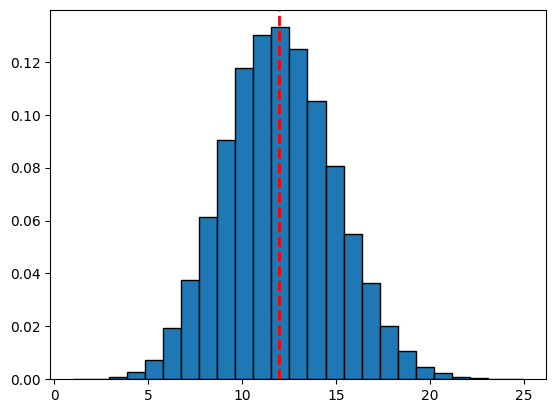
\includegraphics[width=0.7\textwidth]{figures/fig-consecutives-shuffled.png}
\caption{(Normalized) histogram of the number of consecutive pairs of the same suit, over $50,000$ trials. The red dashed line is the empirical mean.}
\end{figure}
Looks like this expected number is something like 12.\marginnote{Try to see what changes if you change the number of cards in the deck (for instance, 34 cards from each suit instead of 13). Could you have predicted it?} How do we explain this?

\begin{theorem}
    The expected number of consecutive same-suit pairs is 12.
\end{theorem}
\begin{proof}
    ``Linearity of expectation.''\marginnote{$\forall i$, $\probaOf{X_i = X_{i+1}} = \frac{13-1}{52-1}$}
\end{proof}

\subsection{One for the rainy days.} It's raining, and all $n$ students of the class come to the lecture with an umbrella. They all leave it in front of the lecture hall. At the end of the lecture, they leave the room in (uniformly) random order, and crossing the door each takes the closest remaining umbrella. In expectation, \emph{how many leave with their own umbrella}?

\begin{theorem}
    The expected number of fixed points in a uniformly random permutation of $\{1,2\dots,n\}$ is one.
\end{theorem}

%%%%%%%%%%%%%%%%%%%%%%%%%%%%%%%%%%%%%%%%%%%%%%%%%%%%%%%%%%%%%%%%%%%%%%%%%%
\section{What's a randomized algorithm?}
Randomized algorithms are algorithms whose behaviour \emph{does not
depend solely on the input.} It also depends (in part) on random
choices or the values of a number of \emph{random bits}.\smallskip

So we can think of the algorithm $\Algo$ as taking an input $x$ and a string of uniformly random bits $R\in\bool^\ast$. Now, since $\Algo$ is randomised, this could mean several things:
\begin{enumerate}
    \item The time $\tau_{\Algo}(x; R)$ that $\Algo$ takes on input $x$ is itself random, and depends on the random bits $R$
    \item The output $\Algo(x;R)$ of $\Algo$ on input $x$ is random, and can be different based on the random bits $R$
    \item Something else (\eg the amount of memory used by $\Algo$ could depend on the random bits)
    \item all, or any combination of the above
\end{enumerate}

Typically, what we want is then analyze $\Algo$ on \emph{worst-case} input $x$ and \emph{uniformly random} $R$. The two things to keep in mind: (1)~is the output of $\Algo$ always correct? Is it correct with high probability (over the choice of random bits $R$)? (2)~is the running time of $\Algo$ always bounded? Is it bounded with high probability, or in expectation (over the choice of random bits $R$)?\marginnote{\advancedstuff{} For those interested, for decision problems this is related to complexity classes \textsf{ZPP}, \textsf{RP}, and \textsf{BPP}. Think of that last one as ``randomized \textsf{P}.''}

\begin{description}
    \item[Las Vegas algorithms:] the algorithm is \emph{always correct}, but the running time is only bounded \emph{in expectation}. 
    \item[Monte-Carlo algorithms:] the algorithm is only \emph{correct with high probability}, but the running time is bounded \emph{with probability one}. 
\end{description}

This is very abstract right now, so before moving to the subtantial example of QuickSort (soon), here is an example:
\begin{framed}
    Given an (arbitrary) array of size $\ns$ containing all numbers from $1$ to $\ns$, output the index of an even number.
\end{framed}
\begin{claim}[Bad news]
Any deterministic algorithm  for this task must have worst-case time complexity $\Omega(\ns)$.
\end{claim}
\begin{claim}[Good news]
There is a Las Vegas algorithm for this task with \emph{expected} time complexity $O(1)$.
\end{claim}
% Pick one until you find one. Expected timesum_k k/2^k = O(1)
\begin{claim}[Good news]
There is a Monte Carlo algorithm for this task with \emph{worst-case} time complexity $O(1)$, and probability of success $0.99$.
\end{claim}
% Pick one k=log2(100) times: failure <= 1/100

\subsection{Relation to other notions of analysis.} What you have focused so far in algorithms classes is \emph{worst-case analysis}: this quantifies the worst possible behaviour of an algorithm (its time complexity, or space complexity, usually), that is, how badly it will do \emph{on the worst possible input you can give it}. This is very useful to know, since once you have figured that out then you know that, no matter what, your
algorithm cannot do worse than that, even on the most adversarial situation. But there are other types of analysis, less frequent and usually much harder to interpret, that can be used: \emph{expected
time analysis} (when the algorithm is randomized: \textbf{this class}), \emph{average time analysis} (when
the input itself comes from some known probability distribution: \textbf{not now}), \emph{amortized
analysis} (when we use the algorithm repeatedly on a sequence of inputs, and look at the worst-case sequence of input for the algorithm divided by the length of the sequence).

\paragraph{Summary:} if $\tau_{\Algo}(x)$ is the time taken by $\Algo$ on input $x$ of size
$|x|$ and $\Algo_k(x_1,\dots,x_k)$ corresponds to running the algorithm successively on
inputs $x_1, \dots, x_k$, then the time analyses discussed above correspond to:
\begin{align*}
    T(\ns) &= \max_{x: |x|=\ns} \tau_{\Algo}(x) \tag{Worst-case} \\
    T_{\rm{}expected}(\ns) &= \max_{x: |x|=\ns} \bE{R}{\tau_{\Algo}(x;R)} \tag{Expected: $\Algo$ is randomized} \\
    T_{\rm{}average}(\ns) &= \bE{x}{\tau_{\Algo}(x)} \tag{Average-case: $x$ is random} \\
    T_{\rm{}amortized}(\ns) &= \lim_{k\to\infty} \frac{1}{k}\max_{|x_1|=\dots=|x_k|=\ns} \tau_{\Algo_k}(x_1,\dots,x_k) \tag{Amortized}
\end{align*}
Again, you probably focused on the first in previous studies, and in this unit we will also consider the second.

\subsection{But why?}
\noindent Some of the reasons for using randomization:
\begin{itemize}
    \item Quickly finding representative or relevant parts of the input (\eg sampling data from a large dataset)
    \item Avoid pathological corner cases
    \item Avoid predictable outcomes % Cryptography, privacy
    \item Allow for simpler or more efficient algorithms
    \item \dots\marginnote{Can you think of anything else?}
\end{itemize}
Some drawbacks:
\begin{itemize}
    \item The behaviour of the algorithm is, well, random. The output might be, or the running time, or something else. Are you happy with this non-deterministic behaviour?
    \item Where do you find these ``random bits'' the algorithm needs?\marginnote{Any idea?}
\end{itemize}
%%%%%%%%%%%%%%%%%%%%%%%%%%%%%%%%%%%%%%%%%%%%%%%%%%%%%%%%%%%%%%%%%%%%%%%%%%
\section{Analyzing Randomized Quicksort}\marginnote{Is this a Las Vegas or a Monte Carlo algorithm?}

Remember QuickSort from your previous classes? It's a very nice comparison-based sorting algorithm, which works as follows:
\begin{algorithm}
\begin{algorithmic}[1]
    \Require Input array $A$ of size $\ns$
    \If{$\ns\leq 1$} \Return $A$
    \EndIf
    \State\label{algo:line:pivot} Select an index $1\leq i\leq \ns$, and let $p \gets A[i]$ be the \emph{pivot}
    \State Partition $A$ into 3 subarrays: $A_1$ (elements smaller than $p$), $A_2$ (equal to $p$), and $A_3$ (greater than $p$) \Comment{ $O(\ns)$ time}
    \State Recursively call QuickSort on $A_1$ and $A_3$ to sort them
    \State Merge the (sorted) $A_1$, $A_2$, $A_3$ into $A$ \Comment{ $O(\ns)$ time}
    \State \Return $A$
\end{algorithmic}
\caption{\textsc{QuickSort}}
\end{algorithm}
This is the prototypical example of a divide-and-conquer algorithm: the only thing unspecified above is \emph{how to choose the pivot}. And this is very important: the time complexity of the whole algorithm depends crucially on it!

The naive way to choose the pivot deterministically (just pick, say, $i=\clg{\ns/2}$) is quite terrible, leading to a worst-case time complexity of $O(\ns^2)$. Not so ``quick.'' A much more involved way to do so, getting the \emph{median} as pivot using linear-time selection\marginnote{If you don't remember what it is, that's alright~--~but it's worth looking it up.} does give sorting in worst-case $O(\ns\log\ns)$ time: but now the algorithm is very complicated, and not so fast in practice anymore.

But this is a class on randomized algorithm, so let's do the obvious randomized thing, and pick the pivot uniformly at random: in~\cref{algo:line:pivot}, choose $i$ uniformly at random in $\{1,2,\dots,\ns\}$. This gives us \emph{Randomized QuickSort}. The proof of correctness is the same as usual QuickSort, but what about the (expected) time complexity? \emph{How fast is it?}

Well, the expected time complexity $T(\ns)$ satisfies the recurrence:
\begin{equation}
    \label{eq:quicksort}
T(\ns) = \bEE{T(|A_1|) + T(|A_2|)} + O(\ns)
\end{equation}
where the expectation is over the random choice of pivot in~\cref{algo:line:pivot}; and $T(1) = O(1)$.

Suppose for simplicity that all elements are distinct.\marginnote{Curious? See how to adapt the proof below to the general case.} Then, if pick pick as pivot the $k$-th largest element, $n_L=k-1$ and $n_R = n-k$. What is the probability to pick the $k$-th largest element as pivot? We select the pivot uniformly at random, so that's $1/n$.

So we can rewrite (the $c\ns$ is for the $O(\ns)$ in~\eqref{eq:quicksort}, which comes from the Divide and the Conquer steps): 
\begin{align*}
 T(\ns) &= c \ns + \frac{1}{n}\sum_{k=1}^{\ns} (T(k-1)+T(\ns-k) ) \\
&= c \ns + \frac{1}{\ns}\sum_{k=0}^{\ns-1} {T(k)}+ \frac{1}{\ns}\sum_{\ell=0}^{n-1} {T(\ell)}
\end{align*}
That is,
\begin{align}
\label{eq:quicksort:rand}
T(\ns) = c \ns + \frac{2}{\ns}\sum_{k=0}^{\ns-1} {T(k)}
\end{align}
Now, \emph{how do we solve this?}\marginnote{Any idea?}

\paragraph{First method: guess, and prove inductively.}
You know the drill. Magically guess $T(\ns) \leq a\ns\log\ns$, try to prove it by induction, see it doesn't quite work depending on which bound you use for $\sum_{k=1}^\ns k\log k$, maybe change your ``magic guess'' to $T(\ns) \leq a\ns\log\ns - b\ns$ to make it work (or get a better bound for the sum).

\paragraph{Second method: integrals are nicer than sums.}
Instead of solving~\cref{eq:quicksort:rand} directly, let's instead compare this discrete relation to a (much nicer to solve) differential equation. The idea is that often, ``sums and integrals are basically the same thing,''
\begin{fact}
    Let $f$ be a non-decreasing function. Then, for all $\ns \geq 0$,
    \[
        \int_0^\ns f(x)dx \leq \sum_{k=0}^\ns f(k) \leq \int_1^{\ns+1} f(x)dx
    \]
\end{fact}
Let's apply that here, and solve the functional equation\marginnote{We make a few implicit (reasonable) assumptions on $T$ here: which ones?}
\[
T(x) = cx + \frac{2}{x}\int_{0}^x T(u) du, \qquad x>0
\]
Introducing the antiderivative $F(x) = \int_{0}^x T(u) du$, we can rewrite this as 
\begin{align}
\label{eq:quicksort:diff:eq}
F'(x) = cx + \frac{2}{x}F(x)
\end{align}
which is ``easier'' to solve,\footnote{Check with an automated solver like Mathematica first: \url{https://www.wolframalpha.com/input?i=solve+F\%27\%28x\%29+\%3D+c+x+\%2B+2\%2Fx+F\%28x\%29+}.} and will lead to $T(x) = O(x \log x)$ and so $T(\ns) = O(\ns\log\ns)$. The point is that differential equations are often much easier to solve than discrete recurrence relations.

\paragraph{\advancedstuff How:} dividing everything by $x^2$, \cref{eq:quicksort:diff:eq} becomes $$ \frac{F'(x)}{x^2} - \frac{2}{x^3} F(x) = \frac{c}{x} $$ but then, we can use that $\frac{d}{dx} \frac{F(x)}{x^2} = \frac{F'(x)}{x^2} - \frac{2F(x)}{x^3}$, so integrating we get $$ \frac{F(x)}{x^2} = c\ln x + C $$ for some constant $C\in\mathbb{R}$, and so $F(x) = c x^2 \ln x + C x^2$. Then $f(x)=F'(x) = 2c x \ln x + (2C+1) x = O(x \log x)$, and we are done.

What we have shown is the following:
\begin{theorem}
    Randomized QuickSort has expected running time $\bigO{\ns\log\ns}$.\marginnote{But still worst-case running time $O(\ns^2)$.}
\end{theorem}

What about the number of \emph{comparisons}? Clearly, what we just showed implies that the expected number of comparisons is also $\bigO{\ns\log\ns}$, but if that's all we are interested in, could we have proven it in a nicer way?
\begin{theorem}
    The expected number of comparisons performed by Randomized QuickSort is $\bigO{\ns\log\ns}$.
\end{theorem}
\begin{proof}
    When we run QuickSort, all the comparisons at one level of the recurrence are between the current pivot and all the other $\ns-1$ elements, and we never compare two elements twice. So we \emph{could} try to solve the corresponding recurrence on the expected number of comparisons $C(\ns)$:
    \begin{equation}
    \label{eq:quicksort:comparisons}
    C(\ns) = \bEE{C(|A_1|) + C(|A_2|)} + (\ns-1)
    \end{equation}
    We could, but we will not.\marginnote{This is the same as for $T(\ns)$, but with an explicit constant instead of $c$.} Instead, here's a slightly nicer argument based on linearity of expectation.

    Suppose for simplicity that all $\ns$ elements are distinct\marginnote{Intuitively, duplicate elements can only make the expected number of comparisons smaller. Can you argue why?} and let us denote them, in ranked order, by
    \[
    a_1 < a_2 < a_3 < \dots < a_\ns
    \]
    (note that this is only for the analysis, and that $a_i$ is not necessarily the element at index $i$ of $A$: the array is generally not already sorted!)
    For any two indices $i < j$, let $X_{ij}\in\{0,1\}$ be the indicator variable of whether Randomized QuickSort ever compares $a_i$ and $a_j$. Since the algorithm never compares twice the same two elements, we have that the total number of comparisons is 
    \[
        X \eqdef \sum_{i=1}^{\ns-1} \sum_{j=i+1}^\ns X_{ij}
    \]
    and $C(\ns) = \bEE{X}$. By linearity of expectation,
    \[
        C(\ns) = \sum_{i=1}^{\ns-1} \sum_{j=i+1}^\ns \bEE{X_{ij}}
        = \sum_{i=1}^{\ns-1} \sum_{j=i+1}^\ns \probaOf{a_i\text{ and } a_j \text{ are compared}}
    \]
    So it boils down to understanding the probability Randomized QuickSort ever compares two fixed distinct elements of the array. Suppose we are at the ${\blue{\ell}}$-th recursive step of the algorithm, with $a_i,a_j$ both in the current subarray of size $\ns_{\blue{\ell}}$, and we pick a pivot $p$:
    \begin{itemize}
        \item If $a_i < p < a_j$, then we will recurse on two disjoint subarrays, one containing $a_i$ and the other $a_j$, so that they will never be compared (decision made!). This happens with probability $\frac{j-i-1}{\ns_{\blue{\ell}}}$.
        \item If $p$ is either $a_i$ or $a_j$, then they will be compared~--~since elements are only compared to the pivot (decision made!). This happens with probability $\frac{2}{\ns_{\blue{\ell}}}$.
        \item Otherwise, they are not compared at this stage, but they both end up in the same subarray the algorithm recurses on, so the comparison could happen later on. This ``no decision either way yet'' happens with probability $1-\frac{j-i+1}{\ns_{\blue{\ell}}}$.
    \end{itemize}
    From the above, we have
    \[
        \probaCond{\substack{a_i\text{ and } a_j\\\text{ are compared}\\\text{at stage }{\blue{\ell}}} }{\substack{\text{Decision made}\\\text{at stage }{\blue{\ell}}}}
        = \frac{\frac{2}{\ns_{\blue{\ell}}}}{\frac{j-i-1}{\ns_{\blue{\ell}}}+\frac{2}{\ns_{\blue{\ell}}}}
        = \frac{2}{j-i+1}
    \]
    Overall, we can write
    \begin{align*}
        \probaOf{\substack{a_i\text{ and } a_j\\\text{ are compared}}}
        &= \sum_{{\blue{\ell}}=0}^\infty \probaCond{\substack{a_i\text{ and } a_j\\\text{ are compared}\\\text{at stage }{\blue{\ell}}} }{\substack{\text{Decision made}\\\text{at stage }{\blue{\ell}}}}
        \probaOf{\substack{\text{Decision made}\\\text{at stage }{\blue{\ell}}}}\\
        &= \sum_{{\blue{\ell}}=0}^\infty \frac{2}{j-i+1}\cdot \probaOf{\substack{\text{Decision made}\\\text{at stage }{\blue{\ell}}}} \\
        &= \frac{2}{j-i+1}\,,
    \end{align*}
    the last line since probabilities sum to one. 
    We are almost there: remember that we are interested in $C(\ns)$, which we now are able to express as
    \[
    C(\ns) = \sum_{i=1}^{\ns-1} \sum_{j=i+1}^\ns \frac{2}{j-i+1}
    = 2\sum_{i=1}^{\ns-1} \sum_{k=1}^{\ns-i} \frac{1}{k+1}
    \]
    This may not look so nice, but letting $H_k = \sum_{i=1}^k \frac{1}{k} \leq \ln k + 1$ denote the $k$-th Harmonic number, we get
    \[
    C(\ns) = 2\sum_{i=1}^{\ns-1}( H_{\ns-i+1} - 1 )
    = 2\sum_{i=2}^{\ns} ( H_i - 1 )
    \leq 2\sum_{i=2}^{\ns} \ln i \leq 2\ns\ln \ns
    \]
    (we even get an explicit upper bound, not just $O(\ns\log\ns)$).
\end{proof}


%%%%%%%%%%%%%%%%%%%%%%%%%%%%%%%%%%%%%%%%%%%%%%%%%%%%%%%%%%%%%%%%%%%%%%%%%%
\section{A few useful probabilistic facts}
Let $X$ be a random variable (r.v.) taking real values: for instance, in $\R$ or $\N$. We assume $X$ has an expectation and a variance.\footnote{This is not necessarily always true! Some random variables do not even have a well-defined expectation. For instance, the random variable defined on $\Z$ by $\probaOf{X=k} = \frac{1}{C}\cdot \frac{1}{1+k^2}$ with $C = 1+\pi\coth \pi$ (so that the probabilities sum to 1) is well-defined, but does not have an expectation since $\sum_{k\in\Z}k\cdot \probaOf{X=k}$ is not defined (does not converge).} A few useful things:
\begin{fact}
If $X$ takes values in $\N = \{0,1,2,\dots,\}$,
\[
\bEE{X} = \sum_{n=0}^\infty n\probaOf{X=n} = \sum_{n=1}^\infty\probaOf{X \geq n}
\]
\end{fact}
To remember whether the sum in the last expression starts at $n=0$ or $n=1$: either reprove it (a bit time-consuming), or take $X$ to be the ``useless'' random variable equal to 0 with probability 1. Then $\bEE{X}=0$, but $\sum_{n=0}^\infty\probaOf{X \geq n} = \probaOf{X \geq 0} = 1$. So we shouldn't have the term $n=0$.

\begin{fact}
If $X$ has a finite variance,
\[
\var[X] = \bEE{(X-\bEE{X})^2} = \bEE{X^2}-\bEE{X}^2
\]
\end{fact}
As a direct consequence, $\var[X]\leq \bEE{X^2}$ (sometimes useful).

\begin{lemma}[Jensen's Inequality]
If $f\colon\R\to\R$ is convex (and $\bEE{f(X)}$ is well-defined)
\[
f(\bEE{X}) \leq \bEE{f(X)}\,.
\]
For $f$ concave, the inequality is reversed.
\end{lemma}
To remember the direction: check with $f(x)=x^2$ (convex). The variance is non-negative, so $0 \leq \var[X] = \bEE{X^2}-\bEE{X}^2$.

\begin{fact}[Linearity of Expectation]
For any $X,Y$ and $a, b \in \R$,
\[
\bEE{aX+bY} = a\bEE{X}+b\bEE{Y}
\]
(We do \emph{not} need $X,Y$ to be independent!)
\end{fact}
\noindent This extends to more random variables: for instance, $\bEE{\sum_{i=1}^n X_i} = \sum_{i=1}^n \bEE{X_i}$. (No independence needed!)

\begin{fact}[Variance]
For any $X$ and $a \in \R$,
\[
\var[aX] = a^2 \var[X]\,.
\]
Moreover, if $X,Y$ are \emph{independent}, 
\[
\var[aX+bY] = a^2 \var[X]+b^2 \var[Y]\,.
\]
\end{fact}
More generally, \textbf{if} $X_1,\dots, X_n$ are mutually independent (or, weaker condition, \emph{pairwise independent}: any two $X_i,X_j$ with $i\neq j$ are independent, but $X_1,\dots, X_n$ as a whole might not be mutually independent.), then
\begin{equation}
\var\mleft[\sum_{i=1}^n X_i\mright] = \sum_{i=1}^n \var[X_i].
\end{equation}
The proof is not too hard: basically, since $\var[X] = \bEE{(X-\bEE{X})^2}$, consider 
$\bEE{\Paren{\sum_{i=1}^n (X_i-\bEE{X_i})}^2}$ and expand the square, then use linearity of expectation:
\begin{align*}
\var\mleft[\sum_{i=1}^n X_i\mright] 
&= \bEE{\sum_{i=1}^n\sum_{j=1}^n (X_i-\bEE{X_i})(X_j-\bEE{X_j})} \\
&= \bEE{\sum_{i=1}^n(X_i-\bEE{X_i})^2} + \bEE{\sum_{i\neq j} (X_i-\bEE{X_i})(X_j-\bEE{X_j})}\\
&=\sum_{i=1}^n\bEE{(X_i-\bEE{X_i})^2} + \sum_{i\neq j} \bEE{(X_i-\bEE{X_i})(X_j-\bEE{X_j})}
\end{align*}
The first term is exactly $\sum_{i=1}^n\var[X_i]$; the second, by pairwise independence, is 0, since $\bEE{(X_i-\bEE{X_i})(X_j-\bEE{X_j})} = \bEE{(X_i-\bEE{X_i})}\bEE{(X_j-\bEE{X_j})} = 0\cdot 0$.\medskip


Now, a few very trivial-looking (but useful!) facts. Suppose $X$ takes values in $\{0,1\}$, with $\probaOf{X=1}=p$ (this is a Bernoulli random variable). Then
\begin{itemize}
    \item $X^2=X$ (of course!), so $\bEE{X^2}=\bEE{X}=\probaOf{X=1}=p$
    \item That implies $\var[X] = \bEE{X^2}-\bEE{X}^2 = p-p^2 = p(1-p)$, which is at most $1/4$.\marginnote{Check it! $x(1-x)\leq 1/4$ for $x\in[0,1]$, and the maximum is at $x=1/2$.}
    \item That implies that for a Binomial $X\sim\binomial{n}{p}$, which is just the sum of $n$ \emph{independent, and identically distributed} (\iid) Bernoullis with parameter $p$,
    \[
        \bEE{X} = np, \qquad \var[X] = np(1-p)\,.
    \]
\end{itemize}
Finally, an \emph{indicator} random variable (for some ``event'' $E$) is just a Bernoulli random variable which is equal to 1 if the event occurs, and 0 otherwise (so, Bernoulli with parameter $\proba(E)$). Usually denoted $\indicSet{E}$.

\chapter{Lecture 2: Concentration Bounds, and Tricks}\label{chap:2}
\section{Markov goes to Las Vegas}

Remember from last lecture that we saw two types of randomised algorithms: {Las Vegas} and {Monte Carlo}.\marginnote{There are more, of course: \eg Bellagio algorithms. And others! Mathematicians and computer scientists clearly love gambling~--~look up Jacob Bernoulli when you have a chance.}

\begin{quote}
\begin{description}
    \item[Las Vegas algorithms:] the algorithm is \emph{always correct}, but the running time is only bounded \emph{in expectation}. 
    \item[Monte-Carlo algorithms:] the algorithm is only \emph{correct with high probability}, but the running time is bounded \emph{with probability one}. 
\end{description}
\end{quote}
Wouldn't it be nice if there was a way to go from one to the other? Well, as it turns out, there is:
\begin{lemma}
    \label{lemma:lvtomc}
    Suppose there exists a Las Vegas algorithm $\Algo$ for some task, with expected running time $\blue{T}$. Then there exists a Monte Carlo algorithm $\Algo'$ for the same task with \emph{worst-case} running time $O(\blue{T})$ and probability of failure $1/100$.
\end{lemma}
\begin{proof}
The proof is quite simple, and relies on analyzing the following:
\begin{algorithm}[H]
\begin{algorithmic}[1]
    \Require input $x$
    \State Run $\Algo$ on $x$ for at most $100\blue{T}$ steps
    \If{$\Algo$ terminated within $100\blue{T}$ steps}
        \State\label{markov:line:goodoutput}\Return $\Algo$'s output \Comment{Always correct}
    \Else 
        \State\label{markov:line:mehoutput}\Return an arbitrary output \Comment{Very likely wrong}
    \EndIf
\end{algorithmic}
    \caption{Algorithm $\Algo'$.}
\end{algorithm}
It should be quite clear that the above algorithm always runs in time at most $100\blue{T} + O(1) = O(\blue{T})$; and also that whenever we reach~\cref{markov:line:goodoutput}, the output of $\Algo'$ must be correct (because $\Algo$, once it terminates, is always correct). 

When we reach~\cref{markov:line:mehoutput} because $\Algo$ ``timed out,'' however, we cannot really say anything: maybe what we output is correct, but it's most likely wrong. So we'll just assume it's an incorrect output, and all we need to do to prove the lemma is to prove that $\Algo$ ``times out'' with probability at most $1/100$.

Importantly, all we can use to do so is what we know about $\Algo$, which is very little: we only know its expected running time is at most $\blue{T}$, and that running times are non-negative. That's not a lot to build on, but that's just enough for \emph{Markov's inequality}:

\begin{theorem}[Markov's inequality]
Let $X$ be a non-negative\marginnote{The ``non-negative'' assumption is crucial. It is definitely not true without!} random variable with $\bEE{X} < \infty$. For any $t > 0$, we have
\[  
  \bPr{ X \geq t } \leq \frac{\bEE{X}}{t}
\]
\end{theorem}
\noindent Applying this with $X$ being the running time of $\Algo$ and $t=100$ proves the lemma.
\end{proof}
\marginnote{Lecture cue: prove Markov's.}
%%%
% Should I mention the algorithmic Jensen paper?
%%%
\section{Markov and beyond: Randomised Median}
% Useful/good: https://www.cs.dartmouth.edu/~deepc/LecNotes/Rand/lec6.pdf
As mentioned in the previous lecture, there exists a very neat, highly non-trivial (deterministic) divide-and-conquer algorithm to find the median of (an array of) $\ns$ numbers in linear time. You have seen it in previous  So we will not analyze it again: instead, we will give a simple (Monte Carlo) randomized algorithm, also linear-time. 

The idea of the algorithm is relatively simple, yet surprisingly powerful: given as input an array $\red{A}$ of $\ns$ integers\marginnote{For simplicity, we will throughout assume $\ns$ is odd, and that all numbers are distinct. Neither of these assumptions is necessary.}, subsample at random a \emph{smaller} array $\orange{B}$ of $\orange{m} \ll \ns$ integers from $\red{A}$, and use $\orange{B}$ as some sort of ``guide'' for what is in $\red{A}$. In particular, we expect, if we are not too unlucky, that finding ``approximate medians'' of $\orange{B}$ will give us an approximate idea of what the median of $\red{A}$ is, and we can then filter out a lot of the elements of $\red{A}$ to end up with a much more manageable task. And we can easily find that in $\orange{B}$, since it will have much smaller size!

Here is the actual algorithm, only missing the value of $\orange{m}$ (to be determined shortly):
\begin{algorithm}[H]
\begin{algorithmic}[1]
    \Require array $\red{A}$ of $\ns$ distinct integers
    \State Set $\Delta = 4\sqrt{\orange{m}}$ \Comment{Why? We'll see later. ``Chebyshev.''}
    \State Create an array $\orange{B}$ containing $\orange{m}$ elements of $\red{A}$ chosen independently and uniformly at random (with replacement)
    \State Sort $\orange{B}$ \Comment{Time $O(\orange{m}\log \orange{m})$}
    \State Let $\underline{b}$ and $\overline{b}$ be the $(\orange{m}/2-\Delta)$-th and $(\orange{m}/2+\Delta)$-th elements of $\orange{B}$ \Comment{``Approximate medians'' of $\orange{B}$}
    \State \Comment{Now we use $\underline{b}$ and $\overline{b}$ as ``guides'' for the contents of $\red{A}$. All 3 steps below take time $O(\ns)$.}
    \State\label{step:lintime:1} Copy every $x$ of $\red{A}$ with $\underline{b}\leq x\leq \overline{b}$ in a new array $\blue{C}$
    \State\label{step:lintime:2} Compute the number $k$ of elements of $\red{A}$ smaller than $\underline{b}$ 
    \State\label{step:lintime:3} Compute the number $\ell$ of elements of $\red{A}$ larger than $\overline{b}$ 
    \If{$k > \frac{\ns}{2}$ or $\ell > \frac{\ns}{2}$}
        \State\Return \textsf{fail} \Comment{The median of $\red{A}$ cannot be in $\blue{C}$}
    \ElsIf{$|\blue{C}| > \frac{4\ns\Delta}{\orange{m}}+2$}
        \State\Return \textsf{fail} \Comment{We cannot process $\blue{C}$ fast enough!}
    \Else
        \State Sort $\blue{C}$  \Comment{Time $O\big(\frac{\ns}{\sqrt{\orange{m}}}\log \frac{\ns}{\sqrt{\orange{m}}}\big)$}
        \State\label{step:return:median}\Return the $(\frac{\ns+1}{2}-k)$-th element of $\blue{C}$.
    \EndIf
\end{algorithmic}
    \caption{Randomised Median in Worst-Case Linear Time.}
    \label{algo:randomized:median}
\end{algorithm}

First, let's look at the time complexity. Assuming for now that $\orange{m} = \bigO{\ns/\log\ns}$ and $\frac{4\ns\Delta}{\orange{m}} = \bigO{\ns/\log\ns}$ (they will be!), the total time is dominated by~\cref{step:lintime:1,step:lintime:2,step:lintime:3}, and so the algorithm runs in (worst-case) time $O(\ns)$. Good.

Second, let's look at the correctness. Suppose the algorithm reaches~\cref{step:return:median}: then it not hard to see that the element returned is at position $k+\frac{\ns+1}{2}-k = \frac{\ns+1}{2}$ in $\red{A}$: that is, it indeed returns the median. 

So the algorithm always runs in time $O(\ns)$, and when it does not output \textsf{fail} it correctly outputs the median of $\red{A}$. This only leaves us with the third point: \emph{what is the probability the algorithm returns \textsf{fail}?}

This can only happen because of three things (``bad events''):
\begin{description}
    \item[Event ${E}_1$:] Too many elements are smaller than $\underline{b}$: $k > \frac{\ns}{2}$
    \item[Event ${E}_2$:]  Too many elements are larger than $\overline{b}$: $\ell > \frac{\ns}{2}$
    \item[Event ${E}_3$:]  $\blue{C}$ is too large: $|\blue{C}| > \frac{4\ns\Delta}{\orange{m}}+2$\marginnote{Why is that an issue, again?}
\end{description}
We want to get an upper bound on the probability \emph{at least one} of these three events occurs. We could try to argue these events are independent (maybe?) and try to bound $\probaOf{E_1\cup E_2\cup E_3} = 1-\probaOf{\overline{E_1}\cap\overline{E_2}\cap\overline{E_3}}$, and maybe (?) get some reasonable bound as a result. But independence is tricky to reason about, and nobody wants to do that if they do not have to. So instead, we will use the \emph{union bound}:\marginnote{The union bound sounds basic, but it is truly a fundamental, powerful tool.}
\begin{lemma}[Union Bound]
Let $E_1,\dots,E_k,\dots$ be a (possibly countably infinite) family of (possibly dependent) events. Then
\[
    \probaOf{ \bigcup_{k=1}^\infty E_k } \leq \sum_{k=1}^\infty \probaOf{E_k}\,. 
\]
\end{lemma}
This is great! No need to worry about independence: now we immediately have by the union bound that
\begin{equation}
    \label{eq:first:union:bound}
    \probaOf{E_1\cup E_2\cup E_3} \leq \probaOf{E_1}+\probaOf{E_2}+\probaOf{E_3}\,.
\end{equation}
By symmetry, one can also convince themselves that $\probaOf{E_1}=\probaOf{E_2}$, so we only have two things to analyze.

\paragraph{Bounding $\probaOf{E_1}$.} What is the probability that $k$, the number of elements of $\red{A}$ smaller than $\underline{b}$, exceeds $\frac{\ns}{2}$? By definition, if it exceeds $\frac{\ns}{2}$, then $\underline{b}$ is larger than (or equal to) the median of $\red{A}$. But $\underline{b}$ is the $(\frac{\orange{m}}{2} - \Delta)$-th element of $\orange{B}$, which means that among the $\orange{m}$ elements we picked uniformly at random (with replacement) to create $\orange{B}$, at most $\frac{\orange{m}}{2} - \Delta$ were smaller than the median.

Which should be unlikely: when we pick \emph{one} element uniformly at random from $\red{A}$, the probability to get an element smaller than the median is exactly $\frac{\ns-1}{2}\cdot \frac{1}{\ns} = \frac{1}{2} - \frac{1}{2\ns}$. So ``by linearity of expectation'' the expected number of elements smaller than the median is $\frac{\orange{m}}{2} - \frac{\orange{m}}{2\ns}$. But $\frac{\orange{m}}{2} - \Delta$, that's \emph{much} smaller than that! Can we quantify this?

Thankfully yes. Let's call ``the expected number of elements smaller than the median'' $X$. Then we can write $X = \sum_{i=1}^{\orange{m}} X_i$, where $X_i\in\{0,1\}$ is the indicator random variable for ``the $i$-th element sampled to go into $\orange{B}$ was smaller than the median of $\red{A}$.'' That is, all $X_i$s are \iid, and Bernoulli random variables with parameter $p \eqdef \frac{1}{2} - \frac{1}{2\ns}$,\marginnote{This means $X$ is a {Binomial} random variables with parameters $\orange{m}$ and $p$: $X\sim \binomial{\orange{m}}{p}$.} and so from what we saw about Binomials last week we get that $\var[X] = \orange{m}p(1-p) = \frac{\orange{m}}{4}\left(1-\frac{1}{\ns^2}\right) < \frac{\orange{m}}{4}$.

Why are we interested in the variance? Good question! We want to argue that most of the time $X$ is ``not too far from its expectation'' $\frac{\orange{m}}{2}\left(1-\frac{1}{\ns}\right)$, and in particular that getting as low as $\frac{\orange{m}}{2} - \Delta = \frac{\orange{m}}{2}\big(1 - \frac{2}{\sqrt{\orange{m}}}\big)$ is truly a freak event.\marginnote{Do it: try and apply Markov's inequality to $X$. Why doesn't it work? Then try to apply it to $\orange{m}-X$: why is the result too weak?} Unfortunately, using Markov's inequality here will not be enough\dots{} we need something stronger. 

And that's where \emph{Chebyshev's inequality} comes into play: instead of just using the expectation, Chebyshev allows you to leverage additional information you may have about the random variable, specifically its variance, to (usually) get stronger bounds:
\begin{theorem}[Chebyshev's inequality]
Let $X$ be a random variable with $\bEE{X^2} < \infty$. For any $t > 0$, we have
\[  
  \bPr{ \abs{X-\bEE{X}} \geq t } \leq \frac{\var[X]}{t^2}
\]
\end{theorem}
Another way to look at it: this is saying that a random variable usually may fluctuate around its expectation by give or take a few standard deviations (\ie a few $\sqrt{\var}$)\dots{} but \emph{more}? That's unlikely. \marginnote{By the way, this is why we set $\Delta = 4\sqrt{\orange{m}}$: the standard deviation of $X$ we computed about is $\approx \sqrt{\orange{m}}/2$, so that's the right order of magnitude.}


\begin{framed}
\noindent Compared to Markov's inequality, Chebyshev's:
\begin{itemize}
    \item Provides \emph{two-sided} bounds (bounds the probability to deviate too far below \emph{and} too far above the expectation) \hfill $\checkmark$
    \item Gives a bound that decays quadratically ($\propto 1/t^2$) instead of linearly ($\propto 1/t$), so is better for $t\geq 1$ (\cref{fig:markov:chebyshev}) \hfill $\checkmark$
    \item Does not require the random variable to be non-negative \hfill $\checkmark$
    \item Requires knowing a bound on the variance (if it exists) \hfill$\times$
\end{itemize}
\end{framed}
\begin{figure}[h]
    \centering
    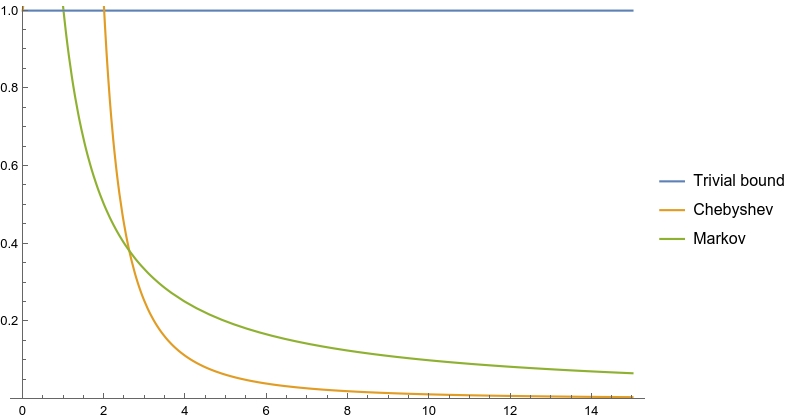
\includegraphics[width=0.9\textwidth]{figures/fig-markov-v-chebyshev.png}
    \caption{An illustration of the tail bounds $\probaOf{X\geq t}$ (as a function of $t\geq 0$) given by Markov and Chebyshev's inequalities, for the specific case of a non-negative random variable $X\geq 0$ with both expectation and variance equal to $1$: $\expect{X}=\var[X]=1$. Note that Chebyshev does not require that $X\geq 0$, this is simply here for the sake of comparison with Markov's inequality, which does.}
    \label{fig:markov:chebyshev}
\end{figure}
So we want to use Chebyshev's inequality to argue $\probaOf{X \leq \frac{\orange{m}}{2} - \Delta}$ is small. Here we go: rewriting $\frac{\orange{m}}{2} - \Delta = \expect{X} - \left(\Delta - \frac{\orange{m}}{2\ns}\right)$ and using $\orange{m}\leq \ns$ (so $\Delta - \frac{\orange{m}}{2\ns} \geq \Delta - \frac{1}{2} \geq \frac{\Delta}{2} = 2\sqrt{\orange{m}}$), we have
\begin{align*}
    \probaOf{X \leq \frac{\orange{m}}{2} - \Delta}
    &= \probaOf{X \leq \expect{X} - \left(\Delta - \frac{\orange{m}}{2\ns}\right)}\\
    &\leq \probaOf{\abs{X-\expect{X}} \geq \left(\Delta - \frac{\orange{m}}{2\ns}\right)}\\
    &\leq \frac{\var[X]}{\big(\Delta - \frac{\orange{m}}{2\ns}\big)^2} \tag{by Chebyshev}\\
    &\leq \frac{\orange{m}}{4(\Delta/2)^2} \tag{Bound on variance}\\
    &= \frac{1}{16} \tag{Setting of $\Delta$} 
\end{align*}
This gives us
\begin{equation}
    \label{eq:bounding:approxmedians:1}
    \probaOf{E_1},\probaOf{E_2} \leq \frac{1}{16}\,,
\end{equation}
using Chebyshev's inequality. We only have to bound $\probaOf{E_3}$ to conclude.

\paragraph{Bounding $\probaOf{E_3}$.} This is the last piece:\footnote{For now at last: there will be more down the line.} we want to bound the probability that $\blue{C}$ is ``too large,'' that is the probability $|\blue{C}|$ exceeds $4\orange{m}$. Since all we have seen so far relies either on computing the expectation of the quantity of interest, its variance, or both, it would seem reasonable to start with computing $\expect{|\blue{C}|}$ and maybe use Markov's inequality: unfortunately,
the quantity $\expect{|\blue{C}|}$ is quite tricky to compute. 

Instead, we will take an alternative path: let $R_{\underline{b}}$ denote the rank of $\underline{b}$ in $\red{A}$ (and similarly $R_{\overline{b}}$ for $\overline{b}$). We have already proven that 
\[
\probaOf{ R_{\underline{b}} > \frac{\ns}{2}} , \probaOf{ R_{\overline{b}} < \frac{\ns}{2}} \leq \frac{1}{16}
\]
(this is~\cref{eq:bounding:approxmedians:1}). Now, we want to prove that $|\blue{C}| = R_{\overline{b}}-R_{\underline{b}} +2 \leq \frac{4\ns\Delta}{\orange{m}}+2$ with high probability: so it'd \emph{suffice} to show that 
\[
\probaOf{ R_{\underline{b}} < \frac{\ns}{2} - 2\frac{\ns\Delta}{\orange{m}}} , \probaOf{ R_{\overline{b}} > \frac{\ns}{2} + 2\frac{\ns\Delta}{\orange{m}}} \leq \frac{1}{32}
\]
as this would imply the result. One may ask: \emph{why these particular values?} The reason is that since $\underline{b}$ is defined as the ($\frac{\orange{m}}{2} - \Delta$)-th element in $\orange{B}$, if the uniform random sampling was ``representative'' enough we expect to have an $\frac{1}{2} - \frac{\Delta}{\orange{m}}$ fraction of the original array $\red{A}$ on its left: so having much less than that, say a fraction $\frac{1}{2} - 2\frac{\Delta}{\orange{m}}$, ``should'' be unlikely.

As before, we will only focus on bounding $\probaOf{ R_{\underline{b}} < \frac{\ns}{2} - 2\frac{\ns\Delta}{\orange{m}}}$, as the case of $R_{\overline{b}}$ is similar (by symmetry). 

To proceed, let's consider the set $S$ of the $s\eqdef \frac{\ns}{2} - 2\frac{\ns\Delta}{\orange{m}}$ smallest elements of $\red{A}$~--~let's call them ``tail elements''. The key observation is that if \emph{fewer} than $\frac{\orange{m}}{2}-\Delta$ elements of $S$ end up in $\orange{B}$, then $\underline{b}$, being the ($\frac{\orange{m}}{2}-\Delta$)-th element of $\orange{B}$, is not a tail element: and so must have $R_{\underline{b}} \geq s$. Based on that, we want to show that the probability to have \emph{at least} $\frac{\orange{m}}{2}-\Delta$ of $S$ in $\orange{B}$ is small.

Now this looks familiar: the probability to pick an element of $S$ when choosing one from $\red{A}$ uniform at random is $\frac{s}{\ns} = \frac{1}{2} - \frac{2\Delta}{\orange{m}}$. The number of elements from $S$ in $\orange{B}$ (call it $Y$) is then a Binomial random variable with parameters $\orange{m}$ and $\frac{s}{\ns}$. We have $\expect{Y} = \frac{\orange{m}s}{\ns} = \frac{\orange{m}}{2}-2\Delta$, $\var[Y] = \frac{\orange{m}s}{\ns}\Paren{1-\frac{s}{\ns}} \leq \frac{\orange{m}s}{\ns} \leq \frac{\orange{m}}{2}$; and we want to bound
\begin{align*}
    \probaOf{Y \geq \frac{\orange{m}}{2}-\Delta}
    &= \probaOf{Y \geq \expect{Y}+\Delta} \\
    &\leq  \probaOf{|Y - \expect{Y}| \geq \Delta} \\
    &\leq \frac{\var[Y]}{\Delta^2} \tag{Chebyshev}\\
    &= \frac{\orange{m}}{2\cdot 16\orange{m}} \tag{as $\Delta= 4\sqrt{\orange{m}}$}\\
    &= \frac{1}{32}
\end{align*}
To summarize, we've just shown that
\[
    \probaOf{ R_{\underline{b}} < \frac{\ns}{2} - 2\frac{\ns\Delta}{\orange{m}}} \leq \probaOf{Y \geq \frac{\orange{m}}{2}-\Delta} \leq \frac{1}{32}
\]
We can similarly get $\probaOf{ R_{\overline{b}} > \frac{\ns}{2} + 2\frac{\ns\Delta}{\orange{m}}} \leq \frac{1}{32}$\marginnote{Do it! That's good practice.}, and so, ``by a union bound,''
\begin{align}
    \probaOf{E_3} &= \probaOf{|\blue{C}| > \frac{4\ns\Delta}{\orange{m}} + 2} \notag\\
    &\leq \probaOf{ R_{\underline{b}} < \frac{\ns}{2} - 2\frac{\ns\Delta}{\orange{m}}} + \probaOf{ R_{\overline{b}} > \frac{\ns}{2} + 2\frac{\ns\Delta}{\orange{m}}} \notag\\
    &\leq \frac{1}{16}\,.
\end{align}

\paragraph{Putting it together.}
The probability that the algorithm fails is bounded, from~\cref{eq:first:union:bound}, by
\[
\probaOf{E_1\cup E_2\cup E_3} \leq \probaOf{E_1}+\probaOf{E_2}+\probaOf{E_3} \leq \frac{1}{16} + \frac{1}{16} + \frac{1}{16} = \frac{3}{16}\,.
\]
When it doesn't fail, we have seen that it is correct; and it \emph{always} runs in time at most $O(\ns)$. So\dots{} we're done! \emph{Almost.} We haven't chosen the value of $\orange{m}$ yet!

So what do we need? For our running time, we need both $O(\orange{m}\log\orange{m})$ and $O(\frac{\ns\Delta}{\orange{m}}\log\frac{\ns\Delta}{\orange{m}}) =O(\frac{\ns}{\sqrt{\orange{m}}}\log \frac{\ns}{\sqrt{\orange{m}}})$ to be $O(\ns)$. There are many ways to do so, but one aesthetically pleasing choice is to make both equal:
\[
    \orange{m} = \frac{\ns}{\sqrt{\orange{m}}}
\]
which leads to setting $\boxed{\orange{m} = \ns^{2/3}}$. To conclude:
\begin{theorem}
    \label{theo:randomized:median}
    Randomised Median (\cref{algo:randomized:median}) is a linear-time Monte Carlo algorithm with failure probability at most $3/16$.
\end{theorem}

\section{But can we bring down this failure probability?}
This is all very good, but, when you think about it, a failure probability of $3/16\approx 19\%$ might be too much for many applications. Can we somehow bring this down to $1\%$? $0.01\%$? $\errprob$, for any $\errprob\in(0,1]$ of our choosing?

The obvious natural approach would be to go back to our analysis, see what the bottlenecks were, and modify the parameters to achieve smaller error probability. This would work \emph{here}\marginnote{\advancedstuff{} Go through the argument and see what happens to the probability of failure when you choose a larger $\Delta$, for instance $\orange{m}^{3/4}$ or $\sqrt{\ns}$.}, but it may not \emph{always} work, and honestly it is also very inconvenient. We went through a lot of trouble to establish~\cref{theo:randomized:median}, it would be nice not to have to start all over again!

Fortunately, it \emph{is} possible: there is a way to take our algorithm (and the guarantees we proved for it), and amplify its success probability \emph{in a blackbox way}. Of course, there is a cost: we will need to run the algorithm several times~--~the price is more computation time, and more random bits.\marginnote{Random bits are not always cheap: they are a resource, like time, and memory.}

Here is the idea: given the input array $\red{A}$ run the algorithm (\cref{algo:randomized:median}) $T$ times on $\red{A}$, using fresh (independent) random bits each time. If at any point the algorithm does not return $\textsf{fail}$, then return the median it outputs. If this never happens, return $\textsf{fail}$.

Since we have a Monte Carlo algorithm, whenever we return something else than $\textsf{fail}$ this is guaranteed to be correct, and we have the median. So what is the probability to output $\textsf{fail}$ now? Well, we need \emph{all} $T$ independent runs to fail. And they are all independent, so the probability that they all fail is at most
\[
    \Paren{\frac{3}{16}}^T
\]
Solving for this to be less than $\errprob$, we get that  taking
\[
    T = \clg{\frac{\log(1/\errprob)}{\log\frac{16}{3}}} = O(\log(1/\errprob))
\]
suffices. This gives the following:
\begin{corollary}
    \label{coro:randomized:median}
    For any $\errprob \in(0,1]$, the Repeated Randomised Median described above is a Monte Carlo algorithm with failure probability at most $\errprob$ and worst-case time complexity $O(\ns\log(1/\errprob))$.
\end{corollary}
\noindent This simple ``trick'' is your first example of \emph{probability amplification.}

\section{Viva Las Vegas!}
In light of~\cref{coro:randomized:median}, it is natural to wonder: why stopping there? Can we convert any Monte Carlo algorithm into a Las Vegas algorithm, providing a converse to~\cref{lemma:lvtomc}?

The answer is \emph{not always} (not for every Monte Carlo algorithm), but in this particular case yes. The key observation is that~\cref{algo:randomized:median} is not \emph{any} Monte Carlo algorithm: it never ``fail silently.'' That is, when the \cref{algo:randomized:median} fails, it tells us so! This is a very valuable feature.

Consider the following algorithm:
\begin{algorithm}[H]
\begin{algorithmic}[1]
    \Require array $\red{A}$ of $\ns$ distinct integers
    \Repeat
        \State Run~\cref{algo:randomized:median} on $\red{A}$ (with fresh random bits)
        \State Let $y$ be the output
    \Until{$y\neq \textsf{fail}$}\label{step:until:exit}
    \State\Return $y$
\end{algorithmic}
    \caption{Randomised Median in Expected Linear Time.}
    \label{algo:randomized:median:lv}
\end{algorithm}
Correctness is immediate: whenever this new algorithm stops, the $y$ it outputs is the median of $\red{A}$. But \emph{does it ever stop}? And if so, what is its expected running time?\medskip

Let $\tau(\ns) = O(\ns)$ be the (worst-case) running time of \cref{algo:randomized:median}, and $K$ be the (random) number of loop iterations before~\cref{algo:randomized:median:lv} terminates. Clearly, the (random) running time of~\cref{algo:randomized:median:lv} is (at most) $K\cdot \tau(\ns)$. What can we say about $K$?\marginnote{Some vocabulary: $K$ as defined here is a \emph{geometric random variable} with parameter $p \geq 13/16$.}
\begin{enumerate}
    \item The probability that $K\geq 1$ is $1$: we always run the loop at least once.
    \item The probability that $K\geq 2$ is at most $3/16$: to go to the second iteration of the loop, the first call to~\cref{algo:randomized:median} must have failed.
    \item The probability that $K\geq 3$ is at most $(3/16)^2$: to go to the third iteration of the loop, the first two calls to~\cref{algo:randomized:median} must have failed (and they are independent).
    \item The probability that $K\geq k$ is at most $(3/16)^{k-1}$: to go to the $k$-th iteration of the loop, the first $k-1$ calls to~\cref{algo:randomized:median} must have failed (and they are independent).
\end{enumerate}
This is particularly useful, since from what we say in the first chapter we can write
\[
    \expect{K} = \sum_{k=1}^\infty \probaOf{K\geq k} 
\]
and here this becomes
\[
    \expect{K} \leq \sum_{k=1}^\infty \Paren{\frac{3}{16}}^{k-1} = \frac{16}{13} \leq  1.231
\]
This means that the expected running time of our Las Vegas algorithm,~\cref{algo:randomized:median:lv}, is at most $1.231\cdot \tau(\ns) = O(\ns)$!
\begin{corollary}
    \label{coro:randomized:median:lv}
    For any $\errprob \in(0,1]$, the Indefinitely Repeated Randomised Median (\cref{algo:randomized:median:lv}) is a Las Vegas algorithm with expected time complexity $O(\ns)$.
\end{corollary}
\noindent More generally, we can prove the following:
\begin{theorem}
    Let $\Algo$ be a Monte Carlo algorithm with worst-case running time $T(\ns)$ and constant failure probability $p\in(0,1)$, with the following extra guarantee: one can detect whether the output of $\Algo$ is incorrect in time $O(1)$. Then there exists a \emph{Las Vegas} algorithm $\Algo'$ for the same task with expected running time $O(T(\ns))$ (where the hidden constant in the $O(\cdot)$ depends on $p$).
\end{theorem}
\begin{proof}
    Your turn!
\end{proof}

\section{And to conclude, something totally different!}\marginnote{Probability amplification by Majority Vote}
The Randomised Median algorithm we saw (\cref{algo:randomized:median}) was quite nice, as far as Monte Carlo algorithms go: whenever it failed, \emph{it told us so.}
But that's usually not the case. Consider for instance the following scenario: someone implemented a very useful thing, say a data structure with its API, and gives you access. You cannot see the code or the implementation to check it's correct: all you can do is query that data structure $\red{D}$, and on input element $\blue{x}$ this query $\green{\mathcal{Q}}$ to $\red{D}$ is supposed to output
\[
    \green{\mathcal{Q}}(\blue{x}) = \begin{cases}
        \yes &\text{if } \blue{x}\in\red{D} \\
        \no &\text{if } \blue{x}\notin\red{D} \\
    \end{cases}
\]
Unfortunately, the implementation is \emph{not} correct, or something is wrong: for whatever reason, each query behaves somewhat randomly, and is only correct with probability $60\%$.\marginnote{This sounds ridiculous? Wait until you hear about hashing and Bloom filters later in the course.} And when it's wrong, of course, you don't know it!

\begin{framed}
    Can we use this data structure access in a blackbox way to obtain better guarantees, and have queries that are correct with probability $99\%$ instead? Probability $1-\errprob$?
\end{framed}

The answer is, again, \emph{yes}. And the probability amplification technique to use here is very intuitive: a simple \emph{majority vote}. Here's what we will do, where $T=T(\errprob)$ is an integer to be determined shortly:
\begin{algorithm}[H]
\begin{algorithmic}[1]
    \Require blackbox access to $\red{D}$ via $\green{\mathcal{Q}}$; input $\blue{x}$
    \For{$t=1,2,\dots, T$}
        \State $y_t \gets \green{\mathcal{Q}}(\blue{x}) \in\{\yes,\no\}$
    \EndFor
    \State\Return $\operatorname{majority}(y_1,\dots,y_T)$ \Comment{$\yes$ if at least half of the $y_t$'s are $\yes$}
\end{algorithmic}
    \caption{More reliable data structure via majority vote.}
    \label{algo:majority:vote}
\end{algorithm}
Let us analyze this. For any fixed $\blue{x}$, we know that each $y_t\in\{0,1\}$ is the correct answer with probability at least $6/10$, and are independent (we assume that the random errors are independent, at least). So if we define
\[
    Y = \sum_{t=1}^T \indic{y_t\text{ is correct}}
\]
we have a sum of independent Bernoulli random variables.\marginnote{It's even a Binomial r.v. with parameters $T$ and $p\geq 6/10$, but we will not need to be that precise.} And since we take a majority vote, the only way for our output to be incorrect is to have \emph{more than half} of the $T$ answers being incorrect, that is, to have $Y < \frac{1}{2}T$.

But $\expect{Y} \geq \frac{6}{10}T$, so to be wrong we need $Y$ to be more than $\frac{1}{10}T$ away from its expectation. This should ring a bell: \emph{we can use Chebyshev's inequality for that!}\smallskip

We \emph{could}, but that will not be good enough (that won't give a good enough bound).\marginnote{Try it: Chebyshev should get you something like $\probaOf{Y < \frac{1}{2}T} \leq \frac{24}{T}$.} We can do better! 
Enters the \emph{Chernoff bound}:
\begin{theorem}[Chernoff bound]
Let $X_1,\dots,X_n$ be \emph{independent} random variables taking value in $[0,1]$, and let $P \eqdef \sum_{i=1}^n \bEE{X_i}$ For any $\gamma \in (0,1]$ we have
\begin{align}
\bPr{\sum_{i=1}^n X_i > (1+\gamma)P } &< \exp(-\gamma^2 P/3)\\
\bPr{\sum_{i=1}^n X_i < (1-\gamma)P } &< \exp(-\gamma^2 P/2)
\end{align}
\end{theorem}
We can apply it with ``$n=T$, $P=\frac{6}{10}T$, and $\gamma=\frac{1}{6}$'' (the last one to have $(1-\gamma)\cdot \frac{6}{10}T = \frac{1}{2}T$), and that immediately gives us
\[
    \bPr{ Y < \frac{1}{2}T } \leq e^{-\frac{1}{120}T}
\]
which decays \emph{exponentially} with $T$.\marginnote{Sure, the constant $1/120$ in there is not great, but we could do better by sweating a bit more.} In particular, for large $T$ this is much, much better than what Chebyshev would give:
\begin{figure}
    \centering
    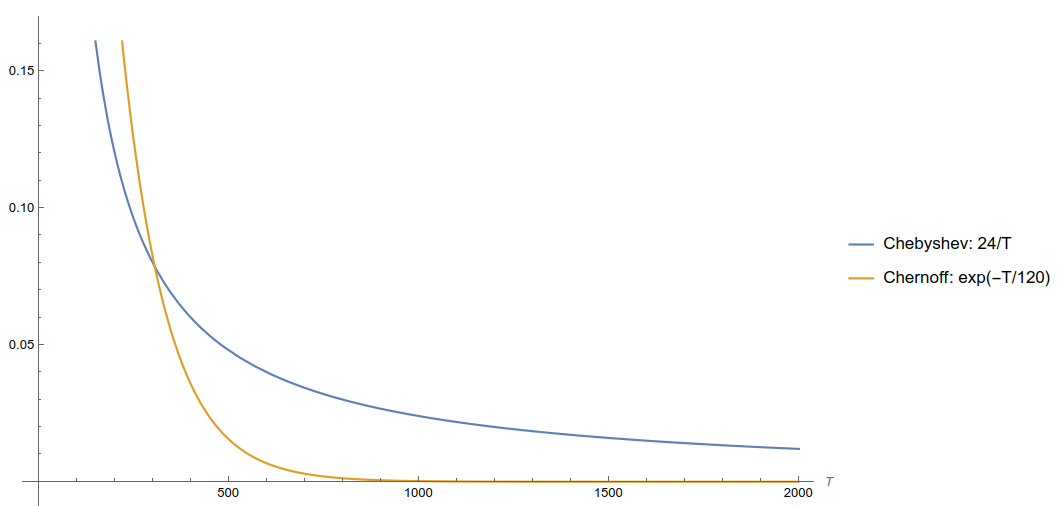
\includegraphics[width=1.25\textwidth]{figures/fig-chernoff-v-chebyshev.png}
    \caption{Bounds on $\bPr{ Y < \frac{1}{2}T }$ provided by Chebyshev's and Chernoff's inequalities, as a function of $T$.}
    \label{fig:chernoff:v:chebyshev}
\end{figure}
In any case: we wanted a failure probability less than $\errprob$? Then is suffices to solve for (integer) $T$:
\[
e^{-\frac{1}{120}T} \leq \errprob
\]
giving $T \geq \clg{120\ln(1/\errprob)}$. So with taking $T(\errprob)=O(\log(1/\errprob))$ in~\cref{algo:majority:vote} suffices to amplify the success probability of each query on $\blue{x}$ from $60\%$ to $1-\errprob$, at the (small?) cost of $O(\log(1/\errprob))$ more queries to the data structure $\red{D}$.

\begin{framed}
 We have used Markov's and Chebyshev's inequalities and the Chernoff bound, and this allowed us to analyse and amplify the success probability of our randomised algorithms. In the next lectures, we will see a related technique, also based on the Chernoff (or, looking ahead, Hoeffding) bound: a generalisation of the ``majority vote'' trick for when the output can take more than only 2 values, called the \emph{median trick.}
\end{framed}


\section{Concentration inequalities: a summary}
We summarize the ``concentration bounds''\marginnote{They are called that way because they quantify how ``concentrated'' (in terms of probability) a random variable is around its expectation.} used in the chapter so far, along with some others (more advanced) that will come in handy in the next chapters. These will be sufficient in many or most settings. 
There are, of course, \emph{many} others, and many refinements or variants of the bounds we present here. If you are interested, see \eg Chapter~2 of \cite{Vershynin18} or~\cite{BoucheronLM13} for a much more comprehensive and insightful coverage.

We start with the mother of all concentration inequalities, Markov's inequality:
\begin{theorem}[Markov's inequality]
  \label{theo:markov}
Let $X$ be a non-negative random variable with $\bEE{X} < \infty$. For any $t > 0$, we have
\[  
  \bPr{ X \geq t } \leq \frac{\bEE{X}}{t}
\]
\end{theorem}
\noindent Applying this to $(X-\bEE{X})^2$, we get 
\begin{theorem}[Chebyshev's inequality]
  \label{theo:chebyshev}
Let $X$ be a random variable with $\bEE{X^2} < \infty$. For any $t > 0$, we have
\[  
  \bPr{ \abs{X-\bEE{X}} \geq t } \leq \frac{\var[X]}{t^2}
\]
\end{theorem}
By applying Markov's inequality to the moment-generating function (MGF) of $\sum_{i=1}^n X_i$ in various ways, one can also obtain the following statements:
\begin{theorem}[Hoeffding bound]
  \label{theo:hoeffding}
Let $X_1,\dots,X_n$ be independent random variables, where $X_i$ takes values in $[a_i,b_i]$. For any $t \geq 0$, we have
\begin{align}
\bPr{ \sum_{i=1}^n X_i   > \sum_{i=1}^n \bEE{X_i} + t }  
&\leq \exp(-\frac{2 t^2}{\sum_{i=1}^n (b_i-a_i)^2}) \\
\bPr{\sum_{i=1}^n X_i  < \sum_{i=1}^n \bEE{X_i} - t }
 &\leq \exp(-\frac{2 t^2}{\sum_{i=1}^n (b_i-a_i)^2})
 \end{align}
\end{theorem}

\begin{corollary}[Hoeffding bound]
  \label{coro:hoeffding}
Let $X_1,\dots,X_n$ be \iid random variables taking value in $[0,1]$, with mean $\mu$. For any $\gamma \in (0,1]$ we have
\begin{align}
\bPr{ \abs{\frac{1}{n}\sum_{i=1}^n X_i  - \mu} > \gamma }
 &\leq 2\exp(-2 \gamma^2 n)
\end{align}
\end{corollary}

\begin{theorem}[Chernoff bound]
  \label{theo:chernoff}
Let $X_1,\dots,X_n$ be independent random variables taking value in $[0,1]$, and let $P \eqdef \sum_{i=1}^n \bEE{X_i}$ For any $\gamma \in (0,1]$ we have
\begin{align}
\bPr{\sum_{i=1}^n X_i > (1+\gamma)P } &< \exp(-\gamma^2 P/3)\\
\bPr{\sum_{i=1}^n X_i < (1-\gamma)P } &< \exp(-\gamma^2 P/2)
\end{align}
In particular, if $X_1,\dots,X_n$ are \iid with mean $\mu$, then for any $\gamma \in (0,1]$ we have
\begin{align}
\bPr{ \abs{\frac{1}{n}\sum_{i=1}^n X_i  - \mu} > \gamma\mu }
 &\leq 2\exp(-\gamma^2 n \mu/3) \label{eq:chernoff:iid}
\end{align}
\end{theorem}
As a rule of thumb, the ``multiplicative'' (Chernoff) from~\cref{theo:chernoff} is preferable to the ``additive'' bound (Hoeffding) from~\cref{coro:hoeffding} whenever $\mu  \eqdef P/n \ll 1$. In case one only has an upper or lower bound on the quantity $P = \sum_{i=1}^n \bEE{X_i}$, the following version of the Chernoff bound can come in handy:
\begin{theorem}[Chernoff bound (upper and lower bound version)]
  \label{theo:chernoff:with:ublb}
In the setting of~\cref{theo:chernoff}, suppose that
$P_L \leq P \leq P_H.$ Then for any $\gamma \in (0,1]$, we have
\begin{align}
\bPr{\sum_{i=1}^n X_i > (1+\gamma)P_H } &< \exp(-\gamma^2 P_H/3) \\
\bPr{\sum_{i=1}^n X_i < (1-\gamma)P_L } &< \exp(-\gamma^2 P_L/2)
\end{align}
\end{theorem}

%%%%%%%%%%%%%%%%%%%%%%%%%%%%%%%%%%%%%%%%%%%%%%%%%%%%%%%%%%%%%%%
\iffalse
\begin{theorem}[Bernstein's inequality] \label{theo:bernstein}
	Let $X_1,\dots, X_n$ be independent random variables taking values in $[-a,a]$, and such that $\bEE{X_i^2} \leq v_i$ for all $i$. Then, for every $t\geq 0$, we have
	\[
	\bPr{ \abs{\sum_{i=1}^n X_i-\sum_{i=1}^n \bEE{X_i}} \geq t } \leq \exp\Paren{-\frac{t^2}{2(\sum_{i=1}^n v_i+\frac{a}{3}t)}}\,.
	\]
	In particular, if $X_1,\dots,X_n$ are \iid with mean $\mu$ and $\bEE{X_1^2} \leq v$, then for any $\gamma \geq 0$ we have
	\[
	\bPr{ \abs{\frac{1}{n}\sum_{i=1}^n X_i-\mu} \geq \gamma } \leq \exp\Paren{-\frac{\gamma^2n}{2(v+\frac{a}{3}\gamma)}}\,.
	\]
\end{theorem}
Observe that this tail bound exhibits both behaviours: it decays in a subgaussian fashion for small $\gamma$, before switching to a subexponential tail bound for large $\gamma$. 

We conclude this section by providing a very convenient bound, specifically for Poisson random variables, which shares the same ``two-tail'' behaviour:
\begin{theorem}[Poisson concentration]\label{theo:main:poisson:bounds}
Let $X$ be a $\poisson{\lambda}$ random variable, where $\lambda > 0$. Then, for any $t>0$, we have
\begin{equation}\label{eq:poisson:upper:tail}
    \probaOf{ X \geq \lambda + t} \leq e^{-\frac{t^2}{2\lambda}\psi\Paren{\frac{t}{\lambda}}} \leq e^{-\frac{t^2}{2(\lambda+t)}}
\end{equation}
and, for any $0<t< \lambda$,
\begin{equation}\label{eq:poisson:lower:tail}
  \probaOf{ X \leq \lambda - t} \leq e^{-\frac{t^2}{2\lambda}\psi\Paren{-\frac{t}{\lambda}}} \leq e^{-\frac{t^2}{2(\lambda+t)}}\,,
\end{equation}
where $\psi(u)\eqdef 2\frac{(1+u)\ln(1+u)-u}{u^2}$ for $u\geq -1$.
In particular, for any $t\geq 0$,
\begin{equation}\label{eq:poisson:both:tail}
  \probaOf{ \abs{X -\lambda} \geq t} \leq 2e^{-\frac{t^2}{2(\lambda+t)}}\,.
\end{equation}
\end{theorem}
\cmargin{Is the proof needed?}
\fi

\chapter{Lecture 3: Balls in Bins}
You have $\nballs$ balls, and want to randomly distribute them among $\nbins$ different bins. Why? That's a pretty good question: basically, and you'll have to believe me for now, this rather strange scenario (and its many variants) capture a lot of actual interesting or well-motivated problems.\marginnote{We'll get back to those.}

The things we might care about are (1)~the \emph{maximum load} of the bins, that is, what's the maximum number of balls any given bin contains once we've distributed them; (2)~the \emph{coverage}, that is, how many bins are non-empty; and (3)~the \emph{collisions}, that is, how many pairs of distinct balls share the same bin.

The simplest thing we can do is throwing our $\nballs$ into the $\nbins$ independently and uniformly at random. Let's see how that goes.

\section{Collisions}
One of the most basic things we can ask is whether the $\nballs$ balls will all fall into their own personal bin, that is, if there's going to be at least one bin containing more than one ball. \emph{What's the probability to get at least one collision?}

\paragraph{Interlude:} \emph{run the Birthday Paradox experiment in the classroom. Discuss assumptions (uniformity), etc.}

\begin{theorem}[Birthday Paradox]
If you gather 23 people in a room, then with probability 50\% there will be two sharing a birthday.
\end{theorem}

To prove that, we'll tackle the more general question, for arbitrary $\nballs$ and $\nbins$, of finding what the probability $p_{\nballs, \nbins}$ of having at least one collision is: the birthday paradox is for $\nbins=366$, because, of course, 2024 is a leap year\marginnote{That might change in 2025...}, and asks to check that $p_{23,366} \geq 1/2$. Now, the result has to depend on the relation between $\nballs$ and $\nbins$: if $\nballs \geq \nbins + 1$, then that probability is exactly one,\marginnote{Do you see why? Prove it (Pigeonhole).} while if $\nbins \gg \nballs$ this should be less likely.

\begin{theorem}
    \label{theo:collisions:pnm}
    The probability $p_{\nballs, \nbins}$ to get at least one collision is equal to
    \begin{equation}
        \label{eq:collisions:pnm}
        p_{\nballs, \nbins} = 1 - \frac{\nbins!}{\nbins^{\nballs}(\nbins-\nballs)!} = 1 - \frac{\nballs!}{\nbins^{\nballs}} \binom{\nbins}{\nballs}
    \end{equation}
    In particular, for $\nballs = 23$ and $\nbins=366$, this is...?\marginnote{Check it: $p_{22,366} \approx 0.475$, while $p_{23,366} \approx 0.506$.}
\end{theorem}
\begin{proof}
    \begin{align*}
    1-p_{\nballs, \nbins} &= \frac{\nbins}{\nbins}\cdot\frac{\nbins-1}{\nbins}\cdot \frac{\nbins-2}{\nbins}\cdots \frac{\nbins-\nballs+1}{\nbins}
    = \frac{1}{\nbins^{\nballs}}\prod_{\ell=0}^{\nballs-1} (\nbins-\ell) \\
    &= \frac{\nbins!}{\nbins^{\nballs}(\nbins-\nballs)!} 
    \end{align*}
\end{proof}
\begin{figure}[htbp]
    \centering
    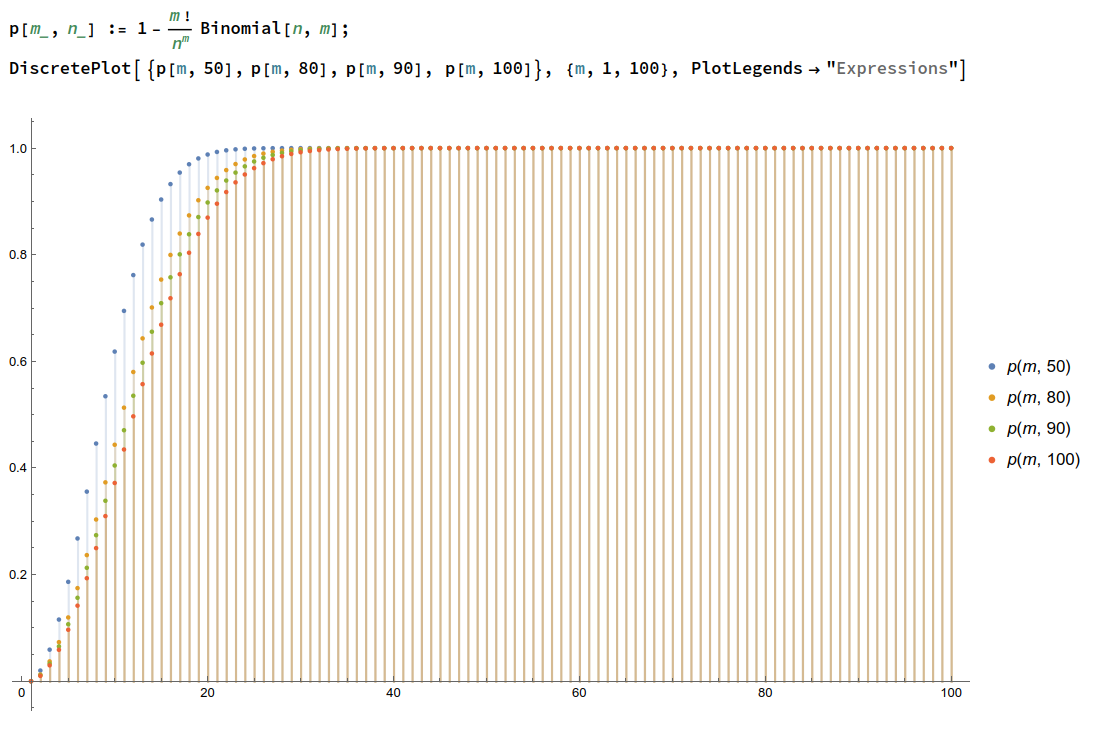
\includegraphics[width=1.0\textwidth]{figures/fig-collisions-nm.png}
    \caption{The quantity $p_{\nballs, \nbins}$ from~\cref{eq:collisions:pnm}, plotted here as a function of $\nballs$ for various choices of $\nbins$.}
    \label{fig:collisions:nm}
\end{figure}

Looking at the graph above, it looks like we approach a very high probability of getting a collision \emph{way} before $\nballs = \Theta(\nbins)$. Any guess at what $\nballs$ should be to, say, have probability at least $50\%$ of a collision? Should it be
\begin{itemize}
    \item $\Theta(\log\nbins)$?
    \item $\Theta(\sqrt{\nbins})$?
    \item $\Theta\Paren{\frac{\nbins}{\log\nbins}}$?
    \item Something else?
\end{itemize}
And \emph{why}?

\paragraph{The worst approach: rabbit-out-of-a-hat, no intuition given.} Take $\nballs = c\cdot\sqrt{\nbins}$ for some fixed constant $c>0$. Plugging this in the expression $p_{\nballs,\nbins}$ obtained in~\cref{theo:collisions:pnm}, we get
\begin{align*}
1 - p_{\nballs,\nbins} = \frac{\nbins!}{\nbins^{\nballs}(\nbins-\nballs)!}
&\operatorname*{\sim}_{\nbins\to\infty} 
\frac{1}{\nbins^{\nballs}}\cdot \frac{\sqrt{2\pi \nbins} \Paren{\frac{\nbins}{e}}^{\nbins}}{\sqrt{2\pi(\nbins-\nballs)}\Paren{\frac{\nbins-\nballs}{e}}^{\nbins-\nballs}} \tag{Stirling} \\
&= \frac{1}{\sqrt{1-\frac{\nballs}{\nbins}}} \frac{ \nbins^{\nbins-\nballs}}{\Paren{\nbins-\nballs}^{\nbins-\nballs} e^{\nballs}} \tag{``Massaging''}\\
&= \frac{1}{\sqrt{1-\frac{\nballs}{\nbins}}} \frac{1}{\Paren{1-\frac{\nballs}{\nbins}}^{\nbins-\nballs} e^{\nballs}} \\
&= \frac{1}{\sqrt{1-\frac{\nballs}{\nbins}}} \frac{1}{\Paren{1-\frac{\nballs}{\nbins}}^{\nbins} e^{\nballs}} \cdot \Paren{1-\frac{\nballs}{\nbins}}^{\nballs} \\
&= \frac{1}{\sqrt{1-\frac{c}{\sqrt{\nbins}}}} \frac{1}{\Paren{\Paren{1-\frac{c}{\sqrt{\nbins}}}^{\sqrt{\nbins}} e^{c}}^{\sqrt{\nbins}}} \cdot \Paren{1-\frac{c}{\sqrt{\nbins}}}^{c\sqrt{\nbins}} \tag{Finally!}
\end{align*}
the last line using our choice of $\nballs$. From there, ``all'' that remains to check is that $\lim_{\nbins\to\infty} \sqrt{1-\frac{c}{\sqrt{\nbins}}} = 1$ (easy), that 
\[
\lim_{\nbins\to\infty} \Paren{\Paren{1-\frac{c}{\sqrt{\nbins}}}^{\sqrt{\nbins}} e^{c}}^{\sqrt{\nbins}} = e^{-c^2/2}
\] (less easy)\marginnote{Do it!}, and that
\[
\lim_{\nbins\to\infty} \Paren{1-\frac{c}{\sqrt{\nbins}}}^{c\sqrt{\nbins}} = e^{-c^2}
\]
(not too hard?) to conclude that
\begin{align*}
1 - p_{c\sqrt{\nbins},\nbins} 
&\operatorname*{\sim}_{\nbins\to\infty} 1\cdot \frac{1}{e^{-c^2/2}} \cdot e^{-c^2} = e^{-c^2/2} 
\end{align*}
or, equivalently,
\begin{align*}
p_{c\sqrt{\nbins},\nbins} 
= 1 - e^{-c^2/2} +o(1)
\end{align*}
This shows that the probability to get a collision becomes constant for $\nballs = \Theta(\sqrt{\nbins})$.
Now, that's nice, but you may ask yourself, \emph{``Well, how did I get here?''}

\paragraph{Let's take a step back.} So we throw $\nballs$ balls into $\nbins$ bins. Let's start with the simplest case possible: let's throw \emph{two} balls into $\nbins$. What's the probability that they end up in the same bin?\marginnote{Don't look immediately! Think about it first.}\clearpage

The first ball falls into a given bin, say the $i$-th. Then to get a collision the second ball has to be thrown into the same bin $i$, which happens with probability $1/\nbins$. So $p_{2,\nbins} = 1/\nbins$. A more verbose way to derive it is as follows: let $\red{X_1}, \blue{X_2}$ denote the indices of the bins $\bin$ for the first $\balla$ and second $\ballb$ ball, respectively. These are independent r.v.'s, uniformly distributed in $[\nbins]$, so
\begin{align}
p_{2,\nbins} &= \probaOf{\red{X_1}=\blue{X_2}} = \sum_{k=1}^{\nbins} \probaOf{\red{X_1}=k, \blue{X_2}=k} \notag\\
&= \sum_{k=1}^{\nbins} \probaOf{\red{X_1}=k}\cdot\probaOf{\blue{X_2}=k} \notag\\
&= \sum_{k=1}^{\nbins} \frac{1}{\nbins}\cdot\frac{1}{\nbins} = \frac{\nbins}{\nbins^2} = \frac{1}{\nbins} \,,
\end{align}
``as foretold.''

Back to the general $\nballs$ balls case. The above tells us that for every pair of balls, the probability to get a collision (ignoring all other balls) is $1/\nbins$. How many distinct pairs of balls do we have? Well, $\binom{\nballs}{2}$. So what's the \emph{expected} number of collisions $c(\nballs,\nbins)$?
\begin{align}
   c(\nballs,\nbins) 
   &= \expect{\sum_{(\red{i},\blue{j})\text{ pair}} \indic{\red{X_i} = \blue{X_j}} }\notag\\
   &= \sum_{(\red{i},\blue{j})\text{ pair}} \expect{\indic{\red{X_i} = \blue{X_j}} }\notag\\
   &= \sum_{(\red{i},\blue{j})\text{ pair}} \probaOf{\red{X_i} = \blue{X_j}} \notag\\
   &= \sum_{(\red{i},\blue{j})\text{ pair}} \frac{1}{\nbins} \notag\\
   &= \binom{\nballs}{2}\cdot\frac{1}{\nbins} \label{eq:expect:collisions}
\end{align}
where we used linearity of expectation, and our previous computation for the $\nballs=2$ case. This means that the expected number of collisions grows (roughly) as $\frac{\nballs^2}{2\nbins}$. If we believe that the number of collisions does not deviate too pathologically from its expected value, this becomes constant when $\nballs = \bigTheta{\sqrt{\nbins}}$. So we should start expecting collisions when $\nballs = \bigTheta{\sqrt{\nbins}}$, which explains (in hindsight) the result we got before!

But can we easily prove this ``intuition''? We have the expectation $c(\nballs,\nbins)$ of the number of collisions, we want to show that number (let's call this random variable $C$) does not deviate too far from its expectation. The most basic tools we've seen for this are Markov and Chebyshev's inequalities: here, we'll have to use Chebyshev.\marginnote{Do you see why?} So we need to compute the variance of our random variable $C$:
\[
C = \sum_{(\red{i},\blue{j})\text{ pair}} \indic{\red{X_i} = \blue{X_j}}
\]
where as before \red{$X_i$} is the index of the bin \bin where the \red{$i$}-th ball \ball lands, and $\indic{\red{X_i} = \blue{X_j}}$ is the indicator of the event \emph{``ball $\red{i}$ and ball $\red{j}$ collide.''}
We \emph{would like} to write that the variance of the sum is the sum of the variances (``linearity of variance''), something like this
\begin{align*}
\var[C] 
&= \var\left[\sum_{(\red{i},\blue{j})\text{ pair}} \indic{\red{X_i} = \blue{X_j}}\right] 
\stackrel{?}{=} \sum_{(\red{i},\blue{j})\text{ pair}} \var\left[\indic{\red{X_i} = \blue{X_j}}\right] \\
\end{align*}
which \emph{would} make our life so much easier, since then, using the variance of an indicator random variable (Bernoulli), we'd get
\[
\var[C] = \binom{\nballs}{2}\frac{1}{\nbins}\Paren{1-\frac{1}{\nbins}}
\]
Unfortunately, \emph{variance is not linear}: we could write the above $\stackrel{?}{=}$ equality \emph{if} the indicator variables $\indic{\red{X_i} = \blue{X_j}}$ were independent (across $(\red{i},\blue{j})$): \emph{and this is not the case here}.\marginnote{Do you see why they are not independent?}

And yet, since we are showing the bin (for each ball) \emph{uniformly} at random, some magic happens, and somehow the above expression is still true.\marginnote{In the proof below, locate exactly where we use the fact that the bin is chosen uniformly.}
\begin{lemma}[Well, actually\dots \advancedstuff]
\label{lemma:variance:collisions}
We have 
\[
\var[C] = \binom{\nballs}{2}\frac{1}{\nbins}\Paren{1-\frac{1}{\nbins}}
\]
\end{lemma}
\begin{proof}
    Since $\var[C] = \bEE{C^2} - \bEE{C}^2$ and we already have computed $\bEE{C}$, we only are missing the first term:
    \begin{align*}
        \bEE{C^2} &= \bEE{\left(\sum_{(\red{i},\blue{j})\text{ pair}} \indic{\red{X_i} = \blue{X_j}}\right)^2} \\
        &= \bEE{\sum_{(\red{i},\blue{j})\text{ pair}}\sum_{(\orange{k},\green{\ell})\text{ pair}} \indic{\red{X_i} = \blue{X_j}}\indic{\orange{X_k} = \green{X_\ell}}} \\
        &= \sum_{(\red{i},\blue{j})\text{ pair}}\sum_{(\orange{k},\green{\ell})\text{ pair}} \bEE{\indic{\red{X_i} = \blue{X_j}}\indic{\orange{X_k} = \green{X_\ell}}} \\
    \end{align*}
    This is a little intimidating to compute, but we can make the following observations about the summands:
    \begin{itemize}
        \item if the two pairs $(\red{i},\blue{j})$, $(\orange{k},\green{\ell})$ are the same,\footnote{When we consider pairs here, we don't care about ordering, so $(i,j)=(j,i)$.} then $\indic{\red{X_i} = \blue{X_j}}\indic{\orange{X_k} = \green{X_\ell}} = \indic{\red{X_i} = \blue{X_j}}^2 = \indic{\red{X_i} = \blue{X_j}}$, so
        \[
            \bEE{\indic{\red{X_i} = \blue{X_j}}\indic{\orange{X_k} = \green{X_\ell}}} 
            = \bEE{\indic{\red{X_i} = \blue{X_j}}} 
            = \frac{1}{\nbins}\,.
        \]
        There are exactly $\binom{\nballs}{2}$ such summands.
        \item if the two pairs $(\red{i},\blue{j})$, $(\orange{k},\green{\ell})$ are disjoint, then $\indic{\red{X_i} = \blue{X_j}}$, $\indic{\orange{X_k} = \green{X_\ell}}$ are independent, and so
        \[
            \bEE{\indic{\red{X_i} = \blue{X_j}}\indic{\orange{X_k} = \green{X_\ell}}} 
            = \bEE{\indic{\red{X_i} = \blue{X_j}}} \bEE{\indic{\orange{X_k} = \green{X_\ell}}} 
            = \frac{1}{\nbins^2}\,.
        \]
        There are exactly $\binom{\nballs}{2}\binom{\nballs-2}{2}$ such summands.
        \item else, then the two pairs $(\red{i},\blue{j})$, $(\orange{k},\green{\ell})$ are neither disjoint nor equal, then $|\{\red{i},\blue{j},\orange{k},\green{\ell}\}|=3$. For any such summand, $\indic{\red{X_i} = \blue{X_j}}\indic{\orange{X_k} = \green{X_\ell}}$ is of the form $\indic{\red{X_i} = \blue{X_j} = \orange{X_k}}$, and so
        \begin{align*}
            \bEE{\indic{\red{X_i} = \blue{X_j}}\indic{\orange{X_k} = \green{X_\ell}}} 
            &= \bEE{\indic{\red{X_i} = \blue{X_j} = \orange{X_k}}} \\
            &= \sum_{b=1}^{\nbins} \probaOf{\red{X_i} = b,  \blue{X_j} = b, \orange{X_k} = b} \\
            &= \frac{\nbins}{\nbins^3}\\
            &= \frac{1}{\nbins^2}\,.
        \end{align*}
        There are exactly $2\cdot \binom{3}{2}\binom{\nballs}{3} = 6\binom{\nballs}{3}$ such summands.\marginnote{Can you see why? (If that's any consolation, I am terrible at combinatorics.)}
    \end{itemize}
    As a sanity check, we do have $\binom{\nballs}{2} + \binom{\nballs}{2}\binom{\nballs-2}{2} + 6\binom{\nballs}{3} = \binom{\nballs}{2}^2$, so we did not miss any summand in the above distinction of cases. We can then rewrite
    \begin{align*}
        \bEE{C^2} 
        &= \binom{\nballs}{2}\cdot \frac{1}{\nbins}
        + \binom{\nballs}{2}\binom{\nballs-2}{2}\cdot \frac{1}{\nbins^2}
        + 6\binom{\nballs}{3}\cdot \frac{1}{\nbins^2} \\
        &= \binom{\nballs}{2}\cdot \frac{1}{\nbins} + \binom{\nballs}{2}^2\cdot \frac{1}{\nbins^2} - \binom{\nballs}{2}\cdot \frac{1}{\nbins^2} \tag{Magic?} \\
        &= \binom{\nballs}{2}\cdot \frac{1}{\nbins}\Paren{1-\frac{1}{\nbins}} + \binom{\nballs}{2}^2\cdot \frac{1}{\nbins^2} 
    \end{align*}
    That's really encouraging, since the second term is exactly $\bEE{C}^2$, and the first is what we were hoping to get for the variance. And, indeed:
    \begin{align*}
        \var[C] &= \bEE{C^2} - \bEE{C}^2
        = \binom{\nballs}{2}\frac{1}{\nbins}\Paren{1-\frac{1}{\nbins}} + \binom{\nballs}{2}^2 \frac{1}{\nbins^2}  - \Paren{\binom{\nballs}{2} \frac{1}{\nbins}}^2 \\
        &= \binom{\nballs}{2} \frac{1}{\nbins}\Paren{1-\frac{1}{\nbins}}\,,
    \end{align*}
    concluding the proof.
\end{proof}
\begin{framed}
Here, we were lucky: somehow in the variance calculation some terms ``magically cancel out'' and we get the same expression as if things were independent. \emph{This is not usually the case!} But there are some `ways to handle things nonetheless. For instance:
\begin{itemize}
    \item If $X_1,\dots,X_n$ are \emph{negatively correlated}, then 
    \[
    \var[\sum_{i=1}^n X_i] \leq \sum_{i=1}^n \var[X_i]
    \]
    \item Since $\var[X] = \expect{X^2} - \expect{X}^2$, we can always write
    \[
    \var[X] \leq \expect{X^2}\,.
    \]
    Sometimes, it's good enough!
\end{itemize}  
\end{framed}\marginnote{There are also other ``fancier'' ways, such as the Efron--Stein inequality, but that's slightly out of scope. Check it out if interested!}  

Now we have the expectation (\cref{eq:expect:collisions}), we have the variance (\cref{lemma:variance:collisions}), and we have Chebyshev. For any $t>0$,
\[
\probaOf{|C - c(\nballs,\nbins)| \geq t} \leq \frac{\var[C]}{t^2} \leq \frac{c(\nballs,\nbins)}{t^2}
\]
Let's set $\nballs = \flr{3\sqrt{\nbins}}$, so that (using $\nbins \geq 2$)
\[
c(\nballs,\nbins) = \binom{\flr{3\sqrt{\nbins}}}{2}\cdot\frac{1}{\nbins} \geq 2
\]
(it's not immediate, but can be checked); and $t \eqdef c(\nballs,\nbins)$. We then have
\[
\probaOf{C=0} \leq \probaOf{|C - c(\nballs,\nbins)| \geq c(\nballs,\nbins)} \leq \frac{1}{c(\nballs,\nbins)} \leq \frac{1}{2}
\]
showing that \emph{we have at least a 50\% chance to get a collision as soon as $\nballs \geq \flr{3\sqrt{\nbins}}$.} And conversely, using this time Markov's inequality,\marginnote{This inequality, $\probaOf{X=0} \geq 1-\expect{X}$ for $X$ integer-valued, is sometimes referred to as the \emph{first moment method}.}
\[
\probaOf{C\neq 0} = \probaOf{C\geq 1}  \leq \expect{C} = c(\nballs,\nbins) \leq \frac{\nballs^2}{2\nbins}
\]
which is less than $50\%$ for $\nballs \leq \flr{\sqrt{\nbins}}$. To sum up, we proved, using Chebyshev's and Markov's inequalities:
\begin{theorem}
    The probability to get \emph{at least one collision} when throwing $\nballs$ independent and uniformly at random in $\nbins$ bins is less than $1/2$ when $\nballs \leq \flr{\sqrt{\nbins}}$, and at least $1/2$ as soon as $\nballs \geq \flr{\sqrt{3\nbins}}$.
\end{theorem}
\noindent confirming the empirical observations and (hopefully) gaining some intuition along the way.

\subsection{Applications}

\begin{itemize}
    \item Hashing, and hash functions
    \item Distribution testing (statistics)
    \item Lower bounds for other problems!
\end{itemize}

\section{Coverage}
Another very natural thing to ask is \emph{when each bin will have received at least one ball}. This is often referred to as the \emph{coupon collector} problem, a term coined a long time ago, when computer scientists were eating cereals for breakfast hoping to collect all of the coupons (cards) of a collection, one cereal box at a time.\marginnote{We will stick with the balls-and-bins scenario. But yes, gotta catch'em all!}

Obviously, since we are trying to hit at least each of $\nbins$ bins at least once, we need to throw at least $\nballs \geq \nbins$ balls. But is it enough?
\begin{framed}
    \noindent What is the expected number of balls $\green{M}(\nbins)$ one needs to throw before each of the $\nbins$ bins contains at least one of the $\nballs$ balls?
\end{framed}
To figure it out, we can start by trying to simulate the experiment.\marginnote{This code is definitely \emph{not} optimised!}
\begin{lstlisting}
import numpy as np
import random
def coverage(n):
    (m,ncovered) = (0,0)
    covered = np.zeros(n)
    while ncovered < n:
        draw = random.randint(1, n);
        if covered[draw-1] == 0:
            covered[draw-1] = 1
            ncovered += 1
        m += 1
    return m
\end{lstlisting}
\begin{lstlisting}
list_n = np.arange(10, 1001);
experiments_avg = np.zeros(np.size(list_n));
experiments_std = np.zeros(np.size(list_n));
for i in range(len(list_n)):
    coverages_trials = [coverage(list_n[i]) for _ in range(100)];
    experiments_avg[i] = np.mean(coverages_trials);
    experiments_std[i] = np.std(coverages_trials);
\end{lstlisting}
\begin{figure}[htbp]\centering
    \label{fig:coverage:1}
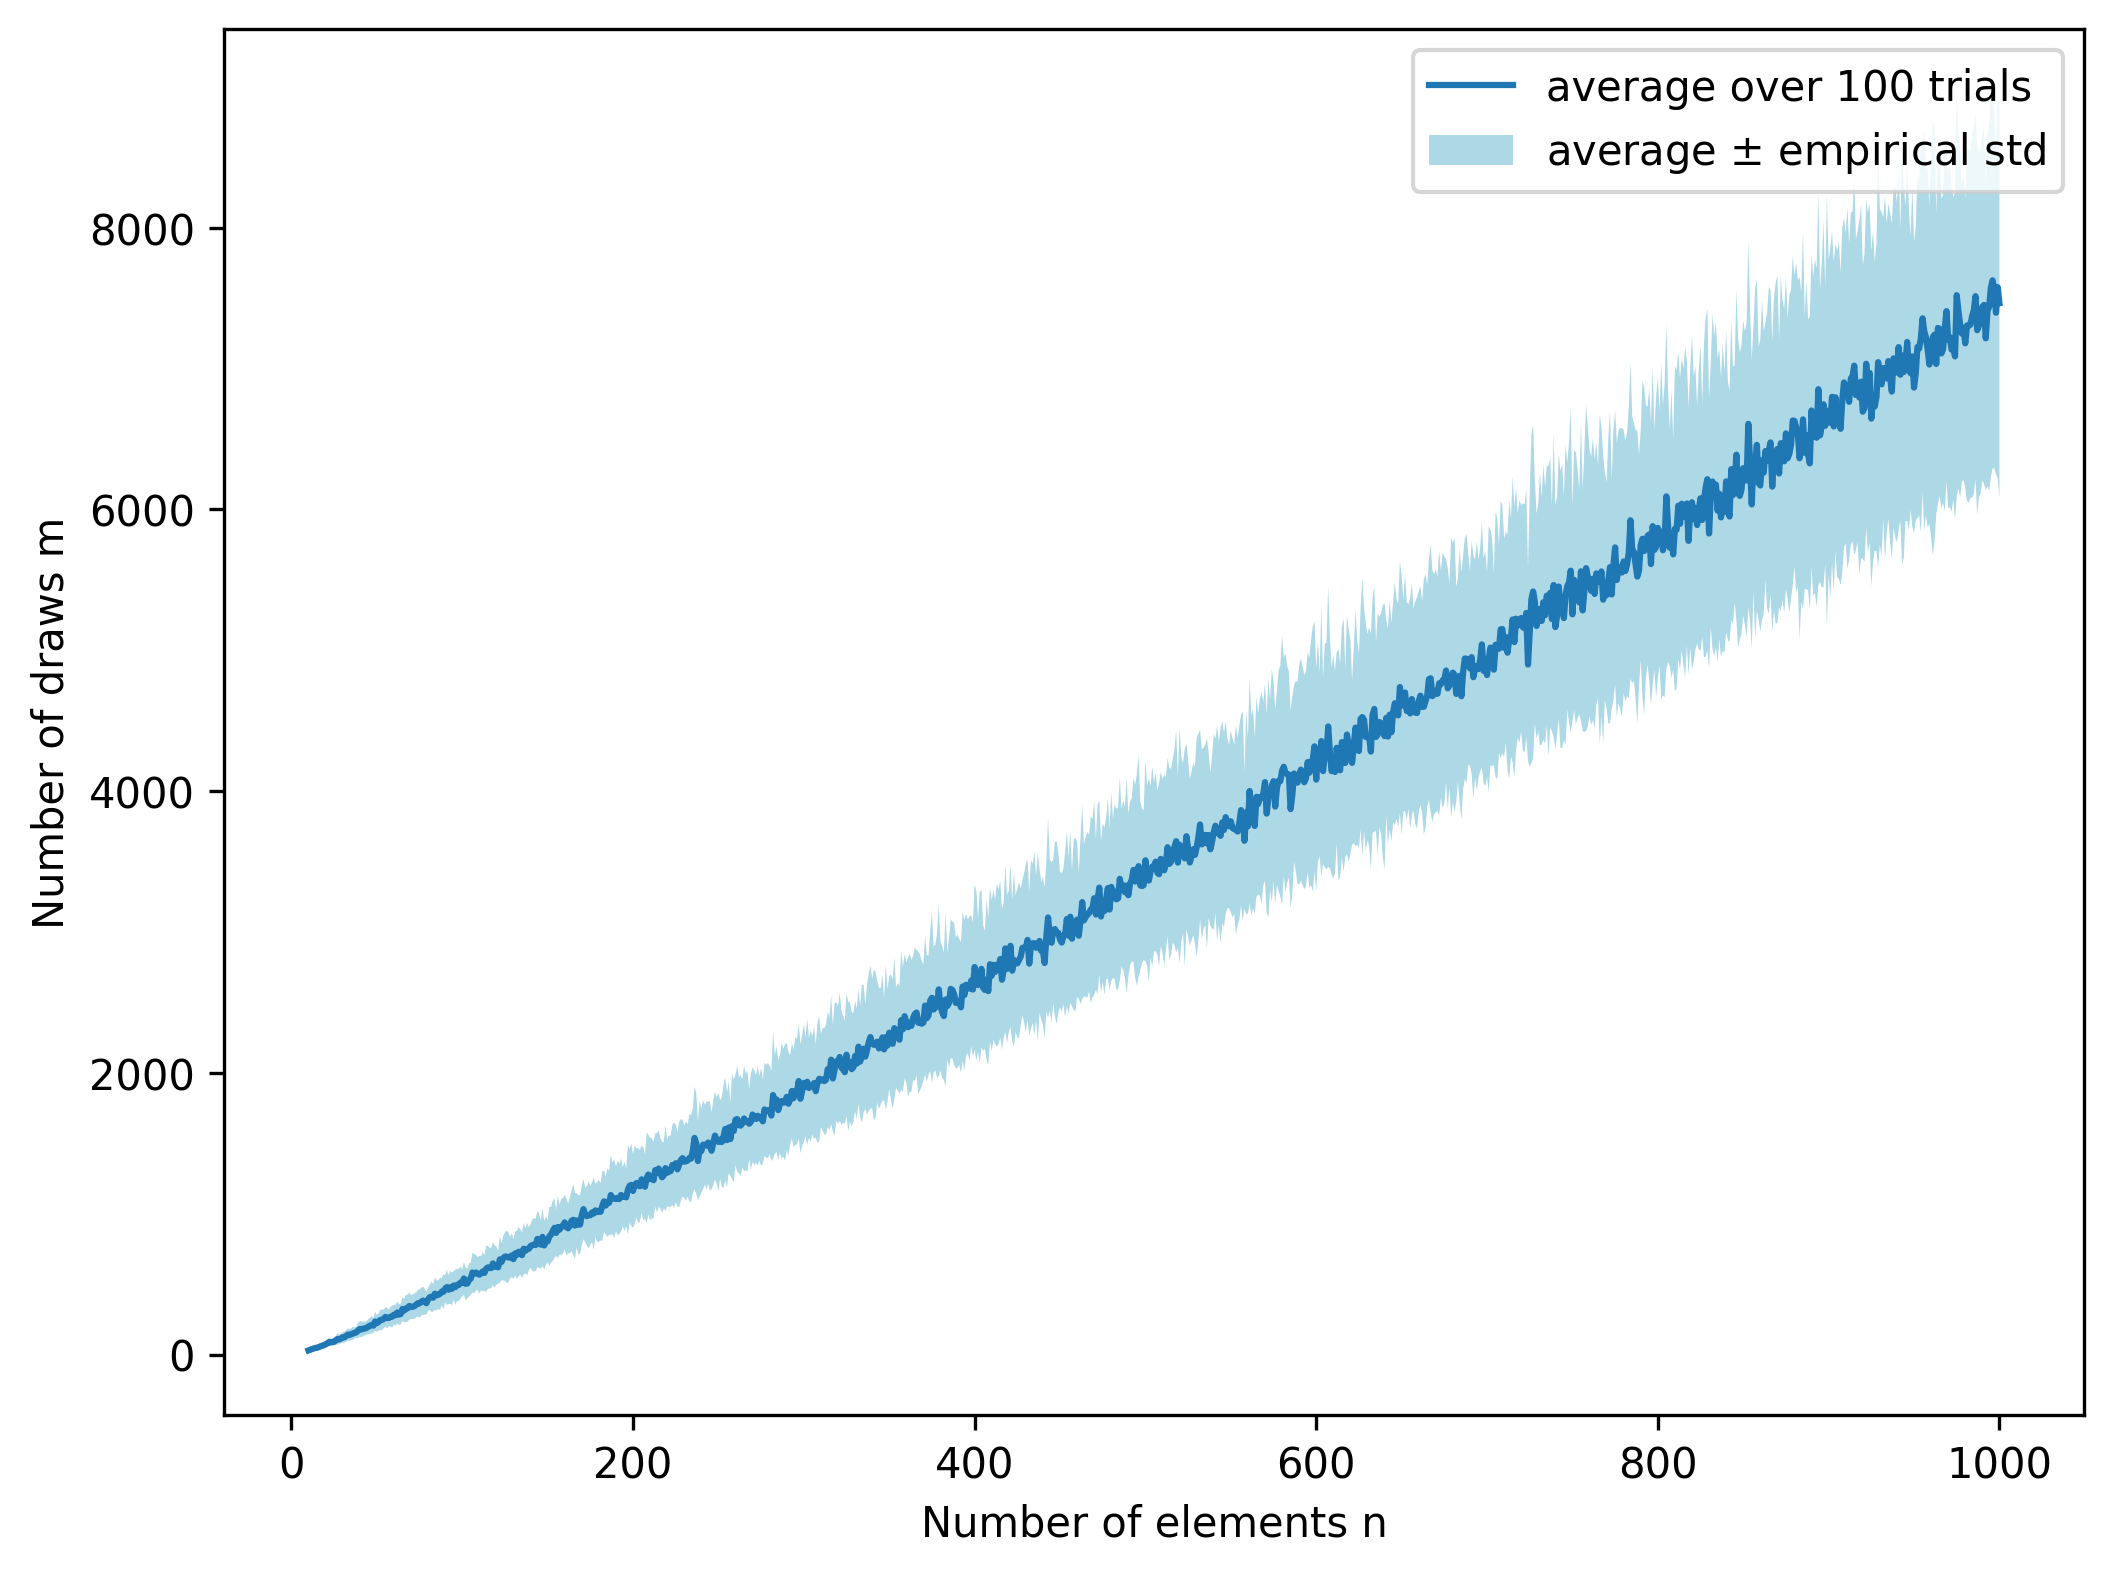
\includegraphics[width=0.9\textwidth]{figures/fig-coverage1.png}
\caption{Average (over 100 trials) of the number of balls thrown until all of the $\nbins$ bins contain at least one ball, as a function of $\nbins$. The range given by one empirical standard deviation is plotted alongside.}
\end{figure}

Looking at the graph above, we can see how the average number of balls to throw grows with $\nbins$. But what is it, quantitatively? How does $\green{M}(\nbins)$ behaves?
\begin{itemize}
    \item $\Theta(\nbins)$?
    \item $\Theta(\nbins\log\nbins)$?
    \item $\Theta(\nbins^{3/2})$?
    \item Something else?
\end{itemize}
And \emph{why}?

\paragraph{Some intuition.} Let's look at what happens when $\nballs=\nbins$: how many bins \emph{haven't} been hit by a balls when we have thrown $\nbins$ of them. The probability a fixed bin does not contain any ball is
\[
\Paren{1-\frac{1}{\nbins}}^{\nbins} \approx e^{-1}
\]
and so the expected number of bins with no balls, by linearity of expectation, is
\begin{equation}
    \label{eq:expected:empty:bins}
\expect{\text{empty bins after }\nbins\text{  balls}}=\sum_{i=1}^{\nbins} \probaOf{\substack{\text{bin $i$ empty}\\\text{ after }\nbins\text{  balls}}} =\nbins\cdot \Paren{1-\frac{1}{\nbins}}^{\nbins} \approx \frac{\nbins}{e}
\end{equation}
This means that after throwing $\nbins$ balls, we still have a constant fraction ($\approx 1/e$) of bins to still hit. Repeating the argument, if we throw $\nbins$ more balls, we expect to still have $\approx 1/e^2$ empty bins; $\nbins$ more balls, and the remaining fraction will be $\approx1/e^3$; etc. Each time we throw $\nbins$ more balls, we decrease (in expectation) the number of empty bins by a constant factor, so\dots{} to bring the expected number of empty bins to $<1$, we'll need to repeat that $\Theta(\log\nbins)$ times.\marginnote{Generalise~\cref{eq:expected:empty:bins} to $\nballs$ bins, to compute directly \[\expect{\text{empty bins after }\nballs\text{  balls}}\] and solve for $\nballs$ to get this expectation to be less than $1$, say $1/2$. Show you retrieve the $\Theta(\nbins\log\nbins)$.} This argument tells us that 
\[
\green{M}(\nbins) = \Theta(\log\nbins)\cdot \nbins = \Theta(\nbins\log\nbins)
\]
sounds reasonable. Can we prove it?

\begin{theorem}
    \label{theo:coupon:collector:expectation}
    We have 
    \[
    \green{M}(\nbins) = \nbins H_{\nbins}\,.
    \]
    where $H_{\nbins} = \sum_{k=1}^{\nbins} \frac{1}{k}$ is the $\nbins$-th Harmonic number.
\end{theorem}
\noindent Before proving this, recall the following fact:\marginnote{Prove the first-order term: $H_n = \Theta(n\log n)$.} % Tutorial
\begin{fact}
\label{fact:harmonic}
    The $n$-th Harmonic number satisfies
    \[
        H_n = \ln n + \gamma + O(1)\,,
    \]
    where $\ln$ is the natural logarithm and $\gamma\approx 0.5772$ is the Euler--Mascheroni constant.
\end{fact}
\begin{proof}[Proof~of~\cref{theo:coupon:collector:expectation}]
To establish this result, we will introduce some auxiliary random variables, so that we can reduce everything to the one good tool we have~--~linearity of expectation. For $1\leq i\leq \nbins$, denote by $T_i$ the number of balls needed, after hitting the $(i-1)$-th distinct bin so far, to hit a new one (the $i$-th bin). So for instance, $T_1=1$ (the first ball we throw by definition hits a new bin, and we had not hit any before), and $T_2$ is the number of balls we need to throw after that to get a ball in another bin than that first one. It's at least $1$, and, if we're unlucky and keep throwing balls into the very same bin, could be much more than that.

The total number of balls to throw before hitting all bins is then, by definition,
\[
T_1+T_2+\cdots+T_{\nbins}
\]
and so, by linearity of expectation,
\begin{equation}
    \label{expect:coverage:proofstep}
\green{M}(\nbins) = \expect{T_1+T_2+\cdots+T_{\nbins}}
= \sum_{i=1}^{\nbins} \expect{T_i}\,.
\end{equation}
It remains to get a handle on $\expect{T_i}$, for $i\geq 1$. We have seen that $T_1=1$ always, so $\expect{T_1}=1$; what about $i\geq 2$? Given that we have hit $i-1$ distinct bins already, the next ball we throw has a probability
\[
\frac{\nbins-(i-1)}{\nbins} = \frac{\nbins-i+1}{\nbins}
\]
to hit one of the remaining empty $\nbins-(i-1)$ bins, out of $\nbins$ total. We keep throwing balls, each with this probability of success, until we do hit an empty bin: so $T_i$ is a Geometric random variable\marginnote{See previous chapter.} with parameter $p_i \eqdef \frac{\nbins-i+1}{\nbins}$, and so its expectation is
\[
    \expect{T_i} = \frac{1}{p_i} = \frac{\nbins}{\nbins-i+1}\,.
\]
Plugging this in~\eqref{expect:coverage:proofstep} gives us
\[
\green{M}(\nbins) = \sum_{i=1}^{\nbins} \frac{\nbins}{\nbins-i+1}
= \sum_{j=1}^{\nbins} \frac{\nbins}{j}
= \nbins H_{\nbins}
\]
concluding the proof.
\end{proof}
Before going further, let us see how this identity we just proved compared to our empirical average:
\begin{figure}[htbp]\centering
    \label{fig:coverage:2}
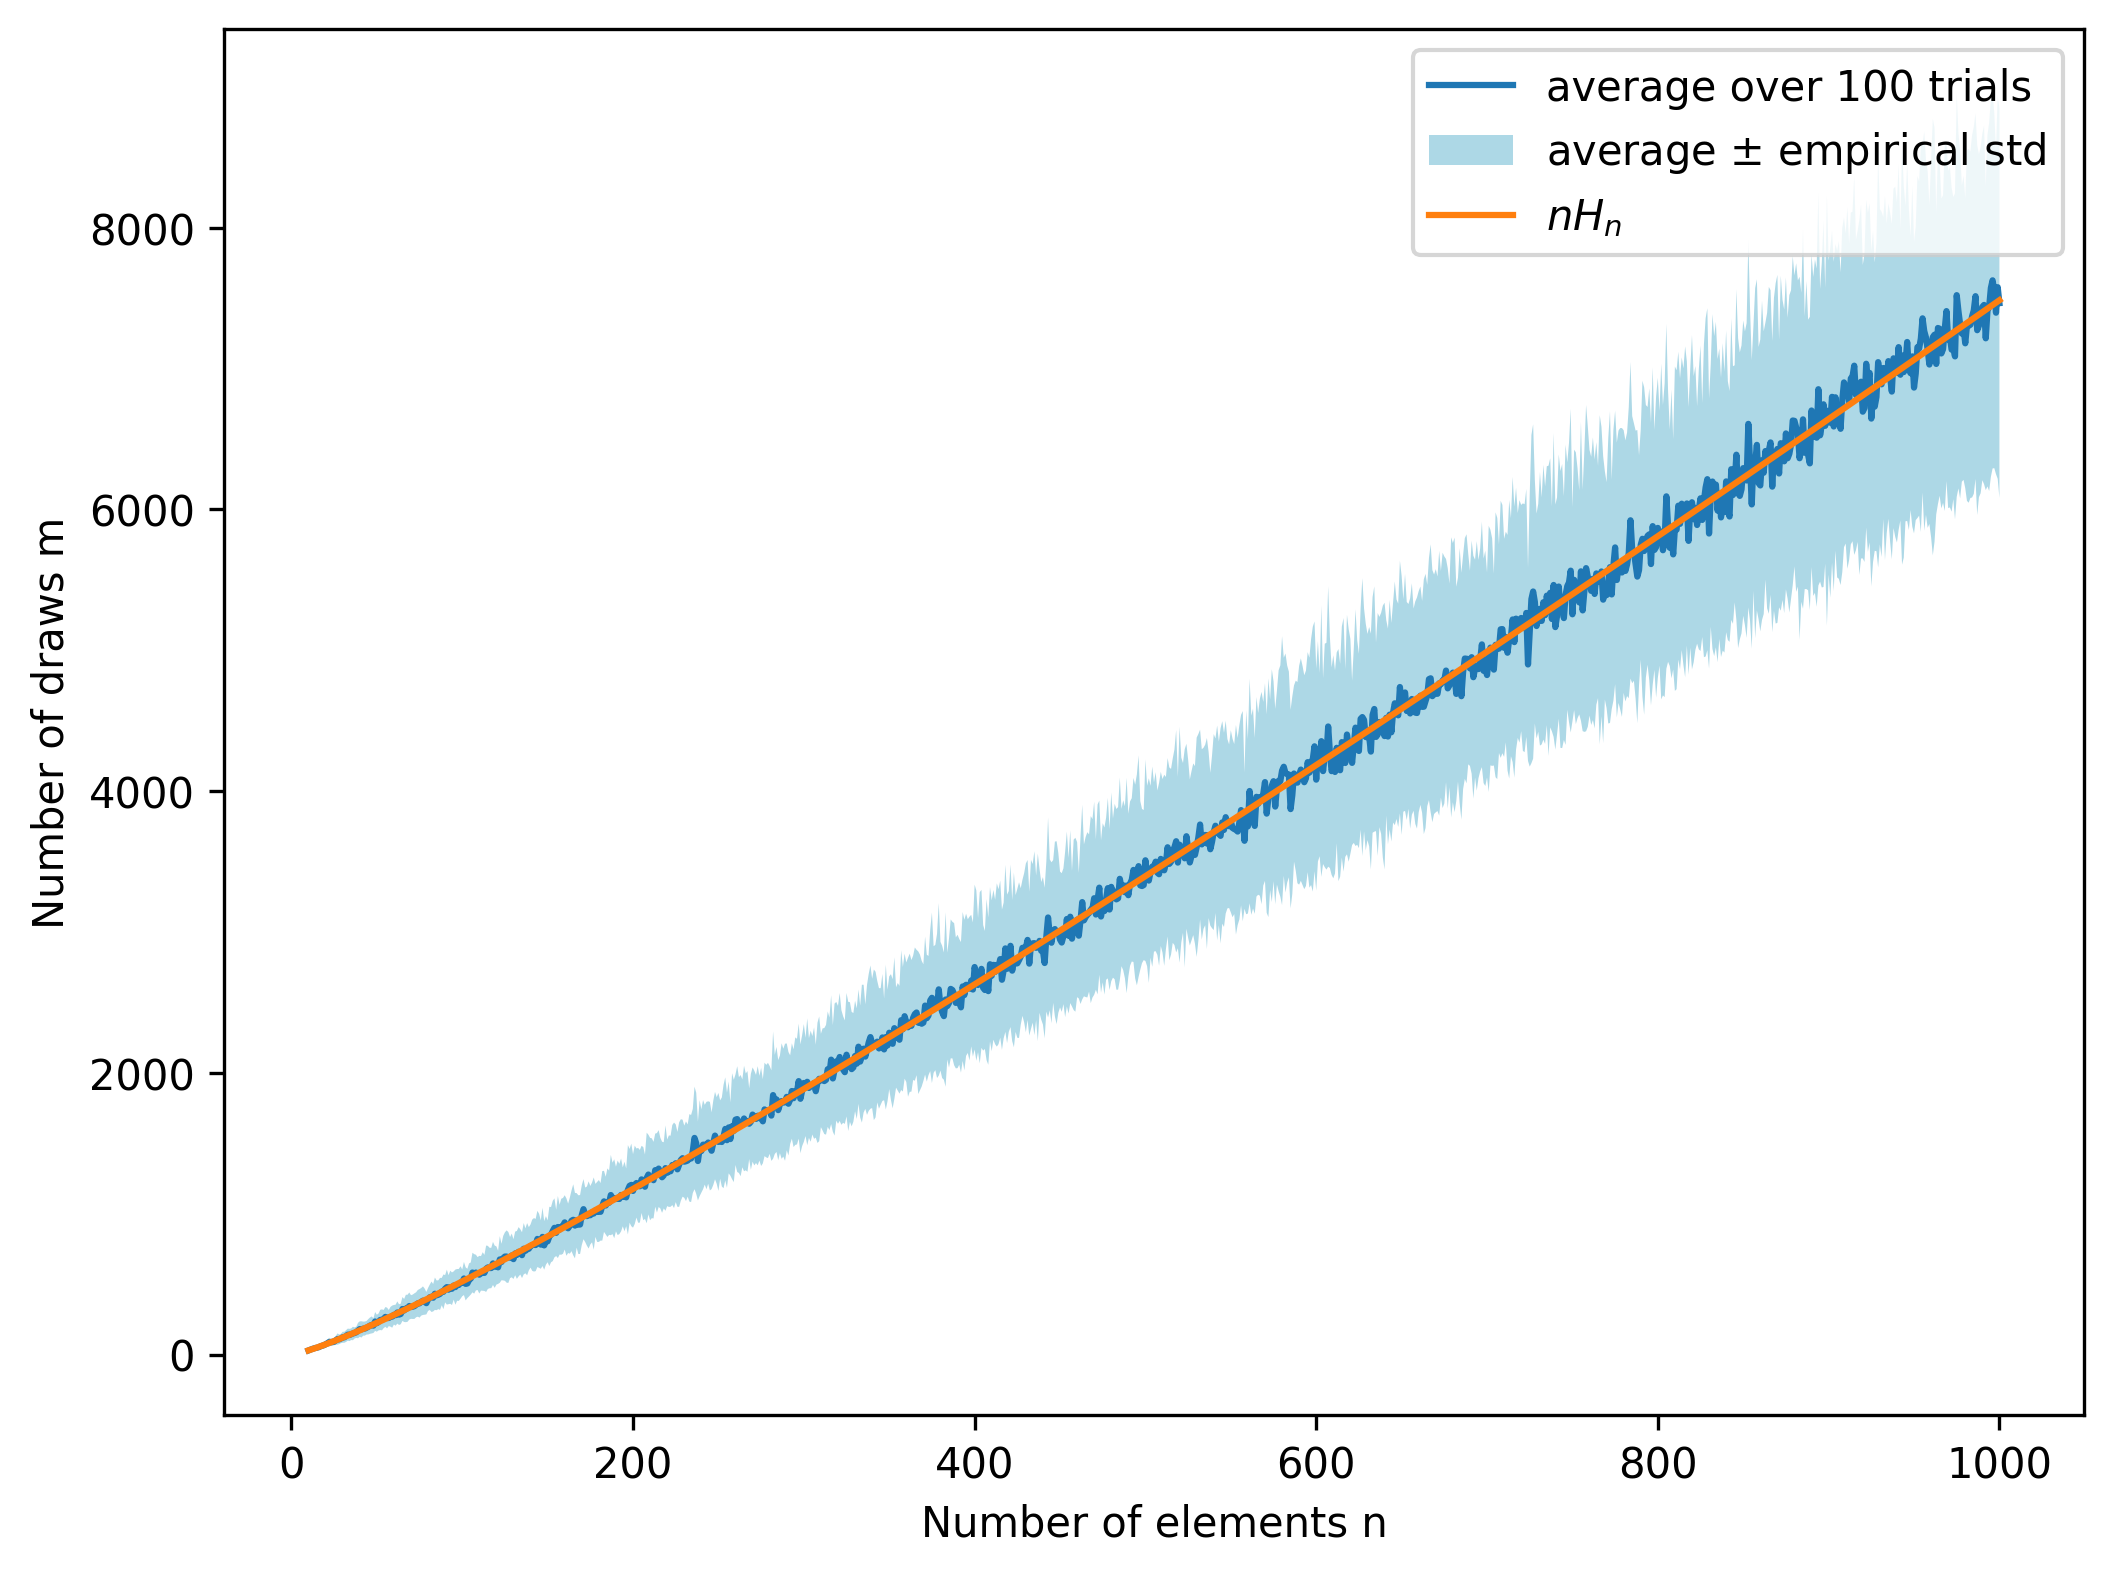
\includegraphics[width=0.9\textwidth]{figures/fig-coverage2.png}
\caption{Average (over 100 trials) of the number of balls thrown until all of the $\nbins$ bins contain at least one ball, as a function of $\nbins$, along with the theoretical value $\nbins H_{\nbins}$ shown in~\cref{theo:coupon:collector:expectation}. The range given by one empirical standard deviation is plotted alongside.}
\end{figure}

Not bad! That does it for the expectation\dots{} but the figure also hints the variance is not too bad, and the number of balls needed to hit all $\nbins$ looks quite concentrated around its expectation. To confirm this (in view of, if we wanted to, applying Chebyshev's inequality), can we also compute the variance?

The amazing thing is that not only we \emph{can}, it's also quite easy.
\begin{theorem}
    \label{theo:coupon:collector:variance}
    The variance of the number $\green{m}(\nbins)$ of bins needed to hit all $\nbins$ bins satisfies
    \[
    \var[\green{m}(\nbins)] \leq \frac{\pi^2}{6}\nbins^2\,.
    \]
\end{theorem}
\begin{proof}
    We start as in the proof of~\cref{theo:coupon:collector:expectation}, writing
    \[
        \green{m}(\nbins) = T_1+\dots+T_{\nbins}
    \]
    The crucial observation is that (suprinsingly?), \emph{the random variables $T_1,\dots,T_{\nbins}$ are independent.} Intuitively, this is because, once you have hit $i-1$ bins, the number of \emph{new} balls you need to cover the remaining $\nbins-(i-1)$ does not depend on how many balls you already threw: it only depends on $\nbins$ and $i$, and ``doesn't care about the past.''\marginnote{This is called the \href{https://en.wikipedia.org/wiki/Geometric_distribution\#General_properties}{memorylessness property} of the geometric distribution, but try to first convince yourself of this without giving it a label.}

    This is great, because computing the variance becomes immediate:
    \[
    \var[\green{m}(\nbins)]=\var[T_1+\dots+T_{\nbins}]
    = \sum_{i=1}^{\nbins} \var[T_i]
    \]
    and we already saw that $T_i \sim \operatorname{Geom}\Paren{p_i}$ with $p_i=\frac{\nbins-i+1}{\nbins}$, ``so'' its variance is \marginnote{Check it yourself: we don't lose much by ignoring the $-p_i$ term.}
    \[
    \var[T_i] = \frac{1-p_i}{p_i^2} \leq \frac{1}{p_i^2}= \frac{\nbins^2}{(\nbins-i+1)^2}
    \]
    and we get
    \[
    \var[\green{m}(\nbins)]
    \leq \nbins^2\cdot\sum_{i=1}^{\nbins} \frac{1}{(\nbins-i+1)^2}
    =\nbins^2\cdot\sum_{j=1}^{\nbins} \frac{1}{j^2}
    \leq \nbins^2\cdot \frac{\pi^2}{6}\,,
    \]
    the last inequality recalling that
    $\sum_{k=1}^{\infty}\frac{1}{k^2} = \frac{\pi^2}{6}$.
\end{proof}
We won't go through too much here, but for instance, by Chebyshev's inequality, this means that
\begin{equation}
    \green{m}(\nbins) = \nbins H_{\nbins} \pm O(\nbins)
\end{equation}
with probability at least $0.99$; combining this with~\cref{fact:harmonic}, similarly,
\begin{equation}
    \green{m}(\nbins) = \nbins \ln \nbins \pm O(\nbins)
\end{equation}
with probability at least $0.99$ (with a different constant in the $O(\cdot)$).

To conclude this part\dots{} how did we do with this variance bound? Well, let us see the empirical simulation again, adding them to the mix:
\begin{figure}[htbp]\centering
    \label{fig:coverage:3}
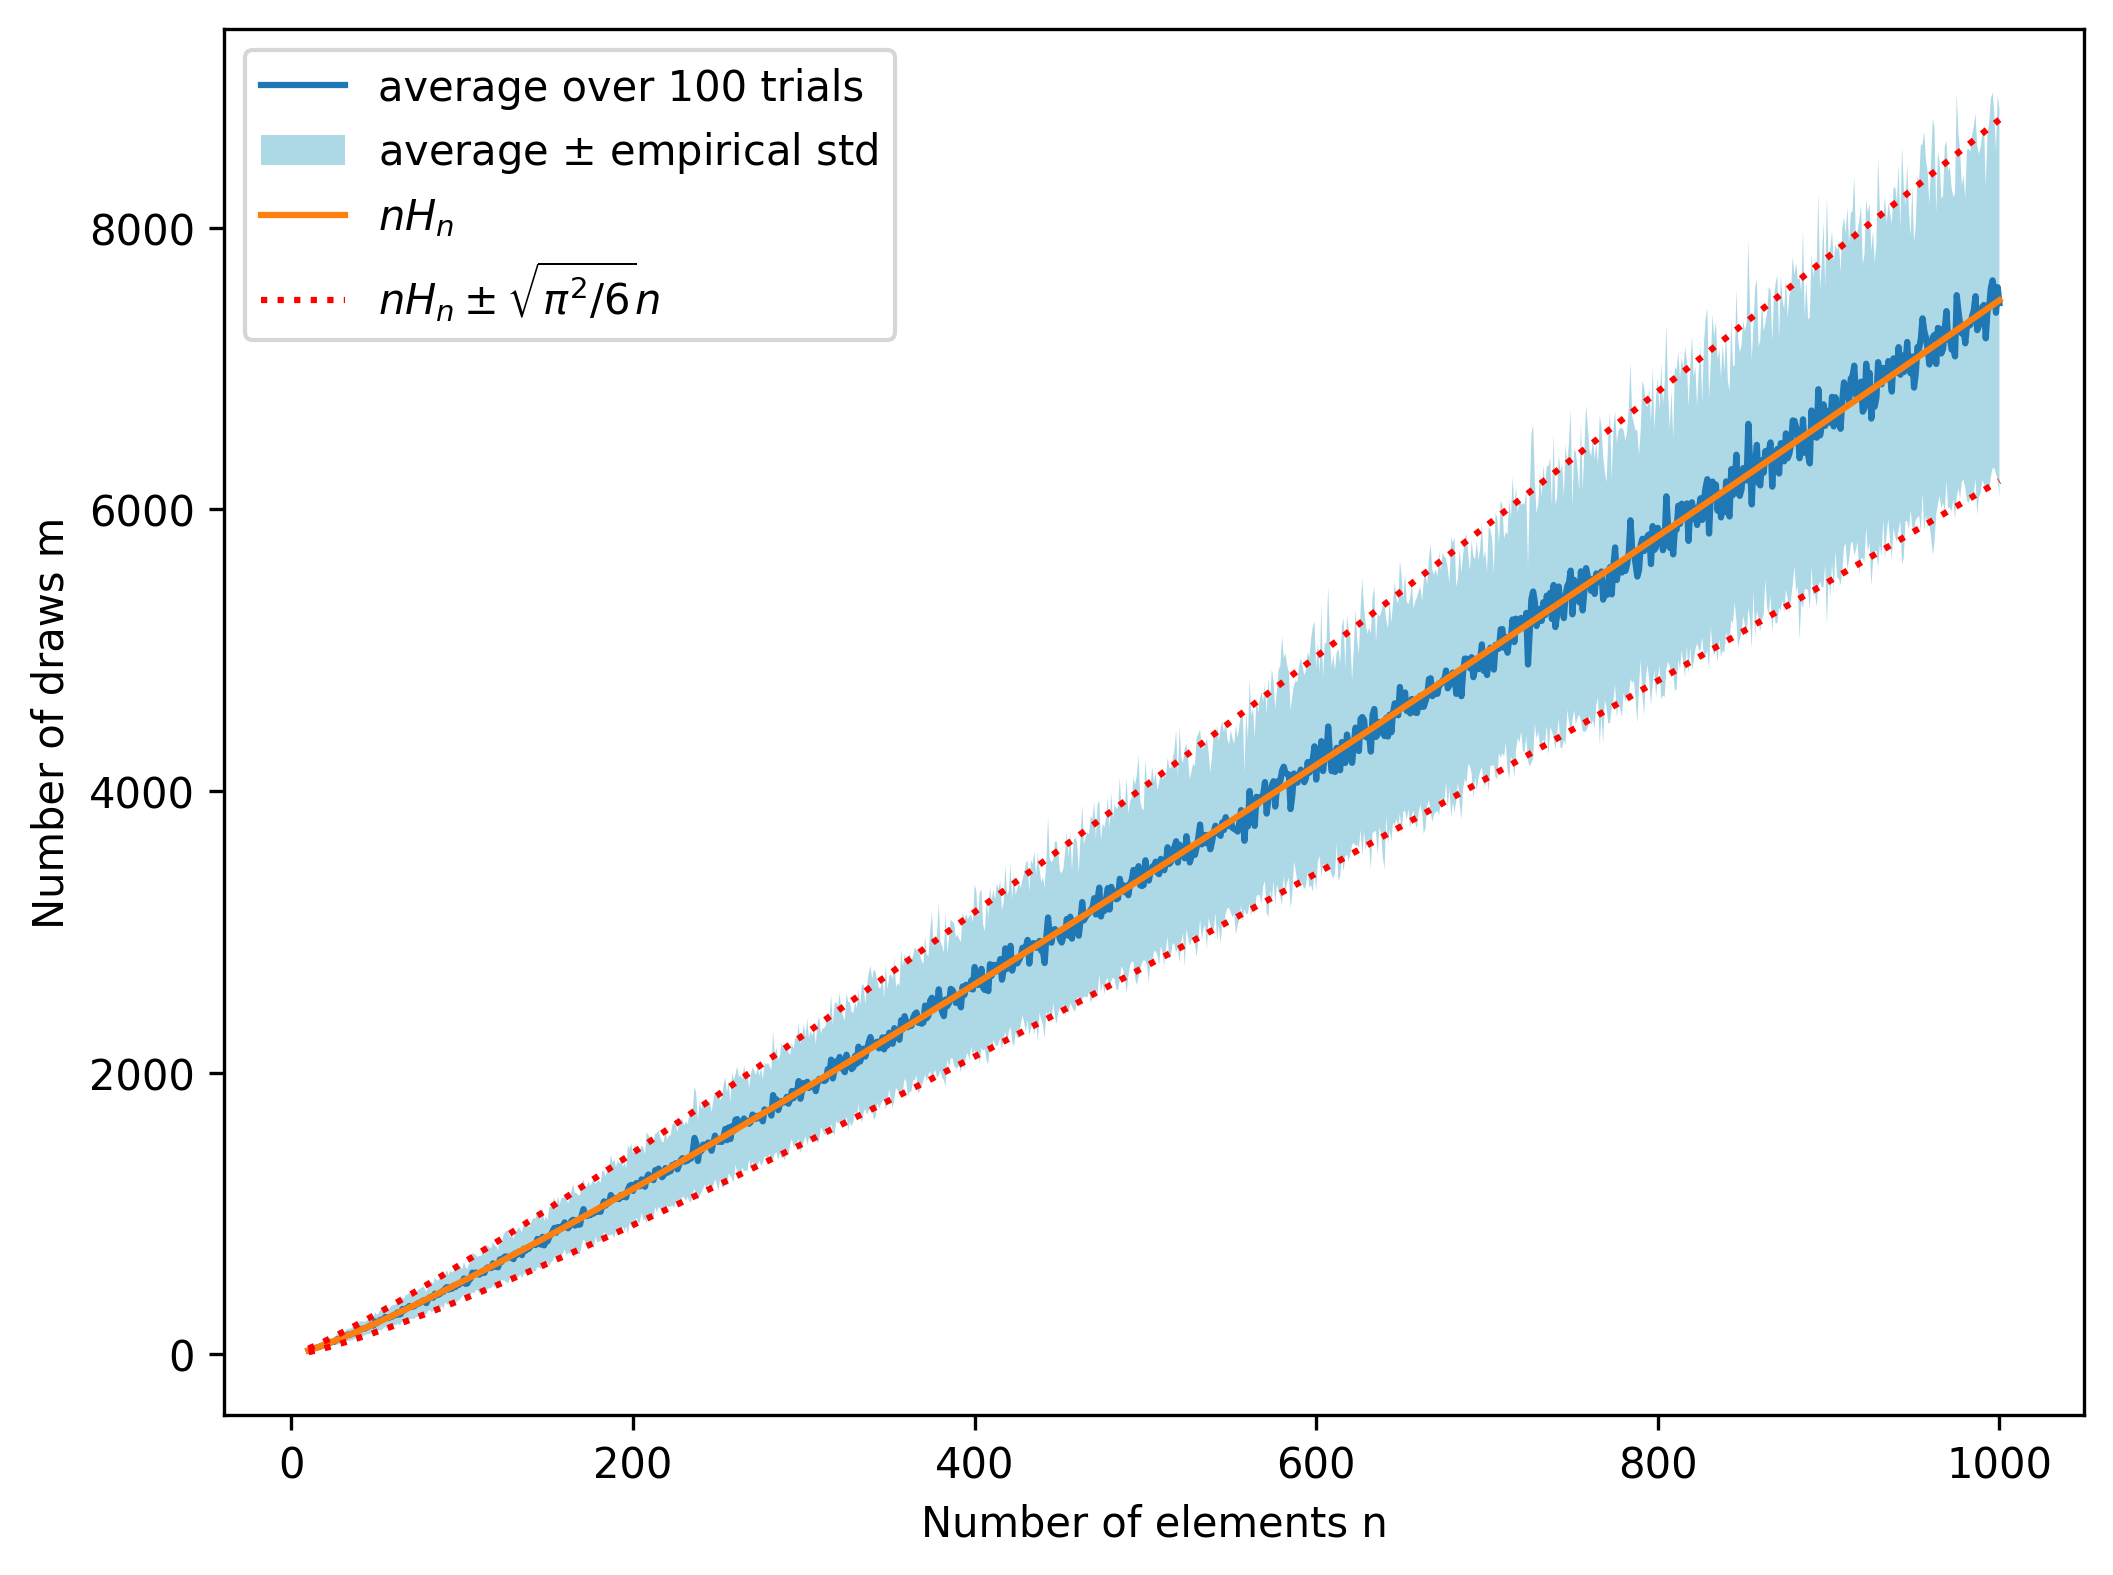
\includegraphics[width=0.9\textwidth]{figures/fig-coverage4.png}
\caption{Average (over 100 trials) of the number of balls thrown until all of the $\nbins$ bins contain at least one ball, as a function of $\nbins$, along with the theoretical value $\nbins H_{\nbins}$ shown in~\cref{theo:coupon:collector:expectation}. The range given by one empirical standard deviation is plotted alongside, as well as the theoretical standard deviation bound obtained.}
\end{figure}

Quite good!

% fun? https://math.stackexchange.com/questions/4051815/intuition-behind-the-coupon-collector-problem-is-there-inclusion-exclusion-prin

\section{Load balancing}
For the last problem considered in this chapter, let us fix $\nballs = \nbins$, and look at how ``balanced'' the bin contents are. In particular, we will be interested in the \emph{maximum load} of the bins:\marginnote{This has applications to, \eg resource allocations, scheduling, etc.}
\begin{framed}
We throw $\nbins$ balls into $\nbins$ bins: what the (expected) number $\orange{L}(\nbins)$ of balls the \emph{fullest} bin will contain?
\end{framed}
Let us denote by $\orange{L}_1,\dots,\orange{L}_{\nbins}$ the number of balls contained in each of the $\nbins$ bins. We have, of course, $\orange{L}_i \leq \nbins$ (number of balls in total) for every $i$. But that's\dots{} quite weak.

It is not hard to see that each bin, separately, follows a Binomial distribution with parameters $\nbins$ and $1/\nbins$\marginnote{Each $\orange{L}_i$ is a $\binomial{\nbins}{1/\nbins}$ random variable: but $\orange{L}_1,\dots,\orange{L}_{\nbins}$ are \emph{not} independent.} and so bin $i$ will have expected load 
\[
\expect{\orange{L}_i} = \nbins\cdot \frac{1}{\nbins} = 1
\]and we also get 
\[
\var[\orange{L}_i] = \nbins\cdot \frac{1}{\nbins}\Paren{1-\frac{1}{\nbins}} \leq 1
\]
This implies, By Chebyshev's inequality, that for each $1\leq i\leq \nbins$, and setting $t \eqdef \sqrt{2\nbins}$,
\[
\probaOf{ \orange{L}_i \geq 1+\sqrt{2\nbins} } \leq \probaOf{ |\orange{L}_i - \expect{\orange{L}_i}| \geq t } \leq \frac{\var[\orange{L}_i]}{t^2} \leq \frac{1}{2\nbins}
\]
and so, by a union bound over the $\nbins$ bins, 
\[
\probaOf{ \max_{1\leq i\leq\nbins}\orange{L}_i \geq 1+\sqrt{2\nbins} } \leq \nbins\cdot \frac{1}{2\nbins} =  \frac{1}{2}
\]
That ``simple'' application of Chebyshev shows the maximum load $\orange{L} = \max_{1\leq i\leq\nbins}$ is $O(\sqrt{\nbins})$ with constant probability. But is it tight? And what does that tell us about $\orange{L}(\nbins)=\expect{\orange{L}}$?\medskip

As in the previous sections, before jumping to conclusions, let's run a simulation.
\begin{lstlisting}
def maxload(n,m):
    loads = np.zeros(n, dtype=int)
    for _ in range(m):
        draw = random.randint(1, n);
        loads[draw-1] += 1
    return np.max(loads)
\end{lstlisting}
\begin{lstlisting}
list_n = np.arange(10, 1001);
experiments_maxload_avg = np.zeros(np.size(list_n));
experiments_maxload_std = np.zeros(np.size(list_n));
for i in range(len(list_n)):
    maxload_trials = [maxload(list_n[i],list_n[i]) for _ in range(100)];
    experiments_maxload_avg[i] = np.mean(maxload_trials);
    experiments_maxload_std[i] = np.std(maxload_trials);
\end{lstlisting}
\begin{figure}[htbp]\centering
    \label{fig:maxload:1}
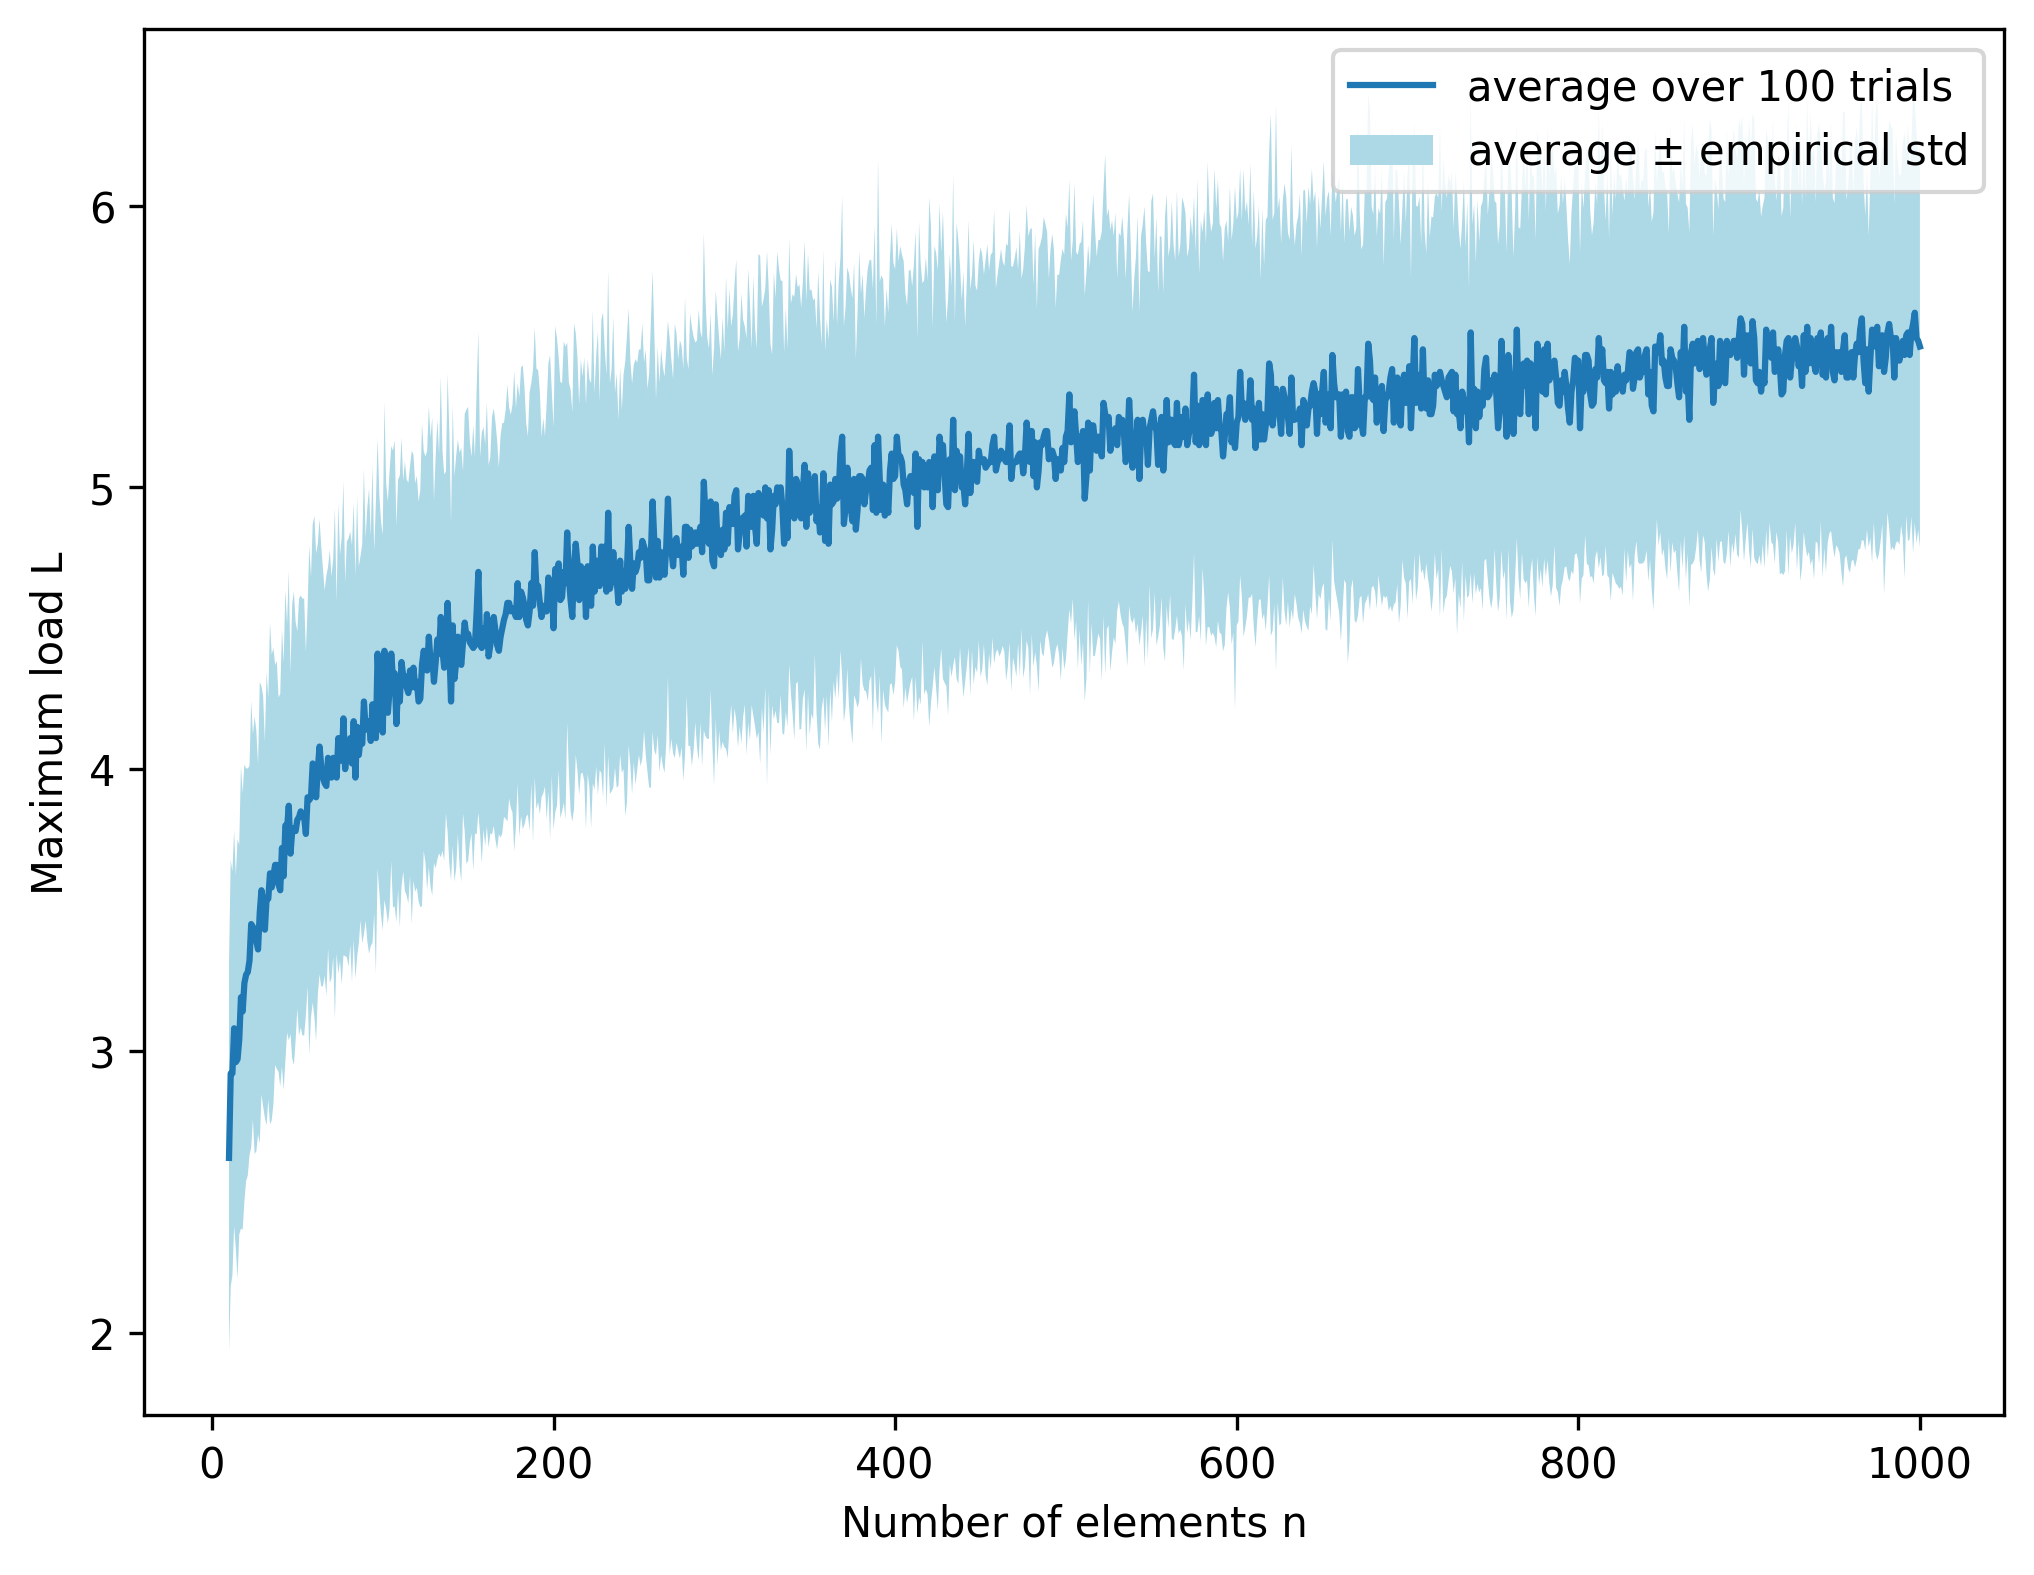
\includegraphics[width=0.9\textwidth]{figures/fig-maxload1.png}
\caption{Average (over 100 trials) of the maximum load when throwing $\nbins$ balls into $\nbins$ bins, as a function of $\nbins$. The range given by one empirical standard deviation is plotted alongside.}
\end{figure}

Looking at the graph (\cref{fig:maxload:1}), we can see how the average maximum load grows with $\nbins$. But what is it, quantitatively? How does $\orange{L}(\nbins)$ behaves?
\begin{itemize}
    \item $\Theta(\log\nbins)$?
    \item $\Theta(\sqrt{\nbins})$?
    \item $\Theta(\nbins)$?
    \item Something else?
\end{itemize}
And \emph{why}?\marginnote{This one will be tough.}\medskip

We will show that, oddly, the answer is ``something else.'' Something quite surprising:
\begin{theorem}
    \label{theo:maxload}
    The expected maximum load $\orange{L}(\nbins)$ when throwing uniformly and independently $\nbins$ balls into $\nbins$ bins grows as
    \[
        \orange{L}(\nbins) = \bigTheta{\frac{\log\nbins}{\log\log\nbins}}\,.
    \]
\end{theorem}
\begin{proof}[Proof of the upper bound of~\cref{theo:maxload}]
Fix any $1\leq i\leq \nbins$, and consider the load in bin $i$. For $0\leq \ell\leq \nbins$, we will give an upper bound on the probability that at least $\ell$ balls fall in this bin: namely, 
\begin{equation}
    \probaOf{\orange{L}_i \geq \ell} 
    \leq \frac{1}{\ell^\ell} 
\end{equation}
To prove this: $\probaOf{\orange{L}_i \geq \ell}$ is the probability that there exists a subset $S\subseteq[\nbins]$ of size at least $\ell$ (a subset of our $\nbins$ balls), and these $|S|$ balls are \emph{exactly} the ones which fell in the $i$-th bin (not a single other): for a fixed $S$, this has probability $\Paren{\frac{1}{\nbins}}^{|S|}\Paren{1-\frac{1}{\nbins}}^{\nbins-|S|}$. We \emph{could} write exactly
\begin{align*}
    \probaOf{\orange{L}_i \geq \ell} 
    &=
    \sum_{\substack{S\subseteq [\nbins]\\ |S| \geq \ell}} \frac{1}{\nbins^{|S|}}\Paren{1-\frac{1}{\nbins}}^{\nbins-|S|} 
    = \sum_{k=\ell}^{\nbins} \sum_{\substack{S\subseteq [\nbins]\\ |S| = k}} \frac{1}{\nbins^{k}}\Paren{1-\frac{1}{\nbins}}^{\nbins-k} \\
    &= \sum_{k=\ell}^{\nbins} \binom{\nbins}{k}\frac{1}{\nbins^{k}}\Paren{1-\frac{1}{\nbins}}^{\nbins-k} %\tag{$\binom{\nbins}{k}$: number of subsets of size $k$}\\
%    &\leq \binom{\nbins}{\ell}\frac{1}{\nbins^{\ell}}\Paren{1-\frac{1}{\nbins}}^{\nbins-\ell}\\
%    &\leq \binom{\nbins}{\ell}\frac{1}{\nbins^{\ell}} 
\end{align*}
the last line recalling that $\binom{\nbins}{k}$ is number of subsets of $[\ns]$ of size $k$, and try to bound that last expression: it is possible, but rather annoying (as binomial coefficients often are), and we do not need to be \emph{that} precise: we just need a good enough upper bound! So we can instead allow ourselves a bit of double-counting: let us simply sum over all subsets $S$ of size \emph{exactly} $\ell$, and focus on the probability that all these $\ell$ balls fall in bin $i$. The other $\ns-\ell$ balls could fall anywhere, including in bin $i$:\footnote{That's the ``we may be double-counting some events'' part.} we don't really care, as long as the upper bound we end up with is not too loose.\marginnote{Exercise: check that $\sum_{k=\ell}^{\nbins} \binom{\nbins}{k}\frac{1}{\nbins^{k}}\Paren{1-\frac{1}{\nbins}}^{\nbins-k} \leq \binom{\nbins}{\ell}\frac{1}{\nbins^{\ell}}$ via a direct computation.}
\begin{align*}
    \probaOf{\orange{L}_i \geq \ell} 
    &\leq
    \sum_{\substack{S\subseteq [\nbins]\\ |S| = \ell}} \probaOf{\text{all }\ell \text{ balls indexed by } S \text{ fall in bin } i} \\
    &=  \sum_{\substack{S\subseteq [\nbins]\\ |S| = \ell}} \left(\frac{1}{\ns}\right)^\ell \\
    &= \binom{\nbins}{\ell}\frac{1}{\nbins^{\ell}} \tag{There are $\binom{\ns}{\ell}$ subsets of size $\ell$}
\end{align*}
From here, we will use this \emph{very} convenient and useful inequality on binomial coefficients:\marginnote{Another life saver.}
\begin{fact}
    \label{fact:binom:coeffs}
    For every $1\leq k\leq n$,
    \[
        \Paren{\frac{n}{k}}^k 
        \leq \binom{n}{k} 
        \leq \Paren{\frac{e n}{k}}^k\,.
    \]
\end{fact}
\noindent This directly leads to the claimed bound
\[
    \probaOf{\orange{L}_i \geq \ell} 
    \leq \Paren{\frac{e \nbins}{\ell}}^{\ell}\frac{1}{\nbins^{\ell}} 
    = \frac{e^\ell}{\ell^\ell}\,.
\]
By a union bound over all $1\leq i\leq \nbins$, we can then conclude that, for every $\ell \geq 1$,
\begin{equation}
    \probaOf{\orange{L} \geq \ell} \leq \sum_{i=1}^{\nbins}\probaOf{\orange{L}_i \geq \ell}
    \leq \frac{\nbins e^\ell}{\ell^\ell}
\end{equation}
This is a very good bound for large $\ell$, but it is quite useless for small $\ell$: for instance, for $\ell=1$, it gives a vacuous bound! Of course, another bound we have is $\probaOf{\orange{L} \geq \ell}  \leq 1$. We will need that, too. Let $\ell(\nbins)$ be the smallest value such that\marginnote{This is the value of $\ell$ starting at which we should switch from using $\probaOf{\orange{L} \geq \ell}  \leq 1$ to using $\probaOf{\orange{L} \geq \ell}  \leq \frac{\nbins e^{\ell}}{\ell^\ell}$, as the latter becomes better.}
\begin{equation}
    \ell(\nbins)^{\ell(\nbins)}e^{-\ell(\ns)} \geq \nbins\,.
\end{equation}
Alright: let us proceed to bounding the expectation of $\orange{L}$. We can write, since $\orange{L}$ is a non-negative integer-valued random variable,\marginnote{Dividing the summation in two parts and using a different bound for both is a standard, handy trick.}
\begin{align}
    L(\nbins) = \expect{\orange{L}} 
    &= \sum_{\ell=1}^\infty \probaOf{\orange{L} \geq \ell} \notag\\
    &= \sum_{\ell=1}^{\ell(\nbins)} \probaOf{\orange{L} \geq \ell} + \sum_{\ell=\ell(\nbins)+1}^\infty \probaOf{\orange{L} \geq \ell} \notag\\
    &\leq \sum_{\ell=1}^{\ell(\nbins)} 1 + \sum_{\ell=\ell(\nbins)+1}^\infty \frac{\nbins e^\ell}{\ell^\ell} \tag{Where the action happens} \notag\\
    &\leq \ell(\nbins) + \sum_{\ell=\ell(\nbins)+1}^\infty \frac{\nbins e^\ell}{\ell(\nbins)^\ell} \notag\\
    &= \ell(\nbins) + \frac{\nbins e^{\ell(\nbins)}}{\ell(\nbins)^{\ell(\nbins)}}\sum_{\ell=\ell(\nbins)+1}^\infty \frac{e^{\ell-\ell(\nbins)}}{\ell(\nbins)^{\ell-\ell(\nbins)}} \notag\\
    &= \ell(\nbins) + \frac{\nbins e^{\ell(\nbins)}}{\ell(\nbins)^{\ell(\nbins)}}\sum_{j=1}^\infty \frac{e^j}{\ell(\nbins)^{j}} \notag\\
    &\leq \ell(\nbins) + \sum_{j=1}^\infty \frac{1}{2^{j}} \tag{as $\frac{\nbins e^{\ell(\nbins)}}{\ell(\nbins)^{\ell(\nbins)}} \leq 1$, and $\ell(\nbins)\geq 2e$} \notag\\
    &= \ell(\nbins) + 1 \label{eq:ub:maxload}
\end{align}
so all that remains to do to conclude is to give an upper bound on $\ell(\nbins)$ itself. This part is not too bad: by definition of $\ell(\nbins)$, we know that
\[
    (\ell(\nbins)-1)^{\ell(\nbins)-1}e^{-(\ell(\nbins)-1))} < \nbins
\]
and taking logarithms, we get
$
(\ell(\nbins)-1)\log (e^{-1}(\ell(\nbins)-1)) < \log \nbins
$. One can ``easily''\marginnote{Exercise: show it.} show that this implies
\[
\ell(\nbins) = \bigTheta{\frac{\log\nbins}{\log\log\nbins}}
\]
which combined with~\eqref{eq:ub:maxload} proves that
$
\boxed{L(\nbins) = \bigO{\frac{\log\nbins}{\log\log\nbins}}}
$.

\paragraph{What about the lower bound?} We will only \emph{sketch} the lower bound in these notes, trying to focus on the key insights. The first insight is that $\orange{L}_1, \dots, \orange{L}_{\nbins}$, which are Binomial r.v.'s with parameters $\nbins$ and $1/\nbins$, are well approximated by a different, ``nicer'' type of of random variable, \emph{Poisson} random variables with parameter $\nbins\cdot 1/\nbins=1$. \marginnote{More generally, 
\[
\boxed{\binomial{n}{\frac{\lambda}{n}} \approx \poisson{\lambda}}
\]
for constant $\lambda>0$. This is very handy!} So we will ``assume'' for convenience\marginnote{This is not an actual proof! But it can be turned into one.} that we can instead consider $\orange{L}'_1, \dots, \orange{L}'_{\nbins} \sim \poisson{1}$. What's more, we will even make the (also not justified! But good for intuition) that these $\orange{L}'_1, \dots, \orange{L}'_{\nbins}$ are independent.

We then can write, since $\expect{\orange{L}} = \sum_{k=1}^\infty \probaOf{\orange{L} \geq k}$, that, for any fixed $\ell\geq 1$ of our choosing,
\begin{align*}
\expect{\orange{L}} &\geq \sum_{k=1}^\ell \probaOf{\orange{L} \geq k} \geq \ell \probaOf{\orange{L} \geq \ell} = 
\ell \probaOf{\exists i,\, \orange{L}_i \geq \ell}
\\
&\approx \ell \probaOf{\exists i,\, \orange{L}'_i \geq \ell}
\geq  \ell \probaOf{\exists i,\, \orange{L}'_i = \ell}
\end{align*}
where the $\approx$ is the first ``sketchy'' Poisson approximation. Using our (unwarranted, sketchy) independence of the $\orange{L}'_i$'s, we can continue by writing\marginnote{If $N\sim\poisson{\lambda}$, then for every non-negative integer $k$
\[
\boxed{\probaOf{N=k} = e^{-\lambda}\frac{\lambda^k}{k!}\,.}
\]}
\begin{align*}
\probaOf{\exists i,\, \orange{L}'_i = \ell}
&= 1-\probaOf{\forall i,\, \orange{L}'_i \neq \ell} \\
&= 1-\Paren{ 1- \frac{e^{-1}}{\ell!} }^{\nbins} \tag{Independence}\\
&\geq 1-e^{-\frac{\nbins}{\ell!}} \tag{using $\ln(1-x)\geq -x$}\\
&\geq 1-e^{-\frac{\nbins}{\ell^\ell}} \tag{using $\ell! \leq \ell^\ell$}\\
\end{align*}
Suitably choosing \[
\ell = \bigTheta{\frac{\log\nbins}{\log\log\nbins}}
\] we get $e^{-\frac{\nbins}{\ell^\ell}} \leq 1/2$, from which $\probaOf{\exists i,\, \orange{L}'_i = \ell} \geq 1/2$. So overall (again, modulo the sketchy bits~--~this is not a full proof), we get
\[
\expect{\orange{L}} \geq \ell \cdot \frac{1}{2} = \bigOmega{\frac{\log\nbins}{\log\log\nbins}}
\]
``showing'' the lower bound.
\end{proof}

\paragraph{Alternative (advanced) proof of the upper bound \advancedstuff} Here is a ``slick'' proof, which seems somewhat magical, but has a couple neat tricks that you will see again or are worth internalizing.\marginnote{Go over it during the tutorials!}

Recall that we want to bound the quantity
\[
\orange{L}(\nbins) = \expect{\max_{1\leq i\leq \nbins} \orange{L}_i}
\]
where the loads $L_1,\dots,L_{\nbins}$ are \emph{not} independent, but all follow a $\operatorname{Binom}(\nbins, 1/\nbins)$ distribution. One can then give an upper bound on $\orange{L}(\nbins)$ as follows.\marginnote{The idea is to replace the $\max$ by a $\sum$ in order to use linearity of expectation~--~but $\max_i \leq \sum_i$ is too lossy, so first we ``exponentiate'' the random variables to mitigate that loss,  as $\max_i \exp \leq \sum_i \exp$ should be ``exponentially less lossy.'' \emph{But} to exponentiate we write $X = \ln \exp X$, which means we now have a $\log$ inside the expectation, and that is not easy to handle: thankfully, $\ln$ is concave, so we can use Jensen's inequality to write $\expect{\ln} \leq \ln\expect{}$. We might also lose something in this step, but that ``Jensen gap'' is typically small for nice, well-concentrated random variables, so\dots{} we can try and hope for the best.}
First, introduce a free parameter $\blue{t}>0$ to be determined later, when we want to optimise the final bound we get.
\begin{align}
    \orange{L}(\nbins) &= \frac{1}{\blue{t}}\cdot \expect{\max_{1\leq i\leq \nbins} \blue{t}\orange{L}_i} \notag\\
    &= \frac{1}{\blue{t}}\cdot \expect{\ln e^{\max_{1\leq i\leq \nbins} \blue{t}\orange{L}_i}} \notag\\
    &\leq \frac{1}{\blue{t}}\cdot \ln\expect{ e^{\max_{1\leq i\leq \nbins} \blue{t}\orange{L}_i}} \tag{Jensen's}\\
    &= \frac{1}{\blue{t}}\cdot \ln\expect{\max_{1\leq i\leq \nbins} e^{\blue{t}\orange{L}_i}} \tag{$\exp{\max_i} = \max_i \exp$}\\
    &\leq \frac{1}{\blue{t}}\cdot \ln\expect{\sum_{1\leq i\leq \nbins} e^{\blue{t}\orange{L}_i}} \tag{$\max_i\leq \sum_i$}\\
    &= \frac{1}{\blue{t}}\cdot \ln \sum_{1\leq i\leq \nbins} \expect{e^{\blue{t}\orange{L}_i}} \tag{Linearity}\\
    &= \frac{1}{\blue{t}}\cdot \ln \nbins \expect{e^{\blue{t}\orange{L}_1}} \label{eq:mgf:maxload}%\\
    %&= \frac{1}{\blue{t}}\Paren{ \ln \nbins + \ln\expect{e^{\blue{t}\orange{L}_1}} }
\end{align}
where the last step used the fact that $L_1,\dots, L_{\nbins}$ all have the same distribution. Now, this quantity $\expect{e^{\blue{t}\orange{L}_1}}$ is called the \emph{moment-generating function} (MGF) of the random variable $\orange{L}_1$, and as a function of $\blue{t}$ it encodes a lot of information about the distribution of $\orange{L}_1$. Thankfully, we do \emph{not} have to compute it: it is standard enough that Wikipedia lists the MGFs for most probability distributions of interest, and in particular for a Binomial random variable $X$ with parameters $n$ and $p$ we have
\begin{equation}
    \expect{e^{tX}} = (1+(e^t-1)p)^n, \qquad t\in\R
\end{equation}
In our case, $p = 1/\nbins$, so we get
\[
    \expect{e^{\blue{t}\orange{L}_1}} 
    = \Paren{1+\frac{e^{\blue{t}}-1}{\nbins}}^{\nbins}
\]
and, using this along with the standard inequality $\ln(1+x) \leq x$ ($x> -1$) in~\eqref{eq:mgf:maxload},\marginnote{This one is a life saver.}
\begin{align}
    \orange{L}(\nbins) 
    &\leq \frac{1}{\blue{t}}\Paren{ \ln \nbins + \ln\expect{e^{\blue{t}\orange{L}_1}} } \notag\\
    &\leq \frac{1}{\blue{t}}\Paren{ \ln \nbins + \nbins\ln\Paren{1+\frac{e^{\blue{t}}-1}{\nbins}} } \notag\\
    &\leq \frac{1}{\blue{t}}\Paren{ \ln \nbins + e^{\blue{t}}-1 } \label{eq:mgf:maxload:freeparam}
\end{align}
We're almost there! We still have our free parameter $\blue{t}>0$, and we get to choose it however we want in order to get the best upper bound possible (we get a valid upper bound no matter which $\blue{t}$ we pick). One option to do so would be to differentiate the RHS of~\eqref{eq:mgf:maxload:freeparam} to find the minimum: this is unfortunately quite unwieldy. A simpler (and most of the time ``good enough''\marginnote{If one does not care too much about the exact constant factors or lower-order terms.} is to observe that
\begin{equation}
\max(a,b) \leq a+b \leq 2\max(a,b), \qquad a,b\geq 0
\end{equation}
and so \emph{minimising a sum of two terms is roughly the same as minimising the maximum.} Here we have two terms: $\ln \nbins$ and $e^{\blue{t}}-1$: one way to make sure the maximum is not too bad is to ``balance it out'', and choose $\blue{t}$ so that the two terms are equal.\marginnote{Useful trick: avoids calculus.} In our case, this means choosing
\begin{equation}
\blue{t} \eqdef \ln\Paren{1+\ln \nbins} = \ln\ln(e\nbins)
\end{equation}
and plugging this choice of $\blue{t}$ in~\eqref{eq:mgf:maxload:freeparam} gives
\begin{equation}
    \label{eq:mgf:maxload:end}
    \orange{L}(\nbins)
    \leq \frac{2\ln \nbins}{\ln\ln(e\nbins)}\,.
\end{equation}
We're done!


\section{Load balancing: the power of two choices}
To conclude, let us mention an even more counter-intuitive result: imagine that instead of throwing $\nbins$ balls uniformly into $\nbins$ bins, each ball instead selects \emph{two} bins uniformly at random, and falls into the \emph{least} full of the two (breaking ties arbitrarily).\marginnote{This looks strange, but has applications to hashing, task allocation, network broadcasting\dots} What becomes the expected maximum load?

As usual, let us first try to get a sense of what is going on via a simulation:
\begin{lstlisting}
def maxload2choices(n,m):
    loads = np.zeros(n, dtype=int)
    for _ in range(m):
        draw1 = random.randint(1, n);
        draw2 = random.randint(1, n);
        if loads[draw2-1] > loads[draw1-1]:
            loads[draw1-1] += 1
        else:
            loads[draw2-1] += 1
    return np.max(loads)
\end{lstlisting}
\begin{lstlisting}
list_n = np.arange(10, 1001);
experiments_maxload2choices_avg = np.zeros(np.size(list_n));
experiments_maxload2choices_std = np.zeros(np.size(list_n));
for i in range(len(list_n)):
    maxload2choices_trials = [maxload2choices(list_n[i],list_n[i]) for _ in range(100)];
    experiments_maxload2choices_avg[i] = np.mean(maxload2choices_trials);
    experiments_maxload2choices_std[i] = np.std(maxload2choices_trials);
\end{lstlisting}
\begin{figure}[htbp]\centering
    \label{fig:maxload:2}
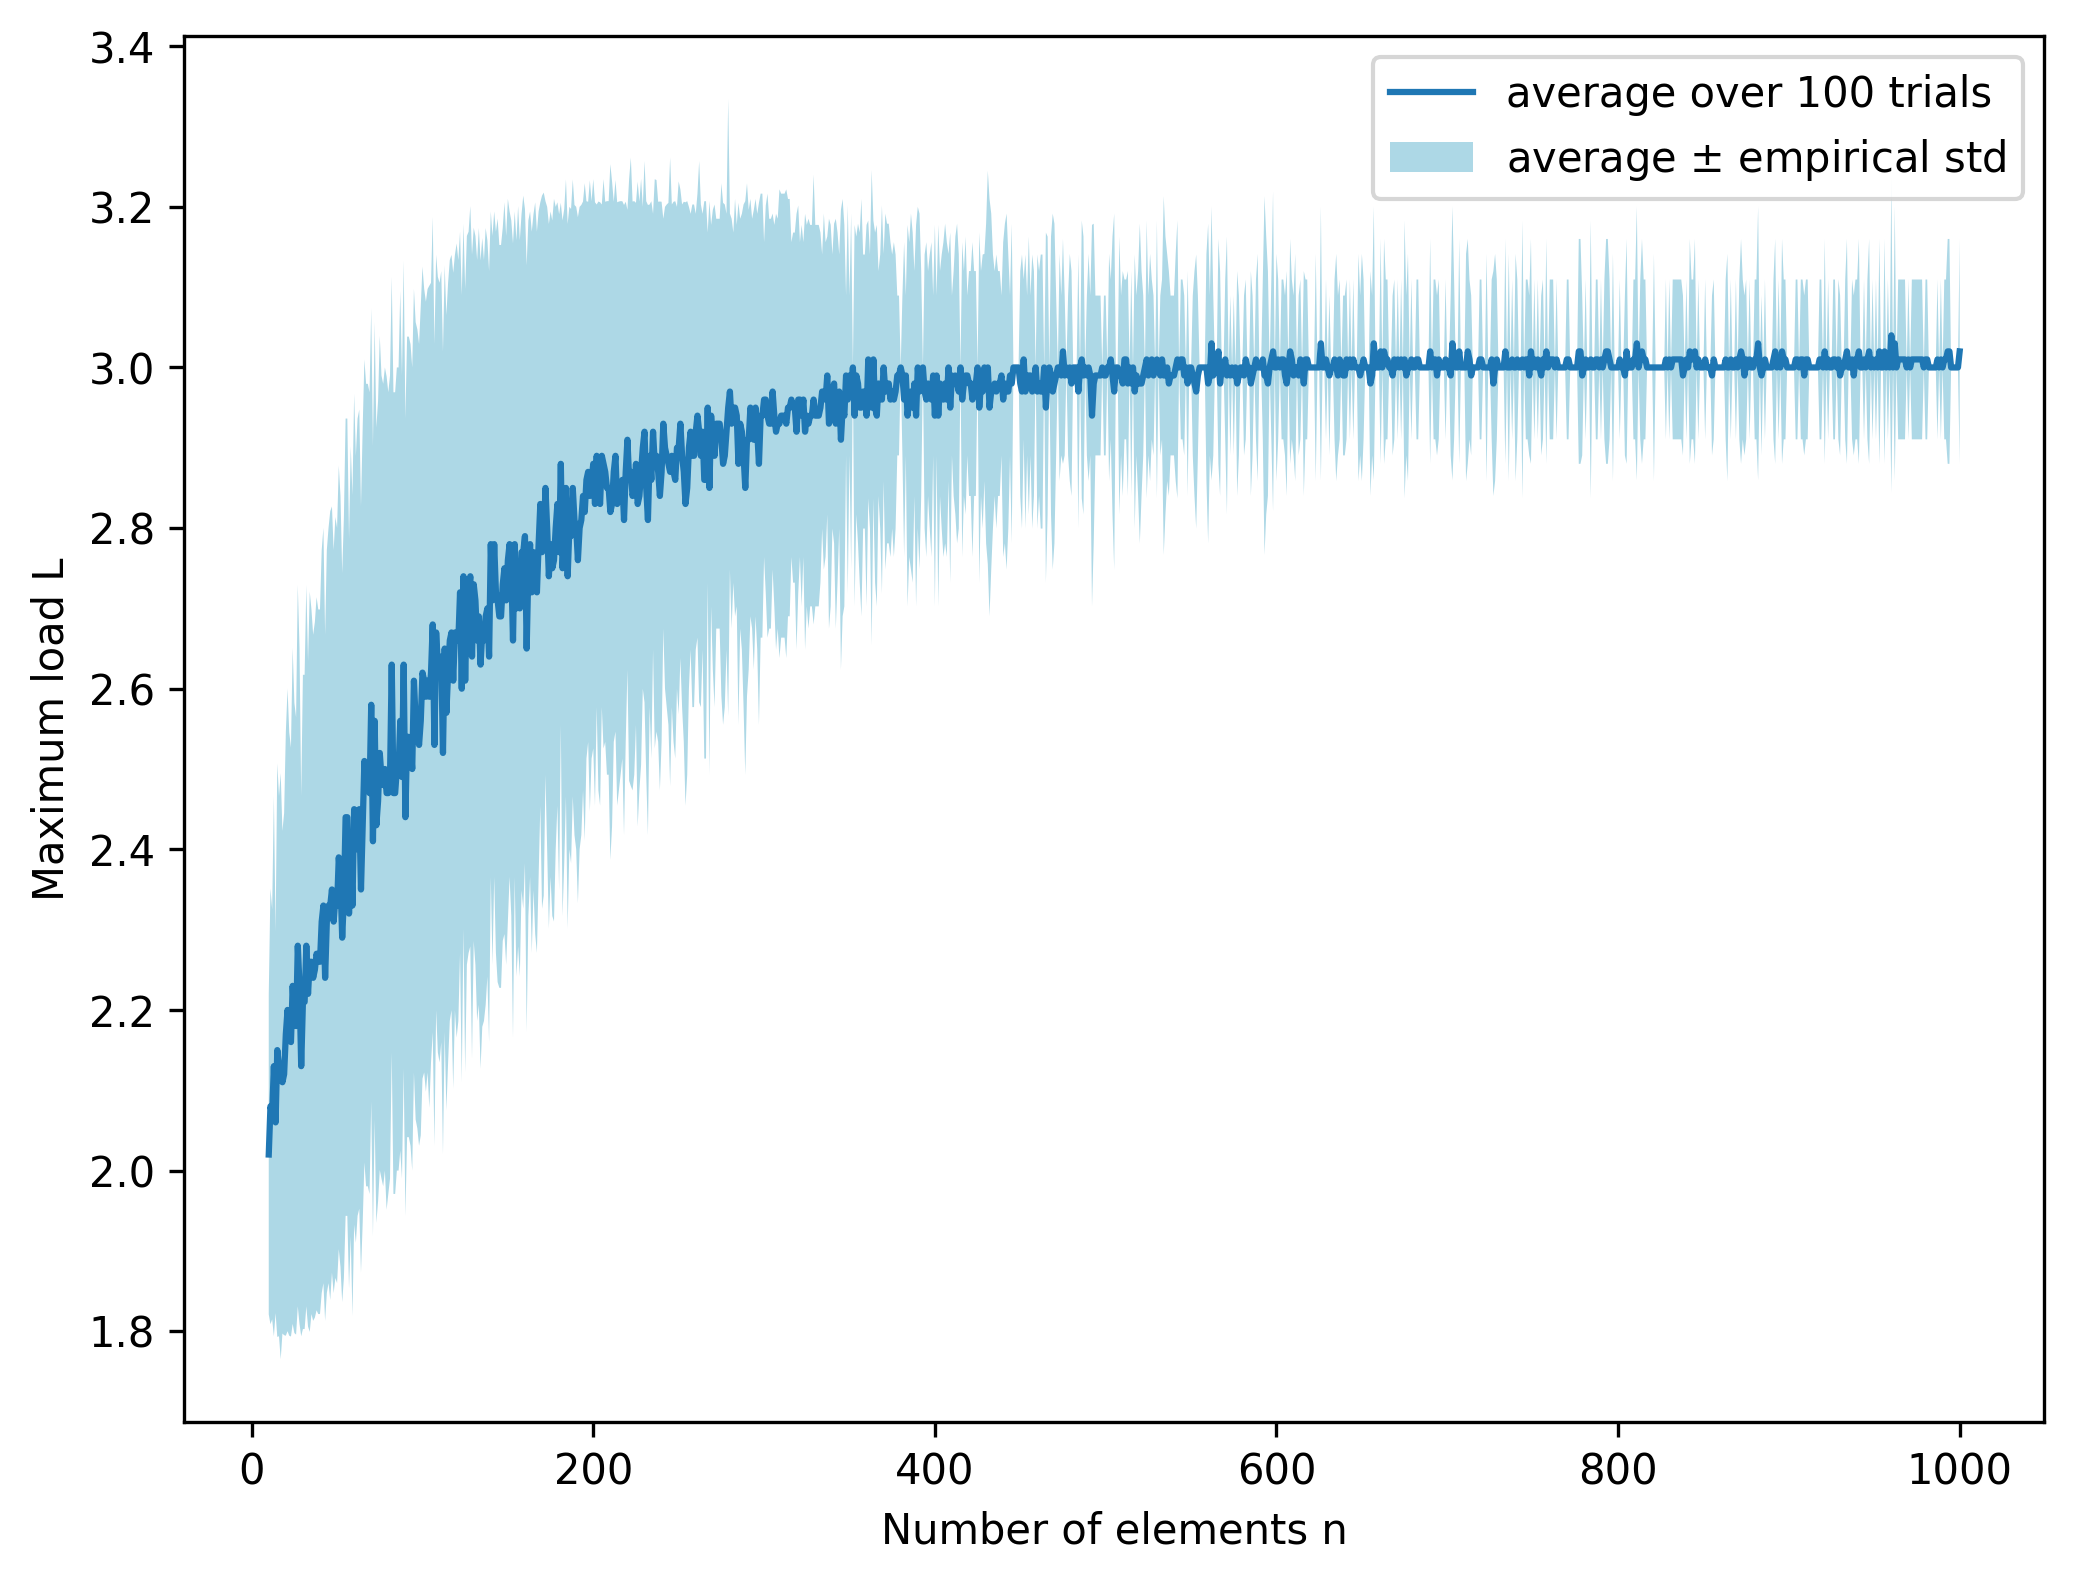
\includegraphics[width=0.9\textwidth]{figures/fig-maxload2choices.png}
\caption{Average (over 100 trials) of the maximum load when throwing $\nbins$ balls into $\nbins$ bins, using the ``best of two bins'' strategy for each bin, as a function of $\nbins$. The range given by one empirical standard deviation is plotted alongside.}
\end{figure}

Looking at the graph (\cref{fig:maxload:2}), we can see that with this ``best of two choices'' the maximum load grows much slower (as a function of $\nbins$) than in the previous setting (\cref{fig:maxload:1}). But how much slower? %How does $\orange{\hat{L}}(\nbins)$ behaves?
\begin{itemize}
    \item $\Theta(\sqrt{\log\nbins})$?
    \item $\bigTheta{\frac{\log\nbins}{(\log\log\nbins)^2}}$?
    \item $\Theta(\log\log\nbins)$?
    \item Something else?
\end{itemize}
\marginnote{\TODO{} in class: Visualization of the maximum load as $\nballs$ increases, i.e., as more balls are thrown (same with power of two choices).}

\noindent Amazingly, this simple ``power of two choices'' brings the expected maximum load from $\bigTheta{\frac{\log\nbins}{\log\log\nbins}}$ to something \emph{exponentially smaller}:
\begin{theorem}
    \label{theo:maxload:twochoices}
    The expected maximum load $\orange{\hat{L}}(\nbins)$ when throwing independently $\nbins$ balls into $\nbins$ bins using the ``best of two choices'' strategy above grows as
    \[
        \orange{\hat{L}}(\nbins) = \log\log\nbins + O(1)\,.
    \]
\end{theorem}
\noindent(We will not prove this theorem in the lecture.)

\chapter{Lecture 4: Derandomisation}
Sometimes, having a randomised algorithm is wonderful, but what we really need is a \emph{deterministic} version that achieves the same guarantees, but without the drawback of randomness: that is, we want the output to \emph{always} be good (unlike Monte Carlo-type algorithms), and the running time to \emph{always} be bounded (unlike Las Vegas-type algorithms). That is, we would like to be able, given any randomised algorithm $\Algo$, to ``derandomise'' it into an equally-good (or not much worse) deterministic version $\Algo'$. \emph{Can we achieve that?}

Unsurprisingly, the answer is a resounding ``we don't know.''\marginnote{This is actually very much tied to one of the central questions in computational complexity, the $\textsf{P}$ vs. $\textsf{BPP}$ question.} However, we do have some (limited) techniques to do so, in particular cases. Here, we will see two of them: the \emph{small random seed approach} and the \emph{method of conditional expectations}.

To illustrate this, we will consider as running example the ``maximum cut'' question:
\begin{framed}
\noindent \textsc{Max-Cut}: Given an (undirected) graph $G=(\red{V},\orange{E})$ on $\red{n}$ vertices and $\orange{m}$ edges, output a cut $(A,B)$ (partition of $\red{V}$) \emph{maximising} the number $c(A,B)$ of edges between $A$ and $B$.
\end{framed}
Of course, we would like an efficient algorithm for that. As a baseline, one could try to ``just'' find a good algorithm to solve the problem. Unfortunately, this is very unlikely to pan out:
\begin{fact}
    $\textsc{Max-Cut}$ is NP-Hard.
\end{fact}
This is annoying, as this strongly hints we should give up on trying to find an efficient algorithm (deterministic, but, also, randomised -- this is most likely very hard too) for $\textsc{Max-Cut}$. An \emph{exact} algorithm, at least: but maybe we can get a good \emph{approximation} algorithm?\footnote{Recall that an $\alpha$-approximation algorithm is an algorithm whose output's value is within a factor $\alpha > 0$ of the optimal solution's value.}

Here is an obvious randomised algorithm: \emph{choose a cut $(A,B)$ uniformly at random.} Or, with more words and in pseudocode:
\begin{algorithm}[H]
\begin{algorithmic}[1]
        \State $(A,B) \gets (\emptyset,\emptyset)$
        \ForAll{$v\in \red{V}$}
            \State $X_v \gets \bernoulli{1/2}$ \Comment{Independent of previous choices} \label{line:random:maxcut:cointoss}
            \If{$X_v = 1$}
            add $v$ to $A$
            \Else\ 
            add $v$ to $B$
            \EndIf
        \EndFor
        \State \Return $(A,B)$
    \end{algorithmic}
    \caption{Randomised algorithm for $\textsc{Max-Cut}$.}
    \label{algo:random:maxcut}
\end{algorithm}
\emph{Is it any good?} Maybe surprisingly, not too bad: in expectation, what it returns is a cut with at least \emph{half} as many edges as the best possible:
\begin{theorem}
    \label{theo:expected:maxcut}
    For every $G=(V,E)$, the output $(A,B)$ of ~\cref{algo:random:maxcut} satisfies 
    \[
    \bEE{c(A,B)} \geq \frac{1}{2}\orange{m} \geq \frac{1}{2}\operatorname{OPT}(G)\,.
    \]
    Moreover, the algorithm runs in time $\bigO{\red{n}}$.
\end{theorem}
\begin{proof}
    The proof is immediate by linearity of expectation. Fix any edge $e\in \orange{E}$ and let $X_e$ denote the indicator random variable ``$e$ is a cut edge'' (that is, one end is in $A$, the other in $B$). It is easy to check that $\bEE{X_e}=1/2$ (both endpoints are in $A$ with probability $1/2\cdot 1/2=1/4$, same for both endpoints in $B$, so an edge crosses with probability $1/2$).

Rewriting $c(A,B)=\sum_{e\in E} X_e$, by linearity of expectation, we get
\[
\bEE{c(A,B)} = \bEE{\sum_{e\in \orange{E}} X_e}= \sum_{e\in \orange{E}}\bEE{X_e} =  \sum_{e\in \orange{E}}\frac{1}{2} = \frac{\orange{m}}{2}
\]
and the last part of the statement follows from observing that the best possible cut cannot have more than $\orange{m}$ edges.
\end{proof}

Can we convert~\cref{algo:random:maxcut} into a \emph{deterministic} (and still efficient) algorithm?

%%%%%%%%%%%%%%%%%%%%%%%%%%%%%%%%%%%%%%%%%%%%%%%%%%%%
\section{Method 1: derandomizing the random seed}
Let us get back to the view of a randomized algorithm from the first lecture, as an ``algorithm $\Algo$ taking an input $x$ and a string of uniformly random bits $\green{r}\in\{0,1\}^\ast$.'' Imagine (1)~$\Algo$ has a positive probability of returning a good solution; (2)~we have a worst-case bound $\green{R}$ on the \emph{randomness complexity} of our algorithm, \ie on the maximum number of random bits it would every need on any input $x$; and (3)~that, given a solution $y$ to the task, that we can \emph{verify} efficiently whether $y$ is a good solution~--~say, by running another algorithm $\orange{V}$ on $(x, y)$.

Then the claim is that the following algorithm is a deterministic algorithm that finds a good solution:
\begin{algorithm}[H]
\begin{algorithmic}[1]
        \Require Input $x$
        \ForAll{$\green{r}\in\{0,1\}^{\green{R}}$}
            \State $y \gets \Algo(x; \green{r})$ \Comment{Run $\Algo$ on $x$ with randomness $\green{r}$}
            \If{$V(x,y) = 1$} \Comment{Verify if $y$ is a good solution}
              \State\Return $y$ \Comment{If so, we are done}
            \EndIf
        \EndFor
    \end{algorithmic}
    \caption{Derandomization approach (by brute-forcing over the random seed)}
    \label{algo:random:derandom:1}
\end{algorithm}
The fact that~\cref{algo:random:derandom:1} always returns a good solution, under our assumptions (1), (2), and (3), is immediate: there exists \emph{some} choice of the randomness $\green{r}$\marginnote{Importantly, this ``good random seed'' $\green{r}$ may not be the same for all $x$.} for which $\Algo$ returns a good solution on input $x$; once we try this particular $\green{r}$ in the loop, then we get a good solution $y$, and the verifier $\orange{V}$ successfully detects it. 

There is, of course, a catch:
\begin{fact}
    \label{fact:derandomization:smallseed}
    \cref{algo:random:derandom:1} runs in time $2^{\green{R}}\Paren{T_{\Algo}+T_{\orange{V}}}$, where $T_{\Algo},T_{\orange{V}}$ are the running times of the algorithm $\Algo$ and verifier $\orange{V}$.
\end{fact}
In particular, given that $\green{R}$ could be quite large (the only \emph{a priori} bound we have is $\green{R} \leq T_{\Algo}$),\marginnote{Can you see why?} this could be really bad \emph{even if $\Algo$ and $\orange{V}$ are efficient}: exponential in the input size, or even worse.

\paragraph{So what to do?} One hope we may have is to get a much better bound on $\green{R}$ for some specific algorithms, or even to slightly modify these algorithms to make sure $\green{R}$ is small. For instance, if we can design a randomised algorithm which only needs say $\green{R} \leq 2\log n$ bits of randomness on inputs of size $n$, then we get $2^{\green{R}} = n^{2}$: that's polynomial!

Looking back at~\cref{algo:random:maxcut}, it \emph{seems} like we are using an awful number of random bits: one for each vertex $v\in \orange{V}$, so $\green{R} = \red{n}$ in total. That is definitely not great. And yet, do we actually \emph{need} this many independent random bits? Could we do with a much smaller number and use something like hash functions?\marginnote{Hash functions are essentially magic: when you know how to use them, they are incredible. When you don't, you end up with a third arm growing out of your ear.}

The only part of the proof of~\cref{theo:expected:maxcut} where we used the randomness was to argue that each edge $e=(u,v)$ is a cut-edge with probability $1/2$. This argument requires independence of the two random bits involved: the random bit $B_u$ for $u$, and the random bit $B_v$ for vertex $v$. That is all: 
\begin{framed}
\noindent\emph{As long as $B_u$ and $B_v$ are independent for each of the $\binom{\red{n}}{2}$ pairs of distinct vertices $(u,v)$, the proof goes through!}
\end{framed}
That is called \emph{pairwise independence}, and this is a \emph{much} weaker requirement than (full) independence. In particular, we can use good hash functions to get pairwise independence very cheaply~--~to see how, let us introduce a key definition:\marginnote{Importantly, here $x,x',y,y'$ are not random! We pick a hash function $\green{h}$ at random and see where it sends the inputs. So $\green{h}$ is a \emph{randomly picked hash function} (among the $\abs{\green{\mathcal{H}}}$ choices), not a ``random function'': once $\green{h}$ is picked, there is nothing random anymore.}
\begin{definition}
    \label{def:universal:pairwise:hash}
    A family of functions $\green{\mathcal{H}} \subseteq \{h\colon \cX \to \cY\}$ is a \emph{family of pairwise independent hash functions},  or a \emph{strongly universal hash family}, if, for every $x,x'\in \cX$ with $x\neq x'$ and every $y,y'\in\cY$,
    \[
        \probaDistrOf{\green{h}\sim \green{\mathcal{H}}}{ \green{h}(x) = y, \green{h}(x') = y' } = \frac{1}{\abs{\cY}^2}
    \]
    where the probability is over the uniformly random choice of~$\green{h}\in\green{\mathcal{H}}$.
\end{definition}
Why does that help? Take the example of $\cX=[\red{n}]$ and $\cY=\{0,1\}$ in the definition above. Picking a hash function $\green{h}\in\green{\mathcal{H}}$ uniformly at random only takes $\log\abs{\green{\mathcal{H}}}$ truly independent random bits. But with these $\log\abs{\green{\mathcal{H}}}$ random bits, we obtain $|\cX|=\red{n}$ random bits
\[
    \green{h}(1), \green{h}(2), \dots, \green{h}(\red{n}) \in \{0,1\}
\]
which are \emph{not} fully independent, but such that \emph{any two of them behaves exactly like a pair of uniformly random bits.} This is exactly what we need! The only missing part is: \emph{do there exist ``small''\marginnote{Small enough, because we want to use as few ``true'' random bits as possible, and that will cost us $\log\abs{\green{\mathcal{H}}}$ of them.} families of pairwise independent hash functions $\green{\mathcal{H}} \subseteq \{h\colon [\red{n}] \to \{0,1\}\}$?} 

\begin{fact}
    \label{fact:pairwise:hash:functions}
    There exists an explicit\footnote{Easy to construct and use. We will prove it in the tutorial!} family of pairwise independent hash functions $\green{\mathcal{H}} \subseteq \{h\colon [\red{n}] \to \{0,1\}\}$ with $\abs{\green{\mathcal{H}}} = 2^{\clg{\log(\red{n}+1)}}$.
\end{fact}

This is great news! Now we can modify~\cref{algo:random:maxcut} to first pick $\green{h}$ uniformly at random from this specific $\green{\mathcal{H}}$ (this only requires $\green{R} \leq \clg{\log(\red{n}+1)}$ bits of randomness), and then use $X_v \gets \green{h}(v)$ as random coin toss for vertex $v$ in~\cref{line:random:maxcut:cointoss}. 

\begin{algorithm}[H]
\begin{algorithmic}[1]
        \State $(A,B) \gets (\emptyset,\emptyset)$
        \State Draw $\green{h}\colon \red{V} \to \{0,1\}$ uniformly at random from the $\green{\mathcal{H}}$ promised by~\cref{fact:pairwise:hash:functions}, using $\green{R}=\clg{\log(\red{n}+1)}$ random bits
        \ForAll{$v\in \red{V}$}
            \State $X_v \gets \green{h}(v)$ \Comment{Pairwise independence}
            \If{$X_v = 1$}
            add $v$ to $A$
            \Else\ 
            add $v$ to $B$
            \EndIf
        \EndFor
        \State \Return $(A,B)$
    \end{algorithmic}
    \caption{(Modified) Randomised algorithm for $\textsc{Max-Cut}$ to use a small random seed.}
    \label{algo:random:maxcut:smallseed}
\end{algorithm}

By pairwise independence, the proof of correctness of this (modified)~\cref{algo:random:maxcut} goes through exactly as in~\cref{theo:expected:maxcut}, but now we use much fewer random bits\dots So, when derandomising the algorithm \emph{via}~\cref{algo:random:derandom:1}, we only pay a factor
\[
    2^{\green{R}} = 2^{\clg{\log(\red{n}+1)}} \leq 2(\red{n}+1) = O(\red{n})
\]
What about the rest? Well, we saw already that $T_{\Algo}=O(\red{n})$. As for the time $T_{\orange{V}}$ it takes to verify a cut $(A,B)$ has size at least $\orange{m}/2$, this is $T_{\orange{V}} = O(\orange{m}+\red{n})$, and so by~\cref{fact:derandomization:smallseed} our ``derandomised algorithm'' has running time at most
\[
    2^{\green{R}}\Paren{T_{\Algo}+T_{\orange{V}}} = \bigO{\red{n}(\orange{m}+\red{n})}\,.
\]
Not bad. But we are missing a small part: one of the assumptions required to derandomise using~\cref{algo:random:derandom:1} was ``(1)~$\Algo$ has a positive probability of returning a good solution.'' We never checked this: all we know is that our randomised algorithm, \cref{algo:random:maxcut:smallseed}, returns a solution that is good (\ie with value at least $\frac{1}{2}\orange{m}$) \emph{in expectation}. Does that mean it has a \emph{positive probability} of returning a good solution?

\noindent Thankfully, yes: it can be arbitrarily small, but it is positive:\marginnote{Put differently: ``a random variable cannot \emph{always} be strictly below its expectation.''}
\clearpage
\begin{fact}
    \label{fact:sometimes:at:least:expectation}
    If $X$ is a random variable such that $\expect{X}$ exists, then $\probaOf{X \geq \expect{X}} > 0$.
\end{fact}
\begin{proof}
    Given a random variable $X$ with finite expectation $\mu \eqdef \bEE{X}$, we have
$\indic{X < \mu} + \indic{X \geq \mu }= 1$. If $\probaOf{X < \mu} = 1$; then
\begin{align*}
\mu &= \bEE{X} = \bEE{X\indic{X < \mu}} + \bEE{X\indic{X \geq\mu}} \\
&< \bEE{\mu\indic{X < \mu}} + \bEE{X\indic{X \geq \mu}} \\
&\leq \underbrace{\mu \probaOf{X < \mu}}_{\leq \mu} + \bEE{X\indic{X \geq \mu}} \,.
\end{align*}
As $\probaOf{X \geq \mu} = 0$ we have $\indic{X \geq \mu}=0$ (always), so the second term is zero; and as a result we get $\mu < \mu$, a contradiction.
\end{proof}
Putting it all together, what we have done is going from~\cref{algo:random:maxcut} (randomised algorithm) to~\cref{algo:random:maxcut:smallseed} (randomised algorithm using much fewer random bits) to a deterministic algorithm (using the general technique of~\cref{algo:random:derandom:1}). This establishes the following:
\begin{theorem}
    \label{theo:expected:maxcut:derandomized:1}
    There exists a \emph{deterministic} algorithm $\Algo'$ for $\textsc{Max-Cut}$ such that, for every $G=(V,E)$, the output $(A,B)$ of$ \Algo'$ satisfies 
    \[
        c(A,B) \geq \frac{1}{2}\orange{m} \geq \frac{1}{2}\operatorname{OPT}(G)\,.
    \]
    Moreover, the algorithm runs in time $\bigO{\red{n}\max(\orange{m},\red{n})}$.
\end{theorem}


%%%%%%%%%%%%%%%%%%%%%%%%%%%%%%%%%%%%%%%%%%%%%%%%%%%%
\section{Method 2: the method of conditional expectations}

In some cases, the algorithm \emph{does} need a lot of random bits, and there is no clear way to bring the randomness complexity $\green{R}$ down. In these cases, there is (sometimes) an other option to use: the \emph{method of conditional expectations},\footnote{This is also sometimes called the method of conditional probabilities.} which we will see now in the context of our randomised algorithm for \textsc{Max-Cut},~\cref{algo:random:maxcut}.

The method of conditional expectations essentially consists in looking at the sequence of random choices our algorithm made, and replacing these random choices one by one with deterministic choices which are always ``at least as good as what the random choice would give in expectation.''

Specifically, our randomised algorithm flips one coin per vertex, and the way we wrote it in~\cref{algo:random:maxcut} it is doing so one vertex at a time.\footnote{Note that in~\cref{algo:random:maxcut}, and~\cref{algo:random:maxcut:smallseed}, we could actually make all these random choices in parallel. With this method though, we will need to make our choices sequentially.} Instead of flipping a coin, make the best \emph{greedy} decision for the current bit to choose. For simplicity, let's order the vertices as $v_1, v_2, \dots, v_{\red{n}}$, and write $X_i \in \{0,1\}$ for the bit $X_{v_i}$ that tells us if $v_i \in A$.

What we will do first is set $X_1$ deterministically, say, without loss of generality, to $1$. Then we will choose $X_2$ to ensure whatever choice we make \emph{does not decrease} the expectation of $c(A,B)$ (over the remaining choices $X_3,\dots, X_{\red{n}}$, \emph{if} we were to choose those uniformly at random). That is, we want to find an (efficiently computable, and deterministic) rule that tells us how to set $X_{i+1}$ based on our previous choices $X_1,\dots, X_i$, which would ensure that the conditional expectation of $c(A,B)$ does not decrease:
\begin{equation}
    \label{eq:method:conditional:expectations}
	\expectCond{c(A,B) }{X_1,\dots, X_i} \stackrel{\rm want}{\leq} \expectCond{c(A,B) }{X_1,\dots, X_{i+1}}
\end{equation}
If we had that, we would be in good shape, since then
\begin{align*}
	\frac{\orange{m}}{2} &= \expect{c(A,B) } \\
    &\leq \expectCond{c(A,B) }{X_1}  \\
    &\leq \expectCond{c(A,B) }{X_1,X_2}  \\
    &\leq \dots  \\
    &\leq \expectCond{c(A,B) }{X_1,X_2,\dots, X_{\red{n}}} 
\end{align*}
and that very last term is the value of the cut we finally obtain once we have (deterministically) chosen $X_1,X_2,\dots, X_{\red{n}}$: there is no randomness left or choice remaining to make, we just have our cut $(A,B)$!

So \emph{how} do we do this ``derandomisation''? What is the rule we should follow to choose $X_{i+1}$ based on previous choices in order to guarantee~\eqref{eq:method:conditional:expectations} holds? Observe that, for any given $1\leq i\leq \red{n}-1$, 
\begin{align*}
		&\expectCond{c(A,B) }{X_1,\dots, X_i} \\
		&\quad= \probaOf{\blue{X_{i+1}=0}}\expectCond{c(A,B) }{X_1,\dots, X_i, \blue{X_{i+1}=0}} \\
		&\qquad\qquad+ \probaOf{\red{X_{i+1}=1}}\expectCond{c(A,B) }{X_1,\dots, X_i, \red{X_{i+1}=1}} \\
		&\quad= \blue{\frac{1}{2}}\expectCond{c(A,B) }{X_1,\dots, X_i, \blue{X_{i+1}=0}}
		+ \red{\frac{1}{2}}\expectCond{c(A,B) }{X_1,\dots, X_i, \red{X_{i+1}=1}} \\
		&\quad\leq \max\Paren{\expectCond{c(A,B) }{X_1,\dots, X_i, \blue{X_{i+1}=0}} ,\expectCond{c(A,B) }{X_1,\dots, X_i, \red{X_{i+1}=1}} }
\end{align*}
where the last inequality uses that $\frac{x+y}{2} \leq \max(x,y)$. So \emph{if} we had a way to efficiently compute the two quantities 
\[
    \expectCond{c(A,B) }{X_1,\dots, X_i, \blue{X_{i+1}=0}}
\]
and 
\[
    \expectCond{c(A,B) }{X_1,\dots, X_i, \red{X_{i+1}=1}}
\]
we could just greedily pick the choice of $X_{i+1}$ corresponding to the maximum of the two, and we would be done.\footnote{Technically, we don't even need to compute the two values, we just need to have a way to figure out which one of the two is largest.}

Luckily: here, we can. Let's take a step back: once we have already chosen $X_1,\dots, X_i$, we have decided where to put the first $i$ vertices $v_1,\dots, v_i$: either in $A$, or not. Then, our choice for $X_{i+1}$ can only affect the edges with one endpoint being $v_{i+1}$, so our decision can only impact two types of edges, depending on where their \emph{other} endpoint is:\marginnote{Phrased differently: at any given stage, $c(A,B)$ is the sum of the contribution of the edges already committed to (both endpoint vertices have been assigned to $A,B$), and those still open (at least one vertex endpoint not decided yet). The first contribution is fixed, and the expectation of the second is still $\frac{1}{2}$ for each edge.}
\begin{itemize}
	\item that endpoint is a vertex in $v_1,\dots, v_i$: our choice for $v_{i+1}$ will fully determine whether these edges contribute to $c(A,B)$ or not.
	\item that endpoint is a vertex in $v_{i+2},\dots, v_{\red{n}}$: our choice for $v_{i+1}$ will leave open whether these edges contribute to $c(A,B)$. That decision will only be made in the future, separately for each of these edges, when making the choice of whether to put that second endpoint into $A$.
\end{itemize}
When we set $X_{i+1}$, we only ``commit'' on the edges of the first type, \emph{and that's all}. Therefore, the best rule is to choose $X_{i+1}$ (whether to put $v_{i+1}$ in $A$) in order to maximise the number of edges of the first kind that contribute to $c(A,B)$. This is easy to do in $O(\green{m})$ time: for each of the two options for $X_{i+1}$, count the number of edges of the form $(v_j, v_{i+1})$ with $1\leq j\leq i$ that would contribute to the cut:
\begin{align}
    \red{N_A(i+1)} &= \abs{\setOfSuchThat{1\leq \orange{j}\leq i}{ (v_{\green{j}}, v_{i+1}) \in E \text{ and } v_{\orange{j}} \in B } } \label{eq:maxcut:NAi}\\
    \blue{N_B(i+1)} &= \abs{\setOfSuchThat{1\leq \orange{j}\leq i}{ (v_{\green{j}}, v_{i+1}) \in E \text{ and } v_{\orange{j}} \in A } }  \label{eq:maxcut:NBi}\\
\end{align}
and pick whichever of the two options for which that number is the biggest! This will ensure~\eqref{eq:method:conditional:expectations} holds.

\begin{algorithm}[H]
\begin{algorithmic}[1]
        \State $(A,B) \gets (\emptyset,\emptyset)$
        \State Order the vertices as $v_1,\dots,v_{\red{n}}$ (arbitrarily)
        \ForAll{$1\leq i\leq \red{n}$}
            \State Compute $\red{N_A(i)}, \blue{N_B(i)}$ as in~\cref{eq:maxcut:NAi,eq:maxcut:NBi}
            \If{$\red{N_A(i)}\geq \blue{N_B(i)}$}
            add $v_i$ to $A$
            \Else\ 
            add $v_i$ to $B$
            \EndIf
        \EndFor
        \State \Return $(A,B)$
    \end{algorithmic}
    \caption{Derandomised algorithm for $\textsc{Max-Cut}$ using the method of conditional expectations.}
    \label{algo:random:maxcut:conditionalexpect}
\end{algorithm}

Overall, what we have shown is the following:
\begin{theorem}
    \label{theo:expected:maxcut:derandomized:2}
    There exists a \emph{deterministic} algorithm $\Algo''$ (\cref{algo:random:maxcut:conditionalexpect}) for $\textsc{Max-Cut}$ such that, for every $G=(V,E)$, the output $(A,B)$ of$ \Algo''$ satisfies 
    \[
        c(A,B) \geq \frac{1}{2}\orange{m} \geq \frac{1}{2}\operatorname{OPT}(G)\,.
    \]
    Moreover, the algorithm runs in time $\bigO{\red{n}\orange{m}}$.
\end{theorem}


\begin{framed}
\noindent We have seen two general derandomisation techniques:
\begin{itemize}
    \item If we can show our randomised algorithm uses at most $\green{R}$ truly uniformly random bits \emph{and} any that given solution can be efficiently checked, then~\cref{fact:derandomization:smallseed,algo:random:derandom:1} provide a way to get a deterministic algorithm ``almost as good'', at the cost of a factor $2^{\green{R}}$ in the time complexity.
    \item Looking at the analysis of the algorithm, we can often achieve the first point by using \emph{hash functions} (only requiring a small truly random seed), provided that the analysis only uses pairwise, or, more generally, $k$-wise independence.
    \item If our algorithm has some nice properties (namely, if can efficiently compute the \emph{conditional expectation} of our solution's value given any setting of choices made so far), then the method of conditional expectations provides another powerful way of derandomising algorithms.
\end{itemize}
\end{framed}

\paragraph{A further remark.} Everything we have said about $\textsc{Max-Cut}$ in this chapter (and our algorithms) generalises to weighted graphs (and weighted cuts). \marginnote{Try it!}

\begin{fact}
    We can do better than $1/2$! There exists an $0.878$-approximation algorithm -- just not as simple. See Section~6.2 of~\cite{WilliamsonS}. We believe this is optimal, assuming something called the ``Unique Games Conjecture'' (UGC): but even without UGC, it is known we cannot do better than $16/17\approx 0.94$ unless $\textsf{P}=\textsf{NP}$.
\end{fact}

%%%%%%%%%%%%%%%%%%%%%%%%%%%%%%%%%%%%%%%%%%%%%%%%%%%%
\section{A detour: the Probabilistic Method}
Our example above with the first method\footnote{When we used~\cref{fact:sometimes:at:least:expectation} to convert the expected guarantee into a non-zero probability of a good output.} can be viewed an instance of a general proof technique called the \emph{probabilistic method}. Namely, to prove existence of something (\eg a solution to a problem satisfying some nice properties (``there exists a maximum flow with integral flows''), or an object of a specific type (``there exists a bipartite graph such that XYZ''), etc.), there are several ways: one, very convenient, is to come up with an algorithm which outputs such an object. The algorithmic does not need to be efficient: if it outputs something of a particular type, then such things clearly must exist. This is a \emph{constructive} way to establish existence.

The probabilistic method... doesn't do that. Instead, to prove that there exists some object $x$ (in a big set $\cX$) which satisfies some ``good'' property $P(x)$, we define a probability distribution $D$ over $\cX$, and then argue that 
\begin{equation}
    \probaDistrOf{\mathbf{x}\sim D}{P(\mathbf{x}) \text{ holds}} > 0
\end{equation}
that is, an object $\mathbf{x} \in \cX$ chosen \emph{at random} according to $D$ has a non-zero (maybe very small! But non-zero) probability of being ``good.'' Well, if a randomly chosen object happens to be good with some non-zero probability, that means there must exist \emph{some} good objects\dots

The key here is to choose a suitable probability distribution $D$ over $\cX$. This is a bit of an art, but often (when $\cX$ is a finite set) considering the uniform distribution over $\cX$ works.\medskip

\noindent Here is an example: given a graph $G=(V,E)$, a 2-colouring of the edges of $G$ is a mapping $c\colon E \to \{\blue{\sf{}blue}, \red{\sf{}red}\}$. Given a colouring of the graph, a set of vertices $S\subseteq V$ is said to be \emph{monochromatic} if all the edges between vertices of $S$ have the same color: $c(e) = \red{\sf{}red}$ for all $e\in E\cap (S\times S)$, or $c(e) = \blue{\sf{}blue}$ for all $e\in E\cap (S\times S)$.

Take the complete graph on $\red{n}$ vertices. Can we find a colouring of its edges such that no subset of 2 vertices is monochromatic (well, no)? No subset of 3 vertices? No subset of $\green{k}$ vertices? For which values of $\green{k}$ is that possible?
\begin{theorem}[A sufficient condition on $\green{k}$]
    Fix $0\leq \green{k}\leq \red{n}$ such that
    \[
            \binom{\red{n}}{\green{k}}2^{-\binom{\green{k}}{2}} < \frac{1}{2}
    \]
    Then, there exists a $2$-colouring of the edges of the complete graph $K_{\red{n}}$ such that no subset of $\green{k}$ vertices is monochromatic.
\end{theorem}
\begin{proof}
    Let's take a random colouring $c$. More precisely, let's take a \emph{uniformly} random colouring $c$: each edge $e\in E$ is $\red{\sf{}red}$ or $\blue{\sf{}blue}$ with probability $1/2$, and chosen independently from all other edge colours. We want to show that the probability (over the choice of $c$) that there is no monochromatic set of size $\green{k}$ is non-zero; equivalently, that the probability that there exists (at least) one monochromatic subset $S$ of size $\green{k}$ is strictly less than 1.

    Consider any (fixed) subset $S$ of $\green{k}$ vertices. Since $S$ has size $\green{k}$ and we start with the complete graph, there are $\binom{\green{k}}{2}$ edges between vertices of $S$; so the probability that our randomly chosen $c$ makes $S$ monochromatic is
    \begin{align*}
        \probaOf{\substack{\text{all edges are \blue{\sf{}blue} or}\\\text{ all edges are \red{\sf{}red}}} }\
        &= \probaOf{ \text{all edges are \blue{\sf{}blue} }} + \probaOf{ \text{all edges are \red{\sf{}red}} } \\
        &= \frac{1}{2^{\binom{\green{k}}{2}}}+\frac{1}{2^{\binom{\green{k}}{2}}} = \frac{2}{2^{\binom{\green{k}}{2}}}
    \end{align*}
    where we used independence of the choice across edges to get $(1/2)^{\binom{\green{k}}{2}}$. That tells us the probability that a given, fixed subset $S$ is monochromatic. So to bound the probability that this happens to \emph{at least one} of them, we use a union bound over all those subsets. There are exactly $\binom{\red{n}}{\green{k}}$ of them, so by a union bound
    \begin{align*}
        \probaOf{ \substack{\text{there is at least}\\ \text{one monochromatic}\\\text{subset of size $\green{k}$}}} 
        &= \probaOf{ \bigcup_{S: |S|=\green{k}} \{S \text{ is monochromatic}\} } \\
        &\leq \sum_{S: |S|=\green{k}} \probaOf{ S \text{ is monochromatic}}\\
        &\leq \binom{\red{n}}{\green{k}}\cdot \frac{2}{2^{\binom{\green{k}}{2}}}
    \end{align*}
    which is strictly less than $1$ whenever $\binom{\red{n}}{\green{k}}2^{-\binom{\green{k}}{2}} < \frac{1}{2}$. We are done.
\end{proof}

\medskip\noindent\textbf{Further reading:} the (excellent) book by Alon and Spencer\cite{AlonSBook}.

\chapter{Lecture 5: Graph algorithms}
In the previous chapter, we used $\textsc{Max-Cut}$ as a running example to illustrate some derandomisation techniques. In this chapter, we will again look at graph algorithms, but focusing on problems for which we \emph{know} efficient deterministic algorithms. The key message here is that randomisation does allow us to do things \emph{even more efficiently}~--~and, sometimes, to also extract theorems about graphs from our algorithms!

%%%%%%%%%%%%%%%%%%%%%%%%%%%%%%%%%%%%%%%%%%%%%
\section{Karger's Min-Cut algorithm}
We will start with a beautiful algorithm, due to Karger~\cite{Karger93} (and improved by Karger and Stein~\cite{KargerS93}), for the \emph{minimum} cut question:\marginnote{If $G$ is not connected, we can detect this in $O(\orange{m}+\red{n})$ time, and then a ``minimum cut'' is\dots{} easy to find.}
\begin{framed}
\noindent \textsc{Min-Cut}: Given an (undirected) connected graph $G=(\red{V},\orange{E})$ on $\red{n}$ vertices and $\orange{m}$ edges, output a cut $(A,B)$ (partition of $\red{V}$) \emph{minimising} the number $c(A,B)$ of edges between $A$ and $B$.
\end{framed}
Of course, we want an efficient algorithm for that. As a baseline, one could try to ``just'' find a good deterministic algorithm to solve the problem. Fortunately, we have some:
\begin{fact}
    $\textsc{Min-Cut}$ can be solved by computing $\red{n}-1$ instances of the $\textsc{Max-Flow}$ problem.\marginnote{Recall the $\textsc{Max-Flow}$ problem: given a directed weighted graph and two vertices $s$ and $t$, find a maximum feasible flow from $s$ to $t$.} This can be done is polynomial time in $\red{n}$ and $\orange{m}$ (and, actually, in time~\cite{HaoO94} $\bigO{\orange{m}\red{n}\log\frac{\red{n}^2}{\orange{m}}}$).
\end{fact}
This is annoying, as this strongly hints that, well, we're done here. However, the above algorithm is quite involved: can we do as well, or even better, with a \emph{simple} randomised algorithm?

As it turns out, \emph{yes}. Here is the gist of the algorithm: (1)~Pick an edge of the graph uniformly at random. (2)~``Merge'' its two endpoints. (3)~Repeat.

That's all! Of course, to formally describe and analyse this mind-blowingly simple algorithm, we first need to define what we mean by ``merging'' two vertices. This is an operation called \emph{contraction}:
\begin{definition}
    Let $G=(\red{V},\orange{E})$ be a multigraph\footnote{We allow parallel edges, but no self-loops. So there could be several edges between two distinct vertices $u,v$ (but none from $u$ to itself).} and $e=(u,v)\in\orange{E}$ one of its edges. The \emph{contraction of $G$ with respect to $e$}, denoted $G/e$, is the multigraph on $\abs{\red{V}}-1$ vertices defined from $G$ as follows:
    \begin{enumerate}
        \item Replace $u$ and $v$ by a single vertex, $uv$;
        \item Replace all edges of $\orange{E}$ of the form $(u,w)$ or $(v,w)$ by an edge $(uv,w)$;
        \item Remove all self-loops $(uv, uv)$ the second step may have created.
    \end{enumerate}
\end{definition}
The process is illustrated in~\cref{fig:karger:contraction}. Note that a contraction can be performed in time $O(\red{n})$ given either the adjacency list or adjacency matrix representation of the multigraph.
\begin{figure}[htbp]
    \centering
    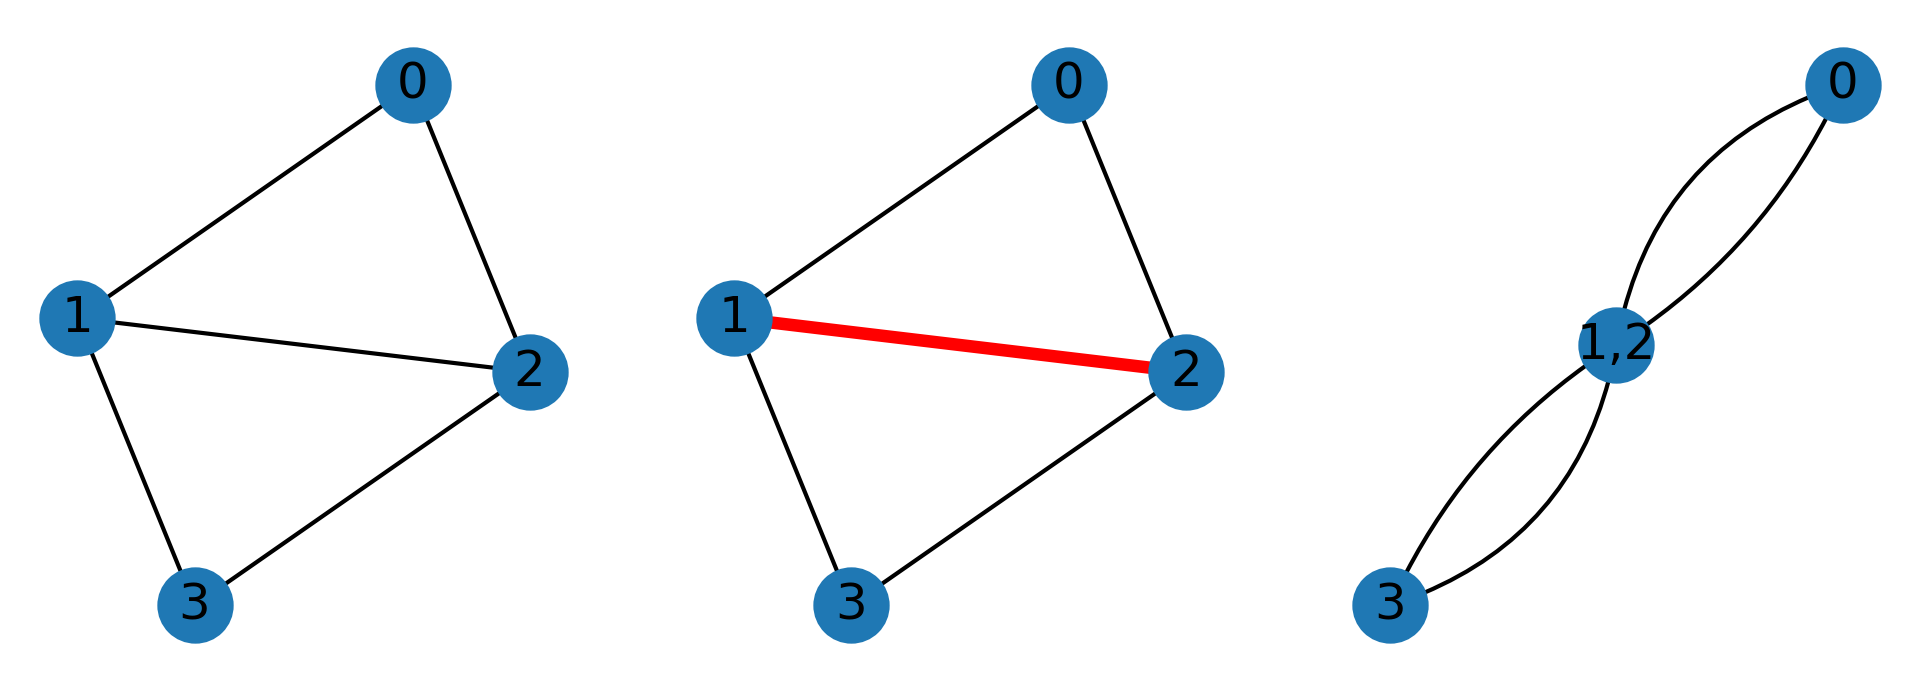
\includegraphics[width=1.0\textwidth]{figures/fig-karger-contraction.png}
    \caption{A contraction of the edge $e=(1,2)$: the original (multi)graph is on the left, and the resulting (multi)graph $G/e$ on the right.}
    \label{fig:karger:contraction}
\end{figure}

Another way to interpret the contraction is that, after contracting some edges to get a multigraph $G'=G/(e_1,\dots, e_k)$, each vertex $u$ in $G'$ corresponds to a subset of vertices $S_u\subseteq \red{V}$ from the original graph $G=(\red{V}, \orange{E})$: the subset of all vertices that were contracted together to become $u$. And any two distinct $u,v$ from $G'$ correspond to \emph{disjoint} subsets $S_v,S_v\subseteq \red{V}$ (during a contraction, a vertex cannot be merged to two separate new vertices!). 

So if after a sequence of contractions we end up with a multigraph $G'$ which has only \emph{two} vertices $u,v$, we get a cut in our original graph $G$: the cut $(S_u, S_v)$. And the value $c(S_u, S_v)$ of this cut is then exactly the number of parallel edges between $u$ and $v$. 

This is the basis for our algorithm, which we are now able to state:
\begin{algorithm}[H]
\begin{algorithmic}[1]
    \Require multigraph $G=(\red{V}, \orange{E})$
    \While{$\abs{\red{V}} > 2$}
        \State\label{alg:krager:randomedge} Pick an edge $e\in\orange{E}$ uniformly at random
        \State\label{alg:krager:result} Contract it, and let $G \gets G/e$
    \EndWhile
    \State\Return the cut defined by the remaining two vertices.
\end{algorithmic}
\caption{Karger's \textsc{Min-Cut} algorithm.}
\label{alg:karger}
\end{algorithm}
This is all. Each iteration of the loop takes time $O(\red{n})$\marginnote{The contraction operation does, and we will see in the tutorial that sampling an edge uniformly can be done in time $O(\red{n})$ as well.}; each contraction reduces the number of vertices by one, and we started with $\red{n}$ vertices: so we have $\red{n}-2$ iterations. Overall, running~\cref{alg:karger} takes $O(\red{n}^2)$ time. \emph{But is the cut it returns any good?} And importantly, \emph{why} would we expect to be any good?

\begin{figure}[htbp]
    \foreach \i in {0,1,...,10}{
    \includegraphics[scale=0.19]{figures/karger/plotgraph-\i.png} 
    }
    \caption{The sequence of steps for one run of Karger's algorithm (\cref{alg:karger}) on a (regular) graph with $\red{n}=12$ vertices and $\orange{m}=48$ edges. The cut returned has $8$ edges.}
\end{figure}

\paragraph{Some intuition.} As a thought experiment, consider any (fixed) cut $C=(A,B)$ of the graph. The only way $C$ will survive until the end of the algorithm (and be returned in~\cref{alg:krager:result}) is if we never contract any edge going from a vertex in $A$ to a vertex in $B$: that is, any vertex of the cut itself. Because as soon as we contract such an edge, some vertex in $A$ is merged with some vertex in $B$, and the cut $(A,B)$ does no longer exist in our new contracted multigraph. Put differently, the more edges there are between $A$ and $B$, the less likely the cut $C$ should be to make it to the end of the algorithm, and as a result, we expect ``small cuts'' (those with fewer edges crossing) to have a better probability to be returned.\marginnote{Consider a different strategy for~\cref{alg:krager:randomedge} of the algorithm, which would sample a pair of distinct vertices $(u,v)$ uniformly at random (not necessarily an edge). Would that work?} But that's exactly what we want: by definition, minimum cuts are the smallest cuts possible! So they should be the ones being the most likely to be returned by our algorithm\dots 

To make it formal, fix any \emph{minimum} cut $C=(A,B)$ of $G$, and let $\green{k}=c(A,B)$ be its value. For $1\leq i\leq \red{n}-2$, let $\mathcal{E}_i$ be the event that the edge $e$ picked in the $i$-th step of the algorithm does \emph{not} belong to our cut $C$. By the above discussion,
\begin{align*}
\probaOf{C\text{ is returned}} 
&= \proba[\mathcal{E}_1\cap \mathcal{E}_2\cap\dots \cap \mathcal{E}_{\red{n}-2}] \tag{No edge from $C$ is ever contracted}\\
&= \proba[\mathcal{E}_1]\probaCond{\mathcal{E}_2}{\mathcal{E}_1}\cdots\probaCond{\mathcal{E}_{\red{n}-2}}{\mathcal{E}_1\cap \mathcal{E}_2\cap\dots \cap \mathcal{E}_{\red{n}-1}}
\end{align*}
Based on this, what we need to conclude is to get a good lower bound on the probability
\[
    \probaCond{\mathcal{E}_{i+1}}{\mathcal{E}_1\cap \mathcal{E}_2\cap\dots \cap \mathcal{E}_{i}}
\]
for all $1\leq i\leq \red{n}-3$: then, we will multiply all of them, and hope for the best. Write $G_i = (\red{V}_i, \orange{E}_i)$ for the multigraph at the end of step $i$: so $G_0=G$, and $G_{\red{n}-2}$ is the $2$-vertex multigraph obtained at the end. The probability that an edge of $C$ is chosen in step $i+1$ to be contracted (if $C$ has survived until then, which is the event $\mathcal{E}_1\cap \mathcal{E}_2\cap\dots \cap \mathcal{E}_{i}$) is then equal to
\begin{equation}
            \frac{\green{k}}{|\orange{E}_{i}|}
\end{equation}
We need to (upper) bound this probability, and all we know is that:\begin{itemize}
    \item the number of vertices is $\abs{\red{V}_i} = \red{n}-i$;
    \item the value of any minimum cut of $G_i$ is $\green{k}$ (there is one cut of size $\green{k}$, our cut $C$ which survived so far; and there cannot be smaller cuts, as they would imply a smaller-than-minimum cut in the original graph $G$ as well).
\end{itemize}
The key observation is that the \emph{minimum degree} of $G_i$ must then be at least $\green{k}$. Otherwise, there would exist some vertex $u\in \red{V}_i$ with less than $\green{k}$ neighbours: choosing the cut $\{u\}, \red{V}_i\setminus\{u\}$ would give a cut in $G_i$ of size less than $\green{k}$. Using the Handshaking Lemma,\footnote{Which, importantly, also holds in (simple) multigraphs.} we have
\begin{equation}
    |\orange{E}_i| = \frac{1}{2}\sum_{v\in \red{V}_i} \deg v \geq \frac{1}{2}\abs{\red{V}_i}\cdot\green{k}
\end{equation}
or, equivalently,
\[
    \frac{\green{k}}{|\orange{E}_i|} \leq \frac{2}{\abs{\red{V}_i}} = \frac{2}{\red{n}-i}\,.
\]
This shows that
\begin{equation}
    \label{eq:karger:proba:failure:step}
    \probaCond{\mathcal{E}_{i+1}}{\mathcal{E}_1\cap \mathcal{E}_2\cap\dots \cap \mathcal{E}_{i}}
    = 1- \frac{\green{k}}{|\orange{E}_i|} \geq 1-\frac{2}{\red{n}-i}
\end{equation}
and as a result, ``multiplying all the conditional probabilities and hoping for the best'' gives
\begin{align}
\probaOf{C\text{ is returned}} 
&= \prod_{i=0}^{\ns-3} \probaCond{\mathcal{E}_{i+1}}{\mathcal{E}_1\cap\dots \cap \mathcal{E}_{i}} \notag\\
&\geq \prod_{i=0}^{\ns-3} \Paren{1-\frac{2}{\red{n}-i}} \notag\\
&= \prod_{i=0}^{\ns-3} \frac{\red{n}-i-2}{\red{n}-i} \notag\\
&= \prod_{j=3}^{\ns} \frac{j-2}{j} \notag\\
&= \frac{1\cdot 2\cdot 3\cdot 4 \cdots (\ns-2)}{3\cdot 4\cdot 5 \cdots \cdot (\ns-2)(\ns-1)\ns} \notag\\
&= \frac{2}{(\ns-1)\ns} \label{eq:karger:success:probability}\,.
\end{align}
What we showed is that, with probability at least $\frac{2}{(\ns-1)\ns}$, Karger's algorithm (\cref{alg:karger}) returns this specific minimum cut $C$. There may be more than one possible minimum cut, so the probability it returns \emph{some} minimum cut is at least $\frac{2}{(\ns-1)\ns}$:
\begin{theorem}
    \label{theo:karger}
    Karger's algorithm (\cref{alg:karger}) returns a minimum cut with probability at least $\frac{2}{(\ns-1)\ns} = \bigOmega{1/\ns^2}$.
\end{theorem}
On the one hand, this is great: the algorithm works! On the other hand, this is somewhat problematic: the probability of success we can guarantee is \emph{very} small. Fortunately, similarly to what we saw in Chapter~2, we can increase our probability of success by repetition, using~\cref{alg:karger} as a blackbox. That is:
\begin{algorithm}[H]
\begin{algorithmic}[1]
    \Require multigraph $G=(\red{V}, \orange{E})$, integer $\blue{T}$
    \For{$1\leq t\leq \blue{T}$} \!\Comment{Use fresh (independent) random bits for each}
        \State Run~\cref{alg:karger} on $G$, let $C_t$ be the output
    \EndFor
    \State\Return the smallest cut among all cuts $C_1,\dots, C_{\blue{T}}$ obtained
\end{algorithmic}
\caption{Amplifying the probability of Karger's \textsc{Min-Cut} algorithm via repetition.}
\label{alg:karger:repeated}
\end{algorithm}
From~\cref{theo:karger}, we know that each of the $\blue{T}$ independent repetitions of the algorithm has probability $p \geq \frac{2}{\ns(\ns-1)}$ of returning a minimum cut. And since it is returning the best cut among them,~\cref{alg:karger:repeated} will return a minimum cut unless \emph{none} of these $\blue{T}$ cuts is a minimum cut. So
\[
    \probaOf{\substack{\text{\cref{alg:karger:repeated} fails to}\\\text{ return a minimum cut}}} = \Paren{1-p}^{\blue{T}} \leq \Paren{1-\frac{2}{\ns(\ns-1)}}^{\blue{T}} \leq e^{-\frac{2\blue{T}}{\ns(\ns-1)}}
\]
where we used the inequality $1-x \leq e^{-x}$ in the end. To achieve probability of success $1-\errprob$, it suffices to choose $\blue{T}$ so that the RHS is at most $\errprob$: one can check that setting 
\[
    \blue{T} = \clg{\ns^2\ln(1/\errprob)}
\]
suffices. Overall, the running time is $O(\blue{T}\ns^2)$, showing the following:
\begin{theorem}
    \label{theo:karger:repeated}
    For any $\errprob>0$, the ``Best-of-$\blue{T}$'' version of Karger's algorithm (\cref{alg:karger:repeated}) returns a minimum cut with probability at least $1-\errprob$, and runs in time $\bigO{\ns^4\log(1/\errprob)}$.
\end{theorem}
Given how simple the algorithm is, this is quite remarkable! However, given that the (much more involved) best deterministic algorithm can find a minimum cut in time $O(\orange{m}\red{n}\log\frac{\ns^2}{\orange{m}}) = \bigO{\ns^3}$, it is natural to wonder if we can do even better. 

\subsection{Improving Karger’s algorithm: the Karger--Stein algorithm} The starting point is to note that Karger's algorithm does \emph{very} well in the first few iterations, but the guarantees degrade quickly towards the end. Again, let's look at a fixed minimum cut $C$ of size $\green{k}$: the probability to ``kill'' $C$ with the first contraction is very small, $\green{k}/\orange{m}$. At the $i$-th step, when $i$ is not too big, this is still very small: in~\cref{eq:karger:proba:failure:step}, we bounded it by
\[
    \frac{2}{\ns-i} \approx \frac{2}{\ns}
\]
All good! But at the \emph{end} of the algorithm, the last few steps, this becomes really, really bad: at the last step ($i=\ns-3$), for instance, the probability that $C$ is ``killed'' is only bounded by
\[
   \frac{2}{\ns-i} = \frac{2}{3} 
\]
This tells us that after surviving almost until the end, we can only guarantee that our minimum cut $C$ has a $33\%$ chance of surviving the very last step! And the first few contractions before that are not much better: each of them has a constant probability of killing $C$.

Based on this, it makes sense to only run Karger's algorithm for a while, and then do ``something else'' once we have contracted sufficiently many edges. This leaves two questions: (1)~When should we stop? and (2)~What should we do afterwards?

To answer the first question, we can look back at our analysis of the success probability. If we stop after $\ns-\blue{s}$ steps, we are left with $\blue{s}$ vertices, and similarly to what we did in~\cref{eq:karger:success:probability} we can guarantee that any fixed minimum cut survives with probability at least
\[
\prod_{i=0}^{\ns-\blue{s}-1} \frac{\red{n}-i-2}{\red{n}-i}
= \prod_{j=\blue{s}+1}^{\ns} \frac{j-2}{j}
= \frac{\blue{s}(\blue{s}-1)}{\red{n}(\red{n}-1)}
\]
If we choose $\blue{s} = \frac{\ns}{\sqrt{2}}+1$, we get
\[
    \probaOf{C \text{ survives these }\ns-\blue{s}\text{ steps}} \geq \frac{1}{2}\,.
\]
So this answers (1): we should stop once only $\frac{\ns}{\sqrt{2}}+1$ vertices remain. Then, even if there was only a single minimum cut $C$ in the original graph, it will have survived with probability at least $1/2$. But turning to question (2): what to do afterwards?\smallskip

We reduced the size of the problem by a constant factor, from $\ns$ vertices to $\approx \frac{\ns}{\sqrt{2}}$. In the absence of a better idea, this seems to call for a recursive approach.\marginnote{``When in doubt, recurse''}

First, the base case: we can only recurse if we make progress at each call, and that can only happen if
\[
    \clg{\frac{\ns}{\sqrt{2}}+1} > \ns
\]
and that is only true for $\ns \geq 7$. This gives us our base case: if $\ns \leq 6$, we will just compute a minimum cut by brute force (in constant time).

Second, $1/2$ probability is much better than $\approx 1/\ns^2$, but it is still small: for a recursive approach, dropping our probability of success by such a constant factor at each recursive step could be bad. But if we have a probability of success at least $1/2$, repeating the first stage \emph{twice} might not be a bad idea: we would have two different multigraphs $G_1,G_2$ on $\blue{s} \approx \frac{\ns}{\sqrt{2}}$ vertices, each of them (independently) still containing a minimum cut with probability at least $1/2$. ``In expectation'', at least $2\cdot (1/2)=1$ still will have a minimum cut. This gives us our algorithm, given in~\cref{alg:karger:stein}.
\begin{algorithm}[htbp!]
\begin{algorithmic}[1]
%%%%%%%%%%%%%%%%%%%%%%%%%%%%%%%%%%%%%%%%%%%%%%%%%%
\algblockdefx{BeginFirstStage}{EndFirstStage}{$\triangleright$~\textbf{Contraction}}{}
\algblockdefx{BeginSecondStage}{EndSecondStage}{$\triangleright$~\textbf{Recursion}}{}
\algtext*{EndFirstStage}% Remove "EndFirstStage" text and line
\algtext*{EndSecondStage}% Remove "EndSecondStage" text and line
%%%%%%%%%%%%%%%%%%%%%%%%%%%%%%%%%%%%%%%%%%%%%%%%%%
\Procedure{ModifiedKarger}{$G=(\red{V}, \orange{E})$, $\blue{s}$}
    \While{$\abs{\red{V}} > \blue{s}$}
        \State Pick an edge $e\in\orange{E}$ uniformly at random
        \State Contract it, and let $G \gets G/e$
    \EndWhile
    \State\Return $G$
\EndProcedure
\Procedure{KargerStein}{$G=(\red{V}, \orange{E})$}
    \If{$\abs{\red{V}} \leq 6$}
        \State \Return a minimum cut \Comment{Brute-force computation}
    \EndIf
    \State Set $\blue{s} \gets \clg{{\ns}/{\sqrt{2}}+1}$
    \BeginFirstStage
        \State $G_1 \gets \textsc{ModifiedKarger}(G,\blue{s})$
        \State $G_2 \gets \textsc{ModifiedKarger}(G,\blue{s})$
    \EndFirstStage
    \BeginSecondStage
        \State $C_1 \gets \textsc{KargerStein}(G_1)$
        \State $C_2 \gets \textsc{KargerStein}(G_2)$
    \EndSecondStage
    \State\label{alg:karger:stein:return}\Return the smallest cut among $C_1,C_2$
\EndProcedure
\end{algorithmic}
\caption{The Improved Karger--Stein \textsc{Min-Cut} algorithm.}
\label{alg:karger:stein}
\end{algorithm}
To analyse this \textsc{KargerStein} algorithm, we need to establish its running time $T(\ns)$ and its probability of success $p(\ns)$. The running time turns out to be the simplest: we have two calls to \textsc{ModifiedKarger}, which (as in~\cref{alg:karger}) each take time $O(\ns^2)$; following by two recursive calls on instances of size $\blue{s}\approx \ns/\sqrt{2}$. Ignoring the ceiling for simplicity, this gives the recurrence relation
\begin{equation}
    T(\ns) = 2T(\ns/\sqrt{2})+O(\ns^2)
\end{equation}\marginnote{Verify it, \eg with the Master Theorem; or, even better, without it.}
which solves to $\boxed{T(\ns)=O(\ns^2\log\ns)}$ \emph{via} the standard techniques.\medskip

The probability of success $p(\ns)$ is trickier. From our setting of $\blue{s}$, we know that $G_1$ still contains a minimum cut with probability at least $1/2$: whenever that happens, $C_1$ will be a minimum cut if the recursive call to \textsc{KargerStein} is successful, which itself happens with probability at least $p(\ns/\sqrt{2})$. That is,
\[
    \probaOf{C_1\text{ is a minimum cut}} \geq \frac{1}{2}\cdot p\Paren{\frac{\ns}{\sqrt{2}}}
\]
Similarly, looking at $G_2$ we have $\probaOf{C_2\text{ is a minimum cut}} \geq \frac{1}{2}\cdot p({\ns}/\sqrt{2})$. Since we are taking the best of $C_1,C_2$ on~\cref{alg:karger:stein:return}, the algorithm succeeds unless \emph{neither} of $C_1,C_2$ is a minimum cut:
\begin{align*}
p(\ns) &= 1-\Paren{1-\probaOf{C_1\text{ is a minimum cut}}}\Paren{1-\probaOf{C_2\text{ is a minimum cut}}} \\
&\geq 1-\Paren{1-\frac{1}{2} p\Paren{\frac{\ns}{\sqrt{2}}}}^2
\end{align*}
We are left with the task of solving this recurrence relation on $p(\ns)$, with the base cases $p(\ns) = 1$ for $\ns\leq 6$. 
\begin{claim}[\advancedstuff]
    The recurrence relation
    \[
       p(\ns) \geq 1-\Paren{1-\frac{1}{2} p\Paren{\frac{\ns}{\sqrt{2}}}}^2
    \]
    has solution $p(\ns) = \bigOmega{1/\log\ns}$.
\end{claim}
\begin{proof}
    Write $\ns = \sqrt{2}^t$ for $t\geq 1$.
    Expanding the square, this boils down to analysing the recurrence relation
    \[
        p(\sqrt{2}^t) \geq p(\sqrt{2}^{t-1}) - \frac{1}{4}p(\sqrt{2}^{t-1})^2
    \]
    or, equivalently (reparameterizing by setting $f(t) = p(\sqrt{2}^t)\in[0,1]$),
    \begin{equation}
        f(t) \geq f(t-1)-\frac{1}{4}f(t-1)^2\,.
    \end{equation}\marginnote{\advancedstuff{} Another ``rabbit-out-of-the-hat'' proof: set $g(t) = \frac{4}{f(t)}-1$, and substitute in the inequality. Solve the resulting inequality.}
    Note that the function $x\mapsto x-\frac{1}{4}x^2$ is increasing on $[0,1]$: this will come handy later. We will show by induction on $t$ that $f(t) \geq \frac{1}{t+2}$.
    \begin{itemize}
        \item This is true for $t=0$, since $f(0) = p(1)=1$.
        \item Assuming it is true for $t-1$, we have
        \begin{align*}
        f(t) &\geq f(t-1)-\frac{1}{4}f(t-1)^2 \\
        &\geq \frac{1}{t+1}-\frac{1}{4}\Paren{\frac{1}{t+1}}^2 \tag{induction hypothesis and $x\mapsto x-\frac{1}{4}x^2$ increasing} \\
        &= \frac{4t+3}{4(t+1)^2} = \frac{1}{t+2} + \frac{3t+2}{4(t+1)^2(t+2)} \\
        &\geq \frac{1}{t+2}
        \end{align*}
        concluding the induction proof.
    \end{itemize}
    Recalling that $\ns = \sqrt{2}^t$, we have $t = 2\log\ns$, and the above shows that $p(\ns) \geq \frac{1}{2\log\ns+2} = \bigOmega{\frac{1}{\log\ns}}$, as claimed.
\end{proof}
\noindent What we have shown can be summarised as follows:
\begin{theorem}
    \label{theo:karger:stein}
    The Karger--Stein algorithm (\cref{alg:karger:stein}) runs in time $O(\ns^2\log\ns)$, and returns a minimum cut with probability at least $\bigOmega{1/\log\ns}$.
\end{theorem}
Moreover, with exactly the same approach as\marginnote{Exercise: prove it!} for~\cref{theo:karger:repeated} (using~\cref{theo:karger:stein} and setting $\blue{T} = O(\log\ns\cdot \log(1/\errprob))$), we get
\begin{corollary}
    \label{theo:karger:stein:repeated}
    For any $\errprob>0$, the ``Best-of-$\blue{T}$'' version of the Karger--Stein algorithm returns a minimum cut with probability at least $1-\errprob$, and runs in time $\bigO{\ns^2\log^2\ns \log(1/\errprob)}$.
\end{corollary}
This is now typically \emph{much} faster than the $\bigO{\orange{m}\red{n}\log\frac{\red{n}^2}{\orange{m}}}$ running time of the deterministic algorithm!\marginnote{Specifically, as long as the graph is even mildly dense, \ie $\orange{m} \gg \ns\log\ns$.}

\begin{remark}
    There is a different deterministic algorithm, due to Stoer and Wagner~\cite{StoerW97} and not based on computing maximum flows, with the running time $\bigO{\orange{m}\red{n}+\red{n}^2\log\red{n}}$ (slightly better than $\bigO{\orange{m}\red{n}\log\frac{\red{n}^2}{\orange{m}}}$, but still worse than~\cref{theo:karger:repeated}). Interestingly, this algorithm also works by performing some type of contraction (merging two carefully selected vertices at each step).
\end{remark}

\subsection{How many minimum cuts are there?}
The \textsc{Min-Cut} question we have considered so far asks to \emph{find} a minimum cut in a graph $G$: \emph{any} minimum cut. There is always at least \emph{one} minimum cut, but could there be more? How many, at most?
\begin{itemize}
    \item $\Theta(\ns)$?
    \item $\Theta(\ns^2)$?
    \item $\Theta(2^{\ns})$?
    \item Something else?
\end{itemize}
And \emph{how to prove it}?\medskip

Fortunately, we already have the answer, \emph{and} done the proof. We just did not realise it at the time! This is a beautiful example where analysing an algorithm establishes a structural result, almost ``as a side effect.''

Taking a step back: in order to prove~\cref{theo:karger}, we have shown that if $C$ is a minimum cut of $G$, then~\cref{alg:karger} outputs $C$ with probability at least
\[
    \frac{2}{\ns(\ns-1)} = \frac{1}{\binom{\ns}{2}}
\]
This means that if there exists $\green{M}$ distinct minimum cuts in the graph $G$, the probability to output one of them is at least
\[
    \probaOf{ \substack{\textsc{Karger}(G)\text{ outputs}\\\text{one of } C_1,\dots, C_{\green{M}}}} = \sum_{i=1}^{\green{M}} \probaOf{ \textsc{Karger}(G)\text{ outputs } C_i} \geq \frac{\green{M}}{\binom{\ns}{2}}
\]
But probabilities are at most one, so $\probaOf{ \substack{\textsc{Karger}(G)\text{ outputs}\\\text{one of } C_1,\dots, C_{\green{M}}}}\leq 1$. Which means that
\[
    \green{M} \leq \binom{\ns}{2}
\]
and we get the following ``for free'':
\begin{theorem}
    An undirected graph $G=(\red{V},\orange{E})$ on $|\red{V}|=\ns$ vertices has at most $\binom{\ns}{2}$ minimum cuts.
\end{theorem}
This is quite surprising, since every\marginnote{Do you see why?}  graph on $\ns$ vertices has exactly $2^{\ns-1}-1$ distinct (not necessarily minimum) cuts. As usual, we can ask whether this $\binom{\ns}{2}$ bound is tight: and the answer is \emph{yes}, as there exist some $\ns$-vertex graphs with that many minimum cuts. A simple example is a cycle on $\ns$ vertices, where choosing any $2$ edges out of $\ns$ defines a distinct minimum cut: see~\cref{fig:cycle:graph}.
\begin{figure}[htbp]
    \centering
    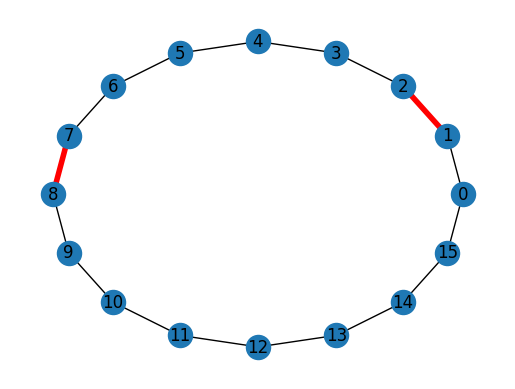
\includegraphics[width=0.9\textwidth]{figures/fig-cyclegraph}
    \caption{The cycle graph $C_{16}$ on $16$ vertices, along with a specific (mininum) cut (defined by the two \red{red} edges). Any choice of two edges creates a different minimum cut of the graph: there are $\binom{16}{2}$ such choices.}
    \label{fig:cycle:graph}
\end{figure}

%%%%%%%%%%%%%%%%%%%%%%%%%%%%%%%%%%%%%%%%%%%%%
\section{Minimum Spanning Tree in Expected Linear Time}
Another classic and fundamental graph problem is the \emph{minimum spanning tree} one, which, given a connected weighted graph $G$, asks to find a spanning tree\marginnote{A \emph{spanning tree} of a graph $G$ is a connected subgraph of $G$ with no cycle. A \emph{spanning forest} is the same thing without the requirement to be connected.} with minimum total weight:\marginnote{A \emph{minimum spanning forest} (MSF) is the equivalent of an MST when the graph is not connected: it asks for a collection of MSTs, one for each connected component of the graph.}
\begin{framed}
\noindent \textsc{Minimum Spanning Tree (MST)}: Given an (undirected) connected graph $G=(\red{V},\orange{E})$ on $\red{n}$ vertices and $\orange{m}$ edges with positive weights $\purple{w}\colon \orange{E}\to \R_+$, output a spanning tree $T$ minimising $\purple{w}(T) = \sum_{e\in T} \purple{w}(e)$.
\end{framed}
As in the previous section, you most likely remember from previous algorithms class that \emph{we have deterministic algorithms to solve this efficiently:}
\begin{itemize}\marginnote{$\log^\ast$ is the iterated logarithm, an incredibly slow-growing function defined as ``the number of times one must apply the logarithm to reach a value at most $1$:''
    \[
        \log^\ast x = \begin{cases}
            0&\text{if } x \leq 1\\
            1+\log^\ast\log x& \text{otherwise.}
        \end{cases}
    \]
    $\log^\ast n$ still goes to infinity as $n$ grows, but \emph{very} slowly.}
    \item Kruskal's algorithm solves it in time $\bigO{\orange{m}\log\red{n}}$
    \item Prim's algorithm solves it in time $\bigO{\orange{m}\log\red{n}}$ when implemented with a heap, or, better, $\bigO{\orange{m} + \red{n}\log\red{n}}$ using a Fibonacci heap
    \item Bor\r{u}vka's algorithm solves it in time $\bigO{\orange{m}\log\red{n}}$
    \item the Fredman--Tarjan algorithm solves it in time $\bigO{\orange{m}\log^\ast\red{n}}$
    \item Chazelle's algorithm solves it in time $\bigO{\orange{m}\alpha(\orange{m},\red{n})}$\marginnote{$\alpha$ is the \emph{inverse Ackermann function}, which grows \emph{even slower}.}
\end{itemize}
The key point is that these algorithms (or their analysis) get more and more involved as we go down the list, and that \emph{no deterministic algorithm running in linear time (that is, $O(\orange{m})$) is known.}\medskip

There is, however, a \emph{randomised} algorithm for MST running in \emph{expected} linear time, due to Karger, Klein, and Tarjan~\cite{KargerKT95}. We will not go through its description and analysis in detail, but will only provide the key building blocks. 

From now on, we will assume for convenience that all the weights $\{\purple{w}(e)\}_{e\in\orange{E}}$ are distinct. This is to make sure we can break ties consistently, and is without loss of generality.\marginnote{A standard way to implement consistent tie-breaking when some weights are equal is to do so using the lexicographic order of the edges.} One nice consequence of this assumption is that the MST is now \emph{unique}: there can be only one!\marginpar{Can you see why?}\medskip

The main idea behind the algorithm can be summarized like this:
\begin{framed}
    \noindent If we had a way to remove most edges from $G$ \emph{without affecting its MST}, then we could recurse on a much sparser graph $G'$.
\end{framed}
The question here is \emph{how} to efficiently remove ``most edges'' (in expectation) without killing the MST in the process.

The first building block we need to answer this are the \emph{cut} and \emph{cycle} properties, which underly the proof (and ideas) behind Prim's and Bor\r{u}vka's algorithm (cut property), and Kruskal's algorithm (cycle property):
\begin{framed}
\noindent\textbf{Cut property.} Let $S\subseteq \red{V}$ be any subset of vertices, and let $e$ be the minimum-weight edge with exactly one endpoint in $S$. Then the MST of $G$ contains $e$.
\end{framed}
\begin{framed}
\noindent\textbf{Cycle property.} Let $C\subseteq \orange{E}$ be any cycle, and let $e$ be the maximum-weight edge belonging to $C$. Then the MST of $G$ does not contain $e$.
\end{framed}
We will require the definition of an edge being ``heavy'' with respect to a forest:
\begin{definition}
    For any weighted graph $G=(\red{V}, \orange{E})$ and forest $F\subseteq\orange{E}$ of $G$, we say that an edge $e\in \orange{E}\setminus F$ is \emph{$F$-heavy} if (1)~adding $e$ to $F$ creates a cycle, and (2)~$e$ is the maximum-weight edge of that cycle.
\end{definition}
\noindent From the cycle property, we readily get the following fact:
\begin{framed}
\noindent\textbf{$F$-heaviness property.} Let $F\subseteq \orange{E}$ be a forest of $G$, and let $e\in \orange{E}\setminus F$ be an \emph{$F$-heavy} edge. Then the MST of $G$ does not contain $e$.
\end{framed}
This looks promising: what this says is that if we have a forest (any forest!) $F$ of $G$, we can safely remove all $F$-heavy edges from $G$ without killing the MST. This sounds exactly like what we are hoping for! Provided, of course, that we can (1)~efficiently find all $F$-heavy edges, and (2)~that there are \emph{many} of them.\smallskip

\noindent The second building block ensures that, at least, we can do (1):
\begin{fact}
    \label{fact:verification:mst}
    There exists a deterministic algorithm $\textsc{MSTVerification}$~\cite{DixonRT92}\cite{King97} which, on input a graph $G=(\red{V}, \orange{E})$ with weights $\purple{w}$ and a forest $F$ of $G$, outputs the set of $F$-heavy edges of $G$ in time $O(\orange{m}+\red{n})$.\marginnote{This type of algorithms is typically used to check whether a given tree is really an MST, hence the name ``MST Verification.''}
\end{fact}

To third and last building blocks will take care of (2). The idea here is that we \emph{already} had the MST $T$ (which we can see as a forest), then by the cycle property \emph{every} edge $e\in G\setminus T$ is $T$-heavy: and so we could use~\cref{fact:verification:mst} on $T$ to find (and remove) $\orange{m}-\red{n}+1$ edges from $G$ in time $O(\orange{m}+\red{n})$. That would be amazing progress~--~but of course, \emph{we do not have $T$}, that's the thing we are trying to compute!

What we \emph{could} do, however, is computing the MST $T'$ of a small random subgraph $G'$ of $G$, and use that as our ``guiding forest'' to find which heavy edges to remove from $G$. If $G'$ has sufficiently few edges and vertices (for instance, $\orange{m}/2$ and $\red{n}/2$) then we can compute its MST $T'$ recursively. So to do that, we need to ``sparsify'' $G$: both in terms of vertices and edges. 

For the edges, this is easy: given a graph $G=(\red{V}, \orange{E})$, we can build a new graph $G'$ with (in expectation) much fewer edges by keeping each edge of $\orange{E}$ independently with probability $\blue{p}\in[0,1]$: this gives us $G'=(\red{V}, \orange{E'})$ with $\expect{|\orange{E'}|} = \blue{p}|\orange{E}|$. Our third building block tells us what happens to the MST\footnote{Or, rather, maximum spanning forest (MSF), since randomly removing some edges might have disconnected $G'$.} when we do that: is the MSF of $G'$ still ``good''?
\begin{lemma}[Random Subsampling Lemma]
    \label{lemma:graph:random:sampling:mst}
    Let $G'=(\red{V}, \orange{E'})$ be a subgraph of $G=(\red{V}, \orange{E})$ obtained by subsampling each edge $e\in\orange{E}$ independently with probability $\blue{p}\in[0,1]$, and $F\subseteq \orange{E'}$ be the MSF of $G'$. Then the expected number of edges \emph{in $G$} that are not $F$-heavy is at most
    $
        \frac{|\red{V}|}{\blue{p}}
    $.
\end{lemma}
We leave the proof of this lemma as an exercise.\marginnote{\advancedstuff{} Exercise!} The crucial part of the statement is that we compute $F$ as the MSF of the \emph{sparser} graph $G'$ but get a guarantee on the number of $F$-heavy edges with respect to the \emph{original} graph $G$.\smallskip

To sparsify $G$ in terms of vertices, the last building block we need is Bor\r{u}vka's algorithm, or, rather, what happens when we run it only for a couple iterations: \cref{alg:boruvka:step}.
\begin{algorithm}[htbp!]
\begin{algorithmic}[1]
\Procedure{BoruvkaStep}{$G=(\red{V}, \orange{E})$, $\blue{t}$}
    \State $F\gets \emptyset$ \Comment{$F$ stands for ``Forest''}
    \For{$1\leq i\leq\blue{t}$}
        \ForAll{$v\in\red{V}$}
            \State Find the lightest edge $e\in\orange{E}$ incident to $v$:
            \[
            e\gets \arg\!\min\{\purple{w}(v,u): (v,u)\in\orange{E}\}
            \]
            \State Contract it, and let $G \gets G/e$
            \State $F\gets F\cup\{e\}$ \Comment{Add it to $F$}
        \EndFor
        \ForAll{$u,v\in \red{V}$} \Comment{In the new graph}
            \If{$u,v$ are connected by more than one edge}
                \State only keep one with the smallest weight
            \EndIf
        \EndFor
    \EndFor
    \State\Return $(G, F)$ \Comment{New graph and forest of contracted edges}
\EndProcedure
\end{algorithmic}
\caption{$\blue{t}$-step version of Bor\r{u}vka's algorithm}
\label{alg:boruvka:step}
\end{algorithm}
\begin{lemma}
    \label{lemma:boruvska:step}
    The $\blue{t}$-step version of Bor\r{u}vka's algorithm, on input a connected graph $G=(\red{V}, \orange{E})$, returns a new graph $G'=(\red{V'}, \orange{E'})$ such that $|\red{V'}| \leq {|\red{V}|}/{2^{\blue{t}}}$, and runs in time $O(\blue{t}\cdot \orange{m})$.
\end{lemma}
\begin{proof}[Proof sketch]
Each step can be implemented to run in time $O(\orange{m})$; and at each step, each vertex is contracted with at least one other, so the total number of vertices decreases by at least a factor $2$.
\end{proof}

\marginnote{Here $\blue{t}\geq 1, \blue{p}\in[0,1]$ are parameters we will get to choose for things to work out.}At this point, we finally have all we need for the algorithm. To summarise our strategy:
\begin{enumerate}
    \item Sparsify $G$ in terms of vertices, to go from $\ns$ to $\ns' = \ns/2^{\blue{t}}$:\marginnote{One can check that adding $F_1$ to an MSF of $G_1$ gives the MST of $G$, so it remains to find an MSF of $G_1$.} this gives a graph $G_1$ on $\ns'$ vertices (and a leftover forest $F_1$ of contracted edges)
    \item\label{step:random:subsampling:mst} Sparsify $G_1$ in terms of edges, to go from $\orange{m}$ to $\orange{m}' \leq \blue{p}\orange{m}$ (in expectation: this is the only random step): this gives a graph $G_2$ on $\ns'$ vertices and $\orange{m}'$ edges
    \item Recursively find the MSF $F_2$ of $G_2$: this should be less expensive, as $G_2$ is smaller than $G$
    \item Find all the $F_2$-heavy edges in $G_1$, and remove them from $G_1$ to get a graph $G_3$: there should be many by~\cref{lemma:graph:random:sampling:mst}, and can be done efficiently by~\cref{fact:verification:mst}
    \item Recursively find the MSF $F_3$ of $G_3$: this should be less expensive, as $G_3$ is smaller than $G$: and this is also the MSF of $G_1$
    \item return $T=F_1\cup F_3$ as the MST of $G$
\end{enumerate}\marginnote{\emph{If} we are lucky, we remove many edges and get $\orange{m}' \ll \orange{m}$ and also end up with many $F_3$-heavy edges, so the recursive calls will be faster. If we are unlucky, the recursive calls will be on bigger graphs, and so will be slower.}
It is worth pointing out that the only random step in the above strategy is Step~\ref{step:random:subsampling:mst}, and it does not affect \emph{correctness}: it only affects the running time.\smallskip

\noindent We can finally state the algorithm itself:
\begin{algorithm}[htbp!]
\begin{algorithmic}[1]
\Procedure{Subsample}{$G=(\red{V}, \orange{E})$, $\blue{p}$}
    \State $\orange{E'} \gets \emptyset$
    \ForAll{$e\in\orange{E}$} \Comment{Independently for each edge}
        \State Add $e$ to $\orange{E'}$ with probability $\blue{p}$
    \EndFor
    \State\Return $G'=(\red{V}, \orange{E'})$
\EndProcedure
\Procedure{LinearTimeMST}{$G=(\red{V}, \orange{E})$, $\blue{t}$, $\blue{p}$}
    \If{$\abs{\red{V}} \leq 2$}
        \Return $G$ \Comment{Base case}
    \EndIf
    \State $G_1 \gets \textsc{BoruvkaStep}(G,\blue{t})$ \label{step:kkt:boruvska}
    \State $G_2 \gets \textsc{Subsample}(G_1,\blue{p})$ \label{step:kkt:subsampling}
    \State $F_2 \gets \textsc{LinearTimeMST}(G_2,\blue{t},\blue{p})$ \Comment{Recursive call}
    \State $H\gets \textsc{MSTVerification}(F_2, G_1)$ \Comment{Find $F_2$-heavy edges} \label{step:kkt:verification}
    \State $G_3 \gets (\red{V_1}, \orange{E_1}\setminus H)$ \Comment{Remove them from $G_1$} \label{step:kkt:pruning}
    \State $F_3 \gets \textsc{LinearTimeMST}(G_3,\blue{t},\blue{p})$ \Comment{Recursive call}
    \State\Return $F_1\cup F_3$
\EndProcedure
\end{algorithmic}
\caption{The Karger--Klein--Tarjan (KKT) Algorithm: MST in expected linear time}
\label{alg:kkt:algorithm}
\end{algorithm}
To analyse it, we need to establish its correctness and expected running time. We will only do the second, as correctness follows from the discussion and lemmas above.\footnote{Please check and establish it, this is a good exercise.}

The expected running time $T(\orange{m},\red{n})$ can be decomposed into the time taken by~\cref{step:kkt:boruvska,step:kkt:verification,step:kkt:pruning}, which by~\cref{fact:verification:mst,lemma:boruvska:step} take total time $O(\orange{m}+\red{n})+O(\blue{t}\orange{m}) = O(\blue{t}(\orange{m}+\red{n}))$; and the time of the two recursive calls, which take time $T(|\orange{E_2}|, |\red{V_2}|) + T(|\orange{E_3}|, |\red{V_3}|)$. Now, $|\red{V_1}|=|\red{V_2}|=|\red{V_3}| \leq \ns/2^{\blue{t}}$ by~\cref{lemma:boruvska:step}, and this is deterministic (comes from the Bor\r{u}vka step); but $|\orange{E_2}|$ and $|\orange{E_3}|$ are random.\marginnote{$|\orange{E_1}|\leq \orange{m}$ but is not necessarily equal to $\orange{m}$, as the Bor\r{u}vka step might have (deterministically) removed a few edges during the contractions.} All we know is that 
\begin{equation}
\label{eq:kkt:bound:expect:E2}
\expect{|\orange{E_2}|}=\blue{p}|\orange{E_1}| \leq \blue{p}\orange{m}
\end{equation}
because of subsampling, and that by~\cref{lemma:graph:random:sampling:mst,lemma:boruvska:step}
\begin{equation}
\label{eq:kkt:bound:expect:E3}
\expect{|\orange{E_3}|} \leq \frac{|\red{V_1}|}{\blue{p}} \leq \frac{\ns}{\blue{p}2^{\blue{t}}}\,.
\end{equation}
So we have, for some absolute constant $C>0$, that
\begin{equation}
    \label{eq:kkt:recurrence}
T(\orange{m},\red{n}) \leq C\cdot \blue{t}(\orange{m}+\red{n})
+ \expect{T(|\orange{E_2}|, |\red{V_2}|)} + \expect{T(|\orange{E_3}|, |\red{V_3}|)}
\end{equation}
where the expectation is over the randomness of the subsampling of the edges (\cref{step:kkt:subsampling}). Let us show by induction that
\[
    T(\orange{m},\red{n}) \leq C'\cdot (\orange{m}+\red{n})
\]
for some suitable constant $C'>0$. The base case is easy, since~\cref{alg:kkt:algorithm} runs in constant time for $\red{n} \leq 2$ (our recursive base case). Now, for the induction, assume this holds for all $(\orange{m},\red{n})$ with $\orange{m'} < \red{m}$ and $\red{n'} < \red{n}$:~\cref{eq:kkt:recurrence} gives
\begin{align}
    T(\orange{m},\red{n})
    &\leq C \blue{t}(\orange{m}+\red{n})
+ \expect{C'(|\orange{E_2}| + |\red{V_2}|)} + \expect{C'(|\orange{E_3}| + |\red{V_3}|)} \notag\\
&\leq C \blue{t}(\orange{m}+\red{n})
+ C'\Paren{\expect{|\orange{E_2}|} + \frac{\red{n}}{2^{\blue{t}}} + \expect{|\orange{E_3}|} + \frac{\red{n}}{2^{\blue{t}}} } \tag{Bound on $|\red{V_2}|,|\red{V_3}|$} \notag\\
&\leq C \blue{t}(\orange{m}+\red{n})
+ C'\Paren{\blue{p}\orange{m} + \frac{\red{n}}{\blue{p}2^{\blue{t}}} + \frac{2\red{n}}{2^{\blue{t}}} } \tag{\cref{eq:kkt:bound:expect:E2,eq:kkt:bound:expect:E3}} \notag\\
&= (C \blue{t}+C'\blue{p})\orange{m} + \Paren{C \blue{t}+C'\frac{2+1/\blue{p}}{2^{\blue{t}}}}\red{n} \label{eq:kkt:recurrence:induction}
\end{align}\marginnote{Check what happens for other choices of $\blue{t}$ and $\blue{p}$: for instance, can you choose $\blue{t}=2$? (This corresponds to only doing two rounds of the Bor\r{u}vka step.) What about $\blue{t}=1$?} %% Comment: for t=2, yes: p = (1+sqrt(5))/4 ~= 0.8 then works. Not t=1.
One can check that setting $\blue{t}=3$, $\blue{p}=1/2$,~\cref{eq:kkt:recurrence:induction} becomes
\begin{align*}
    T(\orange{m},\red{n})
&\leq (3C+C'/2)( \orange{m}+ \red{n} )
\end{align*}
which gives $T(\orange{m},\red{n}) \leq C' ( \orange{m}+ \red{n} )$ as long as $C' \geq 6C$. This concludes the proof by induction, and the proof of the theorem:\footnote{Modulo the parts we left as an exercise.}
\begin{theorem}
    \label{theo:kkt}
    The Karger--Klein--Tarjan algorithm (\cref{alg:kkt:algorithm}) computes a minimum spanning tree (MST) of an $\red{n}$-vertex, $\orange{m}$-edge undirected connected graph in \emph{expected} $\bigO{\orange{m}}$ time.
\end{theorem}
\noindent To conclude, one last thing left as an exercise: can you convert this Las Vegas algorithm into a high-probability Monte-Carlo one?

\chapter{Lecture 6: Hashing and Friends}
For the next two chapters, we will depart a little from the previous focus which was by and large on \emph{algorithms}, and look into their usual companion: \emph{data structures}. This is not saying there will not be algorithms, or analysis of algorithms, or extensive use of these concentration inequalities and mathematical notions we introduced and went over at great length! 

First, just so that we are clear on \emph{what} a data structure is: it is a way to store and organize data while providing a set of methods to access (and, usually,  update) this data \emph{efficiently}. This set of methods is the interface to the data (the analogue of an API), and you may have seen it referred in previous courses by what is called an \emph{abstract data type} (ADT). So an ADT specifies an ``API to the data,'' and a data structure is a concrete implementation of this API.\footnote{Not an implementation in terms of code, but in terms of algorithms, etc. Once you have a data structure defined and you've analyzed it, it still remains to code it at some point\dots}

Second, we will typically care about time efficiency, but also space (memory) efficiency of a data structure: if we currently store 5 $\green{m}$-bit strings, we would rather avoid using $\Theta(2^{\green{m}})$ bits of memory~--~even though in this case that's the size of the ``universe'' the data comes from (there are $2^{\green{m}}$ distinct $\green{m}$-bit strings). To quantify this, let's introduce some notation: we will have $\ns$ \emph{elements} (data points), each of them coming from a \emph{universe} (set of all possible data points) $\cX$ of size $\green{m}$. Our two main parameters will be $\ns$ and $\green{m}$: $\ns$ can increase or decrease as we add or remove elements from our data structure, and we usually have $\ns \ll \green{m}$ (the universe is big, our dataset is much smaller).

As an example: we want to store 10,000 high-resolution pictures, each 12.5 MP ($3072 \times 4080$ resolution). Assuming 8 bits per pixel, what would be the corresponding values of $\ns$ and $\green{m}$?\marginnote{This is a very naive way to bound $\green{m}$, as not all sets of pixels will be valid images. But it is good enough as a first approximation.}
\begin{itemize}
    \item $\ns=10,000$ and $\green{m} = 12,533,760$?
    \item $\ns=10,000$ and $\green{m} = 100,270,080$?
    \item $\ns=10,000$ and $\green{m} = 2^{100,270,080}$?
\end{itemize}
Clearly, we do not want to use space proportional to $\green{m}$.\medskip

Now, one of the most basic and fundamental examples of ADTs is that of the \emph{dictionary},\marginnote{Or \emph{map}, or \emph{associative array.}} which only requires to provide 3 operations to maintain a set $S\subseteq \cX$:
\begin{framed}
    \begin{itemize}
        \item$\textsc{Insert}(x)$: insert the element $x$ to $S$ (do nothing if it is already in $S$)
        \item$\textsc{Lookup}(x)$: return whether $x\in S$
        \item$\textsc{Remove}(x)$: remove the element $x$ from $S$ (do nothing if it is not in $S$)
    \end{itemize}
\end{framed}
Of course, there are several options to implement this, and you most likely have seen or easily come up with a few data structures for that:\marginnote{Check how you would get these. Can you think of others?}
\begin{itemize}
    \item A linked list! Space $O(\ns \log \green{m})$, all three operations in (worst-case) time $O(\ns)$.
    \item An array! Space $O(\green{m})$, all three operations in (worst-case) time $O(1)$.
    \item A self-balancing binary search tree (BST), \eg an AVL tree! Space $O(\ns \log \green{m})$, all three operations in (worst-case) time $O(\log\ns)$.
\end{itemize}
Each of these has its drawbacks, especially the first two. Is there a way to do better? Specifically, can we do space $O(\ns)$ \emph{and} all three operations in time complexity $O(1)$?\medskip

\noindent Not quite, but \emph{almost}. Enter {hash tables}, which, at a high level, use randomization to make the array-based approach much more space-efficient. 
\section{Hash tables}
The basic idea of hash tables is that ``the universe is a big place, but it's mostly empty.'' So if we could ``map'' our universe $\cX$ to a much, much smaller set $\cY$ such that any subset $S\subseteq \cX$ of $\ns$ distinct elements gets mapped to a subset $S'\subseteq \cY$ \emph{still} of $\ns$ distinct elements, we would be in good shape: then, we could apply the array-based solution above to $\cY$, only paying space proportional $\green{m'} = |\cY| \ll \green{m}$. Ideally, we could even take $\green{m'} = O(\ns)$?\marginnote{Sanity check: we cannot hope for $\green{m'} < \ns$. Can you see why?}



%%%%%%%%%%%%%%%%%%%%%%%%%%%%%%%%%%%%%%%%%%%%%%%%%%%%%%%%%%%%%%%%%%%%%%%%%%%
%%%%%%%%%%%%%%%%%%%%%%%%%%%%%%%%%%%%%%%%%%%%%%%%%%%%%%%%%%%%%%%%%%%%%%%%%%%
\begin{figure}
\tikzset{every picture/.style={line width=0.75pt}} %set default line width to 0.75pt     
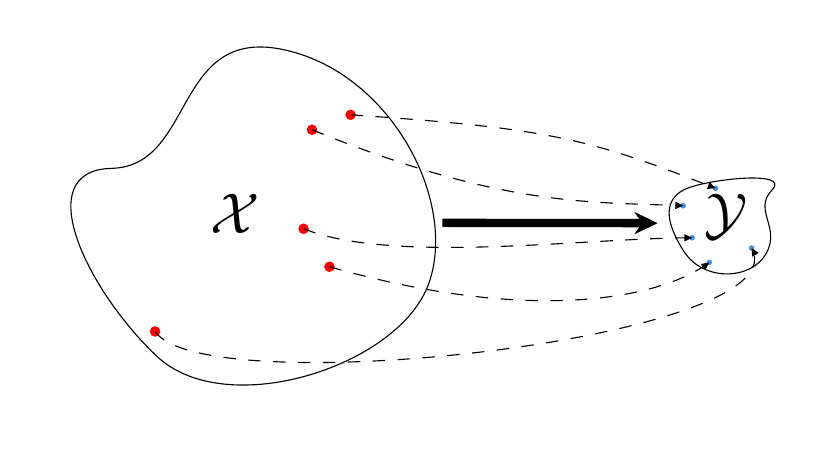
\begin{tikzpicture}[x=0.75pt,y=0.75pt,yscale=-0.6,xscale=0.6]
%uncomment if require: \path (0,300); %set diagram left start at 0, and has height of 300

%Shape: Regular Polygon [id:dp7047826808938766] 
\draw   (505.82,128.5) .. controls (521.58,120.27) and (592.49,112.04) .. (576.73,128.5) .. controls (560.97,144.97) and (583.82,158.14) .. (572,179.54) .. controls (560.18,200.94) and (521.58,202.58) .. (505.82,177.89) .. controls (490.06,153.2) and (490.06,136.74) .. (505.82,128.5) -- cycle ;
%Shape: Regular Polygon [id:dp28457392595956066] 
\draw   (182.32,15.52) .. controls (268.72,32.31) and (324.31,135.62) .. (301.3,202.88) .. controls (278.28,270.15) and (138.47,314.59) .. (82.84,262.29) .. controls (27.2,209.99) and (-20.63,112.91) .. (46.25,111.25) .. controls (113.13,109.59) and (95.91,-1.27) .. (182.32,15.52) -- cycle ;
%Straight Lines [id:da7059819659741645] 
\draw [line width=3]    (312,155) -- (478.75,155.24) ;
\draw [shift={(484.75,155.25)}, rotate = 180.08] [fill={rgb, 255:red, 0; green, 0; blue, 0 }  ][line width=0.08]  [draw opacity=0] (18.75,-9.01) -- (0,0) -- (18.75,9.01) -- (12.45,0) -- cycle    ;
%Shape: Circle [id:dp8333984030915326] 
\draw  [draw opacity=0][fill={rgb, 255:red, 255; green, 0; blue, 0 }  ,fill opacity=1 ] (196.25,159.75) .. controls (196.25,157.4) and (198.15,155.5) .. (200.5,155.5) .. controls (202.85,155.5) and (204.75,157.4) .. (204.75,159.75) .. controls (204.75,162.1) and (202.85,164) .. (200.5,164) .. controls (198.15,164) and (196.25,162.1) .. (196.25,159.75) -- cycle ;
%Shape: Circle [id:dp8350406714920023] 
\draw  [draw opacity=0][fill={rgb, 255:red, 255; green, 0; blue, 0 }  ,fill opacity=1 ] (234,68.25) .. controls (234,65.9) and (235.9,64) .. (238.25,64) .. controls (240.6,64) and (242.5,65.9) .. (242.5,68.25) .. controls (242.5,70.6) and (240.6,72.5) .. (238.25,72.5) .. controls (235.9,72.5) and (234,70.6) .. (234,68.25) -- cycle ;
%Shape: Circle [id:dp8078045840848124] 
\draw  [draw opacity=0][fill={rgb, 255:red, 255; green, 0; blue, 0 }  ,fill opacity=1 ] (203,80.25) .. controls (203,77.9) and (204.9,76) .. (207.25,76) .. controls (209.6,76) and (211.5,77.9) .. (211.5,80.25) .. controls (211.5,82.6) and (209.6,84.5) .. (207.25,84.5) .. controls (204.9,84.5) and (203,82.6) .. (203,80.25) -- cycle ;
%Shape: Circle [id:dp9196608519155977] 
\draw  [draw opacity=0][fill={rgb, 255:red, 255; green, 0; blue, 0 }  ,fill opacity=1 ] (217,190.25) .. controls (217,187.9) and (218.9,186) .. (221.25,186) .. controls (223.6,186) and (225.5,187.9) .. (225.5,190.25) .. controls (225.5,192.6) and (223.6,194.5) .. (221.25,194.5) .. controls (218.9,194.5) and (217,192.6) .. (217,190.25) -- cycle ;
%Shape: Circle [id:dp5247997255970858] 
\draw  [draw opacity=0][fill={rgb, 255:red, 255; green, 0; blue, 0 }  ,fill opacity=1 ] (77,242.25) .. controls (77,239.9) and (78.9,238) .. (81.25,238) .. controls (83.6,238) and (85.5,239.9) .. (85.5,242.25) .. controls (85.5,244.6) and (83.6,246.5) .. (81.25,246.5) .. controls (78.9,246.5) and (77,244.6) .. (77,242.25) -- cycle ;
%Shape: Circle [id:dp5977186799099233] 
\draw  [draw opacity=0][fill={rgb, 255:red, 74; green, 144; blue, 226 }  ,fill opacity=1 ] (529,127.25) .. controls (529,126.01) and (530.01,125) .. (531.25,125) .. controls (532.49,125) and (533.5,126.01) .. (533.5,127.25) .. controls (533.5,128.49) and (532.49,129.5) .. (531.25,129.5) .. controls (530.01,129.5) and (529,128.49) .. (529,127.25) -- cycle ;
%Shape: Circle [id:dp9077147150301588] 
\draw  [draw opacity=0][fill={rgb, 255:red, 74; green, 144; blue, 226 }  ,fill opacity=1 ] (510.25,167) .. controls (510.25,165.76) and (511.26,164.75) .. (512.5,164.75) .. controls (513.74,164.75) and (514.75,165.76) .. (514.75,167) .. controls (514.75,168.24) and (513.74,169.25) .. (512.5,169.25) .. controls (511.26,169.25) and (510.25,168.24) .. (510.25,167) -- cycle ;
%Shape: Circle [id:dp42007024913382485] 
\draw  [draw opacity=0][fill={rgb, 255:red, 74; green, 144; blue, 226 }  ,fill opacity=1 ] (558,175.25) .. controls (558,174.01) and (559.01,173) .. (560.25,173) .. controls (561.49,173) and (562.5,174.01) .. (562.5,175.25) .. controls (562.5,176.49) and (561.49,177.5) .. (560.25,177.5) .. controls (559.01,177.5) and (558,176.49) .. (558,175.25) -- cycle ;
%Shape: Circle [id:dp0830273454483047] 
\draw  [draw opacity=0][fill={rgb, 255:red, 74; green, 144; blue, 226 }  ,fill opacity=1 ] (524,186.75) .. controls (524,185.51) and (525.01,184.5) .. (526.25,184.5) .. controls (527.49,184.5) and (528.5,185.51) .. (528.5,186.75) .. controls (528.5,187.99) and (527.49,189) .. (526.25,189) .. controls (525.01,189) and (524,187.99) .. (524,186.75) -- cycle ;
%Shape: Circle [id:dp37881764730400724] 
\draw  [draw opacity=0][fill={rgb, 255:red, 74; green, 144; blue, 226 }  ,fill opacity=1 ] (503,141.25) .. controls (503,140.01) and (504.01,139) .. (505.25,139) .. controls (506.49,139) and (507.5,140.01) .. (507.5,141.25) .. controls (507.5,142.49) and (506.49,143.5) .. (505.25,143.5) .. controls (504.01,143.5) and (503,142.49) .. (503,141.25) -- cycle ;
%Curve Lines [id:da3052542411903666] 
\draw  [dash pattern={on 4.5pt off 4.5pt}]  (221.25,190.25) .. controls (378.85,235.31) and (483.09,217.31) .. (524.41,188.09) ;
\draw [shift={(526.25,186.75)}, rotate = 143.13] [fill={rgb, 255:red, 0; green, 0; blue, 0 }  ][line width=0.08]  [draw opacity=0] (6.25,-3) -- (0,0) -- (6.25,3) -- cycle    ;
%Curve Lines [id:da23141699655144976] 
\draw  [dash pattern={on 4.5pt off 4.5pt}]  (238.25,68.25) .. controls (397.95,79.2) and (428.69,86.92) .. (529.72,126.65) ;
\draw [shift={(531.25,127.25)}, rotate = 201.49] [fill={rgb, 255:red, 0; green, 0; blue, 0 }  ][line width=0.08]  [draw opacity=0] (6.25,-3) -- (0,0) -- (6.25,3) -- cycle    ;
%Curve Lines [id:da07636686680396754] 
\draw  [dash pattern={on 4.5pt off 4.5pt}]  (207.25,80.25) .. controls (359.22,142.13) and (428.61,138.09) .. (502.99,141.15) ;
\draw [shift={(505.25,141.25)}, rotate = 182.47] [fill={rgb, 255:red, 0; green, 0; blue, 0 }  ][line width=0.08]  [draw opacity=0] (6.25,-3) -- (0,0) -- (6.25,3) -- cycle    ;
%Curve Lines [id:da746662002529473] 
\draw  [dash pattern={on 4.5pt off 4.5pt}]  (81.25,242.25) .. controls (120.11,299.92) and (591.43,248.79) .. (561.32,177.42) ;
\draw [shift={(560.25,175.25)}, rotate = 60.66] [fill={rgb, 255:red, 0; green, 0; blue, 0 }  ][line width=0.08]  [draw opacity=0] (6.25,-3) -- (0,0) -- (6.25,3) -- cycle    ;
%Curve Lines [id:da05249635073342762] 
\draw  [dash pattern={on 4.5pt off 4.5pt}]  (200.5,159.75) .. controls (271.53,188.21) and (424.65,167.42) .. (509.94,167.01) ;
\draw [shift={(512.5,167)}, rotate = 180] [fill={rgb, 255:red, 0; green, 0; blue, 0 }  ][line width=0.08]  [draw opacity=0] (6.25,-3) -- (0,0) -- (6.25,3) -- cycle    ;

% Text Node
\draw (124,130) node [anchor=north west][inner sep=0.75pt]  [font=\huge]  {$\mathcal{{\displaystyle X}}$};
% Text Node
\draw (520,130) node [anchor=north west][inner sep=0.75pt]  [font=\huge]  {${\displaystyle \mathcal{Y}}$};
\end{tikzpicture}
\end{figure}
%%%%%%%%%%%%%%%%%%%%%%%%%%%%%%%%%%%%%%%%%%%%%%%%%%%%%%%%%%%%%%%%%%%%%%%%%%%
%%%%%%%%%%%%%%%%%%%%%%%%%%%%%%%%%%%%%%%%%%%%%%%%%%%%%%%%%%%%%%%%%%%%%%%%%%%

Unfortunately, there is an issue with the above approach: \emph{it is not possible}. That is, \emph{no matter what mapping we choose, there will be a set of $\ns$ elements mapped to fewer than $\ns$ points.} 
\begin{fact}[Pigeonhole Principle]
    Fix any two sets $\cX,\cY$ with $\green{m} > \green{m'}$. Then, for any mapping $h\colon \cX \to \cY$, there exists a set $S\subseteq \cX$ of $\flr{\frac{\green{m}-1}{\green{m'}}}+1 \geq 2$ elements all mapped to the same value in $\cY$.
\end{fact}
Importantly, this ``bad set of elements'' depends on the function $h$. This is merely telling us that, \emph{if} we do this mapping (``hashing'') from a large universe $\cX$ to a smaller set $\cY$ \emph{deterministically}, then there will be a \emph{worst-case} set of elements for which our strategy fails catastrophically. But what if we did things \emph{at random}?

\noindent We can consider three options:
\begin{itemize}
    \item \emph{The data is randomly distributed:} maybe our $\ns$ elements are not worst-case, but ``typical'' in some way, and we can model that as if they were chosen uniformly at random in $\cX$. Then the above argument does not go through, and we could use a single, deterministic hash function $h\colon \cX \to \cY$ while still getting good guarantees on average (over the randomness of the data). The main issue is that this is not a very realistic assumption, and what we can prove under this assumption will be more a heuristic as to why we could hope things to work in practice than a rigorous guarantee. Still, better than no guarantees at all.
    \item \emph{The hash function is totally random:} This would be nice. Then all the values $\{h(x)\}_{x\in \cX}$ are independent, uniformly distributed in $\cY$ we can bring in all the tools we have seen to analyze random variables in order to check the probability of a collision, the average number of elements hashed to a bucket $y\in \cY$, the maximum number of elements hashed to any bucket, etc. The main issue is that this will not solve our space issue: a totally random function takes a \emph{lot} of space to store, basically
    \[
        \green{m} \log_2 \green{m'} 
    \]
    bits: even worse than the array-based solution! We could try to only define $h$ on-the-fly, by generating $h(x)$ at random only the first time we need to hash $x\in\cX$. This would only require $\ns \log_2 \green{m'}$ bits of space\dots but now, we need to be consistent, and that means first checking if we already decided the value of $h(x)$ earlier. And for that, we need a dictionary~--~that's the problem we are trying to solve in the first place!
    \item \emph{The hash function is ``somewhat random'':} since a single hash function (deterministic) is bad (for collisions), and a truly uniform hash function (picking a function uniformly at random from all $(\green{m'})^{\green{m}}$ functions from $\cX$ to $\cY$) is also bad (for space), we could try to pick $h$ uniformly at random from a much smaller set of functions $\green{\mathcal{H}}$. Such an $h$ will only require $\log_2 |\green{\mathcal{H}}|$ bits to store, so if we can design $\green{\mathcal{H}}$ to be both small enough that this is space-efficient, and large enough that taking a random $h$ from it looks like we are picking a truly random function, then we are in good shape. And we are lucky: we have had a glimpse of these \emph{hash families} in Chapter~4, and \emph{they exist}.  % \cref{chap:derandomization}
\end{itemize}
Let us start with some more on these hash families: recall the notion of a \emph{strongly universal hash family} $\green{\mathcal{H}}$ from~\cref{def:universal:pairwise:hash}, which was asking that, for any \emph{pair} of distinct $x,x'\in \cX$, the two values $h(x),h(x')$ behave exactly (over the random choice of $h$ from $\green{\mathcal{H}}$) like two independent and uniformly distributed elements in $\cY$. We saw that such a family $\green{\mathcal{H}}$ of size only $2^{\clg{\log(\green{m}+1)}}$ existed for the case $|\cY|=2$ (\cref{fact:pairwise:hash:functions}).\marginnote{One can also ask for more than just pairwise independence, and require that, for any $k$-tuple of distinct $x_1,\dots, x_k\in \cX$, their hashed values $h(x_1),\dots, h(x_k)$ behave like $k$ independent uniformly random values in $\cY$. This is called a family of \emph{$k$-wise independent hash functions}, and again for the specific case of $|\cY|=2$ can be achieved with a family $\green{\mathcal{H}}$ of size $2^{O(\log \green{m})}$.}

\noindent For the general case, we can invoke the following result:\footnote{Try to prove it! This is similar to one of the exercises in Tutorial~4.}
\begin{theorem}
 Fix a prime number $p \geq 2$ and an integer $k \geq 1$. For given $a = (a_0,a_1,\dots,a_k)\in \Z_p^{k+1}$, define the function $h_a\colon \Z_p^k \to \Z_p$ by
\[
    h_a(x) = a_0 + \sum_{i=1}^k a_i x_i \bmod p, \qquad x \in \Z_p^k
\]
and let $\green{\mathcal{H}} = \{h_a\}_{a\in \Z_p^{k+1}}$. Then  $\green{\mathcal{H}}$ is a strongly universal hash family of size $|\green{\mathcal{H}}| = 2^{(k+1)\log_2 p}$.
\end{theorem}
In particular, by Bertrand's postulate, for every $\green{m'}$ there exists a prime number $\green{m'} \leq p < 2\green{m'}$. By choosing the smallest integer $k$ such that $p^k \geq \green{m}$, we get a strongly universal hash family from $\cX$ to some $\cY$ of cardinality $O(\green{m'})$, of size $2^{(k+1)\log_2 p} = 2^{O(k \log \green{m'})} = 2^{O(\log\green{m})}$. A little cumbersome, but it works.\smallskip

Still, strongly universal hash families are a very\dots strong (!) notion. For hash tables, all we need, in the end, is to have as few \emph{collisions} among hash values are possible: so it makes sense to only ask for this, which brings us to the (weaker) notion of \sout{strongly} \emph{universal hash family}:
\begin{definition}
    \label{def:universal:pairwise:hash}
    A family of functions $\green{\mathcal{H}} \subseteq \{h\colon \cX \to \cY\}$ is a \emph{universal hash family}, if, for every $x,x'\in \cX$ with $x\neq x'$,
    \[
        \probaDistrOf{h\sim \green{\mathcal{H}}}{ h(x) = h(x')  } \leq \frac{1}{|\mathcal{Y}|}
    \]
    where the probability is over the uniformly random choice of~$\green{h}\in\green{\mathcal{H}}$.
\end{definition}
Why this RHS? From Chapter~3 on Balls and Bins, we know that $\frac{1}{|\mathcal{Y}|}$ is the collision probability of two independent uniformly random values in $\mathcal{Y}$: so this definition is basically asking to do, collision-wise, at least as well as if each pair of hashed values behaved like two independent uniform random variables. And asking for an inequality instead of an equality just gives us more freedom when designing our $\green{\mathcal{H}}$, so why not?\marginnote{We will see in the tutorial that it is possible to build universal hash families for which the inequality is strict for \emph{some} pairs $x,x'$.}

This second notion will usually be enough for hash tables. But is it \emph{actually} weaker? As it turns out, yes:
\begin{lemma}
    Every strongly universal hash family is also a universal hash family. Moreover, there exist universal hash families which are not strongly universal.
\end{lemma}
\begin{proof}
    See Tutorial~4.
\end{proof}
To provide an example of a relatively simple (and small) universal hash family, fix any prime number $\green{m} \leq p < 2\green{m}$ and invoke the following construction:
\begin{theorem}
 Fix a prime number $p$. For given integers $a,b$, define the function $h_{a,b}\colon \Z_p\to [\green{m'}]$ by
\[
    h_a(x) = (ax + b \bmod p) \bmod \green{m'}, \qquad x \in \Z_p
\]
and let $\smash{\green{\mathcal{H}} = \{h_{a,b}\}_{\substack{1\leq a < p\\0\leq b <p}}}$. Then  $\green{\mathcal{H}}$ is a universal hash family of size $|\green{\mathcal{H}}| \leq 2^{2\log_2 p}$.
\end{theorem}
\begin{proof}
    The last part is clear, as $|\green{\mathcal{H}}| = p(p-1)$ (number of choices for the pair $(a,b)$.) To see that it is a universal hash family, note that if $x,x'\in\Z_p$ are distinct and $1\leq a<p$ , then $a$ and $x-x'$ are both among the $p-1$ invertible elements of $\Z_p$ (which is a field since $p$ is prime). This implies $ax+b \neq ax'+b \bmod p$. As a result, again in the field $\Z_p$, the linear system
    \begin{align*}
        ax + b &= y  \\
        ax' + b &= y'
    \end{align*}
    has a unique solution in $\Z_p\setminus\{0\}\times \Z_p$ for distinct $y,y'\in \Z_p$ (and no solution for $y=y'$): $a = (x-x')^{-1}(y-y')$ and $b = a(y'-y)^{-1}(yx'-y'x)$. The probability that the two independently chosen $a$ and $b$ take these two unique values is $\frac{1}{p-1}\cdot \frac{1}{p}$. We thus have, over the random choice of $1\leq a < p$, $0\leq b< p$, that
    \begin{align*}
        \probaDistrOf{a,b}{ax+b = y \bmod p, ax'+b = y'\bmod p} 
        = \begin{cases}
        0 &\text{if } y = y' \bmod p \\
        \frac{1}{p(p-1)} &\text{if } y \neq y' \bmod p
        \end{cases}
        \end{align*}
        Finally, $h_{a,b}(x)=h_{a,b}(x')$ if, and only if, $ax+b=y$ and $ax'+b=y'$ for two values $y,y' \in \Z_p$ such that $y=y' \bmod \green{m'}$. For any of the $p$ choices of $y\in \Z_p$, there are at most $\flr{p/\green{m'}}$ such choices of $y'\in \Z_p$: 
        \[
        y+\green{m'}, y+2\green{m'}, \dots, y+\flr{p/\green{m'}}\cdot \green{m'}
        \]
        and so
        \begin{align*}
        \probaDistrOf{a,b}{h_{a,b}(x)=h_{a,b}(x')}
        &\leq p\cdot \flr{\frac{p}{\green{m'}}}\cdot \frac{1}{p(p-1)} \\
        &\leq  p\cdot \frac{p-1}{\green{m'}}\cdot \frac{1}{p(p-1)}
        = \frac{1}{\green{m'}}
        \end{align*}
        where we used that, since $p$ is prime, $\flr{\frac{p}{\green{m'}}} = \flr{\frac{p-1}{\green{m'}}} \leq \frac{p-1}{\green{m'}}$.
\end{proof}
The above shows that, indeed, \emph{we have good universal hash families} (and even strongly universal ones if needed), with hash functions very easy to evaluate on any given input: so in what follows, we will, unless specified otherwise, go with the third option of ``somewhat random hash functions.'' The name of the game is to establish every statement we want to prove as if we were in the ``second option'' (the most convenient for us!), and at the end check the proof to verify we only used randomness in a way consistent with the third. This typically means relying on linearity of expectation and variance-based arguments such as Chebyshev's inequality, but no Chernoff or Hoeffding bounds (as the versions we have seen in this class require full independence).\marginnote{There exist Chernoff-type bounds using limited independence, but this is beyond the scope of these lecture notes.}

\paragraph{Alright, so what \emph{is} a hash table?} We finally get to it. A hash table consists of 3 things:
\begin{itemize}
    \item A hash function $h$ from the universe $\cX$ to a much smaller set $\cY$, usually of size $\green{m'}=|\cY|=O(\ns)$. \emph{[This $h$ is, at the initialization of the data structure, drawn from a ``good'' hash family $\green{\mathcal{H}}$]};
    \item An array $\orange{A}$ of size $\green{m'}$, where $\orange{A}[h(x)]$ will indicate whether element $x\in\cX$ is in the data structure; and
    \item a strategy to handle collisions in when two distinct $x,x'\in\cX$ end up in the same bucket (cell) of $\orange{A}$ because they have the same hash value (\ie $h(x)=h(x')$).
\end{itemize}
You may be wondering at this point~--~what is this third bullet? Did not we do all this hoping to \emph{minimize} the probability of collisions? Why do we still have to worry (and handle) them?

%%%%%%%%%%%%%%%%%%%%%%%%%%%%%%%%%%%%%%%%%%%%%%%%%%%%%%%%%%%%%%%%%%%%%%%%%%%
%%%%%%%%%%%%%%%%%%%%%%%%%%%%%%%%%%%%%%%%%%%%%%%%%%%%%%%%%%%%%%%%%%%%%%%%%%%
\begin{figure}
\tikzset{every picture/.style={line width=0.75pt}} %set default line width to 0.75pt     
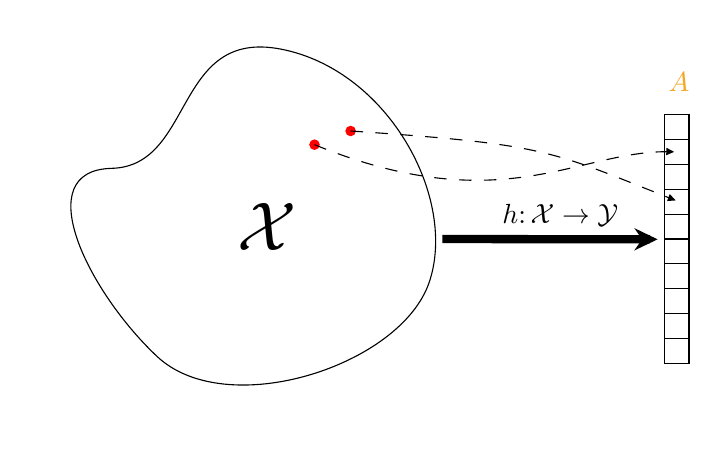
\begin{tikzpicture}[x=0.75pt,y=0.75pt,yscale=-0.6,xscale=0.6]
%uncomment if require: \path (0,300); %set diagram left start at 0, and has height of 300

%Shape: Regular Polygon [id:dp5892453846061058] 
\draw   (200.32,23.52) .. controls (286.72,40.31) and (342.31,143.62) .. (319.3,210.88) .. controls (296.28,278.15) and (156.47,322.59) .. (100.84,270.29) .. controls (45.2,217.99) and (-2.63,120.91) .. (64.25,119.25) .. controls (131.13,117.59) and (113.91,6.73) .. (200.32,23.52) -- cycle ;
%Straight Lines [id:da5940227274966229] 
\draw [line width=3]    (330,176) -- (496.75,176.24) ;
\draw [shift={(502.75,176.25)}, rotate = 180.08] [fill={rgb, 255:red, 0; green, 0; blue, 0 }  ][line width=0.08]  [draw opacity=0] (18.75,-9.01) -- (0,0) -- (18.75,9.01) -- (12.45,0) -- cycle    ;
%Shape: Grid [id:dp5884380060790032] 
\draw  [draw opacity=0] (508,76) -- (528,76) -- (528,276) -- (508,276) -- cycle ; \draw    ; \draw   (508,96) -- (528,96)(508,116) -- (528,116)(508,136) -- (528,136)(508,156) -- (528,156)(508,176) -- (528,176)(508,196) -- (528,196)(508,216) -- (528,216)(508,236) -- (528,236)(508,256) -- (528,256) ; \draw   (508,76) -- (528,76) -- (528,276) -- (508,276) -- cycle ;
%Shape: Circle [id:dp7080915007017408] 
\draw  [draw opacity=0][fill={rgb, 255:red, 255; green, 0; blue, 0 }  ,fill opacity=1 ] (252,89.25) .. controls (252,86.9) and (253.9,85) .. (256.25,85) .. controls (258.6,85) and (260.5,86.9) .. (260.5,89.25) .. controls (260.5,91.6) and (258.6,93.5) .. (256.25,93.5) .. controls (253.9,93.5) and (252,91.6) .. (252,89.25) -- cycle ;
%Curve Lines [id:da44474204475477297] 
\draw  [dash pattern={on 4.5pt off 4.5pt}]  (256.25,89.25) .. controls (415.95,100.2) and (415.01,104.7) .. (515.72,144.4) ;
\draw [shift={(517.25,145)}, rotate = 201.49] [fill={rgb, 255:red, 0; green, 0; blue, 0 }  ][line width=0.08]  [draw opacity=0] (6.25,-3) -- (0,0) -- (6.25,3) -- cycle    ;
%Shape: Circle [id:dp43426133236609155] 
\draw  [draw opacity=0][fill={rgb, 255:red, 255; green, 0; blue, 0 }  ,fill opacity=1 ] (223,100.25) .. controls (223,97.9) and (224.9,96) .. (227.25,96) .. controls (229.6,96) and (231.5,97.9) .. (231.5,100.25) .. controls (231.5,102.6) and (229.6,104.5) .. (227.25,104.5) .. controls (224.9,104.5) and (223,102.6) .. (223,100.25) -- cycle ;
%Curve Lines [id:da27933594579127596] 
\draw  [dash pattern={on 4.5pt off 4.5pt}]  (227.25,100.25) .. controls (379.22,162.13) and (439.54,103.94) .. (513.75,105.92) ;
\draw [shift={(516,106)}, rotate = 182.47] [fill={rgb, 255:red, 0; green, 0; blue, 0 }  ][line width=0.08]  [draw opacity=0] (6.25,-3) -- (0,0) -- (6.25,3) -- cycle    ;

% Text Node
\draw (163.5,145.4) node [anchor=north west][inner sep=0.75pt]  [font=\Huge]  {$\mathcal{X}$};
% Text Node
\draw (509.5,39.9) node [anchor=north west][inner sep=0.75pt]    {$\textcolor[rgb]{0.96,0.65,0.14}{\boldsymbol{A}}$};
% Text Node
\draw (376,145.9) node [anchor=north west][inner sep=0.75pt]    {$h\colon \mathcal{X}\rightarrow \mathcal{Y}$};



\end{tikzpicture}
\end{figure}
%%%%%%%%%%%%%%%%%%%%%%%%%%%%%%%%%%%%%%%%%%%%%%%%%%%%%%%%%%%%%%%%%%%%%%%%%%%
%%%%%%%%%%%%%%%%%%%%%%%%%%%%%%%%%%%%%%%%%%%%%%%%%%%%%%%%%%%%%%%%%%%%%%%%%%%



The sad truth is that collisions are inevitable, no matter how carefully we design our hash functions; and, even worse, we already saw why! This is the birthday paradox.
\begin{fact}
    Suppose $\orange{A}$ is of size $\green{m'} \leq c\cdot \ns^2$, for some absolute constant $c>0$. Then, even if the hash function $h\colon\cX\to [\green{m'}]$ was truly random, or even if the $\ns$ data points were truly independent uniformly random elements of $\cX$, there would still be a $99\%$ probability at least two elements of the data structure are hashed to the same bucket of $\orange{A}$.
\end{fact}
It is even worse than that: since we would like to take $\green{m'}=O(\ns)$, we also have this other result we saw earlier\dots\marginnote{At least, for this one, we have some idea of how we could try and resolve it: the power of two choices might help? Peeking ahead, this is the idea behind Cuckoo Hashing.}
\begin{fact}
    Suppose $\orange{A}$ is of size $\green{m'} \leq c\cdot \ns$, for some absolute constant $c>0$. Then, even if the hash function $h\colon\cX\to [\green{m'}]$ was truly random, or even if the $\ns$ data points were truly independent uniformly random elements of $\cX$, the expected maximum load among all buckets of $\orange{A}$ would be $\bigOmega{\frac{\log\ns}{\log\log\ns}}$. That is, we would expect at least one of the buckets to have at least this many hash collisions.
\end{fact}
%After all, in the array above, all but $\ns$ out of $\green{m}$ locations of the array are use
\subsection{Handling collisions}
Fortunately, there are many strategies to handle collisions, each with its advantages and drawbacks. We can divide them in two broad families: \emph{separate chaining}, and \emph{open addressing}.
\paragraph{(Separate) chaining}
Separate chaining is the most natural strategy: everybody hash value gets a list! If several of our $\ns$ data points are hashed to the same bucket in $\orange{A}$, add them to a linked list! That is, $\orange{A}[y]$ will link to a list of all the elements $x$ we want to store such that $h(x)=y$. To implement the 3 operations, we then just delegate to the list stored in the bucket:
    \begin{itemize}
        \item$\textsc{Insert}(x)$: call $\orange{A}[h(x)].\textsc{Insert}(x)$
        \item$\textsc{Lookup}(x)$: return $\orange{A}[h(x)].\textsc{Lookup}(x)$
        \item$\textsc{Remove}(x)$: call $\orange{A}[h(x)].\textsc{Remove}(x)$
    \end{itemize}
%%%%%%%%%%%%%%%%%%%%%%%%%%%%%%%%%%%%%%%%%%%%%%%%%%%%%%%%%%%%%%%%%%%%%%%%%%%
%%%%%%%%%%%%%%%%%%%%%%%%%%%%%%%%%%%%%%%%%%%%%%%%%%%%%%%%%%%%%%%%%%%%%%%%%%%
\begin{figure}
\tikzset{every picture/.style={line width=0.75pt}} %set default line width to 0.75pt     
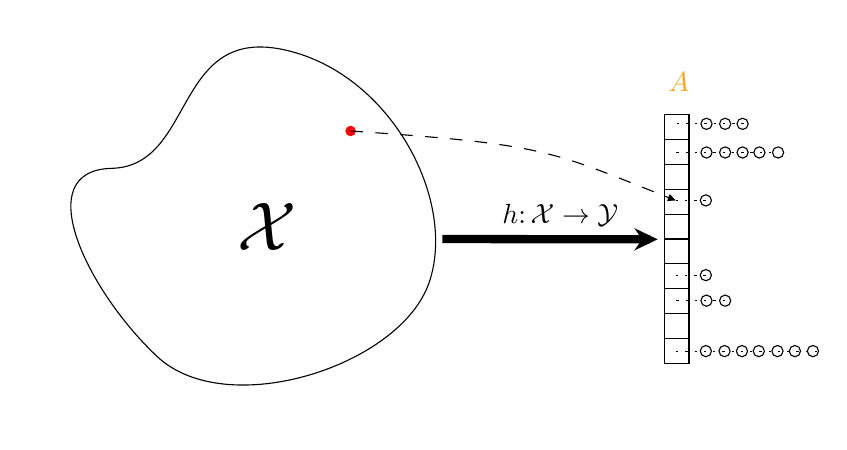
\begin{tikzpicture}[x=0.75pt,y=0.75pt,yscale=-0.6,xscale=0.6]
%uncomment if require: \path (0,300); %set diagram left start at 0, and has height of 300

%Shape: Regular Polygon [id:dp8090699692325243] 
\draw   (202.32,22.52) .. controls (288.72,39.31) and (344.31,142.62) .. (321.3,209.88) .. controls (298.28,277.15) and (158.47,321.59) .. (102.84,269.29) .. controls (47.2,216.99) and (-0.63,119.91) .. (66.25,118.25) .. controls (133.13,116.59) and (115.91,5.73) .. (202.32,22.52) -- cycle ;
%Straight Lines [id:da022629349356171446] 
\draw [line width=3]    (332,175) -- (498.75,175.24) ;
\draw [shift={(504.75,175.25)}, rotate = 180.08] [fill={rgb, 255:red, 0; green, 0; blue, 0 }  ][line width=0.08]  [draw opacity=0] (18.75,-9.01) -- (0,0) -- (18.75,9.01) -- (12.45,0) -- cycle    ;
%Shape: Grid [id:dp05145666164983498] 
\draw  [draw opacity=0] (510,75) -- (530,75) -- (530,275) -- (510,275) -- cycle ; \draw    ; \draw   (510,95) -- (530,95)(510,115) -- (530,115)(510,135) -- (530,135)(510,155) -- (530,155)(510,175) -- (530,175)(510,195) -- (530,195)(510,215) -- (530,215)(510,235) -- (530,235)(510,255) -- (530,255) ; \draw   (510,75) -- (530,75) -- (530,275) -- (510,275) -- cycle ;
%Shape: Circle [id:dp6479250592118756] 
\draw   (539.5,82.5) .. controls (539.5,80.01) and (541.51,78) .. (544,78) .. controls (546.49,78) and (548.5,80.01) .. (548.5,82.5) .. controls (548.5,84.99) and (546.49,87) .. (544,87) .. controls (541.51,87) and (539.5,84.99) .. (539.5,82.5) -- cycle ;
%Shape: Circle [id:dp34702826817417354] 
\draw   (554.5,82.5) .. controls (554.5,80.01) and (556.51,78) .. (559,78) .. controls (561.49,78) and (563.5,80.01) .. (563.5,82.5) .. controls (563.5,84.99) and (561.49,87) .. (559,87) .. controls (556.51,87) and (554.5,84.99) .. (554.5,82.5) -- cycle ;
%Shape: Circle [id:dp4536557388273843] 
\draw   (568.5,82.5) .. controls (568.5,80.01) and (570.51,78) .. (573,78) .. controls (575.49,78) and (577.5,80.01) .. (577.5,82.5) .. controls (577.5,84.99) and (575.49,87) .. (573,87) .. controls (570.51,87) and (568.5,84.99) .. (568.5,82.5) -- cycle ;
%Shape: Circle [id:dp8353479068292242] 
\draw   (539.5,105.5) .. controls (539.5,103.01) and (541.51,101) .. (544,101) .. controls (546.49,101) and (548.5,103.01) .. (548.5,105.5) .. controls (548.5,107.99) and (546.49,110) .. (544,110) .. controls (541.51,110) and (539.5,107.99) .. (539.5,105.5) -- cycle ;
%Shape: Circle [id:dp38555811039605437] 
\draw   (554.5,105.5) .. controls (554.5,103.01) and (556.51,101) .. (559,101) .. controls (561.49,101) and (563.5,103.01) .. (563.5,105.5) .. controls (563.5,107.99) and (561.49,110) .. (559,110) .. controls (556.51,110) and (554.5,107.99) .. (554.5,105.5) -- cycle ;
%Shape: Circle [id:dp7008873748312328] 
\draw   (568.5,105.5) .. controls (568.5,103.01) and (570.51,101) .. (573,101) .. controls (575.49,101) and (577.5,103.01) .. (577.5,105.5) .. controls (577.5,107.99) and (575.49,110) .. (573,110) .. controls (570.51,110) and (568.5,107.99) .. (568.5,105.5) -- cycle ;
%Shape: Circle [id:dp750804228542512] 
\draw   (582,105.5) .. controls (582,103.01) and (584.01,101) .. (586.5,101) .. controls (588.99,101) and (591,103.01) .. (591,105.5) .. controls (591,107.99) and (588.99,110) .. (586.5,110) .. controls (584.01,110) and (582,107.99) .. (582,105.5) -- cycle ;
%Shape: Circle [id:dp13100978706796573] 
\draw   (597,105.5) .. controls (597,103.01) and (599.01,101) .. (601.5,101) .. controls (603.99,101) and (606,103.01) .. (606,105.5) .. controls (606,107.99) and (603.99,110) .. (601.5,110) .. controls (599.01,110) and (597,107.99) .. (597,105.5) -- cycle ;
%Shape: Circle [id:dp9837665512770466] 
\draw   (539,144) .. controls (539,141.51) and (541.01,139.5) .. (543.5,139.5) .. controls (545.99,139.5) and (548,141.51) .. (548,144) .. controls (548,146.49) and (545.99,148.5) .. (543.5,148.5) .. controls (541.01,148.5) and (539,146.49) .. (539,144) -- cycle ;
%Shape: Circle [id:dp7642283303814478] 
\draw   (539,204) .. controls (539,201.51) and (541.01,199.5) .. (543.5,199.5) .. controls (545.99,199.5) and (548,201.51) .. (548,204) .. controls (548,206.49) and (545.99,208.5) .. (543.5,208.5) .. controls (541.01,208.5) and (539,206.49) .. (539,204) -- cycle ;
%Shape: Circle [id:dp6692954665359216] 
\draw   (539.5,224.5) .. controls (539.5,222.01) and (541.51,220) .. (544,220) .. controls (546.49,220) and (548.5,222.01) .. (548.5,224.5) .. controls (548.5,226.99) and (546.49,229) .. (544,229) .. controls (541.51,229) and (539.5,226.99) .. (539.5,224.5) -- cycle ;
%Shape: Circle [id:dp8910308062853909] 
\draw   (554.5,224.5) .. controls (554.5,222.01) and (556.51,220) .. (559,220) .. controls (561.49,220) and (563.5,222.01) .. (563.5,224.5) .. controls (563.5,226.99) and (561.49,229) .. (559,229) .. controls (556.51,229) and (554.5,226.99) .. (554.5,224.5) -- cycle ;
%Shape: Circle [id:dp21020217647833994] 
\draw   (539,265) .. controls (539,262.51) and (541.01,260.5) .. (543.5,260.5) .. controls (545.99,260.5) and (548,262.51) .. (548,265) .. controls (548,267.49) and (545.99,269.5) .. (543.5,269.5) .. controls (541.01,269.5) and (539,267.49) .. (539,265) -- cycle ;
%Shape: Circle [id:dp5092131007727523] 
\draw   (554,265) .. controls (554,262.51) and (556.01,260.5) .. (558.5,260.5) .. controls (560.99,260.5) and (563,262.51) .. (563,265) .. controls (563,267.49) and (560.99,269.5) .. (558.5,269.5) .. controls (556.01,269.5) and (554,267.49) .. (554,265) -- cycle ;
%Shape: Circle [id:dp6005647648405279] 
\draw   (568,265) .. controls (568,262.51) and (570.01,260.5) .. (572.5,260.5) .. controls (574.99,260.5) and (577,262.51) .. (577,265) .. controls (577,267.49) and (574.99,269.5) .. (572.5,269.5) .. controls (570.01,269.5) and (568,267.49) .. (568,265) -- cycle ;
%Shape: Circle [id:dp6056236374130685] 
\draw   (581.5,265) .. controls (581.5,262.51) and (583.51,260.5) .. (586,260.5) .. controls (588.49,260.5) and (590.5,262.51) .. (590.5,265) .. controls (590.5,267.49) and (588.49,269.5) .. (586,269.5) .. controls (583.51,269.5) and (581.5,267.49) .. (581.5,265) -- cycle ;
%Shape: Circle [id:dp6814289868642057] 
\draw   (596.5,265) .. controls (596.5,262.51) and (598.51,260.5) .. (601,260.5) .. controls (603.49,260.5) and (605.5,262.51) .. (605.5,265) .. controls (605.5,267.49) and (603.49,269.5) .. (601,269.5) .. controls (598.51,269.5) and (596.5,267.49) .. (596.5,265) -- cycle ;
%Shape: Circle [id:dp4003339160068812] 
\draw   (610.5,265) .. controls (610.5,262.51) and (612.51,260.5) .. (615,260.5) .. controls (617.49,260.5) and (619.5,262.51) .. (619.5,265) .. controls (619.5,267.49) and (617.49,269.5) .. (615,269.5) .. controls (612.51,269.5) and (610.5,267.49) .. (610.5,265) -- cycle ;
%Shape: Circle [id:dp5195042865870344] 
\draw   (625,265) .. controls (625,262.51) and (627.01,260.5) .. (629.5,260.5) .. controls (631.99,260.5) and (634,262.51) .. (634,265) .. controls (634,267.49) and (631.99,269.5) .. (629.5,269.5) .. controls (627.01,269.5) and (625,267.49) .. (625,265) -- cycle ;
%Straight Lines [id:da10849130917681804] 
\draw  [dash pattern={on 0.84pt off 2.51pt}]  (520,82.5) -- (577.5,82.5) ;
%Straight Lines [id:da8301322053157919] 
\draw  [dash pattern={on 0.84pt off 2.51pt}]  (519.75,105.5) -- (601.5,105.5) ;
%Straight Lines [id:da6070616319798346] 
\draw  [dash pattern={on 0.84pt off 2.51pt}]  (519.25,144) -- (543.5,144) ;
%Straight Lines [id:da9016627948586332] 
\draw  [dash pattern={on 0.84pt off 2.51pt}]  (519.75,224.5) -- (563.5,224.5) ;
%Straight Lines [id:da5771080093661222] 
\draw  [dash pattern={on 0.84pt off 2.51pt}]  (519.5,265) -- (634,265) ;
%Straight Lines [id:da7159109321410426] 
\draw  [dash pattern={on 0.84pt off 2.51pt}]  (519.25,204) -- (543.5,204) ;
%Shape: Circle [id:dp8642716773725309] 
\draw  [draw opacity=0][fill={rgb, 255:red, 255; green, 0; blue, 0 }  ,fill opacity=1 ] (254,88.25) .. controls (254,85.9) and (255.9,84) .. (258.25,84) .. controls (260.6,84) and (262.5,85.9) .. (262.5,88.25) .. controls (262.5,90.6) and (260.6,92.5) .. (258.25,92.5) .. controls (255.9,92.5) and (254,90.6) .. (254,88.25) -- cycle ;
%Curve Lines [id:da3950336012128167] 
\draw  [dash pattern={on 4.5pt off 4.5pt}]  (258.25,88.25) .. controls (417.95,99.2) and (417.01,103.7) .. (517.72,143.4) ;
\draw [shift={(519.25,144)}, rotate = 201.49] [fill={rgb, 255:red, 0; green, 0; blue, 0 }  ][line width=0.08]  [draw opacity=0] (6.25,-3) -- (0,0) -- (6.25,3) -- cycle    ;

% Text Node
\draw (165.5,144.4) node [anchor=north west][inner sep=0.75pt]  [font=\Huge]  {$\mathcal{X}$};
% Text Node
\draw (511.5,38.9) node [anchor=north west][inner sep=0.75pt]    {$\textcolor[rgb]{0.96,0.65,0.14}{\boldsymbol{A}}$};
% Text Node
\draw (378,144.9) node [anchor=north west][inner sep=0.75pt]    {$h\colon \mathcal{X}\rightarrow \mathcal{Y}$};
\end{tikzpicture}
\end{figure}
%%%%%%%%%%%%%%%%%%%%%%%%%%%%%%%%%%%%%%%%%%%%%%%%%%%%%%%%%%%%%%%%%%%%%%%%%%%
%%%%%%%%%%%%%%%%%%%%%%%%%%%%%%%%%%%%%%%%%%%%%%%%%%%%%%%%%%%%%%%%%%%%%%%%%%%
In that sense, it combines the hash table (which is based on the naive array-based approach) with the linked-list approach, in an attempt to get the best of both worlds. 
Let
\begin{equation}
    \label{def:load:hashtable}
\alpha = \frac{\ns}{\green{m'}}
\end{equation}
denote the \emph{load factor} of the hash table. For $\green{m'} = O(\ns)$, this will be a (small) constant. Then:\marginnote{Note that chaining allows the load $\alpha$ to be greater than $1$. The next strategy, open addressing, does not.}
\begin{itemize}
    \item the total space used will be 
    \[
    O(\log\green{m} + \green{m'} + \ns \log \green{m}) = O((1+\alpha)\green{m'} \log \green{m})
    \]
    (the cost of storing the hash function, and the total space used by the array itself and by all the lists: that last one is proportional to the numbers $\ns$ of elements currently stored).
    \item by linearity of expectation, the \emph{expected} time complexity of all 3 operations is $O(1+\alpha)$, since $\alpha$ is the expected size of any given list.
    \item \dots but (think of the max load argument), most likely than not we will have some of the buckets for which the list has size $\Omega(\log\ns/\log\log\ns)$.\marginnote{This leads, for those, to a performance comparable to that of the BST approach!} 
\end{itemize}

\marginnote{\TODO{} {Give more detail here? Empirical evaluation of the maximum load for the family of hash functions given above.}}
\paragraph{Open addressing}
Another approach to handle collisions is \emph{open addressing}, which itself comes in several variants. The basic idea is quite simple: instead of a single hash function, we have a sequence of hash functions $h_1,\dots,h_t,\dots, h_{\green{m'}}$. If we are trying to insert an element $x$ in the hash table, we look at the bucket $h_1(x)$: if it's already taken (collision!), then we go to $h_1(x)$: if taken, we look at $h_3(x)$; etc. We stop when we found an empty bucket.\footnote{If there is no empty bucket, then this means the hash table is full (the load factor is $\alpha=1$) and we need to increase $\green{m'}$ to resize $\orange{A}$~--~an expensive operation, as this means re-hashing all elements.}

That is, we have the following:
    \begin{itemize}
        \item$\textsc{Insert}(x)$: 
            \begin{algorithmic}
                \ForAll{$1\leq t\leq \green{m'}$}
                    \If{$\orange{A}[h_t(x)]=x$}
                        \State \Return \Comment{Already there}
                    \ElsIf{$\orange{A}[h_t(x)]=\emptyset$ or $\orange{A}[h_t(x)]=\bot$}
                        \State $\orange{A}[h_t(x)]\gets x$ \Comment{Insert it in the first available bucket}
                        \State \Return 
                    \EndIf
                \EndFor
            \end{algorithmic}
        \item$\textsc{Lookup}(x)$: 
            \begin{algorithmic}
                \ForAll{$1\leq t\leq \green{m'}$}
                    \If{$\orange{A}[h_t(x)]=x$}
                        \State \Return \yes
                    \ElsIf{$\orange{A}[h_t(x)]=\emptyset$}
                        \State \Return \no \Comment{If $x$ was present, it'd have been found earlier}
                    \EndIf
                \EndFor
            \end{algorithmic}
        \item$\textsc{Remove}(x)$: 
                    \begin{algorithmic}
                \ForAll{$1\leq t\leq \green{m'}$}
                    \If{$\orange{A}[h_t(x)]=x$}
                        \State $\orange{A}[h_t(x)]\gets \bot$ \Comment{Special symbol to indicate there was something before}
                        \State \Return
                    \ElsIf{$\orange{A}[h_t(x)]=\emptyset$}
                        \State \Return \Comment{If $x$ was present, it'd have been found earlier}
                    \EndIf
                \EndFor
            \end{algorithmic}
    \end{itemize}
You may wonder why we have this strange symbol $\bot$ when we remove an element $x$. The reason is that if we just emptied that bucket by (making it $\emptyset$), this would potentially mess up future lookups: we would not know when to stop searching! \medskip

But \emph{how do we choose this sequence of hash functions?} We would like a few things: first, to make sure we cover all possible buckets: namely, for every $x\in\cX$, we want
\[
(h_1(x),\dots, h_{\green{m'}}(x))
\]
to me a permutation of $\{0,1,2,\dots,\green{m'}\}$. This is to make sure we do explore all possible buckets when trying to lookup or insert an element, if we keep finding collisions. Second, we would like to be able to \emph{store} (and evaluate) them all succinctly. We had only one hash function before, and we went to great lengths to make sure it did not take too much space to store, only $O(\log \green{m})$ bits: now, if we have $\green{m'}$, we'd like to avoid blowing up our space usage by that factor! For $\green{m'}=O(\ns)$, that would use space $O(\ns \log \green{m})$\dots

Before discussing (briefly) some common choices for this sequence of hash functions, let us first analyze the resulting (expected) time complexities of our 3 methods, under some very idealized (and unrealistic) assumptions:
\begin{theorem}
    \label{theo:wsishful:addressing}
    Assume that our sequence of hash functions is such that, for every element $x\in\cX$, the (random) sequence $(h_1(x),\dots, h_{\green{m'}}(x))$ is a uniformly random permutation of $[\green{m'}]$. Then, for every $x\in\cX$, \textsc{Lookup} runs in expected time 
    \[
    \bigO{\frac{1}{1-\alpha}}
    \]
   where $\alpha$ is the \emph{load factor} of the hash table, as defined in~\eqref{def:load:hashtable}.
\end{theorem}
\begin{proof}
    Fix any $x\in\cX$. Since we want to upper bound the expected running time, it is enough to consider the case where $x$ is \emph{not} in the data structure (unsuccessful lookup), since otherwise the search will end earlier (once it finds $x$). So the time here will be the number of steps until an empty bucket is found (in which case $\textsc{Lookup}$ finally will return $\no$).
    
    By symmetry, the probability that any given bucket is empty is equal to $1-\frac{\ns}{\green{m'}}$. Let $T(\ns, \green{m'})$ be the time taken by an (unsuccessful) search for item $x$ in the hash table of size $\green{m'}$ containing $\ns$ hash values. If the first index checked corresponds to an empty bucket (with by the above happens with probability $\frac{\ns}{\green{m'}}$), then the search ends after this one step; otherwise, we continue on the remaining subarray of $\green{m'}-1$ buckets, containing the remaining $\ns-1$ hash values. And, crucially, the remaining sequence of hash functions values $(h_2(x),\dots, h_{\green{m'}}(x))$ is \emph{still} a uniformly random permutation of these remaining $\green{m'}-1$ buckets (all except the bucket $h_1(x)$, which has been looked at already). 
    So we have the recurrence relation:
    \[
        \bEE{T(\ns, \green{m'})} = 1 + \frac{\ns}{\green{m'}}\cdot  \bEE{T(\ns-1, \green{m'}-1)}
    \]
    We can then prove by induction (over $\ns$) that the solution is 
    \[
    \bEE{T(\ns, \green{m'})} \leq \frac{1}{1-\frac{\ns}{\green{m'}}}\,,
    \]
    which concludes the proof.
\end{proof}
With this in hand, here are some of the common strategies to implement open addressing:
\begin{itemize}
    \item Linear probing: forget about using completely distinct hash functions! We have \emph{one} hash function $h$, let us make the most out of it and just look at the next bucket at each step:
    \[
        h_t(x) = h(x)+(t-1) \bmod \green{m'}
    \]
    On the plus side, this is very good in terms of space complexity (we still only store \emph{one} hash function), and very fast to evaluate (as long as $h$ itself is fast to evaluate). How well does this do? The time complexity of any of the 3 functions is again related to the {load factor} of the hash table, and quickly degrades as $\alpha$ gets close to $1$. Namely, we have:
    \begin{theorem}[Knuth'62]
        Assume for simplicity that the hash function $h\colon \cX\to\cY$ is a truly random function, and furthermore that the loads of each bucket , $(|h^{-1}(y)|)_{y\in[\green{m'}}$, are independent. Then, the expected time complexities of \textsc{Insert}, \textsc{Lookup}, and \textsc{Remove} are all $\bigO{\frac{1}{(1-\alpha)^2}}$.
    \end{theorem}
    We will not prove this here, but this is actually quite surprising (and bad), and shows that linear probing actually performs much worse than one would think! Indeed, compare this to the wishful analysis of~\cref{theo:wsishful:addressing}.
    \item Quadratic probing: the same idea, but now
    \[
        h_t(x) = h(x)+c_1 t + c_2 t^2 \bmod \green{m'}
    \]
    for two constants $c_1,c_2$ with $c_2 \neq 0$ chosen somewhat arbitrarily (but in order to get a permutation of $\{0,1,2,\dots,\green{m'}\}$). This is supposed to incur less ``clustering'' of values than linear probing, while having the same advantages.
    \item Double hashing: we use \emph{two} hash functions, $h,g$, and set
        \[
        h_t(x) = h(x)+(t-1)\cdot g(x) \bmod \green{m'}
        \]
    \item Cuckoo hashing: this one is really neat, as it goes beyond \emph{expected} running times, and actually provides \emph{worst-case} running time guarantees for 2 out of 3 operations. This hashing strategy was proposed and analyzed by Pagh and Flemming in 2001,\cite{PaghR01,PaghR04} and relies on a beautiful idea you have seen in an earlier lecture: the power of two choices. Specifically, the data structure uses two hash tables, $h_1, \orange{A_1}$ and  $h_2, \orange{A_2}$. An element $x\in \cX$ can only be hashed to one of its two locations, either $\orange{A_1}[h_1(x)]$ or $\orange{A_2}[h_2(x)]$: so for lookups and removals, it suffices to check both of these.

        \begin{itemize}
        \item$\textsc{Lookup}(x)$: 
            \begin{algorithmic}
                \If{$\orange{A_1}[h_1(x)]=x$ or $\orange{A_2}[h_2(x)]=x$}
                        \State \Return \yes
                    \Else
                        \State \Return \no
                    \EndIf
            \end{algorithmic}
        \item$\textsc{Remove}(x)$: 
                    \begin{algorithmic}
                \If{$\orange{A_1}[h_1(x)]=x$}
                        \State $\orange{A_1}[h_1(x)] \gets \emptyset$
                \ElsIf{$\orange{A_2}[h_2(x)]=x$}
                        \State $\orange{A_2}[h_2(x)] \gets \emptyset$
                \EndIf
            \end{algorithmic}
    \end{itemize}

    For insertions, it is a bit more complicated. When inserting an element $x$, if either $\orange{A_1}[h_1(x)]$ or $\orange{A_2}[h_2(x)]$ is empty, we are done: we can insert $x$ to that empty slot. If both are currently occupied, say by two other elements $x'$ and $x''$\dots then, an \emph{eviction} occurs (which is where the ``cuckoo'' part of the name comes from. Cuckoos are\dots not very nice birds.). That is, $x$ takes the spot of $x'$, forcing $x'$ to go to its own other location in $\orange{A_2}$. If that location is empty, then $x'$ goes there and everyone is happy: but if \emph{another} element was there\dots then $x'$ takes that spot, forcing that element itself to go to its alternate location in the other hash table. And so on and so forth, until the cycle ends or the maximum number of evictions has been reached.
    \begin{itemize}
        \item$\textsc{Insert}(x)$: 
                    \begin{algorithmic}
                \If{$\orange{A_1}[h_1(x)]=\emptyset$}
                        \State $\orange{A_1}[h_1(x)] \gets x$
                \ElsIf{$\orange{A_2}[h_2(x)]=\emptyset$}
                        \State $\orange{A_2}[h_2(x)] \gets x$
                \Else
                    \State $T \gets 0$ \Comment{The evictions start}
                    \State $x' \gets \orange{A_1}[h_1(x)]$
                    \State $\orange{A_1}[h_1(x)] \gets x$
                    \While{$T < T_{\max}$}
                    \State $x'$ goes to $\orange{A_2}[h_2(x')]$, and if there was something there, that element now needs to move, etc.
                    \State $T\gets T+1$
                    \EndWhile                    
                \EndIf
            \end{algorithmic}
    \end{itemize}
    \begin{theorem}
        Cuckoo hashing achieves worst-case time $O(1)$ for \textsc{Lookup} and
\textsc{Remove}, and expected time $O(1)$ for \textsc{Insert}.
    \end{theorem}
    The guarantees for \textsc{Lookup} and \textsc{Remove} are immediate; the expected guarantee for \textsc{Insert}, however, is quite involved. We will not prove it here (but will discuss some of it during the tutorial).
\end{itemize}

\begin{remark}[And there is more!]
There are other strategies, such as 2-level hashing (where we use a second hash table for each bucket). We will see more during the tutorial.
\end{remark}
%\subsection{Applications}
%2-sum?
% Talk about "why do things appear to work so well" -- the Mitzenmacher--Vadhan paper? http://timroughgarden.org/f14/l/l16_old.pdf
%%%%%%%%%%%%%%%%%%%%%%%%%%%%%%%%%%%%%%%%
\subsection{Bloom filters}

As we saw above, a hash table allows us to store and retrieve data very quickly (in expectation, or ``for typical data''); the data structures never ``make mistakes'', since the result is always correct, and the only random aspect is the time complexity. But while they are typically faster and very space efficient, hash tables do still use some \emph{space}: if each element $x\in \cX$ takes $\log_2 \green{m}$ (where $\green{m} = |\cX|$) bits to store, a hash table will take $O(\ns\log \green{m})$ space to store $\ns$ elements. Which is very little, and usually alright, but \emph{sometimes} is not.
	
	In this short section, we will see a related data structure, the \emph{Bloom filter}, which uses much less space while still providing efficient access and insertion: only $O(\ns)$ space to store $\ns$ elements (regardless of how many bits an element takes to encode)! But this comes at a price: sometimes, the result of a query to the data structure will be wrong. However, when designed well, the frequency with which those mistakes occur is relatively low, and can be controlled.
	
	Let us start with what a Bloom filter is. For simplicity, here we will only allow insertions ($\textsc{Insert}$) and lookups ($\textsc{Lookup}$), but no deletions.\footnote{They could be implemented, but this adds quite a bit of complexity to the data structure.} The Bloom filter is an array $\orange{A}$ of size $\green{m'}$ (containing $\green{m'}$ bits, initialized to $0$), along with $\blue{k}$ distinct hash functions $h_1,\dots,h_{\blue{k}}$, each mapping the data universe $\cX$ to $[\green{m'}] = \{1,2,\dots,\green{m'}\}$:
	\[
		h_i\colon \cX \to \cY = [\green{m'}], \qquad i\in\{1,2,\dots,m\}
	\]
	where $\green{m'}$ and $\blue{k}$ are parameters to choose. Here is how it works: given an element $x\in \cX$,
	\begin{itemize}
	\item $\textsc{insert}(x)$ evaluates the $\blue{k}$ hash functions on $x$ and sets the bit of all $\blue{k}$ corresponding cells to $1$.
		\begin{algorithmic}
		  \Function{Insert}{$x$}
		  \ForAll{$1\leq i \leq \blue{k}$}
			  \State $\orange{A}[h_i(x)] \gets 1$
		  \EndFor
		  \EndFunction
		\end{algorithmic}
	\item $\textsc{Lookup}(x)$ evaluates the $\blue{k}$ hash functions on $x$ and checks that all the $\blue{k}$ bits in the corresponding cells are equal to $1$.
		\begin{algorithmic}
		  \Function{Lookup}{$x$}
		  \ForAll{$1\leq i \leq \blue{k}$}
			  \If{ $\orange{A}[h_i(x)] = 0$ }
			  	\State \Return \no
			  \EndIf
		  \EndFor
		  \State \Return \yes
		  \EndFunction
		\end{algorithmic}
	\end{itemize}'

 That's all! In the rest of this lecture, we will try to see what this does, how to analyze the performance, and see how to choose the parameter $\blue{k}$ (number of hash functions).

 \paragraph{What type of ``mistakes'' can $\textsc{Lookup}$ make?}

 A Bloom filter can only make one type of errors:  \emph{false positives} (returning \yes when the element is not in the data structure), never any \emph{false negative} (returning \no although the element \emph{is} in the data structure). This is because once its corresponding bits are set to $1$, the element will always be reported as present. But a non-present element might have its $\blue{k}$ bits set to $1$ by several other elements. Here's an example with $m=3$, $N=10$, and $\cX=\{1,2,3,4\}$: consider the hash functions
\begin{center}
\begin{tabular}{|c|c|c|c|}\hline
	& $h_1$ & $h_2$& $h_3$ \\\hline
	1&1&5&10\\\hline
	2&9&4&6\\\hline
	3&1&6&3 \\\hline
	4&7&3&8\\\hline
\end{tabular}
\end{center}
~\newline

Say we insert $S=\{1,2,4\}$: the corresponding bits set to $1$ will be (indexing starting at $1$)
\begin{align*}
	1 &\leadsto \orange{A}[1], \orange{A}[5], \orange{A}[10] \\
	2 &\leadsto \orange{A}[9], \orange{A}[4], \orange{A}[6] \\
	4 &\leadsto \orange{A}[7], \orange{A}[3], \orange{A}[8]
\end{align*}

Now, when calling $\textsc{Lookup}(3)$, we will check if the bits $\orange{A}[1], \orange{A}[6], \orange{A}[3]$ are all equal to $1$. And they all are, so $\textsc{Lookup}(3)$ will return \yes even though $3$ was \emph{not} inserted.

\paragraph{Space complexity}
Assuming each hash function can be stored in $O(\log\green{m})$ space and takes $O(1)$ time to evaluate, the space complexity of the Bloom filter is
\begin{equation}
    \label{eq:bloomfiler:space}
    O(\blue{k}\log\green{m} + \green{m'})
\end{equation}
and the (worst-case) time complexities of $\textsc{Insert}$ and $\textsc{Lookup}$ are $O(\blue{k})$.

\paragraph{Error probability}
Under the idealized (that is: wrong) simplifying assumption that all $\blue{k}$ hash functions behave like independent, truly random functions, one can show that the probability that $\textsc{Lookup}$ makes an error after $\ns$ elements have been inserted in the data structure is
\begin{equation}
\label{eq:bloomfiler:error}
\Paren{1-\Paren{1-\frac{1}{\green{m'}}^{\ns \blue{k}}}}^{\blue{k}} \approx 
\Paren{1-e^{-\frac{\ns \blue{k}}{\green{m'}}}}^{\blue{k}}
\end{equation}
By looking at the tradeoff between space \eqref{eq:bloomfiler:space} and error probability \eqref{eq:bloomfiler:error}, one can then set the parameters $\blue{k}$ and $\green{m'}$ as desired. For instance, for a fixed $\ns$ and a target value of space $\green{m'}$, we can derive the optimal value of $\blue{k}$ to set in order to minimize the probability of error.

\chapter{Lecture 7: Nearest Neighbours and dimensionality reduction}
Last week, we focused on hash tables and Bloom filters, which enable us to solve the \emph{dictionary problem}:
\begin{framed}
    Given a dataset $S$, subset of a very large ``universe'' $\cX$, how do we quickly check if a new element $x\in\cX$ is in the dataset?
\end{framed}
This week, we will focus on a different, but related question, which can be seen as a ``relaxed'' version of the dictionary problem. Namely, we will not ask whether a query $x$ is \emph{in} the dataset, but instead we will ask to return a point $y\in S$ that is \emph{close} to $x$~--~ideally, the closest. You can see the applications of this question: (1)~given a noisy version $x$ of an image, find the closest picture stored in the dataset (i.e., a ``denoised'' version of $x$); (2)~given a point in a high-dimensional space, cluster it by finding a close center; (3)~given an assignment submitted this semester, find the most similar in the database of assignments from previous years\dots{} those are only a few examples. 

To even start, we need to define what ``close'' means: that is, we need a notion of \emph{distance} between elements of the universe $\cX$. This can be weakened a little, but here we will assume $\cX$ is a metric space, and comes with a metric\footnote{That is, $\dist{}{}$ is non-negative,
reflexive:
\[
\dist{x}{y} = 0 \Leftrightarrow x=y
\]
symmetric:
\[
\dist{x}{y} = \dist{y}{x},
\]
and satisfies the triangle inequality:
\[
\dist{x}{y} \leq \dist{x}{z}+\dist{z}{y}
\]
for all $x,y,z\in\cX$.
}
\[
\operatorname{dist}\colon \cX\times\cX \to \R_+\,.
\]
To give an example, think of a few metrics you most likely know or have encountered before:
\begin{enumerate}
    \item The \emph{Manhattan distance} on $\cX=\R^\dims$ (a.k.a. the $\lp[1]$ distance, or taxicab distance): $\dist{x}{y} = \sum_{i=1}^\dims \abs{x_i-y_i} = \normone{x-y}$
    \item The \emph{Euclidean distance} on $\cX=\R^\dims$ (a.k.a. the $\lp[2]$ distance): $\dist{x}{y} = \sqrt{\sum_{i=1}^\dims (x_i-y_i)^2} = \normtwo{x-y}$
    \item The \emph{Hamming distance} on $\cX=\bool^\dims$: $\dist{x}{y} = \sum_{i=1}^\dims \indicSet{x_i \neq y_i}$
\end{enumerate}
Any meaningful others?

With this in hand, we can define the problem we want to solve, the \emph{Nearest Neighbour Problem:}\marginnote{Nearest Neighbour (NN)}
\begin{framed}
    Given a dataset $S$, subset of a very large metric space $(\cX,\operatorname{dist})$, how to, given a new element $x\in\cX$, output an element $y\in S$ that minimises $\dist{x}{y}$?
\end{framed}
As before, we will let $\ns=|S|$ denote the current size of the dataset (which can change as we insert or remove elements), but instead of denoting by $\green{m}$ the size of the universe $\cX$, we will instead focus on high-dimensional universes such as $\bool^\dims$ or $\R^\dims$, and denote by $\dims$ the \emph{dimension} of the universe.\marginnote{So, for $\cX = \bool^\dims$, we have $\green{m}=2^\dims$. But for $\cX=\R^\dims$, $\green{m}=\infty$.}

%%%%%%%%%%%%%%%%%%%%%%%%%%%%%%%%%%%%%%%%%%%%%%%%%%%%%%%%%%%%%%%%%%%%%%%%%%
\begin{figure}\centering


\tikzset{every picture/.style={line width=0.75pt}} %set default line width to 0.75pt        

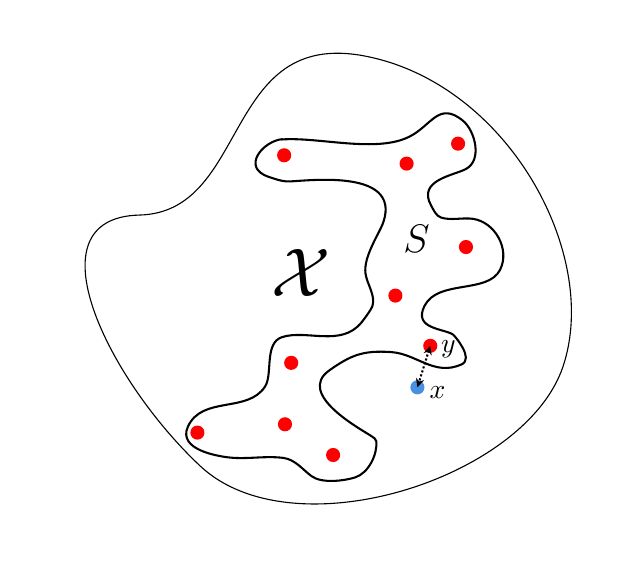
\begin{tikzpicture}[x=0.75pt,y=0.75pt,yscale=-0.8,xscale=0.8]
%uncomment if require: \path (0,300); %set diagram left start at 0, and has height of 300

%Shape: Regular Polygon [id:dp1730294945835068] 
\draw   (182.32,15.52) .. controls (268.72,32.31) and (324.31,135.62) .. (301.3,202.88) .. controls (278.28,270.15) and (138.47,314.59) .. (82.84,262.29) .. controls (27.2,209.99) and (-20.63,112.91) .. (46.25,111.25) .. controls (113.13,109.59) and (95.91,-1.27) .. (182.32,15.52) -- cycle ;
%Shape: Circle [id:dp299435924550042] 
\draw  [draw opacity=0][fill={rgb, 255:red, 255; green, 0; blue, 0 }  ,fill opacity=1 ] (196.25,159.75) .. controls (196.25,157.4) and (198.15,155.5) .. (200.5,155.5) .. controls (202.85,155.5) and (204.75,157.4) .. (204.75,159.75) .. controls (204.75,162.1) and (202.85,164) .. (200.5,164) .. controls (198.15,164) and (196.25,162.1) .. (196.25,159.75) -- cycle ;
%Shape: Circle [id:dp10120548228152837] 
\draw  [draw opacity=0][fill={rgb, 255:red, 255; green, 0; blue, 0 }  ,fill opacity=1 ] (234,68.25) .. controls (234,65.9) and (235.9,64) .. (238.25,64) .. controls (240.6,64) and (242.5,65.9) .. (242.5,68.25) .. controls (242.5,70.6) and (240.6,72.5) .. (238.25,72.5) .. controls (235.9,72.5) and (234,70.6) .. (234,68.25) -- cycle ;
%Shape: Circle [id:dp39541171931238484] 
\draw  [draw opacity=0][fill={rgb, 255:red, 255; green, 0; blue, 0 }  ,fill opacity=1 ] (203,80.25) .. controls (203,77.9) and (204.9,76) .. (207.25,76) .. controls (209.6,76) and (211.5,77.9) .. (211.5,80.25) .. controls (211.5,82.6) and (209.6,84.5) .. (207.25,84.5) .. controls (204.9,84.5) and (203,82.6) .. (203,80.25) -- cycle ;
%Shape: Circle [id:dp27264118237789015] 
\draw  [draw opacity=0][fill={rgb, 255:red, 255; green, 0; blue, 0 }  ,fill opacity=1 ] (217.25,190) .. controls (217.25,187.65) and (219.15,185.75) .. (221.5,185.75) .. controls (223.85,185.75) and (225.75,187.65) .. (225.75,190) .. controls (225.75,192.35) and (223.85,194.25) .. (221.5,194.25) .. controls (219.15,194.25) and (217.25,192.35) .. (217.25,190) -- cycle ;
%Shape: Circle [id:dp045119036480104846] 
\draw  [draw opacity=0][fill={rgb, 255:red, 255; green, 0; blue, 0 }  ,fill opacity=1 ] (77,242.25) .. controls (77,239.9) and (78.9,238) .. (81.25,238) .. controls (83.6,238) and (85.5,239.9) .. (85.5,242.25) .. controls (85.5,244.6) and (83.6,246.5) .. (81.25,246.5) .. controls (78.9,246.5) and (77,244.6) .. (77,242.25) -- cycle ;
%Shape: Circle [id:dp3583415724964084] 
\draw  [draw opacity=0][fill={rgb, 255:red, 255; green, 0; blue, 0 }  ,fill opacity=1 ] (158.75,255.75) .. controls (158.75,253.4) and (160.65,251.5) .. (163,251.5) .. controls (165.35,251.5) and (167.25,253.4) .. (167.25,255.75) .. controls (167.25,258.1) and (165.35,260) .. (163,260) .. controls (160.65,260) and (158.75,258.1) .. (158.75,255.75) -- cycle ;
%Shape: Circle [id:dp15906047769438314] 
\draw  [draw opacity=0][fill={rgb, 255:red, 255; green, 0; blue, 0 }  ,fill opacity=1 ] (133.5,200.25) .. controls (133.5,197.9) and (135.4,196) .. (137.75,196) .. controls (140.1,196) and (142,197.9) .. (142,200.25) .. controls (142,202.6) and (140.1,204.5) .. (137.75,204.5) .. controls (135.4,204.5) and (133.5,202.6) .. (133.5,200.25) -- cycle ;
%Shape: Circle [id:dp8324931679193618] 
\draw  [draw opacity=0][fill={rgb, 255:red, 255; green, 0; blue, 0 }  ,fill opacity=1 ] (129.25,75.25) .. controls (129.25,72.9) and (131.15,71) .. (133.5,71) .. controls (135.85,71) and (137.75,72.9) .. (137.75,75.25) .. controls (137.75,77.6) and (135.85,79.5) .. (133.5,79.5) .. controls (131.15,79.5) and (129.25,77.6) .. (129.25,75.25) -- cycle ;
%Shape: Circle [id:dp9687456268592909] 
\draw  [draw opacity=0][fill={rgb, 255:red, 74; green, 144; blue, 226 }  ,fill opacity=1 ] (209.5,215) .. controls (209.5,212.65) and (211.4,210.75) .. (213.75,210.75) .. controls (216.1,210.75) and (218,212.65) .. (218,215) .. controls (218,217.35) and (216.1,219.25) .. (213.75,219.25) .. controls (211.4,219.25) and (209.5,217.35) .. (209.5,215) -- cycle ;
%Shape: Circle [id:dp5806999822076053] 
\draw  [draw opacity=0][fill={rgb, 255:red, 255; green, 0; blue, 0 }  ,fill opacity=1 ] (238.75,130.5) .. controls (238.75,128.15) and (240.65,126.25) .. (243,126.25) .. controls (245.35,126.25) and (247.25,128.15) .. (247.25,130.5) .. controls (247.25,132.85) and (245.35,134.75) .. (243,134.75) .. controls (240.65,134.75) and (238.75,132.85) .. (238.75,130.5) -- cycle ;
%Shape: Free Drawing [id:dp0016405510888782837] 
\draw  [line width=0.75] [line join = round][line cap = round] (132.5,65.5) .. controls (120.64,66.63) and (107.3,82.71) .. (124.25,88.25) .. controls (127.77,89.4) and (131.31,90.77) .. (135,91) .. controls (142.47,91.46) and (204.55,81.59) .. (193.25,115.5) .. controls (191.11,121.93) and (181.01,136.28) .. (182.5,146.5) .. controls (183.45,153) and (188.5,159.42) .. (186.75,165.75) .. controls (186.04,168.31) and (180.74,175.09) .. (180,176) .. controls (167.78,190.94) and (146.96,180) .. (132.25,184.75) .. controls (121.35,188.27) and (126.79,207.08) .. (122,214.5) .. controls (111.51,230.75) and (84.05,219.84) .. (75.5,238.75) .. controls (69.18,252.74) and (94.12,256.55) .. (100.5,257.25) .. controls (111.27,258.42) and (122.25,256.12) .. (133,257.5) .. controls (140.19,258.43) and (144.71,264.63) .. (150,268.5) .. controls (156.26,273.08) and (169.72,271.29) .. (176.25,269.25) .. controls (184.31,266.73) and (189.79,255.28) .. (189,247.5) .. controls (188.86,246.15) and (187.37,245.27) .. (186.25,244.5) .. controls (180.98,240.88) and (140.1,219.28) .. (160.75,204.75) .. controls (173.61,195.7) and (180.68,192.66) .. (197.75,193.75) .. controls (213.53,194.76) and (223.66,208.48) .. (240.25,201.25) .. controls (248.2,197.78) and (236.02,183.77) .. (235.25,183.25) .. controls (229.68,179.5) and (211.02,179.96) .. (218,166) .. controls (226.06,149.87) and (256.01,158.93) .. (263.5,144.25) .. controls (269.77,131.96) and (260.54,115.32) .. (247,113.5) .. controls (240.72,112.65) and (234.04,114.68) .. (228,112.75) .. controls (225.01,111.79) and (223.52,108.24) .. (222,105.5) .. controls (213.51,90.21) and (235.59,87.42) .. (243,83.5) .. controls (253.03,78.2) and (248.46,60.44) .. (241.25,54.5) .. controls (226.63,42.46) and (222.34,57.27) .. (209,64) .. controls (188.84,74.17) and (154.17,63.97) .. (131.75,65.75) ;
%Straight Lines [id:da4336864096758598] 
\draw [line width=0.75]  [dash pattern={on 0.75pt off 0.75pt}]  (220.61,192.87) -- (218.24,200.51) -- (217.01,204.49) -- (214.64,212.13) ;
\draw [shift={(213.75,215)}, rotate = 287.22] [fill={rgb, 255:red, 0; green, 0; blue, 0 }  ][line width=0.08]  [draw opacity=0] (5.36,-2.57) -- (0,0) -- (5.36,2.57) -- (3.56,0) -- cycle    ;
\draw [shift={(221.5,190)}, rotate = 107.22] [fill={rgb, 255:red, 0; green, 0; blue, 0 }  ][line width=0.08]  [draw opacity=0] (5.36,-2.57) -- (0,0) -- (5.36,2.57) -- (3.56,0) -- cycle    ;
%Shape: Circle [id:dp774603378892477] 
\draw  [draw opacity=0][fill={rgb, 255:red, 255; green, 0; blue, 0 }  ,fill opacity=1 ] (129.75,237.25) .. controls (129.75,234.9) and (131.65,233) .. (134,233) .. controls (136.35,233) and (138.25,234.9) .. (138.25,237.25) .. controls (138.25,239.6) and (136.35,241.5) .. (134,241.5) .. controls (131.65,241.5) and (129.75,239.6) .. (129.75,237.25) -- cycle ;

% Text Node
\draw (124,130.4) node [anchor=north west][inner sep=0.75pt]  [font=\Huge]  {$\mathcal{X}$};
% Text Node
\draw (219.5,213.15) node [anchor=north west][inner sep=0.75pt]    {$x$};
% Text Node
\draw (226.5,185) node [anchor=north west][inner sep=0.75pt]    {$y$};
% Text Node
\draw (203.75,115.9) node [anchor=north west][inner sep=0.75pt]  [font=\Large]  {$S$};


\end{tikzpicture}

\end{figure}
%%%%%%%%%%%%%%%%%%%%%%%%%%%%%%%%%%%%%%%%%%%%%%%%%%%%%%%%%%%%%%%%%%%%%%%%%%

We will also for simplicity restrict ourselves to the \emph{offline} setting, where the dataset $S$ is not changing over time: instead, we are given all $\ns$ elements of $S$ at once, and can spend some time preprocessing them to create our data structure. We then only need to support the \textsc{Query} operation:
\begin{framed}
$\textsc{Query}(x)$: given an element $x\in \cX$, return an element $y\in S$ minimising $\dist{x}{y}$, that is,
$
    \dist{x}{y} = \min_{y'\in S} \dist{x}{y'}\,.
$
\end{framed}
The two main complexity measures we will seek to minimise for our data structure are:
\begin{itemize}
    \item\emph{Space complexity:} we would like our data\marginnote{Here $\dims$ takes the role of $\log\green{m}$ from the previous lecture. Can you see why?} structure to take as little space as possible, ideally $O(\ns\dims)$;
    \item\emph{Query time:} we want queries to be \emph{fast}, ideally in time \emph{sublinear in $\ns$} (and ``reasonable'' in $\dims$). For instance, $\poly(\dims)\cdot O(\ns^{0.99})$ would not be bad.
\end{itemize}
\noindent (if possible, we will also try to keep the \emph{preprocessing time} under control too, which is the time complexity of creating the data structure from the $\ns$ elements of $S$). The rationale for seeking $o(\ns)$, reasonable-in-$\dims$ query time is because while we think of the regime where the data is high-dimensional ($\dims \gg 1$), we also focus on the regime where the dataset is \emph{huge}: $\ns \gg \dims$. As a rule of thumb, you should keep in mind\marginnote{``Why?'' Note that for the case of $\cX=\bool^\dims$ for instance, $\ns$ can never be larger than $2^\dims$. And (peeking ahead), we will see the JL lemma, which in some sense guarantees that even in Euclidean space, $\dims$ can be ``made'' as small as $O(\log\ns)$.}
\[
1 \ll \dims \ll \ns \ll 2^\dims
\]
In what follows, we will also assume that we can compute distances efficiently: specifically, that $\dist{x}{y}$ can be computed in time $O(\dims)$ for any two $x,y\in\cX$; and that storing an element of $\cX$ takes space $O(\dims)$.\marginnote{Let's not get into the details of how to actually store a value $x\in\R^\dims$ on a computer.}

\paragraph{Baseline.} So, what can we do? The good news is that we can relatively easily achieve one of the two requirements. Namely:
\begin{itemize}
    \item There is a (deterministic) data structure for the Nearest Neighbour problem using space $O(\ns\dims)$, and query time $O(\ns\dims)$;
    \item There is a (deterministic) data structure for the Nearest Neighbour problem using space $O(2^\dims)$, and query time $O(2^\dims)$.\marginnote{We will see them in the tutorial.}
\end{itemize}
The bad news is that this is essentially all that we know. That is, \emph{every} data structure (even probabilistic) we know for Nearest Neighbour has either space or query complexity $\bigOmega{\min(2^\dims, \ns\dims)}$ in the worst case. 

\paragraph{Relax (the problem)!} Faced with this, a natural response is to shrug and give up. Another natural response, a few minutes later usually, is to try and modify the problem we were aiming to solve, to see if a weaker, ``relaxed'' variant could be enough (and easier). This is the basis for the \emph{Approximate Nearest Neighbour} question: instead of asking for a point $y^\ast\in S$ \emph{closest} to the query $x\in\cX$, we only ask for a point $y\in S$ that is \emph{not much further from $x$ than $y^\ast$}, \ie is ``good enough.''\marginnote{Approximate Nearest Neighbour (ANN)}
\begin{framed}
    Given a dataset $S$, subset of a very large metric space $(\cX,\operatorname{dist})$, how to, given a new element $x\in\cX$, output an element $y\in S$ that is within a constant factor of $\min_{y'\in S}\dist{x}{y'}$?
\end{framed}
Now, our data structure is parameterised by a value $\orange{C}>1$ (fixed at the creation of the data structure), and must support queries of this type:
\begin{framed}
\noindent$\textsc{Query}(x)$: given an element $x\in \cX$, return an element $y\in S$ sort-of-minimising $\dist{x}{y}$, that is,
$
    \dist{x}{y} \leq \orange{C}\cdot  \min_{y'\in S} \dist{x}{y'}\,.
$
\end{framed}
\noindent(If we were to set $\orange{C}=1$, then we would be back to the Nearest Neighbour problem.)
\section{Dimensionality reduction: the Johnson--Lindenstrauss lemma}
The first tool we will see is specific to Euclidean space ($\cX=\R^\dims$, $\dist{x}{y} = \normtwo{x-y}$), but has applications going beyond Approximate Nearest Neighbours: it is a \emph{dimensionality reduction technique} which gives a way to map points in $\R^\dims$ to points in $\R^{\purple{k}}$, for $\purple{k}\ll \dims$, while nearly preserving all their pairwise distances. That is, the Johnson--Lindenstrauss lemma gives an efficient, probabilistic mapping
\[
    \green{\Phi}\colon \R^\dims\to \R^{\purple{k}}
\]
where $\purple{k} = O(\log(1/\errprob)/\dst^2)$ such that, for any two fixed $x,y\in\R^\dims$, 
\[
    \normtwo{\green{\Phi}(x)-\green{\Phi}(y)} = (1\pm\dst) \normtwo{x-y}
\]
with probability at least $1-\errprob$. This seems quite magical: for instance, taking $\dst = 0.01$ and $\errprob=1/100$, this gives a mapping from the $\dims$-dimensional Euclidean space ($\dims$ is huge!) to a \emph{constant}-dimensional space which preserves the distance between any two points of your choosing, up to a factor $1.01$!

What is even better is that this $\green{\Phi}$ is not some insanely complicated, cumbersome to describe and impossible to implement random function. It is a random \emph{linear} mapping, obtained by just picking a random matrix $\green{M}\in\R^{\purple{k}\times\dims}$ with independent random Gaussian coefficients, and setting $\green{\Phi}(x) = \green{M}x$.~\cite{JohnsonL84}\footnote{Even, even better: subsequent work has shown how to replace ``random Gaussian coefficients'' by even simpler random coefficients (\eg in $\{-1,0,1\}$ or $\{-1,1\}$, then scaled) while preserving the same guarantees.}
\begin{theorem}[Distributional JL Lemma]
\label{theo:distr:jl}
    Fix any $\dst, \errprob\in(0,1/2)$, and set 
    \[
    \purple{k} = \bigTheta{\frac{\log(1/\errprob)}{\dst^2}}\,.
    \]
    Consider the random matrix $\green{M}\in\R^{\purple{k}\times\dims}$ obtained by drawing each entry $\green{M}_{ij}$ independently from the Gaussian distribution $\cN(0,1/\purple{k})$. Then, for any fixed $u\in \R^\dims$, we have
    \[
        \probaDistrOf{\green{M}}{(1-\dst)\normtwo{u}\leq \normtwo{\green{M}u} \leq (1+\dst)\normtwo{u}} \geq 1-\errprob\,.
    \]
\end{theorem}
We will not prove the theorem in this class, but a few remarks are in order: first, $\green{M}$ can be created in time $O(\purple{k}\dims)$ time (assuming sampling from $\cN(0,1)$ in constant time). Second, for any $x\in\R^\dims$ the projection $\green{M}x$ can be computed in time $O(\purple{k}\dims)$ as well.\footnote{There are some improvements, such as the \emph{Fast JL Transform}, to do this even faster.} Third, and this is quite important for us, this implies the following corollary, which we \emph{will} prove and is what is commonly known as ``the JL Lemma.''
\begin{corollary}[JL Lemma]
    \label{coro:jl}
    Fix any $\dst\in(0,1/2)$ and $\ns \geq 2$, and set
    \[
    \purple{k} = \bigTheta{\frac{\log \ns}{\dst^2}}\,.
    \]
    Consider the random matrix $\green{M}\in\R^{\purple{k}\times\dims}$ defined in~\cref{theo:distr:jl}. Then, for any fixed set $T\subseteq \R^\dims$ of $\ns$ elements, we have
    \[
        \probaDistrOf{\green{M}}{\forall x,y\in T,\; (1-\dst)\normtwo{x-y}\leq \normtwo{\green{M}x - \green{M}y} \leq (1+\dst)\normtwo{x-y}} \geq \frac{9}{10}\,.
    \]
\end{corollary}
\begin{proof}
    Invoke~\cref{theo:distr:jl} with $\errprob = \frac{1}{10\binom{\ns}{2}} = \bigTheta{\frac{1}{\ns^2}}$. Take a union bound over all $\binom{\ns}{2}$ pairs of distinct $x,y\in T$, applying the theorem to $u \eqdef x-y$.
\end{proof}
What this corollary promises us is that, up to a small distortion in the $\binom{\ns}{2}$ pairwise Euclidean distances of our elements, we can replace our $\dims$-dimensional Euclidean space by a much more manageable $O(\log\ns)$-dimensional Euclidean space, losing essentially nothing in the process. 

\paragraph{Application to ANN.} We can use the JL Lemma to get a somewhat non-trivial improvement over our ``baseline for Nearest Neighbour'' in the case of Euclidean space, for \emph{Approximate} Nearest Neighbour problem. Specifically, apply~\cref{coro:jl} with $\ns+1$ and small $\dst>0$ of our choosing, and get the conclusion for the set $T=S\cup \{x\} \subseteq \R^\dims$ (which is fixed, even though we do not know the query $x$ in advance). This allows us can solve the ANN problem, using the baseline approach but in $\R^{\purple{k}}$, no longer $\R^\dims$:
\begin{lemma}
For every $\dst \in(0,1/2$, there is a (probabilistic) data structure for the Approximate Nearest Neighbour problem with $\orange{C}=1+\dst$, using space $O(\frac{\ns\log\ns}{\dst^2})$, and query time $O(\frac{\ns\log\ns}{\dst^2})$, where the output to each query is correct with probability at least $9/10$.
\end{lemma}
This is not getting all the way there (we still have a near-linear dependence on $\ns$ in the query time!), but it is \emph{better.}

\section{Locality-Sensitive Hashing}
In view of what we have seen about hashing, another appealing idea would be to design some type of (family of) hash function $h\colon \cX\to\cY$ which somehow ``preserves distances'': if two elements $x,x'$ are close, then are hashed into nearby buckets, and if they are far $h$ sends them into very different buckets. In a sense, this is what the JL Lemma does for Euclidean distance: can we generalise this to other notions of distances than $\lp[2]$, and have a better control on the size ($\approx$ dimension) of the hashing space $\cY$?

\emph{Locality-Sensitivity Hashing} does exactly that, or, at least, sort of. It was introduced, for the case of Hamming distance, in an influential paper by Gionis, Indyk, and Motwani~\cite{GionisIM99}: here is the formal definition.
\begin{definition}
    Let $0\leq q< p\leq 1$, $r>0$, $\orange{C}>1$, and $(\cX,\operatorname{dist})$ be a metric space. Then a family of functions $\green{\mathcal{H}}$ from $\cX$ to $\cY$ is a \emph{$(r,\orange{C}, p,q)$-Locality Sensitive Hash family} (LSH) if, for every $x,x'\in\cX$,
    \begin{itemize}
        \item If $\dist{x}{x'} \leq r$, then $\probaDistrOf{h\sim \green{\mathcal{H}}}{h(x)=h(x')} \geq p$;
        \item If $\dist{x}{x'} \geq \orange{C}r$, then $\probaDistrOf{h\sim \green{\mathcal{H}}}{h(x)=h(x')} \leq q$;
    \end{itemize}
    and we say $\rho \eqdef \frac{\log(1/p)}{\log(1/q)} < 1$ is the \emph{sensitivity parameter} of $\green{\mathcal{H}}$.
\end{definition}
%%%%%%%%%%%%%%%%%%%%%%%%%%%%%%%%%%%%%%%%%%%%%%%%%%%%%%%%%%%%%

\begin{figure}
\tikzset{every picture/.style={line width=0.75pt}} %set default line width to 0.75pt        

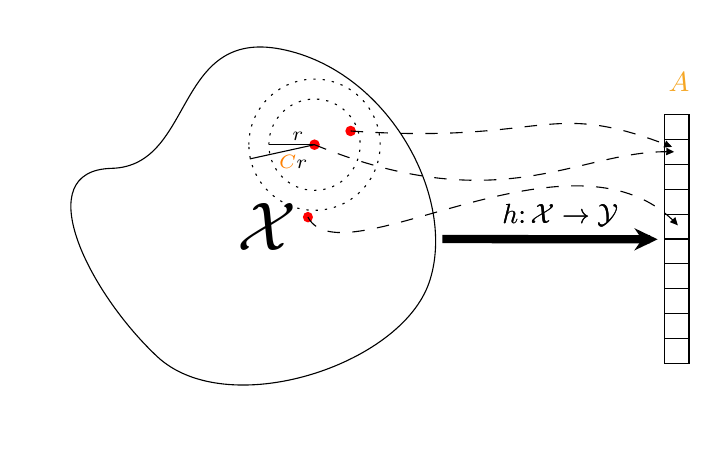
\begin{tikzpicture}[x=0.75pt,y=0.75pt,yscale=-0.6,xscale=0.6]
%uncomment if require: \path (0,300); %set diagram left start at 0, and has height of 300

%Shape: Regular Polygon [id:dp5892453846061058] 
\draw   (200.32,23.52) .. controls (286.72,40.31) and (342.31,143.62) .. (319.3,210.88) .. controls (296.28,278.15) and (156.47,322.59) .. (100.84,270.29) .. controls (45.2,217.99) and (-2.63,120.91) .. (64.25,119.25) .. controls (131.13,117.59) and (113.91,6.73) .. (200.32,23.52) -- cycle ;
%Straight Lines [id:da5940227274966229] 
\draw [line width=3]    (330,176) -- (496.75,176.24) ;
\draw [shift={(502.75,176.25)}, rotate = 180.08] [fill={rgb, 255:red, 0; green, 0; blue, 0 }  ][line width=0.08]  [draw opacity=0] (18.75,-9.01) -- (0,0) -- (18.75,9.01) -- (12.45,0) -- cycle    ;
%Shape: Grid [id:dp5884380060790032] 
\draw  [draw opacity=0] (508,76) -- (528,76) -- (528,276) -- (508,276) -- cycle ; \draw    ; \draw   (508,96) -- (528,96)(508,116) -- (528,116)(508,136) -- (528,136)(508,156) -- (528,156)(508,176) -- (528,176)(508,196) -- (528,196)(508,216) -- (528,216)(508,236) -- (528,236)(508,256) -- (528,256) ; \draw   (508,76) -- (528,76) -- (528,276) -- (508,276) -- cycle ;
%Shape: Circle [id:dp7080915007017408] 
\draw  [draw opacity=0][fill={rgb, 255:red, 255; green, 0; blue, 0 }  ,fill opacity=1 ] (252,89.25) .. controls (252,86.9) and (253.9,85) .. (256.25,85) .. controls (258.6,85) and (260.5,86.9) .. (260.5,89.25) .. controls (260.5,91.6) and (258.6,93.5) .. (256.25,93.5) .. controls (253.9,93.5) and (252,91.6) .. (252,89.25) -- cycle ;
%Curve Lines [id:da44474204475477297] 
\draw  [dash pattern={on 4.5pt off 4.5pt}]  (256.25,89.25) .. controls (415.95,100.2) and (412.13,62.13) .. (512.81,101.4) ;
\draw [shift={(514.33,102)}, rotate = 201.49] [fill={rgb, 255:red, 0; green, 0; blue, 0 }  ][line width=0.08]  [draw opacity=0] (6.25,-3) -- (0,0) -- (6.25,3) -- cycle    ;
%Shape: Circle [id:dp43426133236609155] 
\draw  [draw opacity=0][fill={rgb, 255:red, 255; green, 0; blue, 0 }  ,fill opacity=1 ] (223,100.25) .. controls (223,97.9) and (224.9,96) .. (227.25,96) .. controls (229.6,96) and (231.5,97.9) .. (231.5,100.25) .. controls (231.5,102.6) and (229.6,104.5) .. (227.25,104.5) .. controls (224.9,104.5) and (223,102.6) .. (223,100.25) -- cycle ;
%Curve Lines [id:da27933594579127596] 
\draw  [dash pattern={on 4.5pt off 4.5pt}]  (227.25,100.25) .. controls (379.22,162.13) and (439.54,103.94) .. (513.75,105.92) ;
\draw [shift={(516,106)}, rotate = 182.47] [fill={rgb, 255:red, 0; green, 0; blue, 0 }  ][line width=0.08]  [draw opacity=0] (6.25,-3) -- (0,0) -- (6.25,3) -- cycle    ;
%Shape: Circle [id:dp7752346341981025] 
\draw  [dash pattern={on 0.84pt off 2.51pt}] (190.59,100.25) .. controls (190.59,80) and (207,63.59) .. (227.25,63.59) .. controls (247.5,63.59) and (263.91,80) .. (263.91,100.25) .. controls (263.91,120.5) and (247.5,136.91) .. (227.25,136.91) .. controls (207,136.91) and (190.59,120.5) .. (190.59,100.25) -- cycle ;
%Shape: Ellipse [id:dp3531620947724323] 
\draw  [draw opacity=0][fill={rgb, 255:red, 255; green, 0; blue, 0 }  ,fill opacity=1 ] (217.92,158.42) .. controls (217.92,156.07) and (219.73,154.17) .. (221.97,154.17) .. controls (224.2,154.17) and (226.02,156.07) .. (226.02,158.42) .. controls (226.02,160.76) and (224.2,162.67) .. (221.97,162.67) .. controls (219.73,162.67) and (217.92,160.76) .. (217.92,158.42) -- cycle ;
%Curve Lines [id:da5281745957803201] 
\draw  [dash pattern={on 4.5pt off 4.5pt}]  (221.97,158.42) .. controls (249.53,210.41) and (434.47,76.35) .. (517.75,163.67) ;
\draw [shift={(519,165)}, rotate = 227.43] [fill={rgb, 255:red, 0; green, 0; blue, 0 }  ][line width=0.08]  [draw opacity=0] (6.25,-3) -- (0,0) -- (6.25,3) -- cycle    ;
%Shape: Circle [id:dp18288782111508073] 
\draw  [dash pattern={on 0.84pt off 2.51pt}] (174.55,100.28) .. controls (174.53,71.17) and (198.12,47.56) .. (227.22,47.55) .. controls (256.33,47.53) and (279.94,71.12) .. (279.95,100.22) .. controls (279.97,129.33) and (256.38,152.94) .. (227.28,152.95) .. controls (198.17,152.97) and (174.56,129.38) .. (174.55,100.28) -- cycle ;
%Straight Lines [id:da511433632598341] 
\draw    (227.25,100.25) -- (190.59,100.25) ;
%Straight Lines [id:da9934958278193481] 
\draw    (227.25,100.25) -- (175.33,111.67) ;

% Text Node
\draw (163.5,145.4) node [anchor=north west][inner sep=0.75pt]  [font=\Huge]  {$\mathcal{X}$};
% Text Node
\draw (509.5,39.9) node [anchor=north west][inner sep=0.75pt]    {$\textcolor[rgb]{0.96,0.65,0.14}{\boldsymbol{A}}$};
% Text Node
\draw (376,145.9) node [anchor=north west][inner sep=0.75pt]    {$h\colon \mathcal{X}\rightarrow \mathcal{Y}$};
% Text Node
\draw (376,145.9) node [anchor=north west][inner sep=0.75pt]    {$h\colon \mathcal{X}\rightarrow \mathcal{Y}$};
% Text Node
\draw (207.33,87.73) node [anchor=north west][inner sep=0.75pt]  [font=\scriptsize]  {$r$};
% Text Node
\draw (196.67,106.73) node [anchor=north west][inner sep=0.75pt]  [font=\scriptsize]  {$\orange{C}r$};


\end{tikzpicture}
\end{figure}
%%%%%%%%%%%%%%%%%%%%%%%%%%%%%%%%%%%%%%%%%%%%%%%%%%%%%%%%%%%%%
We will soon see the rationale behind defining this quantity $\rho$: in the meantime, as usual, a few observations:
\begin{itemize}
    \item An LSH family provides a way to control, at a given ``scale'' $r$, the collisions probabilities: sure, you \emph{will} have collisions, but points close to each other (closer than this parameter $r$) are more likely to collide than those much farther apart. This is not as strong as we would like (ideally, we would have wanted the guarantee to be true simultaneously for \emph{all} $r>0$), but this will be good enough.
    \item We would like $p$ to be as large as possible, and $q$ as small as possible: or, put differently, $\rho$ to be as large as we can achieve. This gap is what will allow us to distinguish ``far'' from ``close'' with good enough probability: if $p,q$ are almost equal, this makes our task harder.
    \item LSH families do exist (trivially): one could take $\cY=\cX$ and $\green{\mathcal{H}}$ to be the single function mapping $x$ to itself. This is not interesting at all (it does not save space, time, or anything really), but at least it shows this definition is not impossible to satisfy. What remains is to get more interesting LSH families, with small $\cY$.
\end{itemize}
As a start, we will show how to, given an LSH family for a specific scale $r>0$, solve a ```baby version'' of our Approximate Nearest Neighbour question: that is, we will give a data structure that, after preprocessing, supports the following query, for fixed values of $r>0$ and $\orange{C}>1$.
\begin{framed}
\noindent$\textsc{Query}_r(x)$: given an element $x\in \cX$, return an element $y\in S$, or $\bot$, such that:
\begin{itemize}
    \item If there exists $y^\ast\in S$ such that $\dist{x}{y^\ast} \leq r$, then, with probability at least $9/10$, $\textsc{Query}_r(x)$ returns an element $y\in S$ such that $\dist{x}{y^\ast} \leq \orange{C}\cdot r$;
    \item If $\dist{x}{y} > \orange{C}\cdot r$ for \emph{every} $y\in S$, then, with probability $1$, $\textsc{Query}_r(x)$ returns $\bot$.
    \item Otherwise, any output in $S\cup\{\bot\}$ is allowed.
\end{itemize}
\end{framed}
To solve this ``baby ANN version,'' we will use\dots hash tables. But in addition to a standard, run-of-the-mill good hashing family for the hash tables, we will also use an $(r,\orange{C}, p,q)$-LSH family, which we assume is given to us (we will later show how to design such an LSH family): in what is below, $\purple{k}$ and $\red{\ell}$ are integers, whose values we will carefully choose after analysing the guarantees of our data structure. We first need the following fact, which allows us to ``tune'' the parameters $p,q$ of an LSH family.
\begin{lemma}
    Suppose $\green{\mathcal{H}}$ from $\cX$ to $\cY$ is an $(r,\orange{C}, p,q)$-LSH family, and fix any integer $\red{\ell}\geq 1$. For any $g_1,\dots, g_{\red{\ell}}\in \green{\mathcal{H}}$, define the function $g\colon \cX\to \cY^{\red{\ell}}$ by
    \[
        g(x) = (g_1(x),\dots, g_{\red{\ell}}(x))\in \cY^{\red{\ell}}
    \]
    Then, the resulting family $\green{\mathcal{H}^{(\red{\ell})}} \eqdef \{ (g_1,\dots, g_{\red{\ell}})\colon \cX\to \cY^{\red{\ell}} \}$ is an $(r,\orange{C}, p^{\red{\ell}},q^{\red{\ell}})$-LSH family of size $|\green{\mathcal{H}}|^{\red{\ell}}$ (and as a result has the same sensitivity parameter $\rho$).
\end{lemma}
\begin{proof}
    ``Proof by writing it down.''
\end{proof}
Intuitively, this gives us some flexibility when designing our data structure:\marginnote{``What is the point of this $\red{\ell}$?''} we do not get to choose $p,q$, and would like both (1)~$p$ to be large (better chances of finding close elements, and so smaller probability of failure) \emph{and} (2)~$q$ to be small (fewer ``spurious'' collisions introduced, which will mean better query complexity in our final hash table-based data structure). This parameter $\red{\ell}$ allows us to control (2) (as $q^{\red{\ell}}$ can be made as small as we want), at the price of making (1) worse as well ($p^{\red{\ell}}$ goes down too); fortunately, we will soon introduce our other parameter $\purple{k}$ which will give us control over (1), and so we will be able to achieve both (1) \emph{and} (2) by carefully balancing $\purple{k}$ and $\red{\ell}$.\smallskip

\noindent Let us now actually describe our data structure:
\begin{framed}
\noindent For a fixed, given $r$ (and some $\orange{C}>1$), let $\green{\mathcal{H}}$ be an $(r,\orange{C}, p,q)$-LSH family. Let $g_1,\dots, g_{\purple{k}}\colon \cX\to\cY^{\red{\ell}}$ be hash functions chosen independently from $\green{\mathcal{H}}^{(\red{\ell})}$. Build $\purple{k}$ hash tables $(\orange{A}_1, h_1),\dots, (\orange{A}_{\purple{k}}, h_{\purple{k}})$ with separate chaining, where $h_1,\dots, h_{\purple{k}}\colon \cY\to\cZ$ are $\purple{k}$ independent ``standard'' hash functions from a suitable hashing family.
\begin{itemize}
\item$\textsc{Preprocess}(S)$:
            \begin{algorithmic}
                \ForAll{$x\in S$} \Comment{Insert all $\ns$ elements in all $\purple{k}$ hash tables, using their LSH hashing as keys}
                    \ForAll{$1\leq t\leq \purple{k}$}
                        \State $\orange{A}_{t}[h_t(g_t(x))].\textsc{Insert}(x)$
                    \EndFor
                \EndFor
            \end{algorithmic}

\item$\textsc{Query}_r(x)$: 
            \begin{algorithmic}
                \ForAll{$1\leq t\leq \purple{k}$}
                        \State $L_t\gets \orange{A}_t[h_t(g_t(x))]$ \Comment{List of elements of $S$ colliding with $g_t(x)$ in the $t$-th hash table}
                        \ForAll{$y\in L_t$}
                            \If{$\dist{x}{y} \leq \orange{C}\cdot r$}\label{step:lsh:checkdistance}
                                \State\Return $y$ \Comment{Found one!}
                            \EndIf
                        \EndFor
                \EndFor
                \State\Return $\bot$ \Comment{Did not find any.}
            \end{algorithmic}
\end{itemize}
\end{framed}
Note that we use both the locality-sensitive hash functions $g_t$ \emph{and}\marginnote{``Why do we use two types of hash functions?''} the ``regular'' hash function $h_t$: this is to save space, as if we only used the former we would have the ``locality sensitive'' part, but none of the good guarantees from usual hash functions (small number of hash buckets, along with small collision probability) which allowed us last lecture to argue hash tables were space-efficient. That is, we use two levels of hashing, with two different ``types'' of hash functions:
\begin{itemize}
    \item the first level uses the LSH function $g_t$ to hash elements in a ``locality-sensitive way'' (we \emph{want} close elements to collide, but far elements to go to distinct buckets): this is the main conceptual idea. However, these at-most-$\ns$ resulting elements $S'_t\eqdef \{g_t(x)\}_{x\in S}$ still live in a very big space (\ie $\cY^{\red{\ell}}$), so storing them naively would not be space-efficient; and so,
    \item the second level uses the ``usual'' hash functions $h_t$ to hash this set of ``LSH hashes'' $S'_t$ in a ``standard hash table way'' (we want as few collisions as possible), to save space.
\end{itemize}


We will establish the following guarantees for this data structure, assuming each hash function from $\green{\mathcal{H}}$ can be evaluated in time $T$ and each hash table $\orange{A}_t$ uses space $O(\ns\dims)$:\marginnote{We can improve the $O(\purple{k}\ns\dims)$ space complexity to $O(\purple{k}\ns\log\ns + \ns\dims)$, by only keeping the index of each element $x\in S$ in the data structure along with a separate array containing all of them, to look up where the $i$-th element actually is.}
\begin{theorem}
    The data structure described above for the ``baby version of ANN'' has space complexity $O(\purple{k}\ns\dims + \purple{k}\red{\ell}\dims)$, expected query complexity $O(\purple{k}\red{\ell}T+\purple{k}\ns\dims q^{\red{\ell}})$, and satisfies the correctness requirements as long as $(1-p^{\red{\ell}})^{\purple{k}} \leq \frac{1}{10}$.
\end{theorem}
\begin{proof}
    The space complexity follows from that of the $\purple{k}$ hash tables, each of which using space $O(\ns\dims)$ (we also have to account for the storage of the $\purple{k}$ ``$\red{\ell}$-fold'' LSH hash functions, which we assume can be done with $\red{\ell}\cdot O(\dims)$ bits each). 
    
    The expected query time comes from (1)~evaluating (up to) $\purple{k}$ hash functions $g_1(x),\dots, g_{\purple{k}}(x)$, for a total time $O(\purple{k}\red{\ell}T)$; (2)~for each $1\leq t\leq \purple{k}$, checking the distance to $x$ of every point in the list $L_t$ until we find one that is at distance less than $\orange{C}r$. So we only have to count the expectation number of \emph{false positives} which collide but are far, since a true positive $y$ will be a success, and causes the function to immediately stop and return $y$.  Each distance computation can be done in time $O(\dims)$, and by the LSH guarantee we have on expectation at most 
    \[
        \ns\cdot q^{\red{\ell}}
    \]
    such false positives (points $y$ such that $\dist{x}{y} \geq C\cdot r$ but with $g_t(x)=g_t(y)$); to this, we must add an additional expected $O(1)$ ``standard hash collisions,'' just from the usual guarantees of good hash tables. So that gives us expected query time at most
    \[
        O(\purple{k}\red{\ell}T) + \purple{k}\cdot \Paren{\ns\cdot q^{\red{\ell}}+O(1)} \cdot O(\dims)
        = O(\purple{k}\red{\ell}T+\purple{k}\ns\dims q^{\red{\ell}})
    \]
    assuming, for the last part, that $\ns q^{\red{\ell}} = \Omega(1)$.\footnote{In particular, there is no point in setting $\red{\ell}$ such that $\ns q^{\red{\ell}} \ll 1$, as the $O(1)$ term would then dominate.}

    For the correctness, first observe that the second item is immediate from definition of the algorithm: since Line~\ref{step:lsh:checkdistance} checks the distance is at most $\orange{C}\cdot r$, if every point in $S$ is at distance greater than $\orange{C}\cdot r$ from $x$ then the algorithm will always output $\bot$. The first item is trickier: assume there is a point $y^\ast$ such that $\dist{x}{y^\ast} \leq r$. Then the probability that \emph{none} of the $\purple{k}$ LSH hash functions ``collide'' is at most
    \[
        \probaOf{ \forall t\in[\purple{k}],\; g_t(x) \neq g_t(y^\ast) } \leq (1-p^{\red{\ell}})^{\purple{k}} \leq \frac{1}{10}\,.
    \]
    This is \emph{the} bad event: if it does not happen, then at least one of the $\purple{k}$ hash tables will map $x$ and $y^\ast$ to the same bucket, and so at least one $y$ will pass the test in Line~\ref{step:lsh:checkdistance} (at the very least, $y^\ast$ would: another $y$ might be returned earlier).
\end{proof}
This is encouraging, but we have a \emph{lot} of parameters there. \emph{How should we set $\purple{k}$ and $\red{\ell}$}?
\begin{itemize}
    \item From the second term in the expected query complexity, by setting 
    \begin{equation}
        \label{eq:lsh:setting:l}
        \red{\ell} \eqdef \frac{\log \ns}{\log(1/q)}
    \end{equation}
    we get $q^{\red{\ell}} = 1/\ns$, and so the expected query time becomes $O(\purple{k}\red{\ell}T+\purple{k}\dims)$.
    \item This gives us $p^{\red{\ell}} = 2^{-\red{\ell}\log(1/p)} = \ns^{-\rho}$,\marginnote{``A wild sensitivity parameter $\rho$ appears''} and to satisfy the correctness condition 
    \[
        (1-p^{\red{\ell}})^{\purple{k}} \leq \frac{1}{10}
    \]
    it is then sufficient (and necessary) to set\marginnote{Check it!}
    \begin{equation}
        \label{eq:lsh:setting:k}
        \purple{k} = O(n^{\rho})
    \end{equation}
\end{itemize}
This finally gives us the following (recalling that $\log\ns \ll \dims$ to simplify the query complexity):
\begin{corollary}
    With the settings of $\purple{k},\red{\ell}$ from~\cref{eq:lsh:setting:l,eq:lsh:setting:k} and assuming $q,T=\Theta(1)$, the data structure for the ``baby version of ANN'' has space complexity $O(\ns^{1+\rho}\dims)$ and expected query complexity $O(\ns^\rho\dims)$.
\end{corollary}
This is quite good: the space is only ``mildly worse'' than the necessary $\ns\dims$, and query complexity is \emph{sublinear} in $\ns$, since $\rho < 1$!\bigskip

\textbf{But}\dots this was just a ``baby'' version of our problem: this did not solve the ANN question itself! Thankfully, there is a `simple'' reduction from this version (where $r$ is ``hardcoded'') to the general case:
\begin{theorem}
    Suppose that, for every $0 < r\leq \dims$, we have a data structure for the ``baby'' version of ANN with scale parameter $r$ and parameter $\orange{C}>0$, with space complexity $S(\ns,\dims)$, expected query complexity $T(\ns,\dims)$ and probability of failure $\errprob$ per query. Then there is a data structure for ANN with parameter $2\orange{C}$, space complexity $O(S(\ns,\dims)\log^2\ns)$, expected query complexity $O(T(\ns,\dims)\log\ns)$, and probability of failure $\errprob\log\ns$ per query..
\end{theorem}
\begin{proof}
    This reduction is quite involved, and was shown in Theorem~2.9 of~\cite{HarPeledIM12}. In the tutorial, you will see a much simpler version, losing instead a logarithmic factor in the ``aspect ratio''
    \[
        \Delta \eqdef \frac{\max_{x,x'} \dist{x}{x'}}{\min_{x,x'} \dist{x}{x'}}
    \]
    using, essentially, a doubling search over $r$.
\end{proof}
At this point, we know what to do if we are \emph{given} an LSH family for the metric space $(\cX,\operatorname{dist})$ we care about~--~and the smaller the parameter $\rho$ of that LSH family is, the better the query times and space complexity we will obtain are. Which brings a very natural question:
\begin{framed}
   \noindent Are there good  LSH families for the metric spaces we care about?
\end{framed}
\noindent We will give two examples, showing that the answer is (mostly) ``yes.''
\subsection{Example: Hamming space}
The first example is that of the \emph{Hamming space of dimension $\dims$}, which, again, is just a fancy way of saying ``the universe of $\dims$-bit strings where the distance between two $x,x'\in \cX = \bool^\dims$ is the number of bits in which they differ.''

What will be the LSH family? The simplest thing one could think of: $\green{\mathcal{H}}$ will just be the set of $\dims$ functions
\[
    h_i\colon \bool^\dims\to \bool, \qquad 1\leq i\leq \dims
\]
where $h_i(x) = x_i$ just ``hashes'' a string $x$ to its $i$-bit. That's all! One can then verify that, for every $1\leq r\leq \dims$ and $\orange{C}>1$,\marginnote{If $\orange{C}r > \dims$ the guarantee is trivially true.}
    \begin{itemize}
        \item If $\dist{x}{x'} \leq r$, then $\probaDistrOf{h\sim \green{\mathcal{H}}}{h(x)=h(x')} \geq 1-\frac{r}{\dims}$;
        \item If $\dist{x}{x'} \geq \orange{C}r$, then $\probaDistrOf{h\sim \green{\mathcal{H}}}{h(x)=h(x')} \leq 1-\frac{\orange{C}r}{\dims}$;
    \end{itemize}
and so this $\green{\mathcal{H}}$ is an $(r,\orange{C}, p,q)$-LSH family for $p\eqdef 1-\frac{r}{\dims}, q\eqdef 1-\frac{\orange{C}r}{\dims}$, with size $|\green{\mathcal{H}}|=\dims$ and sensitivity
\begin{equation}
    \rho = \frac{\log\Paren{1-\frac{r}{\dims}}}{\log\Paren{1-\frac{\orange{C}r}{\dims}}} \approx \frac{1}{\orange{C}}\,.
\end{equation}
\noindent(as a side note, it has been shown that $\rho = \Theta(1/\orange{C})$ is the best one can get for the Hamming space.)
\subsection{Example: Euclidean space ($\lp[2]$ distance)}
What about the Euclidean space? Recycling is good, so we may want to use some of the ideas behind the JL Lemma to design a good LSH Family. Fortunately, this is possible: pick a random vector $\green{g}\sim\cN(0,I_{\dims})$, and set
\begin{equation}
    h_{\green{g}}(x) = \operatorname{sign}(\langle \green{g}, x \rangle) \in \{-1,1\}
\end{equation}
(that is, pick a random gaussian vector $\green{g}$, and take the sign of the inner product between $\green{g}$ and $x$). One can show\footnote{And you will in the tutorial.} that, for every $r>0$ and $\orange{C}>1$, this gives an LSH family with sensitivity parameter
\begin{equation}
    \rho \leq \frac{1}{\orange{C}}\,.
\end{equation}
Interestingly, this is not optimal! For the Euclidean space, more involved constructions are able to obtain LSH families with sensitivity parameter $\rho = O(1/\orange{C}^2)$.


%https://www.cs.princeton.edu/~hy2/teaching/fall22-cos521/notes/NNS%20&%20LSH.pdf
% https://cs368-stanford.github.io/spring2022/lectures/lec17.pdf

% Some other lecture notes:
% https://www.cs.toronto.edu/~anikolov/CSC473W20/Lectures/LSH.pdf
% https://www.cs.princeton.edu/courses/archive/fall18/cos521/Lectures/lec12.pdf
% https://cs368-stanford.github.io/spring2022/lectures/lec16.pdf
% https://cs368-stanford.github.io/spring2022/lectures/lec17.pdf (mentions the Kane-Nelson faster JL)
% https://www.cs.cmu.edu/~15451-s19/lectures/lec22-nearest-neighbor.pdf

% https://www.cs.columbia.edu/~andoni/LSH/

\chapter{Lecture 8: Streaming and Sketching I}
\begin{quotation}\itshape
``In low-space, nobody can remember your stream.''
\end{quotation}

\begin{framed}
    We will follow for this chapter the (excellent) lecture notes by Amit Chakrabarti [AC], available at \url{https://www.cs.dartmouth.edu/~ac/Teach/data-streams-lecnotes.pdf}.
\end{framed}
%%%%%%%%%%%%%%%%%%%%%%%%%%%%%%%%%%%%%%%%%%%%%%%%%%%%%%%%%%%%%%%%%%%%%%%%%%%%%%%
\section{The Basic Setup}
We will specifically focus on one-pass algorithms, unless specified otherwise. $\green{m}$ denotes the length of the stream 
\[
\sigma = \langle a_1,\dots, a_{\green{m}} \rangle
\]
where each $a_i$ belongs to the universe $\cX$ of size $\ns$.\marginnote{Note that this notation is swapped with respect to the previous lectures, in other to match the lecture notes.} We do not impose any bound on the time complexity of our algorithms, but we will enforce that they use very little memory (space), with space complexity denoted by $\purple{s}$. We will aim for 
\[
\purple{s} = o(\min(\green{m},\ns))
\]
and would love to use much less, ideally 
\[
\purple{s} = O(\log \green{m} + \log\ns)
\]
or, if not, $\purple{s} = \poly(\log \green{m}, \log \ns)$. To do so, we will allow for randomised algorithms \emph{and} approximation algorithms, where the quality of the approximation will be controlled by a parameter $\dst > 0$, usually thought of as an (arbitrarily) small fixed constant.

\section{The Majority Problem}\marginnote{Chapter 1 of [AC]}
To begin, consider the (seemingly) very simple question of deciding whether there is \emph{one} element that appears at least half the time in the stream: that is, some  $j\in [\ns]$ whose \emph{frequency} $f_j$, defined as 
\[
    f_j \eqdef \sum_{i=1}^{\green{m}} \indicSet{a_i = j}
\]
satisfies $f_j \geq \frac{\green{m}}{2}$. This is the \textsc{Majority} problem: \marginnote{Of course, there are \emph{at most} two such elements, and at most one if we define the question as ``is there some $j$ such that $f_j > \green{m}/2$?'' The issue is that we do not know \emph{a priori} which one(s) of the $\ns$ elements could be the majority element(s).} at first glance, this seems very easy! Yet, spending some time thinking about it, you should convince yourself than it is surprisingly non-trivial to solve it using little memory.

The first algorithm we will see, due to Misra and Gries~\cite{MisraG82}, is quite incredible in that regard: what it does is solving, \emph{deterministically}, a related (and more general) version of this question, which we will return into more detail in the next chapter: the question of \emph{frequency estimation}, which asks to approximate the frequency $f_j$'s, not just decide which ones are at least $\green{m}/2$.
\begin{theorem}
    The \textsc{Misra-Gries} algorithm (\cref{algo:misra:gries}) is a \emph{deterministic} one-pass algorithm which, for any given parameter $\dst\in(0,1]$, provides $\hat{f}_1,\dots, \hat{f}_{\ns}$ of all element frequencies such that
    \[
           f_j - \dst \green{m} \leq \hat{f}_j \leq f_j, \qquad j\in[\ns]
    \]
    with space complexity $\purple{s} = O(\log(\green{m}\ns)/\dst)$. (In particular, it can be used to solve the \textsc{Majority} problem in two passes.)
\end{theorem}
An interesting observation here is that of course the algorithm cannot compute explicitly $\ns$ values $\hat{f}_1,\dots, \hat{f}_{\ns}$: this by itself would take $\Omega(\ns)$ space. What it does is \emph{implicitly} do so, by only storing the values $\hat{f}_j$'s that are \emph{non-zero} (and making sure there are very few of them, only $O(1/\dst)$). Which makes sense, since we should not have many more non-zero estimates than this: after all, there can only be at most $1/\dst$ element $j\in[\ns]$ such that $f_j \geq \dst \green{m}$ (\ie which appear at least an $\dst$ fraction of the time in the stream)!
\begin{algorithm}
    \begin{algorithmic}[1]
    \Require Parameter $\dst\in(0,1]$
    \State $\red{A} \gets \emptyset$ \Comment{Use, \eg a self-balancing binary search tree (BST)}
    \State Set $\purple{k} \gets \clg{1/\dst}$
    \ForAll{$1\leq i\leq \green{m}$}
        \State Get item $a_i = j\in [\ns]$
        \If{$\red{A}[j] > 0$} \Comment{$j$ is in the BST}
            \State $\red{A}[j]  \gets \red{A}[j] + 1$ \label{algo:misra:gries:increment2}
        \ElsIf{$\red{A}[j] = 0$ \textbf{and} $\abs{\red{A}} < \purple{k}-1$}
            \State $\red{A}[j]  \gets 1$ \label{algo:misra:gries:increment1}
        \ElsIf{$\red{A}[j] = 0$ \textbf{and} $\abs{\red{A}} = \purple{k}-1$}
            \ForAll{$j' \in \red{A}$}   \Comment{Loop over all $j'$ such that $\red{A}[j'] > 0$}
                \State $\red{A}[j']  \gets \red{A}[j'] - 1$ \Comment{If $\red{A}[j']$ reaches $0$, remove it from $\red{A}$} \label{algo:misra:gries:decrement}
            \EndFor
        \EndIf
    \EndFor
    \Ensure On query $j\in[\ns]$, \Return $\red{A}[j]$
    \end{algorithmic}
    \caption{The \textsc{Misra-Gries} algorithm. Only store in $\red{A}$: if $\red{A}[j]$ does not exist, it is $0$. Instead of a BST, one could use a linked list, for instance: this would have the same space complexity, but a larger update time at each step.}\label{algo:misra:gries}
\end{algorithm}
\begin{proof}
First, note that since $\red{A}$ never stores more $\purple{k} = O(1/\dst)$ elements, each of them taking $O(\log\ns + \log\green{m})$ bits (for the index of the element, and its current count), the space $\purple{s}$ is bounded as
\[
    \purple{s} = \bigO{\frac{\log(\green{m}\ns)}{\dst}}
\]
as claimed. 

To prove correctness, fix any $j\in[\ns]$. Since $\red{A}[j]$ can only be incremented (on Line~\ref{algo:misra:gries:increment1} or~\ref{algo:misra:gries:increment2}) when element $j$ appears in the stream, we have, at the end of the stream,
\[
    \hat{f}_j = \red{A}[j] \leq f_j\,.
\]
For the other inequality (the lower bound), we need to get a grasp on the number of times $\red{A}[j]$ is decremented, which can only happen in Line~\ref{algo:misra:gries:decrement}. Every time this line is reached, this means that (1)~nothing else happens in this step (no increment to $\red{A}[j]$), and (2)~exactly $\purple{k}-1$ other counters are decremented (in the \textbf{for all} loop).

We can see (1), conceptually, as one increment to $\red{A}[j]$ immediately followed by a decrement to $\red{A}[j]$: thinking of it this way allows us to say that $\red{A}[j]$ is incremented every time $j$ appears in the stream~--~but sometimes, it is decremented immediately after as well, and lets us combine (1) and (2) to say that every time Line~\ref{algo:misra:gries:decrement} is reached, \emph{exactly} $\purple{k}$ decrements are performed in $\red{A}$.
Given that every increment uniquely corresponds to one of the $\green{m}$ steps,this means that each execution of Line~\ref{algo:misra:gries:decrement} corresponds to a disjoint chunk of $\purple{k}$ steps: when the increments to the $\red{A}[j']$'s had happened. But there are only $\green{m}$ steps in total, so if each decrement ``burns'' $\purple{k}$ of them, there can be at most $\frac{\green{m}}{\purple{k}}$ decrements steps! This shows that
\[
    \hat{f}_j = \red{A}[j] \geq f_j - \frac{\green{m}}{\purple{k}}\,,
\]
which, given the value of $\purple{k}$, implies $\hat{f}_j \geq f_j - \dst \green{m}$.\smallskip

To see how the ``In particular'' statement follows, consider applying the \textsc{Misra-Gries} algorithm with $\dst = 1/4$, and at the end of the first pass considering the set $S\subseteq [\ns]$ of elements for which $\hat{f}_j \geq \frac{1}{4}\green{m}$. If $j^\ast$ is a majority element, then
\[
    \hat{f}_j \geq f_j - \dst \green{m} \geq \frac{1}{2}\green{m} - \frac{1}{4}\green{m} = \frac{1}{4}\green{m}\,,
\]
so $j^\ast \in S$. Conversely, if $j\in S$, then
\[
    f_j  \geq \hat{f}_j \geq \frac{1}{4}\green{m}\,,
\]
and so there can be at most $\frac{\green{m}}{(1/4)\green{m}} = 4$ elements in $S$. So keeping $S$ in memory only takes $4\cdot O(\log\ns)=O(\log\ns)$ bits. Then, all that remains to do is, in the \emph{second} pass, count \emph{exactly} the number of times each elements $j\in S$ appears, and check if that's at least $\green{m}/2$. Each such counter takes $O(\log\green{m})$ bits, and there are only (at most) $4$ counters to maintain now.
\end{proof}
%%%%%%%%%%%%%%%%%%%%%%%%%%%%%%%%%%%%%%%%%%%%%%%%%%%%%%%%%%%%%%%%%%%%%%%%%%%%%%%
\section{The Approximate Counting Problem}\marginnote{Chapter 4 of [AC]}
We will describe and analyse the Morris Counter algorithm, due to, well, Morris~\cite{Morris78}, which provides a constant-factor estimate of the number of elements of the stream: that is, an $F_1$ estimator. Put differently, at each time step $1\leq t\leq \green{m}$, we are told if some event happened ($a_i=1$) or not ($a_i=0$): the goal is to estimate how many events happened in total, \ie the number $\blue{d} = \sum_{i=1}^{\green{m}} a_i$.

\begin{algorithm}
    \begin{algorithmic}[1]
    \State $\blue{x} \gets 0$
    \ForAll{$1\leq i\leq \green{m}$}
        \State Get item $a_i\in \bool$
        \If{$a_i = 1$} 
                \State $r_i \gets \bernoulli{{1}/{2^{\blue{x}}}}$ \Comment{Independent of previous choices.}
                \State $\blue{x} \gets \blue{x} + r_i$
        \EndIf
    \EndFor
    \State \Return $\blue{\widehat{d}} \gets 2^{\blue{x}}-1$
    \end{algorithmic}
    \caption{The \textsc{Morris Counter} algorithm.}\label{algo:morris}
\end{algorithm}
The space complexity is a little annoying to bound: we \emph{expect} $\blue{x}$ to never exceed $\log_2\green{m}$, since $\blue{d}$ is at most $\green{m}$ by definition and we should have $2^{\blue{x}}\approx \blue{d}$. But there is a very, very small chance that all Bernoullis turn out to be $1$, in which case $\blue{x}$ could become as big as $\green{m}$! This would make no sense, and also mean we would need $O(\log \green{m})$ bits to store $\blue{x}$, exactly what we do not want to pay. \emph{However},\marginnote{If $\blue{x}$ ever exceeds this value, the algorithm can just abort: this only adds a vanishing small amount to the probability of error.}  one can show that with overwhelming probability $\blue{x}$ remains at most $O(\log\green{m})$, and so the space complexity required is only $\purple{s} = O(\log \log \green{m})$.

The proof of correctness of~\cref{algo:morris} relies on the key lemma below, analysing the expectation and variance of $\blue{\widehat{d}}$:
\begin{lemma}
    The random variable $\blue{\widehat{d}}$ defined in~\cref{algo:morris} satisfies
    \[
        \expect{\blue{\widehat{d}}} = \blue{d}
    \]
    and
    \[
        \var[\blue{\widehat{d}}] = \frac{\blue{d}(\blue{d}-1)}{2}
    \]
\end{lemma}
\begin{proof}
    Define $\blue{C}_i$, for $1\leq i\leq \green{m}$, as the value of $2^{\blue{x}}$ in~\cref{algo:morris} at the end of step $i$; so that $\blue{C}_0 = 2^0=1$ and $\blue{\widehat{d}} = \blue{C}_{\green{m}}-1$.

    For any $1\leq i < \green{m}$, we then have
    \[
    \blue{C}_{i+1} = \begin{cases}
        2\cdot \blue{C}_i &\text{if } a_{i+1} = 1\text{ and } r_{i+1}=1\\
        \blue{C}_i &\text{otherwise}
    \end{cases}
    \]
    which we can rewrite as $\blue{C}_{i+1} = (1+ a_{i+1} r_{i+1})\blue{C}_i$. Recalling that $r_{i+1}\sim \bernoulli{{1}/{\blue{C}_i}}$ gives us
    \[
    \expectCond{\blue{C}_{i+1}}{\blue{C}_i}
    = (1+a_{i+1}\expectCond{r_{i+1}}{\blue{C}_i})\cdot \blue{C}_i
    = \Paren{1+\frac{a_{i+1}}{\blue{C}_i}}\cdot \blue{C}_i
    = \blue{C}_i + a_{i+1}
    \]
    and, by the Law of Total Expectation,
    \[
    \expect{\blue{C}_{i+1}}
    = \expect{\expectCond{\blue{C}_{i+1}}{\blue{C}_i}}
    = \expect{\blue{C}_i} + a_{i+1}\,.
    \]
    This gives us
    \[
        \expect{\blue{C}_{\green{m}}}
        = \expect{\blue{C}_0}+\sum_{i=0}^{\green{m}-1} \Paren{\expect{\blue{C}_{i+1}}-\expect{\blue{C}_i}}
        = 1 + \sum_{i=0}^{\green{m}-1} a_{i+1}
        = 1 + \blue{d}
    \]
    showing that $\expect{\blue{\widehat{d}}} = \blue{d}$. The above actually showed the more general statement that
    \begin{equation}
        \label{eq:morris:vexpectation:step}
        \expect{\blue{C}_{i}} = 1 + \sum_{j=1}^{i} a_{j}, \qquad 1\leq i\leq \green{m}\,,
    \end{equation}
    which we will use very soon.
    
    To compute the variance, we similarly analyse $\expect{\blue{C}_{\green{m}}^2}$: For any $1\leq i < \green{m}$,
    \begin{align*}
    \expectCond{\blue{C}_{i+1}^2}{\blue{C}_i}
    &= \expectCond{(1+a_{i+1}r_{i+1})^2}{\blue{C}_i}\cdot \blue{C}_i^2\\
    &= \Paren{1+\frac{a_{i+1}(2+a_{i+1})}{\blue{C}_i}}\cdot \blue{C}_i^2 \\
    &= \blue{C}_i^2 + a_{i+1}(2+a_{i+1})\blue{C}_i
    \end{align*}
    where the second equality follows from expanding the square and computing the expectation. Again, by the Law of Total Expectation,
    \begin{align*}
    \expect{\blue{C}_{i+1}^2}
    &= \expect{\expectCond{\blue{C}_{i+1}^2}{\blue{C}_i}} 
    = \expect{\blue{C}_i^2} + a_{i+1}(2+a_{i+1})\expect{\blue{C}_i} \\
    &= \expect{\blue{C}_i^2} + a_{i+1}(2+a_{i+1})\Paren{1 + \sum_{j=1}^{i} a_{j}} \tag{By~\cref{eq:morris:vexpectation:step}} \\
    &= \expect{\blue{C}_i^2} + 3a_{i+1}\sum_{j=1}^{i+1} a_{j}
    \end{align*}
    where that last step is completely magical, but ``immediate in hindsight'' by checking the two possible cases: $a_{i+1}(2+a_{i+1})\Paren{1 + \sum_{j=1}^{i} a_{j}} = 3a_{i+1}\Paren{a_{i+1} + \sum_{j=1}^{i} a_{j}}$ for both $a_{i+1}=0$ and $a_{i+1}=1$. This gives us
    \begin{align*}
    \expect{\blue{C}_{\green{m}}^2}
    &= \expect{\blue{C}_0^2} + 3\sum_{i=0}^{\green{m}-1}a_{i+1}\sum_{j=1}^{i+1} a_{j}
    = 1 + 3\sum_{i=1}^{\green{m}}\sum_{j=1}^{i} a_{i}a_{j} \\
    &= 1 + 3\cdot \frac{1}{2}\Paren{\Paren{\sum_{i=1}^{\green{m}} a_i}^2 + \sum_{i=1}^{\green{m}} a_i^2} \\
    &= 1 + 3\cdot \frac{1}{2}\Paren{\blue{d}^2 + \blue{d}}
    \end{align*}
    (recalling, for the last step, that $a_i^2=a_i$ for all $i$, since $a_i \in\bool$). Since $\expect{\blue{C}_{\green{m}}}^2 = \blue{d}+1$, we finally get
    \[
    \var[\blue{C}_{\green{m}}] = 
    1 + 3\cdot \frac{1}{2}\Paren{\blue{d}^2 + \blue{d}}
    - (\blue{d}+1)^2 = \frac{\blue{d}^2 - \blue{d}}{2}\,,
    \]
    as claimed.
\end{proof}

While this $\bigTheta{\blue{d}^2}$ variance by itself is not good enough to obtain an accurate estimate with high constant probability using Chebyshev's inequality, averaging $k=O(1/\dst^2)$ independent copies of the Morris Counter enables us to bring down the variance by this factor, leading to a $(1+\dst)$-estimate with high (constant) probability. Using the median trick afterwards (running $T=O(\log(1/\errprob))$ copies of this improved-variance algorithm, and taking the median result) gives a high-probability result, leading to the following:
\begin{theorem}
    The medians-of-means version of the \textsc{Morris Counter} is a \emph{randomised} one-pass algorithm which, for any given parameters $\dst, \errprob\in(0,1]$, provides an estimate $\blue{\widehat{d}}$ of the number $\blue{d}$ of non-zero elements of the stream such that
    \[
           \probaOf{ (1-\dst)\blue{d} \leq \blue{\widehat{d}} \leq (1+\dst) \blue{d} } \geq 1-\errprob
    \]
    with space complexity 
    \[
        \purple{s} = \bigO{ \frac{\log\log\green{m}}{\dst^2}\cdot \log\frac{1}{\errprob} }
    \]
    that is, \emph{doubly logarithmic} in $\green{m}$.
\end{theorem}
Again, maintaining an exact counter would take $O(\log\green{m})$ bits: this is an exponential improvement! And yet, \emph{we can do better.} Instead of using the median-of-means technique, we can be more careful about the algorithm itself: where we incremented $\blue{x}$ with probability $1/2^{\blue{x}}$ and returned $2^{\blue{x}}-1$, we will, for a suitable choice of $\alpha = \alpha(\dst,\errprob) > 0$, increment it with with probability $1/(\alpha(1+\alpha)^{\blue{x}})$ and return $(1+\alpha)^{\blue{x}}-1$. We will see the details in the tutorial, leading to this (much) improved bound:
\begin{theorem}
    The ``careful'' version of \textsc{Morris Counter} is a \emph{randomised} one-pass algorithm which, for any given parameters $\dst, \errprob\in(0,1]$, provides an estimate $\blue{\widehat{d}}$ of the number $\blue{d}$ of non-zero elements of the stream such that
    \[
           \probaOf{ (1-\dst)\blue{d} \leq \blue{\widehat{d}} \leq (1+\dst) \blue{d} } \geq 1-\errprob
    \]
    with space complexity 
    \[
        \purple{s} = \log\log\green{m} + \bigO{ \log\frac{1}{\dst}+\log\frac{1}{\errprob} }
    \]
    that is, doubly logarithmic in $\green{m}$ \emph{and logarithmic in $1/\dst$}.
\end{theorem}
%%%%%%%%%%%%%%%%%%%%%%%%%%%%%%%%%%%%%%%%%%%%%%%%%%%%%%%%%%%%%%%%%%%%%%%%%%%%%%%
\section{The Distinct Elements Problem}\marginnote{Chapters 2 and 3 of [AC]}
We start this section with the \textsc{Tidemark} algorithm, due to Alon, Matias and Szegedy (AMS), which provides a constant-factor estimate of the number of distinct elements of the stream: that is, an $F_0$ estimator. In this section, we define $\blue{d}$ as this number of distinct elements, \ie
\[
    \blue{d} = \sum_{j\in[\ns]}\indicSet{f_j > 0}
\]

In what follows, for a given positive integer $k$, $\operatorname{zeros}(k)$ denotes the largest power of 2 which divides $k$, or, equivalently, the number of trailing zeroes in the binary representation of $k$.
\begin{algorithm}
    \begin{algorithmic}[1]
    \State Pick $h\colon[\ns]\to[\ns]$ from a strongly universal hashing family
    \State $\blue{z}\gets 0$
    \ForAll{$1\leq i\leq \green{m}$}
        \State Get item $a_i \in [\ns]$
        \If{$\operatorname{zeros}(h(a_i)) \geq \blue{z}$}
            \State $\blue{z}\gets \operatorname{zeros}(h(a_i))$
        \EndIf
    \EndFor
    \State \Return $\blue{\widehat{d}}\gets \sqrt{2}\cdot  2^{\blue{z}}$
    \end{algorithmic}
    \caption{The \textsc{Tidemark} algorithm}\label{algo:tidemark}
\end{algorithm}
The space complexity of~\cref{algo:tidemark} is 
\[
    \purple{s} = \bigO{\log\ns}
\]
as all that is needed is storing the hash function ($\bigO{\log\ns}$ bits, for a suitable strongly universal hash family) and $1\leq \blue{z}\leq \log_2\ns$ (which takes $\bigO{\log\log\ns}$ bits). To analyse the correctness of the algorithm (and the quality of the estimate it outputs), define the random variables
\[
    Y_r \eqdef \sum_{\substack{j\in[\ns]\\ f_j > 0}} \indicSet{\operatorname{zeros}(h(j)) \geq r}, \qquad r \geq 0
\]
(where the randomness is over the choice of the hash function $h$). One can check that, by definition,
\[
    Y_r \geq 1 \Leftrightarrow \blue{z} \geq r
\]
for every integer $r\geq 0$. Moreover,
\[
    \expect{Y_r} = \sum_{\substack{j\in[\ns]\\ f_j > 0}} \probaOf{\operatorname{zeros}(h(j)) \geq r} = \sum_{\substack{j\in[\ns]\\ f_j > 0}} \frac{1}{2^r} = \frac{\blue{d}}{2^r}
\]
where we used the fact that each $h(j)$ is uniformly distributed to write that $\probaOf{\operatorname{zeros}(h(j)) \geq r} = \probaOf{2^r \text{ divides } h(j)} = \frac{1}{2^r}$. Similarly, using pairwise independence,
\[
    \var[Y_r] = \sum_{\substack{j\in[\ns]\\ f_j > 0}} \var[\indicSet{\operatorname{zeros}(h(j)) \geq r}]  \leq \sum_{\substack{j\in[\ns]\\ f_j > 0}} \frac{1}{2^r} = \frac{\blue{d}}{2^r}
\]
the inequality using $\var[X] \leq \expect{X^2}$ and the fact that $X^2=X$ when $X$ is an indicator random variable. Using these two facts, for every $r\geq 0$,
\begin{itemize}
    \item $\probaOf{\blue{z} \geq r} = \probaOf{Y_r \geq 1} \leq \expect{Y_r} = \frac{\blue{d}}{2^r}$ by Markov;
    \item $\probaOf{\blue{z} \leq r} = \probaOf{Y_{r+1} = 0 } \leq \frac{\var[Y_{r+1}] }{\expect{Y_{r+1}}^2} \leq \frac{2^{r+1}}{\blue{d}}$ by Chebyshev,
\end{itemize}
using that $\probaOf{Y_{r+1} = 0 } \leq \probaOf{|Y_{r+1} - \expect{Y_{r+1}}| \geq \expect{Y_{r+1}} }$. This is all we need! Setting $\orange{C} \eqdef 3\sqrt{2}$,
\[
\probaOf{\blue{\widehat{d}} \geq \orange{C}\cdot \blue{d}}
\leq \probaOf{\blue{z} \geq \clg{\log_2(\orange{C}\cdot \blue{d}/\sqrt{2})}}
\leq \frac{\sqrt{2}\blue{d}}{\orange{C}\blue{d}}  = \frac{1}{3}
\]
while
\[
\probaOf{\blue{\widehat{d}} \leq \blue{d}/\orange{C}}
\leq \probaOf{\blue{z} \leq \flr{\log_2(\blue{d}/(\sqrt{2}\orange{C}))}}
\leq \frac{2\blue{d}}{\sqrt{2}\orange{C}\blue{d}}  = \frac{1}{3}
\]

Combining the above with the median trick, we readily get:
\begin{theorem}
    The (median trick version of the) \textsc{Tidemark} (AMS) algorithm  is a \emph{randomised} one-pass algorithm which, for any given parameter $\errprob\in(0,1]$, provides an estimate $\blue{\widehat{d}}$ of the number $\blue{d}$ of distinct elements of the stream such that, for some absolute constant $\orange{C}>0$,
    \[
           \probaOf{ \frac{1}{\orange{C}}\cdot\blue{d} \leq \blue{\widehat{d}} \leq \orange{C} \cdot \blue{d} } \geq 1-\errprob
    \]
    with space complexity 
    \[
        \purple{s} = \bigO{ \log \ns \cdot \log\frac{1}{\errprob} }\,.
    \]
\end{theorem}
This is not bad, but can we achieve estimation factor arbitrarily close to one, say, $1+\dst$? The answer is yes: the following algorithm, due to  Bar-Yossef, Jayram, Kumar, Sivakumar and Trevisan (BJKST), does exactly that.

\begin{algorithm}
    \begin{algorithmic}[1]
    \Require Parameter $\dst\in(0,1]$
    \State Set $\purple{k} \gets O(\log^2\ns/\dst^4)$, $\purple{T} \gets \Theta(1/\dst^2)$
    \State Pick $h\colon[\ns]\to[\ns]$ from a strongly universal hashing family
    \State Pick $g\colon[\ns]\to[\purple{k}]$ from a strongly universal hashing family%\marginnote{Check if strongly is necessary}
    \Statex
    \State $\blue{z}\gets 0$, $\red{B}\gets \emptyset$
    \ForAll{$1\leq i\leq \green{m}$}
        \State Get item $a_i \in [\ns]$
        \If{$\operatorname{zeros}(h(a_i)) \geq \blue{z}$}
            \State $\red{B} \gets \red{B}\cup \{(g(a_i), \operatorname{zeros}(h(a_i)))\}$
            \While{$|\red{B}| \geq \purple{T}$}
                \State $\blue{z}\gets \blue{z}+1$
                \State Remove every $(a,b)$ with $b< \blue{z}$ from $\red{B}$
            \EndWhile
        \EndIf
    \EndFor
    \State \Return $|\red{B}|\cdot  2^{\blue{z}}$
    \end{algorithmic}
    \caption{The \textsc{BJKST} algorithm}
\end{algorithm}

\begin{theorem}
    The (median trick version of the) \textsc{BJKST} algorithm  is a \emph{randomised} one-pass algorithm which, for any given parameters $\dst,\errprob\in(0,1]$, provides an estimate $\blue{\widehat{d}}$ of the number $\blue{d}$ of distinct elements of the stream such that, for some absolute constant $\orange{C}>0$,
    \[
           \probaOf{ (1-\dst)\cdot\blue{d} \leq \blue{\widehat{d}} \leq (1+\dst)\blue{d} } \geq 1-\errprob
    \]
    with space complexity 
    \[
        \purple{s} = \bigO{ \Paren{\log \ns + \frac{\log(1/\dst) + \log\log\ns}{\dst^2} }\cdot \log\frac{1}{\errprob} }\,.
    \]
\end{theorem}
This is pretty good, but\dots \emph{Is it optimal?}

\chapter{Lecture 9: Streaming and Sketching II}
\begin{framed}
    We will follow for this chapter the (excellent) lecture notes by Amit Chakrabarti [AC], available at \url{https://www.cs.dartmouth.edu/~ac/Teach/data-streams-lecnotes.pdf}.
\end{framed}
%%%%%%%%%%%%%%%%%%%%%%%%%%%%%%%%%%%%%%%%%%%%%%%%%%%%%%%%%%%%%%%%%%%%%%%%%%%%%%%
\section{Sketching}\marginnote{Chapter 5.2 of [AC]}
A sketching algorithm is the response to the following very natural question: 
\begin{framed}\itshape
    If I run two instances of a streaming algorithm for problem $\mathcal{P}$ on a stream $\sigma_1$ and on a stream $\sigma_2$, can I combine their outputs to get the same result as if I had run my algorithm for $\mathcal{P}$ on the stream $\sigma_1\circ\sigma_2$?
\end{framed}
This sounds very desirable, as this allows to stop an algorithm, distribute it across multiple servers or subsets of a stream, and still be able to recombine everything. 

What is even \emph{more} appealing is a \emph{linear} sketching algorithm, where the (sketch) output of the algorithm is just a linear function of the input stream (into a lower-dimensional space), and where ``combining their outputs'' just means\dots summing them up.
%%%%%%%%%%%%%%%%%%%%%%%%%%%%%%%%%%%%%%%%%%%%%%%%%%%%%%%%%%%%%%%%%%%%%%%%%%%%%%%
\section{Back to Frequent Elements!}
Remember that in the previous lecture, we saw the \textsc{Misra--Gries} algorithm which allowed us to compute deterministically, in one pass, an additive approximation of all the $\ns$ frequencies of a given stream $\sigma$:
\[
    \blue{f}_j - \dst\green{m} \leq \blue{\widehat{f}}_j \leq \blue{f}_j, \qquad \text{ for all } j\in[\ns]
\]
using space $\purple{s} = \bigO{\log(\green{m}\ns)/\dst}$. We will see in the tutorial that this is actually already a sketching algorithm! 

It suffers from two possible issues, however: first, it only works in the ``cash register'' streaming model,\marginnote{Cash register model: ``numbers go up and only up''} where items come in the stream but are never removed (``numbers can only go up''). Second, the approximation guarantee it provides is rather weak: since 
\[
\normone{\blue{f}} = \blue{f}_1+\blue{f}_2+\dots+\blue{f}_{\ns} = \green{m}
\]
for every stream $\sigma$, you can think of it as providing an $\lp[1]$-estimate of the stream:
\begin{equation}
    - \dst\normone{\blue{f}} \leq \blue{\widehat{f}}_j - \blue{f}_j \leq 0 \qquad \text{ for all } j\in[\ns]
\end{equation}
which implies 
\begin{equation}
    \label{eq:guarantee:l1:misra-gries}
    \norminf{\blue{\widehat{f}}-\blue{f}} \leq \dst\normone{\blue{f}}
\end{equation}
We could ask for other types of approximation: for instance, what if our error was with respect to another norm, say, $\lp[2]$? $\lp[p]$?\marginnote{Recall that $\normtwo{x} \leq \normone{x}$ for every vector $x\in \R^{\dims}$, so one approximation implies the other.}
%%%%%%%%%%%%%%%%%%%%%%%%%%%%%%%%%%%%%%%%%%%%%%%%%%%%%%%%%%%%%%%%%%%%%%%%%%%%%%%
\section{Count-Sketch}\marginnote{Chapter 5.3 of [AC]}
We start with the CountSketch algorithm, due to  Charikar, Chen
and Farach--Colton, which works in the \emph{turnstile} streaming model\marginnote{Turnstile model: ``numbers go up, or down''} and provides exactly that: an $\lp[2]$ guarantee.
\begin{algorithm}
    \begin{algorithmic}[1]
    \Require Parameter $\dst\in(0,1]$
    \State Set $\purple{k} \gets O(1/\dst^2)$, and initialize an array $\red{C}$ of size $\purple{k}$ to zero
    \State Pick $h\colon[\ns]\to[\purple{k}]$ from a strongly universal hashing family
    \State Pick $g\colon[\ns]\to\{-1,1\}$ from a strongly universal hashing family
    \ForAll{$1\leq i\leq \green{m}$}
        \State Get item $a_i = (j,c)\in [\ns]\times \{-B,\dots,B\}$ \Comment{Assume $B=O(1)$}
        \State $\red{C}[h(j)] \gets \red{C}[h(j)] + c\cdot g(j)$
    \EndFor
    \Ensure On query $j\in[\ns]$, \Return $\blue{\widehat{f}}_j \gets g(j) \cdot \red{C}[h(j)]$
    \end{algorithmic}
    \caption{The \textsc{CountSketch} algorithm}
\end{algorithm}
\begin{fact}
    \textsc{CountSketch} is a linear sketching\marginnote{Can you see why?} algorithm, provided the sketches $\red{C}_1,\red{C}_2$ are built using the same hash functions $h,g$.
\end{fact}

Some notation: for a vector $x\in\R^{\ns}$ and $j\in[\ns]$, denote by $x_{-j}\in\R^{\ns}$ the same vector, but with $j$-coordinate set to $0$.
\begin{theorem}
    \label{theo:countsketch}
    The (median trick version of the) \textsc{CountSketch} algorithm  is a \emph{randomised} one-pass sketching algorithm which, for any given parameters $\dst,\errprob\in(0,1]$, provides a (succinctly represented) estimate $\blue{\widehat{f}}$ of frequency vector $\blue{f}$ of the stream such that, for every $j\in[\ns]$
    \[
           \probaOf{ \abs{\blue{\widehat{f}}_j-\blue{f}_j} \leq \dst \normtwo{\blue{f}_{-j}} } \geq 1-\errprob
    \]
    with space complexity 
    \[
        \purple{s} = \bigO{ \Paren{ \log \ns +  \frac{1}{\dst^2}\log\green{m}}\log\frac{1}{\errprob} } 
        =\bigO{ \Paren{\frac{\log(\ns\green{m})}{\dst^2}}\log\frac{1}{\errprob} }\,.
    \]
\end{theorem}
To compare it to~\cref{eq:guarantee:l1:misra-gries}, we obtain the following:
\begin{corollary}
    The (median trick version of the) \textsc{CountSketch} algorithm  is a \emph{randomised} one-pass sketching algorithm which, for any given parameters $\dst,\errprob\in(0,1]$, provides a (succinctly represented) estimate $\blue{\widehat{f}}$ of frequency vector $\blue{f}$ of the stream such that
    \[
           \probaOf{ \norminf{\blue{\widehat{f}}-\blue{f}} \leq \dst \normtwo{\blue{f}} } \geq 1-\errprob
    \]
    with space complexity 
    \[
        \purple{s} = \bigO{ \frac{\log(\ns\green{m})}{\dst^2}\log\frac{\ns}{\errprob} }\,.
    \]
\end{corollary}

\begin{proofof}{\cref{theo:countsketch}}
As in previous arguments, it suffices to establish the theorem for constant error probability, as the median trick will then allow us to amplify the success probability to $1-\errprob$ at the cost of a $\bigO{\log(1/\errprob)}$ in the space complexity.\smallskip

To begin, note that the space requirement comes from storing (1)~the two hash functions $h,g$, and (2)~an array of $\purple{k}$ values, each between $-B\cdot\green{m}$ and $B\cdot\green{m}$. Assuming we are using ``good'' (that is, small enough) hash families such as the ones seen earlier in the course, the total is
\begin{align*}
\purple{s} &=\bigO{ \max(\log\ns,\log\purple{k})}  +  \bigO{ \log\ns } + \bigO{ \purple{k}\cdot \log(B\green{m})} \\
&= \bigO{\log\ns + \log\frac{1}{\dst} + \frac{\log B + \log\green{m}}{\dst^2}} \\
&= \bigO{\log\ns + \frac{\log\green{m}}{\dst^2}}
\end{align*}
(since we assume $B=O(1)$).\smallskip

That was space. For correctness, the use of strongly universal hash families (\ie pairwise independent) hints at a variance-based argument, and so a natural idea is to compute the expectation and variance of each $\blue{\widehat{f}}_j$ in view of applying Chebyshev's inequality. Let's proceed: fix any $j\in[\ns]$.

\begin{itemize}
    \item Writing $a_i=(j_i,c_i)$ for each item $a_i$ of the stream, observe that item $a_i$ affects the value of $\blue{\widehat{f}}_j$ if, and only if, $h(j_i)=h(j)$ (since then $\red{C}[h(j)]$ is modified when processing item $a_i$). Furthermore, for any $j\in[\ns]$, the contribution of $j$ to the sketch $\red{C}$ is limited to the cell $\red{C}[h(j)]$, and is equal to its frequency $\blue{f}_{j}$, since
    \[
        \blue{f}_{j} = \sum_{i=1}^{\green{m}} c_i\indicSet{j_i=j}
    \]
    As a result, the expectation of $\blue{\widehat{f}}_j$ can be computed as
    \begin{align*}
        \expect{\blue{\widehat{f}}_j}
        &= \expect{ g(j) \cdot \red{C}[h(j)]} \\
        &= \expect{g(j)\sum_{i=1}^{\green{m}} \indicSet{h(j_i)=h(j)} c_i\cdot g(j_i)} \\
        &= \expect{g(j)\sum_{j'\in [\ns]} \indicSet{h(j')=h(j)} \cdot g(j') \blue{f}_{j'}} \\
        &= \expect{g(j)^2\blue{f}_{j}+ \sum_{j'\in [\ns]\setminus \{j\}} \indicSet{h(j')=h(j)} \cdot g(j)g(j') \blue{f}_{j'}}
    \end{align*}
    By linearity of expectation, and since $g(j)^2=1$, we get
    \begin{align}
        \expect{\blue{\widehat{f}}_j}
        &=  \blue{f}_{j}+ \sum_{j'\in [\ns]\setminus \{j\}} \expect{\indicSet{h(j')=h(j)}g(j)g(j')} \cdot \blue{f}_{j'}\tag{$g(j)^2=1$, linearity of expectation} \\
        &= \blue{f}_{j}+ \sum_{j'\in [\ns]\setminus \{j\}} \expect{\indicSet{h(j')=h(j)}} \cdot \expect{g(j)g(j')} \cdot \blue{f}_{j'}\tag{$h,g$ are independent} \\
        &= \blue{f}_{j}+ \sum_{j'\in [\ns]\setminus \{j\}} \probaDistrOf{h}{h(j')=h(j)} \cdot \expect{g(j)}\expect{g(j')} \cdot \blue{f}_{j'}\tag{pairwise independence of $g$} \\
        &= \blue{f}_{j}+ \sum_{j'\in [\ns]\setminus \{j\}} \probaDistrOf{h}{h(j')=h(j)} \cdot 0\cdot 0 \cdot \blue{f}_{j'}\tag{$g(j)$, $g(j')$ are uniformly distributed} \\
        &= \blue{f}_{j}\,. \label{eq:countsketch:expectation}
    \end{align}
    (In the end we invoked the fact, proven in the tutorials, that drawing $g$ from a strongly universal hash family implies that $g(x)$ is uniformly distributed, for every fixed $x$.) Great: $\blue{\widehat{f}}_j$ has the right expectation.
    
\item In order to give an upper bound on its variance $\var[\blue{\widehat{f}}_j]=\expect{\blue{\widehat{f}}_j^2}-\expect{\blue{\widehat{f}}_j}^2$, we expand the square to compute the first term, using the same properties of $h$ and $g$:
    \begin{align*}
        \expect{\blue{\widehat{f}}_j^2}
        &= \expect{\Paren{g(j)\sum_{j'\in [\ns]} \indicSet{h(j')=h(j)} \cdot g(j') \blue{f}_{j'}}^2} \\
        &= \expect{g(j)^2\sum_{j',j''\in [\ns]} \indicSet{h(j')=h(j'')=h(j)} \cdot g(j')\cdot g(j'') \blue{f}_{j'}\blue{f}_{j''}} \\
        &= \sum_{j',j''\in [\ns]} \expect{\indicSet{h(j')=h(j'')=h(j)} \cdot g(j')\cdot g(j'')}\blue{f}_{j'}\blue{f}_{j''} \tag{$g(j)^2=1$ and linearity of expectation} \\
        &= \sum_{j',j''\in [\ns]} \expect{\indicSet{h(j')=h(j'')=h(j)} \cdot g(j')\cdot g(j'')}\blue{f}_{j'}\blue{f}_{j''} \tag{$g(j)^2=1$ and linearity of expectation} \\
        &= \sum_{j',j''\in [\ns]} \probaOf{h(j')=h(j'')=h(j)} \cdot \expect{g(j')\cdot g(j'')}\blue{f}_{j'}\blue{f}_{j''} \tag{$h,g$ are independent} \\
        &= \sum_{j',j''\in [\ns]} \probaOf{h(j')=h(j'')=h(j)} \cdot \indicSet{j'=j''}\cdot \blue{f}_{j'}\blue{f}_{j''} \tag{as before, $\expect{g(j')\cdot g(j'')} = 0$ if $j'\neq j''$} \\
        &= \sum_{j'\in [\ns]} \probaOf{h(j')=h(j)} \cdot\blue{f}_{j'}^2 \\
        &= 1\cdot \blue{f}_{j}^2 + \sum_{j'\in [\ns]\setminus\{j\}} \frac{1}{\purple{k}} \cdot \blue{f}_{j'}^2 \\
        &= \blue{f}_{j}^2 + \frac{\normtwo{\blue{f}_{-j}}^2}{\purple{k}}\,,
    \end{align*}
    where the second-to-last step comes from drawing $h$ from a strongly independent hash family: of course, if $j=j'$ then $h(j)=h(j')$ (always), but otherwise this happens with probability $1/\purple{k}$ since $h(j')$ is uniformly distributed. 
     This tells us that
     \begin{align}
        \var[\blue{\widehat{f}}_j]
        &= \expect{\blue{\widehat{f}}_j^2} - \expect{\blue{\widehat{f}}_j}^2 \notag\\
        &= \blue{f}_{j}^2 + \frac{\normtwo{\blue{f}_{-j}}^2}{\purple{k}} - \blue{f}_{j}^2 \notag\\
        &= \frac{\normtwo{\blue{f}_{-j}}^2}{\purple{k}}\,. \label{eq:countsketch:variance}
    \end{align}
\end{itemize}
Having the expectation and variance, we can conclude, by Chebyshev's inequality, that, for any fixed $j\in[\ns]$,
\begin{align*}
    \probaOf{\abs{\blue{\widehat{f}}_j - \blue{{f}}_j} > \dst \normtwo{\blue{f}_{-j}} }
    &= \probaOf{\abs{\blue{\widehat{f}}_j - \expect{\blue{\widehat{f}}_j }} > \dst \normtwo{\blue{f}_{-j}} } \tag{\cref{eq:countsketch:expectation}} \\
    &\leq \frac{\var[\blue{\widehat{f}}_j ]}{\dst^2\normtwo{\blue{f}_{-j}}^2 } \\
    &= \frac{1}{\purple{k}\dst^2} \tag{\cref{eq:countsketch:variance}} \\
    &\leq \frac{1}{3}
\end{align*}
the last inequality for any choice of $\purple{k} \geq \clg{3/\dst^2}$.
\end{proofof}
%%%%%%%%%%%%%%%%%%%%%%%%%%%%%%%%%%%%%%%%%%%%%%%%%%%%%%%%%%%%%%%%%%%%%%%%%%%%%%%
\section{Count-Min-Sketch}\marginnote{Chapter 5.4 of [AC]}
Let us now cover a different (but similar-looking) algorothm with different guarantees, due to Cormode and Muthukrishnan, stated here in the cash register model:
\textsc{CountMinSketch}.
\begin{algorithm}
    \begin{algorithmic}[1]
    \Require Parameters $\dst,\errprob\in(0,1]$
    \State Set $\purple{k} \gets O(1/\dst)$ and $T\gets O(\log(1/\errprob)$), and initialize a two-dimensional array $\red{C}$ of size $T\times \purple{k}$ to zero
    \State Pick $h_1,\dots,h_T\colon[\ns]\to[\purple{k}]$ independently from a strongly universal hashing family
    \ForAll{$1\leq i\leq \green{m}$}
        \State Get item $a_i = (j,c)\in [\ns]\times \{0,\dots,B\}$ \Comment{Assume $B=O(1)$}
        \ForAll{$1\leq t\leq T$}
            \State $\red{C}[t][h_t(j)] \gets \red{C}[t][h_t(j)] + c$ \label{algo:countminsketch:step:update}
        \EndFor
    \EndFor
    \Ensure On query $j\in[\ns]$, \Return $\blue{\widehat{f}}_j \gets \min_{1\leq t\leq T} \red{C}[t][h_t(j)]$
    \end{algorithmic}
    \caption{The \textsc{CountMinSketch} algorithm}
\end{algorithm}
\begin{fact}\marginnote{Can you see why?}
    \textsc{CountMinSketch} is a linear sketching algorithm, provided the sketches $\red{C}_1,\red{C}_2$ are built using the same hash functions $h_1,\dots, h_T$.
\end{fact}
\marginnote{No median trick! The ``probability amplification'' is built-in, can you see where?}
\begin{theorem}
    \label{theo:countminsketch}
    The \textsc{CountMinSketch} algorithm  is a \emph{randomised} one-pass sketching algorithm which, for any given parameters $\dst,\errprob\in(0,1]$, provides a (succinctly represented) estimate $\blue{\widehat{f}}$ of frequency vector $\blue{f}$ of the stream such that, for every $j\in[\ns]$
    \[
           \probaOf{ \abs{\blue{\widehat{f}}_j-\blue{f}_j} \leq \dst \normone{\blue{f}_{-j}} } \geq 1-\errprob
    \]
    with space complexity 
    \[
        \purple{s} = \bigO{ \frac{\log(\ns\green{m})}{\dst}\log\frac{1}{\errprob} }\,.
    \]
    (Moreover, $\blue{\widehat{f}}_j$ is always an overestimate: $\blue{\widehat{f}}_j \geq \blue{f}_j$ for all $j\in[\ns]$.)
\end{theorem}

But\dots is that not basically a similar guarantee as the \textsc{Misra--Gries} algorithm, but strictly worse? More space, and now it has a probability of failure!\smallskip

\begin{framed}
\noindent True, but compared to the \textsc{Misra--Gries} algorithm,
\begin{itemize}
    \item \textsc{CountMinSketch} is \emph{much} faster and simpler
    \item It provides a \emph{linear} sketch, much easier to combine
    \item It can be extended to the \emph{strict} turnstile model.
\end{itemize}
\end{framed}\marginnote{See tutorial for this last point!}
\begin{proofof}{\cref{theo:countminsketch} (Sketch)}
The key steps of the analysis are as follows:
\begin{itemize}
    \item the space complexity is 
    \begin{align*}
        \purple{s} 
        &= T\cdot \Paren{\bigO{\max(\log\ns,\log\purple{k})} + \bigO{\purple{k}\cdot \log(B\green{m})}}\\
         &= \bigO{T\purple{k}\log(\ns \green{m})}
    \end{align*}
    accounting for the $T$ hash functions and storing $T$ arrays of $\purple{k}$ numbers between $0$ and $B\green{m}$. 
    \item In the cash register model, each update in Line~\ref{algo:countminsketch:step:update} is a non-negative number: and so, for every $1\leq t\leq T$ and every $j\in [\ns]$
    \[
    \red{C}[t][h_t(j)] = \blue{f}_j + \substack{\text{contributions from other}\\\text{elements }j'\text{ with }\\h_t(j')=h_t(j)} \geq \blue{f}_j
    \]
    and so
    \[
        \widehat{\blue{f}}_j = \min_{1\leq t\leq T} \red{C}[t][h_t(j)] \geq \blue{f}_j\,.
    \]
    \item Fix any $1\leq t\leq T$. For every $j\in[\ns]$,
    \begin{align*}
        \expect{\red{C}[t][h_t(j)]}
        &= 
        \expect{\blue{f}_j + \sum_{j'\in[\ns]\setminus\{j\}} \indicSet{h(j')=h(j)} \blue{f}_{j'}} \\
        &= 
        \blue{f}_j + \sum_{j'\in[\ns]\setminus\{j\}} \probaOf{h(j')=h(j)} \blue{f}_{j'} \\
        &= 
        \blue{f}_j + \frac{1}{\purple{k}} \sum_{j'\in[\ns]\setminus\{j\}} \blue{f}_{j'} \\
        &= 
        \blue{f}_j + \frac{\normone{\blue{f}_{-j}}}{\purple{k}}
    \end{align*}
    using that $h$ is a strongly universal family, and therefore $h(j')$ is uniformly distributed in $[\purple[k]$ for any $j'$. 
    \item 
    For any fixed $j\in[\ns]$ and $1\leq t\leq T$, let $X_{t,j} \eqdef \expect{\red{C}[t][h_t(j)]} - \blue{f}_j \geq 0$. We just showed that
    \[
    \expect{X_{t,j}}=\frac{\normone{\blue{f}_{-j}}}{\purple{k}}\,.
    \]
    By Markov's inequality (importantly, using $X_{t,j} \geq 0$ as proven above), this implies that
    \[
        \probaOf{\widehat{\blue{f}}_j - \blue{f}_j \geq \dst\normone{\blue{f}_{-j}} } \leq \frac{1}{\dst\purple{k}} \leq \frac{1}{2} \tag{$\star$}
    \]
    the last inequality as long as $\purple{k} \geq \clg{2/\dst}$.
    \item Fix $j\in[\ns]$. We want to bound the quantity
    \[
     \probaOf{|\widehat{\blue{f}}_j - \blue{f}_j| \geq \dst\normone{\blue{f}_{-j}} }
     = \probaOf{\widehat{\blue{f}}_j - \blue{f}_j \geq \dst\normone{\blue{f}_{-j}} }
     = \probaOf{\min_{1\leq t\leq T} X_{j,t} \geq \dst\normone{\blue{f}_{-j}} }
    \]
    A nice fact about the minimum of $T$ random variables is that for the minimum to be greater than some value, \emph{all $T$ of them} need to be greater than this value. And since our $T$ random variables are independent, the expression simplifies a lot:
    \begin{align*}
    \probaOf{\min_{1\leq t\leq T} X_{j,t} \geq \dst\normone{\blue{f}_{-j}} }
    &= \probaOf{\forall 1\leq t\leq T,\, X_{j,t} \geq \dst\normone{\blue{f}_{-j}} } \\
    &= \prod_{t=1}^T\probaOf{X_{j,t} \geq \dst\normone{\blue{f}_{-j}} } \tag{by independence} \\
    &\leq \prod_{t=1}^T \frac{1}{2} = \frac{1}{2^T} \tag{by $(\star)$}\\
    &\leq \errprob \tag{by our choice of $T$}
    \end{align*}
\end{itemize}
This proves the theorem.
\end{proofof}


% Good notes, too: https://www.sketchingbigdata.org/fall20/lec/notes.pdf (Jelani's)

\chapter{Lecture 10: Linear Programming and Randomised Rounding}
\begin{quotation}\itshape
``Brand new LP just dropped!''
\end{quotation}

Over your previous years and courses, you have seen a range of powerful algorithm design techniques with which to attack algorithmic problems. Once you have formulated the task you want to solve, you have by now an array of tools to try and solve it: greedy algorithms, divide-and-conquer, dynamic programming\dots Linear Programming (LP for short) is another one, very powerful. We will only scratch the surface here, but what it does is quite simple to state:
\begin{framed}
    Maximize a linear function subject to linear inequality constraints on variables $x_1,\dots, x_\ns$ of interest.
\end{framed}
In its most general form, this can be rephrased as follows:\marginnote{You can do minimisation tasks instead of maximisation, of course. Can you see how?}
\begin{align*}
    \operatorname{maximise}\ &\purple{c}^\transp x\\
    \text{subject to}\  &\red{A}x \leq \green{b}
    &x \geq 0
\end{align*}
where the inequalities are to be taken coordinate-wise; $x\in\R^{\ns}$ is the set of variables (encoding the solution), and $\purple{c}\in\R^{\ns}$, $\red{A}\in \R^{\green{m}\times \ns}$, and $\green{b}\in\R^{\green{m}}$ encode the task to be solved: $\purple{c}$ the objective function, and $\red{A},\green{b}$ the constraints. This may look a little daunting in this form, so here is a less compressed version:
\begin{align*}
    \operatorname{maximise}\ \sum_{i=1}^{\ns}& \purple{c}_i x_i\\
    \text{subject to}\qquad&  \\
    \sum_{i=1}^{\ns}\red{A}_{ji} x_i &\leq \green{b}_j, \qquad 1\leq j\leq \green{m}\\
    x_i &\geq 0, ~\qquad 1\leq i\leq \ns\\
\end{align*}
We will see examples through the chapter, but here are the key things to keep in mind regarding Linear Programming:
\begin{framed}
\begin{itemize}
    \item LP is \textsf{P}-complete: every problem that has a polynomial-time algorithm can be solved by (some) linear program.
    \item LPs can be solved efficiently \emph{in theory}: every linear program can be solved (to arbitrary precision) in time polynomial in $\ns,\green{m}$ (or, more precisely, in the size of the representation of $\red{A},\green{b},\purple{c}$, and desired accuracy.)
    \item LPs can be solved efficiently \emph{in practice}: there are actual algorithms which solve LPs very quickly, and you can use them.
    \item There is a \emph{very rich theory} on Linear Programming, enough to fill a whole course: we will not touch on most of it.
\end{itemize}
\end{framed}\marginnote{\vspace{-7em}\\For instance, \textsc{COMP4530/5530}: Discrete Optimisation. Consider taking that course!}
So, for the rest of this chapter, whenever we end up with an LP (on a polynomial number of variables $\ns$ and constraints $\green{m}$), we will simply wave a magic wand and say ``this can be efficiently solved to get an optimal solution,'' without caring too much about \emph{how}.\medskip 

LPs are very powerful, and a wonderful arrow in our algorithmic quiver, allowing us in principle to solve in a systematic way every problem in \textsf{P}.\footnote{This is not saying we \emph{should}. There may be faster algorithms than writing and solving the corresponding LP!}  The issue, of course, is that often we want to solve problems that are \emph{not} known to be in \textsf{P}: problems which, by definition, we do not know how to express as an LP with a polynomial number of variables and constraints. But we would still like to solve these approximately! \emph{Can LPs still help somehow?}

Specifically, as in the chapter on streaming (but for different reasons), given a hard computational task $\mathcal{T}$ we would like to obtain an $\purple{\alpha}$-approximation to an optimal solution to $\mathcal{T}$, for some approximation factor $0 < \purple{\alpha}\leq 1$: that is, giving an instance $I$ of $\mathcal{T}$, we want to output a solution $S=S(I)$ whose value satisfies\marginnote{For maximisation problems. For minimisation, that would be $\opt(I) \leq \val(S) \leq \purple{\alpha}\cdot \opt(I)$, for $\purple{\alpha} \geq 1$.}
\begin{equation}
    \purple{\alpha} \cdot \opt(I) \leq \val(S) \leq \opt(I)
\end{equation}
(with high probability, or in expectation, if our algorithm is randomised), where $\opt(I)$ denotes the optimal value: the best achievable by any solution for instance $I$.

\subsection{Let's forget about LPs.} One standard approach is to first, essentially, shrug and formulate our problem as something which is \emph{not} an LP, but instead includes some stronger constraints that are not linear. That is, instead of constraints on our variables like $x_i \geq 0$ we allow constraints of the form ``$x_i$ must be an integer.'' (Most often, $x_i \in\{0,1\}$.) 

Here is an example, for a problem that is, actually, in \textsf{P}, one we have seen before: $st$-\textsc{Min-CUT}.
\begin{figure}[htbp!]
\begin{align*}
    \operatorname{maximise}\ -\sum_{e\in E}& c_ex_e\\
    \text{subject to}\qquad&  \\
    y_s &= 0\\
    y_t &= 1\\
    y_v &\leq y_u + x_e, \qquad \forall e=(u,v)\in E\\
    \color{red}x_e, y_v &\color{red}\in \{0,1\}\qquad \forall e\in E, v\in V
\end{align*}
\caption{\textsc{Min-CUT}, on an directed graph $G=(V,E)$ with edge weights $c\colon E\to \R_+$ and source and sink vertices $s,t\in V$, formulated as an ILP.}
\end{figure}
To interpret this: we have $|\red{V}|+|\orange{E}|$ variables. The $x_e$'s indicate whether edge $e$ is part of the cut, while the $y_v$'s indicate whether vertex $v$ is in the same connected component as the sink $t$. The goal is to select values for the variables in order to minimise the weight of the cut, $\sum_{e\in E} c_ex_e$. 
So if we could solve this optimally, we would have a solution to our $st$-\textsc{Min-CUT} instance!\smallskip

As we will see, switching from LPs to ILPs comes at a significant advantage: we can encode many more problems as Integer Linear Programs (ILPs)\marginnote{Integer Linear Program (ILP)}, including \textsf{NP-Hard} ones. This also comes at a significant cost: contrary to LPs, we just don't know how to solve ILPs efficiently in general!

So \emph{what is the point of all this?} We know how to solve LPs very fast, but they may not capture the problems we care to solve. ILPs might, but we don't know how to solve them efficiently. This is even more dire given the example above: we \emph{have} very efficient algorithms for $st$-\textsc{Min-CUT}. But now that we formulated \textsc{Min-CUT} as an ILP, we just\dots don't know how to solve it that way?

\subsection{Let's not forget about LPs.} Here comes the key insight: once we have formulated a problem as an ILP, we can \emph{relax}\marginnote{``LP Relaxation''} its constraints to convert it into an LP \emph{which we then can solve efficiently}. This gives us a solution to a different problem (since we changed the constraints), but sometimes, if we are lucky, from this solution to the \emph{relaxed} problem we can extract a solution to the \emph{original} problem, and still can say something interesting about its value (quality).

Relaxing the problem basically means converting all the ``hard'' integer constraints into continuous, linear ones: \eg for the~\textsc{Min-CUT} problem, relaxing the ILP above yields the LP given in~\cref{fig:lp:relax:mincut}.
\begin{figure}[htbp]
\begin{align*}
    \operatorname{maximise}\ -\sum_{e\in E}& c_ex_e\\
    \text{subject to}\qquad&  \\
    y_s &= 0\\
    y_t &= 1\\
    y_v &\leq y_u + x_e, \qquad \forall e=(u,v)\in E\\
    \color{blue}x_e, y_v &\color{blue}\in [0,1]\qquad \forall e\in E, v\in V
\end{align*}
\caption{The LP relaxation to the previous \textsc{Min-CUT} ILP relaxation.}\label{fig:lp:relax:mincut}
\end{figure}
We can then solve this, giving us a solution $S_{\rm{} LP}$ to our problem. We then have the nice, ``obvious'' fact:
\begin{fact}
    \label{fact:lpilp}
    Let $\opt_{\rm ILP}$ be the optimal value of a solution to an ILP (maximisation problem), and $\opt_{\rm LP}$ be the optimal value of a solution to its LP relaxation. Then
    \[
    \opt_{\rm ILP} \leq \opt_{\rm LP}\,.
    \]
    (For a minimisation problem, the inequality is reversed.)
\end{fact}



Of course, this will not in general be a solution to the original problem (here, $st$-\textsc{Min-CUT}), because, well, what does it mean for a vertex to have $y_v=0.5786$? Which side of the cut is vertex $v$?

\paragraph{Rounding!} The next key insight is that we can often \emph{extract} a solution to the ILP from the (optimal) solution to the LP. Now, we will have to lose something in the process\marginnote{Otherwise, we would know how to solve the ILP! Possibly proving \textsf{P}=\textsf{NP} along the way.}: either the solution is only a valid solution with high probability (with small probability, some of the constraints will be violated), or the value of the resulting solution is not quite optimal. Here, we will focus on the latter. Going back to our \textsc{Min-CUT} example: we solved the LP relaxation, getting an optimal solution
\[
    (x^\ast, y^\ast) \in [0,1]^{|\orange{E}|+|\red{V}|}
\]
to the LP, with value $\opt_{\rm LP}$. We want to get a valid solution to our graph problem, so getting a solution $y \in \{0,1\}^{|\red{V}|}$ from this for which, hopefully, $\val(y) \approx \opt_{\rm LP}$.

A very natural idea: let's \emph{round the coordinates} of $y^\ast$! Rounding things in $[0,1]$ will give us things in $\{0,1\}$, and that seems to fit the bill. This works for \emph{some} problems, and is called \emph{deterministic rounding}. The hard part, however, is then to be able to argue anything about $\val(y)$: for \textsc{Min-CUT} for instance, if all coordinates of $y^\ast$ are say 0.50001 (except of course $y_s$), then we round them all to $1$, and we include \emph{all} vertices except $s$ in our cut. Maybe not a good idea.\marginnote{Check your understanding: why are we looking at $y$, and not $x$ (say, setting $x_e$ to $1$ with probability $x^\ast_e$)?}

But what about \emph{randomised} rounding then? One issue with the above rounding is that we had a \emph{deterministic} threshold, $1/2$, which did not allow us to say much about the result, and in particular did not let us leverage any guarantee provided by the LP we just solved. So, deterministic threshold: not very useful. Maybe we can pick our threshold \emph{randomly} then?
\begin{algorithm}[H]
\begin{algorithmic}[1]
    \State Pick $\tau$ in $(0,1)$ uniformly at random.
    \ForAll{$v\in \red{V}$}
        \State Set $y_v=1$ if $y^\ast_v > \tau$, $0$ otherwise
    \EndFor
    \State \Return $y$.
\end{algorithmic}
\caption{Randomised rounding for the LP relaxation of \textsc{Min-CUT}.\label{algo:random:rounding:mincut}}
\end{algorithm}
That's all. \emph{Does it work?} Clearly, this returns a valid cut, as $y \in \{0,1\}^{|\red{V}|}$ with $y_s = 0$, $y_t=1$. Can we say anything about the (expected) value of the ? As it turns out, yes! Using the LP we solved as a guide.
\begin{theorem}
    The cut $y$ returned by~\cref{algo:random:rounding:mincut} satisfies $\expect{\val(y)} = \opt_{\rm ILP}.$
\end{theorem}
\begin{proof}
    By linearity of expectation,
    \begin{align*}
    \expect{\val(y)}
    &= \sum_{e\in E} c_e \expect{\indicSet{e \text{ is cut}}}
    = \sum_{e=(u,v)\in E} c_e \probaOf{y_u = 0, y_v = 1}
    \end{align*}
    We want to relate this to $\sum_{e\in E} c_e x^\ast_e$, since this is what we know is the optimal value of the LP. But, for any $e=(u,v)\in E$, using the third constraint of the LP, $y_v - y_u \leq x^\ast_e$, and so
    \[
        \probaOf{y_u = 0, y_v = 1}
        = \probaOf{y^\ast_u \leq \tau < y^\ast_v}
        \leq x^\ast_e
    \]
    from which 
    \begin{align*}
    \expect{\val(y)}
    &\leq \sum_{e=(u,v)\in E} c_e x^\ast_e = -\opt_{{}LP} \leq -\opt_{\rm{}ILP}
    \end{align*}
    the last inequality from~\cref{fact:lpilp}. In expectation, the solution we get is at least as good as the minimum cut value: since it cannot be \emph{better} (no valid cut can be better than the minimum cut!), it \emph{is} the minimum cut value.
\end{proof}

This is nice! But we used a big hammer (ILP, LP relaxation, then randomised rounding) in order to solve a problem we already knew how to solve deterministically \emph{via} Max-Flow, and it's not even clear the new approach is faster. This was very good for the sake of illustrating the ideas, but \emph{surely}, there has to be more compelling? To see one, let us turn to a \emph{bona fide} \textsf{NP-Hard} problem, \textsc{Max-SAT}.

\section{Approximation algorithm for \textsc{Max-SAT}} In the \emph{maximum satisfiability problem}  (\textsc{Max-SAT}), we have $\ns$ Boolean variables $x_1,\dots, x_\ns\in\{0,1\}$, grouped into $\green{m}$ \emph{clauses} $C_1,\dots, C_{\green{m}}$. Each clause is a \emph{disjunction} of the variables, that is, of the form
\[
    C_j = x_{i_1}\lor \lnot x_{i_2}\lor \dots \lor x_{i_\ell}
\]
(a logical \textsf{OR} of \emph{literals}, where a literal is either a variable $x_i$ or its negation $\lnot x_i$). A clause is \emph{satisfied} if it evaluates to $1$, that is, if at least one of the literals in the clause is $1$. The \textsc{Max-SAT} problem asks, given such a formula $\phi= (C_1,\dots, C_{\green{m}})$, to assign values to all $\ns$ variables in order to maximise the number of satisfied clauses, \ie \marginnote{All we are going to talk about generalises to the weighted version, where clause $C_j$ has a weight $w_j\geq 0$ and the goal is to maximise $\sum_{j=1}^{\green{m}} w_j \indic{C_j \text{ is satisfied}}$. Check it!}
\[
    \val_\phi(x_1,\dots, x_\ns) = \sum_{j=1}^{\green{m}} \indicSet{C_j \text{ is satisfied}}
\]
Without loss of generality, we assume that (1)~all $\green{m}$ clauses are distinct, (2)~$x_i$ and $\lnot x_{i}$ do not appear both in any given clause (as this makes it automatically satisfied), and (3)~each literal appears at most once in each clause (no repetition, as they are useless). The \emph{length} of a clause $C_j$ is the number of literals in the clause, denoted $\ell_j = |C_j|$.
\begin{fact}
    \textsc{Max-SAT} is \textsf{NP-Hard}. (Even deciding whether $\opt(\phi) = \green{m}$ is \textsf{NP-Complete}.)
\end{fact}
But can we \emph{approximate} $\opt(\phi)$? As it turns out, getting \emph{some} approximation is not too difficult:
\begin{theorem}
    \label{theo:randomised:maxsat}
    The ``obvious'' randomised algorithm which sets each variable $x_i$ independently and uniformly at random gives, in expectation, a $\frac{1}{2}$-approximation for \textsc{Max-SAT}.
\end{theorem}
\begin{proof}
    Consider a fixed clause $C_j$. The probability that $C_j$ is \emph{not} satisfied is the probability to set every single one of the $\ell_j$ literals the wrong way, which is
    \[
        \frac{1}{2^{\ell_j}}
    \]
    and so, by linearity of expectation, and as $\ell_j \geq 1$ for all $1\leq j\leq \green{m}$,
    \begin{align}
    \expect{\val_{\phi}(x)} = \sum_{j=1}^{\green{m}} \Paren{1-\frac{1}{2^{\ell_j}}} \geq \frac{1}{2}\green{m} \geq \frac{1}{2}\opt(\phi)\,. \label{eq:intermediate:naiverandomised}
    \end{align}
    proving the result.
\end{proof}
Interestingly, one nice feature is that this gives a better guarantee for ``long clauses'', those for which $\ell_j \geq 2$. For instance, for \textsc{Max-E3SAT}, where each clause has \emph{exactly} 3 literals, we get a $\frac{7}{8}$-approximation (since $1-{1}/{2^{\ell_j}} = \frac{7}{8}$ for every $j$)! 

Again, this is fine, but (1)~a $(1/2)$-approximation is not that exciting, and (2)~there is no LP in there! Now that the warmup is over, let us formulate \textsc{Max-SAT} as an ILP. Besides the $\ns$ variables $y_1,\dots, y_{\ns}$ (corresponding directly to the $\ns$ Boolean variables $x_1,\dots, x_{\ns}$), we will have $\green{m}$ additional variables, one per clause, where $z_j$ indicates whether $C_j$ is satisfied:
\begin{figure}[htbp!]
\begin{align*}
    \operatorname{maximise}\ \sum_{j=1}^{\green{m}}&\ z_j\\
    \text{subject to}\qquad&  \\
    \sum_{i: x_i \in C_j} &y_i + \sum_{i: \lnot x_i \in C_j} (1-y_i) \geq z_j \qquad ~\forall 1\leq j\leq \green{m}\\
    \color{red}y_i &\color{red}\in \{0,1\}
    \quad\quad\qquad\qquad\qquad\quad  \forall 1\leq i\leq \ns\\
    \color{red}z_j &\color{red}\in \{0,1\}
    \quad\quad\qquad\qquad\qquad\quad \forall 1\leq j\leq m
\end{align*}
\caption{\textsc{Max-SAT}, formulated as an ILP.}
\end{figure}
We then need to show the following:
\begin{lemma}
    The optimal value of the ILP is equal to $\opt(\phi)$.
\end{lemma}
\begin{proof}[Sketch.]
    To check: if $x\in\{0,1\}^\ns$ is an optimal solution to the \textsc{Max-SAT} problem on input $\phi=(C_1,\dots, C_{\green{m}})$, then one can extract from it a valid solution to the ILP, with the same value. Conversely, from an optimal solution to the ILP, one can obtain a solution to \textsc{Max-SAT} with the same value.
\end{proof}
As before, we don't know how to solve this: so we go for the LP relaxation.
\begin{figure}[htbp!]
\begin{align*}
    \operatorname{maximise}\ \sum_{j=1}^{\green{m}}&\ z_j\\
    \text{subject to}\qquad&  \\
    \sum_{i: x_i \in C_j} &y_i + \sum_{i: \lnot x_i \in C_j} (1-y_i) \geq z_j \qquad ~\forall 1\leq j\leq \green{m}\\
    \color{blue}0\leq y_i &\color{blue}\leq 1
    \quad\quad\qquad\qquad\qquad\qquad\quad  \forall 1\leq i\leq n\\
    \color{blue}0\leq z_j &\color{blue}\leq 1
    \quad\quad\qquad\qquad\qquad\qquad\quad \forall 1\leq j\leq m
\end{align*}
\caption{\textsc{Max-SAT}, LP relaxation to the above ILP.\label{alg:maxsat:lp:relax}}
\end{figure}
After solving (optimally) this LP relaxation in time polynomial in $\ns$ and $\green{m}$, we get a solution $y^\ast,z^\ast$ optimal for this LP. How do we round this to get a (valid) solution $x$ for the ILP (equivalently, for \textsc{Max-SAT}) about which we can prove something? Here's another key idea: we want values $x_i\in \{0,1\}$ but we are given $y_i\in[0,1]$. The good thing is, there is a very natural interpretation to values in $[0,1]$: seeing them as \emph{probabilities}. This suggests the following randomised rounding scheme:
\begin{algorithm}[H]
\begin{algorithmic}[1]
    \Require Instance $\phi=(C_1,\dots,C_{\green{m}})$ of \textsc{Max-SAT} on $\ns$ variables
    \State Solve the LP relaxation (\cref{alg:maxsat:lp:relax}), getting solution $(y^\ast,z^\ast)$.
    \ForAll{$1\leq i\leq \ns$}
        \State Set $x_i = 1$ with probability $y^\ast_i$, independently of others.
    \EndFor
    \State \Return $x$.
\end{algorithmic}
    \caption{Randomised rounding of the LP relaxation for \textsc{Max-SAT}.\label{alg:randomrounding:maxsat}}
\end{algorithm}
This is quite simple, and produces a valid assignment of the Boolean variables $x_1,\dots, x_{\ns}$. How well does it fare in terms of clauses satisfied? As it turns out, not badly at all!
\begin{theorem}
    \label{theo:randomrounding:maxsat}
    The randomised rounding given in~\cref{alg:randomrounding:maxsat} gives, in expectation, a $(1-\frac{1}{e})$-approximation for \textsc{Max-SAT}.\marginnote{$1-1/e\approx 0.632$: better than $1/2$!}
\end{theorem}
\begin{proof}
    As before, we need to use what the LP we solved did, as a guide to analyse the expected value of our solution. What we can write is
    \begin{align*}
        \expect{\val_\phi(x)} 
        &= \sum_{j=1}^{\green{m}}\probaOf{C_j \text{ satisfied}} 
        = \sum_{j=1}^{\green{m}} \Paren{1-\probaOf{C_j \text{ not satisfied}}}
    \end{align*}
    By independence of our assignments of the $x_i$'s, and since each variable appears (negated or not) at most once per clause, we also have that, for every $j$,
    \begin{align}
    \probaOf{C_j \text{ not satisfied}}
    &= \prod_{i: x_i \in C_j} \probaOf{x_i=0}\cdot \prod_{i: \lnot x_i \in C_j} \probaOf{x_i=1} \notag\\
    &= \prod_{i: x_i \in C_j} (1-y^\ast_i)\cdot \prod_{i: \lnot x_i \in C_j} y^\ast_i \label{eq:before:amgm}
    \end{align}
    This is a product, but what the LP gives us a handle on is a sum: from the constraints, what we know is that, for every $j$,
    \[
    \sum_{i: x_i \in C_j} y_i + \sum_{i: \lnot x_i \in C_j} (1-y_i) \geq z_j
    \]
    To relate products to sums (or, rather, to averages), one very handy tool is the  \emph{inequality of arithmetic and geometric means} (AM--GM inequality):   \marginnote{Another life-saver: the AM--GM inequality.}
    \begin{fact}
        \label{fact:am:gm}
        For any $a_1,\dots,a_k \geq 0$, 
        \[
        \sqrt[k]{a_1 a_2\cdots a_k} \leq \frac{a_1+a_2+\dots + a_k}{k}
        \]
    \end{fact}
    Applying this to~\eqref{eq:before:amgm} gives us
    \begin{align*}
    \probaOf{C_j \text{ not satisfied}}
    &= \prod_{i: x_i \in C_j} (1-y^\ast_i)\cdot \prod_{i: \lnot x_i \in C_j} y^\ast_i \\
    &\leq \Paren{ \frac{\sum_{i: x_i \in C_j} (1-y^\ast_i) + \sum_{i: \lnot x_i \in C_j} y^\ast_i}{\ell_j}  }^{\ell_j} \\
    &=\Paren{ 1-\frac{\sum_{i: x_i \in C_j} y^\ast_i + \sum_{i: \lnot x_i \in C_j} (1-y^\ast_i)}{\ell_j}  }^{\ell_j} \\
    &\leq \Paren{ 1-\frac{z^\ast_j}{\ell_j}}^{\ell_j} \tag{By the LP constraint}
    \end{align*}
    and so, recalling where we came from,
    \begin{align}
        \expect{\val_\phi(x)} 
        &\geq \sum_{j=1}^{\green{m}} \Paren{1-\Paren{ 1-\frac{z^\ast_j}{\ell_j}}^{\ell_j}}
    \end{align}
    We are almost there! We want to relate this to what we \emph{know} is the optimal value of the LP, $\sum_{j=1}^{\green{m}} z^\ast_j$. To do so, observe that for any $\ell\geq 1$ the function
    \[
    f(z) = 1-\Paren{1-\frac{z}{\ell}}^\ell, \qquad z\in [0,1]
    \]
    is concave, and as a result is above its linear interpolation (see~\cref{fig:randomrounding:concave}):\marginnote{Exercise: prove it!}
    \[
        f(z) \geq \Paren{1-\Paren{1-\frac{1}{\ell}}^\ell} z, \qquad z\in [0,1]
    \]
    \begin{figure}[htbp]
        \centering
        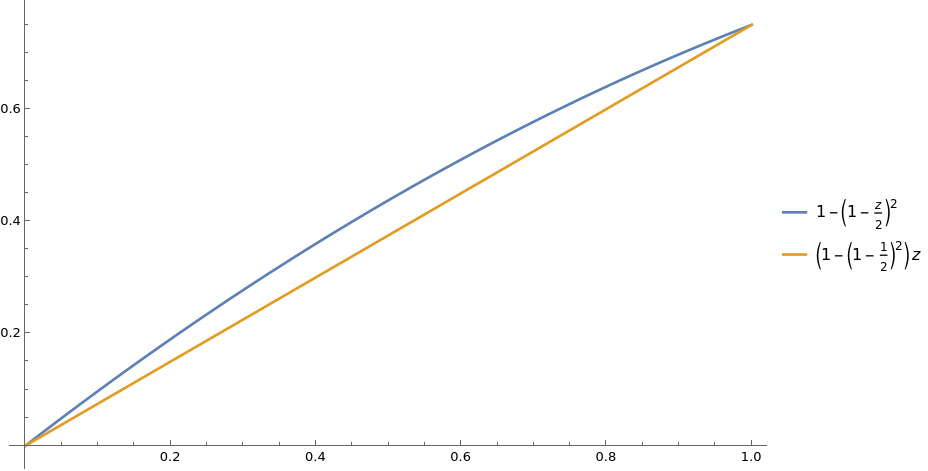
\includegraphics[width=1.25\textwidth]{figures/fig-randomrounding-concaveconcave.png}
        \caption{An illustration of the inequality for $\ell=2$.}
        \label{fig:randomrounding:concave}
    \end{figure}
    Using this, we finally get\marginnote{We invoke the ``fact'' that 
    \[
    \sup_{\ell \geq 1}\Paren{ 1-\frac{1}{\ell_j}}^{\ell_j} = 1/e\,.
    \]
    }
        \begin{align}
        \expect{\val_\phi(x)} 
        &\geq \sum_{j=1}^{\green{m}} \Paren{1-\Paren{ 1-\frac{1}{\ell_j}}^{\ell_j}}\cdot z^\ast_j \label{eq:intermediate:rounding:guarantee}\\
        &\geq \inf_{\ell \geq 1}\Paren{1-\Paren{ 1-\frac{1}{\ell}}^{\ell}}  \cdot \sum_{j=1}^{\green{m}} z^\ast_j \notag\\
        &= \Paren{1-\frac{1}{e}} \opt_{\rm LP} \notag\\
        &\geq \Paren{1-\frac{1}{e}} \opt_{\rm ILP} \notag
    \end{align}
    concluding the proof.
\end{proof}

\paragraph{Are we done?} We started by showing a simple randomised approach giving an expected $1/2$-approximation to \textsc{Max-SAT}. By spending more time, effort, and relaxing (an ILP), we obtained an efficient randomised algorithm, less simple but giving a better guarantee: an expected $0.632$-approximation. \emph{Can we do better?}

Surprisingly, yes: we can get a $3/4$-approximation, by combining the two! This is quite unexpected, as combining two algorithms will give a better result than \emph{both}. The crucial insight is that, as remarked before, the naive randomised approach fares very well on \emph{long} clauses. What about the LP-relaxation one? Roughly speaking, its expected approximation guarantee on a clause of length $\ell_j$ is
\[
\Paren{1-\Paren{ 1-\frac{1}{\ell_j}}^{\ell_j}}
\]
\emph{which is better for short clauses}! (As you can see, for $\ell_j = 1$ this takes value $1$, for $\ell_j=2$ it is $3/4$\dots We may hope that choosing the best of the two solutions (one better when clauses are typically long, the other better when they are typically short) could be beneficial. 
\begin{theorem}
    \label{theo:randomised:maxsat:bestoftwo}
    The ``best-of-two'' approach which runs both the naive randomised algorithm of~\cref{theo:randomised:maxsat} and the randomised rounding of~\cref{theo:randomrounding:maxsat} gives, in expectation, a $3/4$-approximation for \textsc{Max-SAT}.
\end{theorem}
\begin{proof}
    The proof is quite simple: denote by $x,x'$ the two solutions returned. Then, since the $\max$ is at least the average,
    \begin{align*}
        \expect{\max\Paren{\val_\phi(x),\val_\phi(x')}} 
        &\geq \frac{1}{2}\expect{\val_\phi(x)+\val_\phi(x')} \\
        &\geq \frac{1}{2}\sum_{j=1}^{\green{m}}\Paren{ \Paren{1-\frac{1}{2^{\ell_j}}} +  \Paren{1-\Paren{ 1-\frac{1}{\ell_j}}^{\ell_j}}\cdot z^\ast_j } 
         \tag{By~\eqref{eq:intermediate:naiverandomised} and~\eqref{eq:intermediate:rounding:guarantee}} \\
        &\geq \frac{1}{2}\sum_{j=1}^{\green{m}}\Paren{ \Paren{1-\frac{1}{2^{\ell_j}}} +  \Paren{1-\Paren{ 1-\frac{1}{\ell_j}}^{\ell_j}} } \cdot z^\ast_j
         \tag{as $z^\ast_j \leq 1$}\\
         &\geq \frac{3}{4}\sum_{j=1}^{\green{m}}z^\ast_j
         \tag{$\star$}\\
         &\geq \frac{3}{4}\opt_{\rm ILP}
    \end{align*}
    where the inequality $(\star)$ follows from the (somewhat technical) claim that, for every $x\geq 2$ \emph{and} for $x=1$, we have (see~\cref{fig:randomrounding:bestofboth})
    \[
    \Paren{1-\frac{1}{2^{x}}} +  \Paren{1-\Paren{ 1-\frac{1}{x}}^{x}} \geq \frac{3}{2}\,.
    \]
    This concludes the proof, and the chapter.
\end{proof}
    \begin{figure}[htbp]
        \centering
        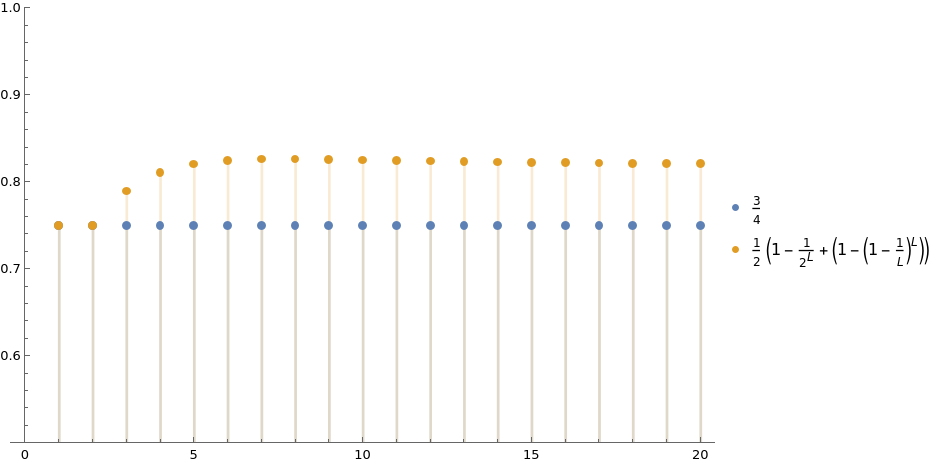
\includegraphics[width=1.25\textwidth]{figures/fig-randomrounding-bestofboth.png}
        \caption{An illustration of the last, ``magical'' inequality. Note that it does not hold for values in $(1,2)$, but, thankfully, we only need it for integers.}
        \label{fig:randomrounding:bestofboth}
    \end{figure}

\chapter{Lecture 11: Learning and testing probability distributions}
In all we have done so far in this unit, we have assumed that the input was deterministic: the algorithm is randomised, yes, but the input itself is fixed, and arbitrary.

In this lecture, we (somewhat) change this. What we have is access to a sequence of independent, identically distributed (\iid) data points, coming from an \emph{unknown} probability distribution $\p$:
\[
    x_1,\dots, x_\ns \sim \p
\]
and what we want to do is to \emph{learn something about this $\p$}. Put differently:
\begin{framed}
    \noindent The input is not the \iid sequence $(x_1,\dots, x_\ns)$: the input is $\p$, and  $x_1,\dots, x_\ns$ is how we get to access this input.
\end{framed}
We will make very few assumptions about this unknown probability distribution $\p$: except that it is over a known \emph{discrete} domain $\domain$ of size $\abs{\domain} = \ab$. 

To illustrate this, here is a histogram, corresponding to the counts from $\ns=3665$ \iid\ draws\marginnote{\emph{Presumably} \iid} from some unknown probability distribution $\p$ over $\domain = \{1,2,\dots,49\}$ of size $\ab=49$. They correspond to a number drawn, every week from 1982 to 2018, from Canada's ``Lotto 6/49'':
\begin{figure}[htbp]
    \centering
    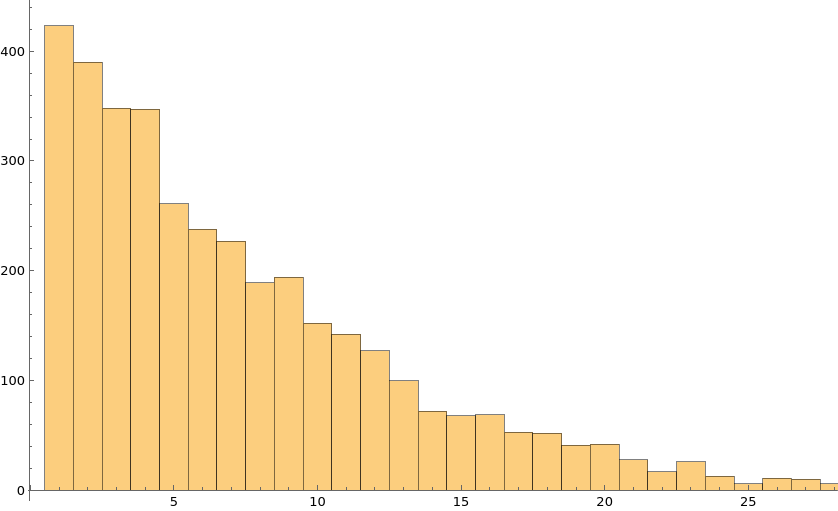
\includegraphics[width=0.925\linewidth]{figures/fig-lotto-minofsix.png}
    \caption{Counts for each of the $\ab=49$ possible numbers among the $\ns=3665$ draws. What is distribution $\p$ does this correspond to? (Data from the Kaggle ``Lotto 649'' dataset.)}
    \label{fig:enter-label} % Min of 6 uniform
\end{figure}
\noindent Here are some questions we may want to answer about $\p$:
\begin{itemize}
    \item \emph{What is it?} That is, can we \emph{learn} the whole unknown probability distribution?
    \item \emph{What are some of its characteristics?} That is, can we \emph{learn} some ``simple'' parameter $f(\p)$, such as its mean, entropy, variance?
    \item \emph{Does it satisfy some specific property?} That is, can we \emph{test} if $\p$ satisfies some requirement we care about? For instance, in the case of the lotto numbers above, ``{is $\p$ consistent with the distribution of the minimum of 6 independent uniform random numbers in $\{1,2,\dots, 49\}$?}''
\end{itemize}
Intuitively, we can think of the first as learning $\approx \ab$ values about $\p$, the second as learning \emph{one} value, and the last one as learning \emph{one bit}. So presumably, they should be in decreasing order of ``complexity,'' for whatever notion of ``complexity'' we define.


\paragraph{What is the notion of complexity?} Our algorithms, as mentioned about, can only access the input $\p$ through queries which give\marginnote{Think of $\ns$ as the size of the dataset you need to collect, or generate, or buy in order for your algorithm to succeed. In the case of the lotto example, the number of observations is limited: there is only one lotto every week, we cannot choose $\ns$ to be as large as we want.} \emph{independent, identically distributed} samples from $\p$. We will of course care about the running time of the algorithms, but our main objective  will be to minimise the number $\ns$ of queries we make.

\paragraph{What is the randomness?} Since what we feed to the algorithm, the sequence of samples $x_1,\dots, x_\ns$, is random, there will always be some probability our algorithm's output is wrong. That is, now, when we discuss expectations and probabilities, it will be over (1)~the randomness of the algorithm itself, as usual, but also (2)~the randomness in drawing $x_1,\dots, x_\ns$ from the unknown $\p$.

\paragraph{What are the parameters?} Of course, the domain size, $\ab$, is a key 
parameter of the problem. But we have at least two others: first, the probability of failure, $\errprob$: we want the algorithm to be correct about $\p$ most of the time. The other will be a \emph{distance parameter}, $\dst >0$: we will get back to this soon, as its meaning depends on which of the three problems we are interested in. But overall, our goal will be:
\begin{framed}
    Find the smallest value $\ns = \ns(\ab, \dst, \errprob)$ for which an algorithm can solve the learning, estimation, or testing task we care about with distance parameter $\dst$ and failure probability at most $\errprob$. 
\end{framed}

\paragraph{Some notation} A probability distribution over $\domain$ can be identified to its probability mass function (pmf), which is a function $\p\colon\domain\to [0,1]$ such that $\sum_{x\in \domain}\p(x) = 1$. Accordingly, the probability mass that $\p$ assigns to a subset\footnote{As we only consider discrete domains, we ignore issues of measurability, etc. That is, we consider $\domain$ endowed with the counting measure, so every set is measurable. What is discussed here generalises to continuous probability distributions, but with annoying technical details.} $S\subseteq \domain$ is $\p(S) = \sum_{x\in S} \p(x) = \probaDistrOf{x\sim\p}{x\in S}$. Finally, $\distribs{\domain}$ denotes the set of all probability distributions over our domain $\domain$.

\section{Distance between probability distributions}
To define what it means to learn a probability distribution, or even how \emph{far} two probability distributions over the same domain $\domain$ are, we need a notion of \emph{distance}. Ideally, one which makes ``sense'': (1)~a metric would be nice (to be able to use the triangle inequality when needed), (2)~a \emph{bounded} metric would be even nicer (to be able to understand a value such as $0.1$ without having to normalise or think twice), (3)~a bounded metric \emph{with a simple and meaningful interpretation} would be best.

This leads us to the the notion of distance we will be concerned about, the total variation distance (also known as \emph{statistical distance}).
\begin{definition}[Total variation distance]
  \label{def:tv}
  The \emph{total variation distance} between two probability distributions $\p,\q\in\distribs{\domain}$ is given by
  \[
    \totalvardist{\p}{\q} = \sup_{S\subseteq \domain} (\p(S)-\q(S))\,.
  \]
  Given a subset $\class\subseteq\distribs{\domain}$ of distributions, we further define the distance from $\p\in\distribs{\domain}$ to $\class$ as $\totalvardist{\p}{\class} \eqdef \inf_{\q\in\class} \totalvardist{\p}{\q}$, and will say that $\p$ is \emph{$\dst$-far from $\class$} if $\totalvardist{\p}{\class} > \dst$.
\end{definition}
One can check\marginnote{Check it!} that $\dtv$ defines a metric on $\distribs{\domain}$, and takes values in $[0,1]$. Moreover, the total variation distance exhibits several important properties, among which one of the most important is its \emph{immunity to post-processing}:
\begin{fact}[Data Processing Inequality]
  \label{fact:dpi}
  Suppose $X$ and $Y$ are independent random variables with distributions $\p$ and $\q$, and let $f$ be any (possibly randomized) function independent of $X,Y$. Then the probability distributions $\p_f$ and $\q_f$ of $f(X)$ and $f(Y)$ satisfy
  \[
      \totalvardist{\p_f}{\q_f} \leq \totalvardist{\p}{\q}\,.
  \]
  That is, \emph{postprocessing cannot increase the total variation distance.}
\end{fact}
What this says is, paraphrasing, that post-processing two random variables the same way cannot ``make them statistically farther.''


%%%%%%%%%%%%%%%%%%%%%%%%%%%
Interestingly, total variation distance also has a very natural interpretation in terms of \emph{indistinguishability}:
\begin{lemma}[Pearson--Neyman]
  \label{lemma:pearsonneyman}
  Any (possibly randomized) algorithm which distinguishes between $\p$ and $\q$ from a \emph{single} sample must have Type~I (false positive) and Type-II (false negative) errors satisfying
  \[
      \text{Type~I} + \text{Type~II} \geq 1- \totalvardist{\p}{\q}
  \]
  Moreover, this is achieved by the test which outputs ``$\q$'' if, and only if, the sample belongs to the ``Scheff\'e set'' $S^\ast \eqdef \setOfSuchThat{x}{\q(x) > \p(x)}$.
\end{lemma}
\begin{proof}\marginnote{You can ignore the proof in a first read, it is just here for completeness. What matters is the lemma itself.}
Fix any test $\Algo$ distinguishing between two distributions $\p$ and $\q$, given a single observation. Letting $\alpha$ and $\beta$ denote the Type~I and Type-II errors of $\Algo$, we have
\begin{align*}
  \alpha+\beta 
  &= \probaDistrOf{\p,R}{\Algo(X,R)=1} + \probaDistrOf{\q,R}{\Algo(X,R)=0} \\
  &= \shortexpect_{R}[ \probaDistrOf{\p}{\Algo(X,R)=1} ] + \shortexpect_{R}[ \probaDistrOf{\q}{\Algo(X,R)=0} ] \\
  &= \shortexpect_{R}[ \probaDistrOf{\p}{\Algo(X,R)=1} + \probaDistrOf{\q}{\Algo(X,R)=0} ]
%   \totalvardist{\p}{\q}
\end{align*}
where we denote by $R$ the internal randomness of $\Algo$. Since, for any fixed realization $r$ of this randomness $R$, the resulting test $\Algo(\cdot,r)$ is deterministic, we can define for any $r$ the \emph{acceptance region} $S_{\Algo,r} \eqdef \setOfSuchThat{x}{\Algo(x,r)=1}$, and write
\begin{align*}
  \alpha+\beta 
  &= \shortexpect_{R}[ \probaDistrOf{\p}{X \in S_{\Algo,R}} + \probaDistrOf{\q}{X \notin S_{\Algo,R}} ] \\
  &= 1+\shortexpect_{R}[ \p(S_{\Algo,R}) - \q(S_{\Algo,R}) ] \\
  &\geq 1 + \inf_{S}(\p(S) - \q(S)) \\
  &= 1 - \sup_{S}(\q(S) - \p(S)) \\
  &= 1- \totalvardist{\p}{\q}\,,
\end{align*}
as claimed. Finally, it is immediate from the definition of total variation distance that the proposed test satisfies $\text{Type~I} + \text{Type~II} = 1 + \p(S^\ast) - \q(S^\ast) = 1- \totalvardist{\p}{\q}$.
\end{proof}
%%%%%%%%%%%%%%%%%%%%%%%%%%%
Here is one way to interpret this lemma: 
\begin{framed}
Alice and Bob play a game, where they both know two probability distributions $\p,\q$. Alice starts by tossing a fair coin, and does not show the outcome to Bob: if it is \textsf{Heads}, then she draws $x\sim \p$; if it is \textsf{Tails}, she draws $x\sim \q$. Then she shows the value of $x$ to Bob, who must guess if the coin toss was \textsf{Heads}.
Clearly, just by random guessing, Bob can win the game with probability $1/2$. What the lemma says is that he can do better: there is a strategy for him to win with probability
\[
    \probaOf{\text{Bob wins}} = \frac{1}{2}+\frac{\totalvardist{\p}{\q}}{2}
\]
and, moreover, this is the best possible.
\end{framed}
One more (very useful) fact about total variation distance: it is just $\lp[1]$ distance in disguise!
\begin{fact}[Scheff\'e's Lemma]
\label{fact:scheffe}
For any two $\p,\q\in\distribs{\ab}$,
  \begin{equation}
    \label{eq:tv:l1}
    \totalvardist{\p}{\q} = \frac{1}{2}\sum_{x\in\domain} \abs{\p(x)-\q(x)} = \frac{1}{2}\normone{\p-\q}
  \end{equation}
  that is, ``total variation is half the $\lp[1]$ distance between pmfs.''
\end{fact}
This fact, which you will prove during the tutorial, turns out to be a very useful connection: if nothing else, $\lp[p]$ norms are well studied, and this will allow us to use our arsenal of geometric inequalities --- H\"older, Cauchy--Schwarz, and monotonicity of $\lp[p]$ norms, to name a few.

\section{The case of a coin ($\ab=2$)}
With the necessary background in hand, we can look at our first question: forget for now about $\ab \gg 1$, let us focus on the simplest, most basic case, $\ab=2$: you are given \emph{a coin}, and it may be biased.

The learning task can be then rephrased as follows:
\begin{framed}
    How many times $\ns$ do you need to flip the coin to learn its true bias $p$ to accuracy $\pm\dst$, and be correct with probability at least $1-\errprob$?
\end{framed}
\noindent Should it be\dots
\begin{itemize}
    \item $\ns = \bigO{\frac{1}{\dst\errprob}}$ times?
    \item $\ns = \bigO{\frac{1}{\dst^2\errprob}}$ times?
    \item $\ns = \bigO{\frac{1}{\dst^2}\log\frac{1}{\errprob}}$ times?
    \item $\ns = \bigO{\frac{1}{\dst}\log\frac{1}{\errprob}}$ times?
\end{itemize}
Well, actually, we can get something more refined than any of the bounds above! If we are given a promise on the unknown bias $p$, then we can get the following:
\begin{theorem}
    Suppose we are promised that the true bias $p$ of the coin satisfies $0\leq p < q \leq \frac{1}{2}$, for some known value $q$. Then estimating the bias of the coin to an additive $\dst$, with probability at least $1-\errprob$, can be done with $\ns = \bigO{\frac{q}{\dst^2}\log\frac{1}{\errprob}}$ \iid samples. (Moreover, this is optimal.)
\end{theorem}
\begin{proof}
    This follows from a Chernoff bound, using the empirical estimate
    \[
        \hat{p} \eqdef \frac{1}{\ns}\sum_{i=1}^\ns x_i
    \]
    where $x_1, \dots, x_\ns \sim \bernoulli{p}$.
    Note that a Hoeffding bound would not give you the dependence on $q$. (The lower bound, \ie proof of optimality, is beyond the scope of this lecture.)
\end{proof}
As a remark, the assumption that $q \in(0,1/2]$ is without loss of generality: if instead we were promised that $q < p \leq 1$ with $q \in (1/2, 1)$, then we could flip the coin flips (!) by looking at $x'_i \eqdef 1-x_i$ instead, and estimate the bias $p' \eqdef 1-p$, which satisfies $0 \leq p' < 1-q \leq 1/2$. Clearly, estimating $p'$ to $\pm\dst$ is equivalent to estimate $p$ to $\pm \dst$.
\begin{corollary}
    \label{theo:learning:bias}
    Estimating the bias of a coin to an additive $\dst$, with probability at least $1-\errprob$, can be done with $\ns = \bigO{\frac{1}{\dst^2}\log\frac{1}{\errprob}}$ \iid samples. (Moreover, this is optimal.)
\end{corollary}
This follows from applying the above theorem setting $q=1/2$; alternatively, the upper bound can be directly proven using the Hoeffding bound.\marginnote{Try it!}

This is if we want to \emph{learn} the bias of an unknown coin. What if we just want to \emph{test} if it is biased? That is, distinguish between the case where (1)~the coin is \textsf{Heads} with probability exactly $1/2$ (fair coin), or probability $1/2 \pm \Omega(\dst)$ (biased coin)? How many times $\ns$ would we have to toss the coin, if we wanted our diagnostic to be correct with probability at least $1-\errprob$?
\begin{itemize}
    \item $\ns = \bigO{\frac{1}{\dst}\sqrt{\log\frac{1}{\errprob}}}$ times?
    \item $\ns = \bigO{\frac{1}{\dst^2}\sqrt{\log\frac{1}{\errprob}}}$ times?
    \item $\ns = \bigO{\frac{1}{\dst^2}\log\frac{1}{\errprob}}$ times?
    \item $\ns = \bigO{\frac{1}{\dst}\log\frac{1}{\errprob}}$ times?
\end{itemize}
As it turns out\dots \emph{testing} whether the coin is biased or fair is basically as hard as \emph{learning} the bias of the coin:
\begin{theorem}
    \label{theo:testing:bias:basic}
    Testing whether the bias of a coin is $1/2$ or at least $1/2+\dst$, with probability at least $1-\errprob$, can be done with $\ns = \bigO{\frac{1}{\dst^2}\log\frac{1}{\errprob}}$ \iid samples. (Moreover, this is optimal.)
\end{theorem}
This is a little underwhelming, since one can literally do this by learning the bias up to $\frac{\dst}{2}$.\footnote{Can you see how?} And that provides a lot more information! So is there anything to be gained (except maybe constant factors) if we only want to test tthe bias of the coin? As it turns out, \emph{yes}\dots but not always. \emph{Not} when testing if a coin is fair or biased: but when testing if the coin is very biased or \emph{extremely} biased, then yes.
\begin{theorem}
\label{theo:testing:bias:refined}
    For any $0 <\purple{\alpha} \leq 1/2$ and $\dst\in(0,1]$, testing whether the bias of a coin is at most $\purple{\alpha}$ or at least $\purple{\alpha}(1+\dst)$, with probability at least $1-\errprob$, can be done with $\ns = \bigO{\frac{1}{\purple{\alpha}\dst^2}\log\frac{1}{\errprob}}$ \iid samples.
\end{theorem}
Again, this is not very useful when $\purple{\alpha} = \Omega(1)$: however, for vanishing $\purple{\alpha}$, this is much better than what learning the bias to an additive $\pm \frac{1}{2}\purple{\alpha}\dst$ would give, which by~\cref{theo:learning:bias} is $\ns= \bigO{\frac{1}{\purple{\alpha}^2\dst^2}\log\frac{1}{\errprob}}$.

\cref{theo:testing:bias:refined} can be proven by a Chernoff bound, specifically the version given in~\cref{theo:chernoff:with:ublb} applied to the same empirical estimator $\hat{p}$. But rather than \emph{proving} it, let us give a small sketch of \emph{why} we could expect this statement to be true, to get some intuition (and remember the result). If the true bias $p$ is roughly $\Theta(\purple{\alpha})$, then we expect to see \textsf{Tails} most of the time, and \textsf{Heads} a $\Theta(\purple{\alpha})$ fraction of the tosses. That is, in every chunk of $1/\purple{2\alpha}$ tosses, we expect to see a \textsf{Heads} with probability either at most $1/2$ (if $p \leq \purple{\alpha}$) or at least $(1+\dst)/2$ (if $p \geq (1+\dst)\purple{\alpha}$). But by~\cref{theo:testing:bias:basic} (ignoring $\errprob$ for simplicity), this takes $\bigO{{1}/{\dst^2}}$ chunks~--~so $\bigO{{1}/{(\purple{\alpha}\dst^2)}}$ coin tosses in total.

\emph{And this makes sense!} Things should become easier in the ``highly biased'' regime. With a similar analysis, one can show that distinguishing between bias $p=0$ and bias $p\geq \dst$ takes only $\ns=O(1/\dst \log(1/\errprob))$ coin tosses. And this is easy to interpret: in one case, you \emph{never} see a \textsf{Heads}, and in the other, you will see one after $\approx 1/\dst$ coin tosses. What is really hard (and requires more coin tosses) is when $p\approx 1/2$, and you have to distinguish between ``a lot of \textsf{Heads}'' and ``a lot of \textsf{Heads}, \emph{but slightly more}.''

\section{Learning and testing beyond coins}
This is all well and good, but we often have to consider data over domains of size $\ab \gg 2$. The lotto example above, for instance, was for $\ab = 49$; and that's only for \emph{one} number: if one considers all 6 draws in a single ticket of that Canadian lotto, that's a domain of size $\ab = 49^6 = 13,841,287,201$.

If we were given an algorithm to generate random permutations and we wanted to test whether its output was truly uniform (on the space of all permutations of, say, size $8$), then we would be looking at a space of size $16! = 209,22,789,888,000$.

If we wanted to estimate the entropy of a dataset of $8$-character passwords made of lower and uppercase letters, digits, and special characters $\$\%\#\&!?\_-$, then $\ab = (70)^{8} = 576,480,100,000,000$. 
\begin{framed}
Domain sizes grow quite fast, and in most settings $\ab$ is huge.
\end{framed}
If we cannot assume structure in the data, then we have to hope for \emph{very} sample-efficient algorithms.

\section{Learning}
In \emph{learning} (in total variation distance),\footnote{One can define learning with respect to other notions of distances: \eg Kullback--Leibler divergence, or $\lp[\infty]$ distance. Here we focus on the standard, nice, total variation.} our goal is to design an algorithm $\Algo$ which, given $\ns$ \iid samples from $\p$ and parameters $\dst,\errprob\in(0,1]$, outputs $\widehat{\p}$ such that
\begin{equation}
    \probaOf{ \totalvardist{\p}{\widehat{\p}} > \dst } \leq \errprob
\end{equation}
that is, $\widehat{\p}$ is close to $\p$, with high probability. The probability is taken, again, over both the samples $x_1,\dots, x_{\ns}\sim \p$ \emph{and} the randomness of the algorithm $\Algo$.

How many samples $\ns$ would we have to take, if we wanted the output $\widehat{\p}$ to be $\dst$-close to the true $\p$ with probability at least $1-\errprob$?
\begin{itemize}
    \item $\ns = \bigO{\frac{\ab^2}{\dst}\log\frac{1}{\errprob}}$?
    \item $\ns = \bigO{\frac{\ab}{\dst^2}\log\frac{1}{\errprob}}$?
    \item $\ns = \bigO{\frac{\ab + \log\frac{1}{\errprob}}{\dst^2}}$?
    \item $\ns = \bigO{\frac{\ab^2 + \log\frac{1}{\errprob}}{\dst^2}}$?
\end{itemize}
As we will see, the answer is not entirely obvious, even though the algorithm $\Algo$ is. 

\paragraph{First idea: using what we saw}
We want to estimate all $\ab$ probabilities $\p_1,\dots, \p_{\ab}$ to get $\widehat{\p}_1,\dots,\widehat{\p}_{\ab}$ such that
\[
    \frac{1}{2}\sum_{i=1}^{\ab} \abs{\widehat{\p}_i-\p_i} \leq \dst\,.
\]
It would be \emph{enough} to estimate each individual $\p_i$ to an additive $\frac{2\dst}{\ab}$.\footnote{Ignore for now the fact that doing so, we may not have $\sum_{i=1}^{\ab} \widehat{\p}_i = 1$: we can normalise afterwards.} To make sure we learn \emph{all} $\ab$ of them, we will learn each with error failure $\frac{\errprob}{\ab}$ and take a union bound.

The total cost, from~\cref{theo:learning:bias}, is then
\begin{equation}
\ns = \bigO{ \frac{1}{(\dst/\ab)^2} \log\frac{1}{(\errprob/\ab)} }
= \bigO{ \frac{\ab^2}{\dst^2}\log\frac{\ab}{\errprob} }\,.
\end{equation}
That's something, but that has a more-than-\emph{quadratic} dependence on this giant parameter $\ab$. \smallskip

\emph{But we can do better!} Another idea would be to learn each $\p_i$ to a multiplicative factor $(1\pm 2\dst)$, instead of an additive $\pm \frac{2\dst}{\ab}$. \emph{If} we assume that $\p_i \geq \frac{\dst}{\ab}$ for all $1\leq i\leq \ab$, for instance, then a Chernoff bound (along with a union bound) tell us that we can the empirical estimates $\hat{\p}_1,$ satisfy
\[
    (1- 2\dst)\p_i \leq \widehat{\p}_i \leq (1+2\dst)\p_i, \text{ for all } 1\leq i\leq \ab
\]
with probability at least $1-\errprob$, for
\begin{equation}
    \ns = \bigO{ \frac{\ab}{\dst^3}\log\frac{\ab}{\errprob} }
\end{equation}
and then
\[
    \frac{1}{2}\sum_{i=1}^{\ab} \abs{\widehat{\p}_i-\p_i} \leq \frac{1}{2}\sum_{i=1}^{\ab} 2\dst \p_i = \dst\,,
\]
since $\sum_{i=1}^{\ab} \p_i = 1$. Moreover, we can get rid of that assumption on $\min_i \p_i$, losing only constant factors in the final bound.\marginnote{$(\star)$ Can you see how? Hint: ``mix'' $\p$ with uniform, and learn \[
\p' = (1-\frac{\dst}{2})\p + \frac{\dst}{2}\uniform_{\ab}
\]instead, where $\uniform_{\ab}$ is the uniform distribution on $\domain$.}\medskip

\emph{But we can do better!} One of the two bounds above has a (near) quadratic dependence on $\ab$ but a quadratic dependence on $1/\dst$, the other is (near) linear in $\ab$ but has a cubic dependence on $1/\dst$, and both have an extra logarithmic factor in $\ab$ because of a union bound. This does not ``feel'' right, and indeed it is not:

\begin{theorem}
    \label{theo:learning:k}
    Learning an unknown distribution $\p\in\distribs{\ab}$ to total variation distance $\dst$ (with success probability $1-\errprob$) can be done with 
    \[
    \ns = \bigO{\frac{\ab + \log\frac{1}{\errprob}}{\dst^2}}
    \]\iid samples. (Moreover, this is optimal.)
\end{theorem}
% Talk about monotonicity in the tutorial?
% DKW?
We will only prove the upper bound statement (not the lower bound showing this sample complexity is optimal), but it is worth noting that we have $\ab+\log(1/\errprob)$, \emph{not} $\ab\log(1/\errprob)$: this is perhaps surprising, as $\ab\log(1/\errprob)$ is what the median trick would give us.
\begin{proof}[Proof of~\cref{theo:learning:k}]
    Consider the empirical distribution $\widehat{\p}$ obtained by drawing $\ns$ independent samples $x_1,\dots,x_\ns$ from the underlying distribution $\p\in\distribs{[\ab]}$:
\begin{equation}\label{def:empirical}
\widehat{\p}(i) = \frac{1}{\ns} \sum_{j=1}^\ns \indic{x_j=i}, \qquad i\in [\ab]
\end{equation}
This defines a valid probability distribution (\ie $\widehat{\p}\in\distribs{\ab}$), and moreover can be computed efficiently, in time $O(\ab+\ns\log\ns)$.

Recalling the definition of total variation distance (\cref{def:tv}), the key observation is that we have $\totalvardist{\p}{\widehat{\p}} > \dst$ if, and only if, there exists a subset $S\subseteq [\ab]$ such that $\widehat{\p}(S) > \p(S) + \dst$. There are only $2^{\ab}$ subsets (actually $2^{\ab}-2$) to consider, so we will make sure our estimate is accurate for \emph{each} subset, taking a union bound over all $2^{\ab}$ of them.

Fix any $S\subseteq[\ab]$. We have
\[
	\widehat{\p}(S) = \sum_{i\in S} \widehat{\p}(i) \operatorname*{=}^{\eqref{def:empirical}} \frac{1}{\ns} \sum_{i\in S} \sum_{j=1}^\ns \indic{x_j=i}
\]
and so, letting $X_j \eqdef \sum_{i\in S}\indic{x_j=i}$ for $j\in [\ns]$, we have
$
\widehat{\p}(S) = \frac{1}{\ns}\sum_{j=1}^\ns X_j
$ where the $X_j$'s are \iid Bernoulli random variables with parameter $\p(S)$. By a Hoeffding bound,
\[
    \probaOf{ \widehat{\p}(S) > \p(S) + \dst } = \probaOf{ \frac{1}{\ns}\sum_{j=1}^\ns X_j > \expect{\frac{1}{\ns}\sum_{j=1}^\ns X_j} + \dst } \leq e^{-2\dst^2 \ns}
\]
and therefore $\probaOf{ \widehat{\p}(S) > \p(S) + \dst } \leq \frac{\errprob}{2^{\ab}}$ as long as
\begin{equation}
\ns\geq \frac{\ab\ln 2+\log(1/\errprob)}{2\dst^2}
\end{equation}
A union bound over these $2^{\ab}$ possible sets $S$ concludes the proof:
\[
    \probaOf{ \exists S\subseteq [\ab] \text{ s.t. }\widehat{\p}(S) > \p(S) + \dst } \leq 2^{\ab}\cdot \frac{\errprob}{2^{\ab}} = \errprob\,.\qedhere
\]
\end{proof}
This proof is a little magical, and crucially relies on the definition of total variation distance as a supremum over subsets. One can also prove the statement using the equivalent characterisation (from~\cref{fact:scheffe}) as $\lp[1]$ distance. We will only prove it for constant $\errprob$, as the full version requires a tool (McDiarmid's inequality) we have not seen in this class.
\begin{proof}[Alternative proof of~\cref{theo:learning:k}]
Consider the empirical distribution $\widehat{\p}$ from $\ns$ \iid samples defined in~\eqref{def:empirical}. 

First, we bound the \emph{expected} total variation distance between $\widehat{\p}$ and $\p$, by using $\lp[2]$ distance as a proxy:
\begin{align*}
    \expect{ \totalvardist{\p}{\widehat{\p}} }
    &=\frac{1}{2}\expect{ \normone{\p-\widehat{\p}}} 
    =\frac{1}{2}\sum_{i=1}^{\ab}\expect{ \abs{\p(i)-\widehat{\p}(i)}} \\
    &\leq\frac{1}{2}\sum_{i=1}^{\ab}\sqrt{\expect{ (\p(i)-\widehat{\p}(i))^2} }
\end{align*}
the last inequality by Jensen. But since, for every $i\in[\ab]$, $\ns\widehat{\p}(i)$ follows a $\binomial{\ns}{\p(i)}$ distribution, we have
\[
\expect{ (\p(i)-\widehat{\p}(i))^2} = \frac{1}{\ns^2}\var[\ns\widehat{\p}(i)] = \frac{1}{\ns}\p(i)(1-\p(i))
\]from which
\[
    \expect{ \totalvardist{\p}{\widehat{\p}} } \leq\frac{1}{2\sqrt{\ns}}\sum_{i=1}^{\ab}\sqrt{\p(i)} \leq \frac{1}{2}\sqrt{\frac{\ab}{\ns}}
\]
the last inequality this time by Cauchy--Schwarz. Therefore, for $\ns\geq \frac{25\ab}{\dst^2}$ we have $\expect{ \totalvardist{\p}{\widehat{\p}} }\leq \frac{\dst}{10}$.

We can then conclude by Markov's inequality, establishing that
\[
    \probaOf{  \totalvardist{\p}{\widehat{\p}} \geq \dst } \leq \frac{1}{10}\,.\qedhere
\]
\end{proof}
$(\star)$ A final (and side) remark: this last proof actually establishes a slightly stronger result, namely, that the sample complexity $\ns$ can be expressed as
$
\ns = \bigO{{\norm{\p}_{1/2}}/{\dst^2}}
$, 
where $\norm{\p}_{1/2} = \Paren{\sum_{i=1}^{\ab} \sqrt{\p(i)}}^2$ is the ``$\frac{1}{2}$-norm'' of the unknown distribution $\p$.\marginnote{This is (1)~not examinable, and (2)~not a norm.}
\section{Testing}
As we just saw, we can learn the \emph{whole} probability distribution $\p$ to accuracy $\dst$ using $O(\ab/\dst^2)$ samples. What if we only wanted to test if $\p$ had some important property? For instance, if $\p=\q$, where $\q\in\distribs{\ab}$ is some known reference distribution?

Specifically, we want to solve the following problem: \marginnote{This question is called ``identity testing'' in the distribution testing literature.}
\begin{framed}
    Give an algorithm $\Algo$ which takes parameters $\dst,\errprob\in(0,1]$ and $\ns$ samples from $\p$, and:
\begin{itemize}
    \item If $\p=\q$, then $\probaOf{\Algo \text{ outputs } \yes} \geq 1-\errprob$;
    \item If $\totalvardist{\p}{\q} > \dst$, then $\probaOf{\Algo \text{ outputs } \no} \geq 1-\errprob$
\end{itemize}
(if $0 < \totalvardist{\p}{\q} \leq \dst$, then $\Algo$ is off the hook and can output whatever).
\end{framed}
\emph{Why do we care?} For instance, someone may hand you an algorithm claiming it samples a uniformly random permutation; or the implementation of a hash family $\green{\mathcal{H}}$, claiming its output $h(x)$ (over the choice of $h\sim\green{\mathcal{H}}$) is uniformly distributed for each $x$; or you may have an algorithm running really well on uniformly random data, but very poorly on very skewed data~--~and you want to test these claims, or if your dataset is uniform enough for your fast algorithm.

\begin{figure}[htbp]\centering
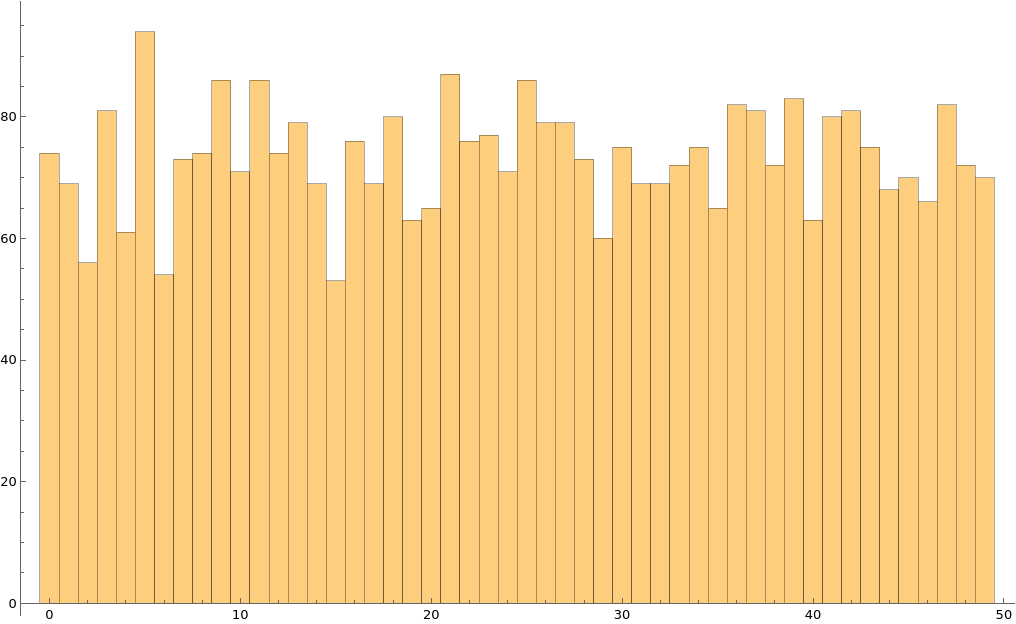
\includegraphics[width=0.75\textwidth]{figures/fig-lotto-bonusnumberuniform}
\caption{Histogram of 3,665 draws of the ``bonus number'' in Canada's 6/49 lotto, each draw being a number in $\{1,2,\dots,49\}$. Is the distribution uniform? Or is the lottery not fair?}
\end{figure}

So you have a reference distribution $\q\in\distribs{\ab}$ in mind. The first thing we will do is simplify the problem, and assume that $\q$ is not \emph{any} distribution, but \emph{the} uniform distribution $\uniformOn{\ab}$ over $\domain$.\marginnote{This is the \emph{uniformity testing} question, a special case of identity testing.} This will make our life easier. And while this seems like a big simplification, it turns out it is not! That is, any algorithm for \emph{uniformity testing} (the reference is $\uniformOn{\ab}$) can be used as a blackbox to solve the \emph{identity testing} (the reference is any $\q$), \emph{via} a reduction:
\begin{theorem}[Identity to uniformity reduction]
Suppose there is an algorithm $\Algo$ for uniformity testing, which takes $\ns=\ns(\ab,\dst,\errprob)$ \iid samples from the unknown distribution. Then there is an algorithm $\Algo'$ for identity testing over a domain of size $\ab$ to any fixed $\q\in\distribs{\ab}$, which takes $\ns=\ns(4\ab,\dst/4,\errprob)$ \iid samples from the unknown distribution. Moreover, $\Algo'$ is efficient if $\Algo$ is.
\end{theorem}
We will not prove this theorem here, but this essentially says that while uniformity and identity testing, they are basically equivalent (up to constant factors).

Now, all we need to solve is the \emph{uniformity testing} problem: given $\ns$ \iid samples from an unknown $\p$ over $\domain$, decide whether $\p=\uniformOn{\ab}$, or $\totalvardist{\p}{\uniformOn{\ab}} > \dst$ (and be correct with probability at least $1-\errprob$). Let's say $\errprob = 1/3$. How many samples $\ns$ would we have to take to solve this question?
\begin{itemize}
    \item $\ns = \bigO{\frac{\ab}{\dst^2}}$?
    \item $\ns = \bigO{\frac{\sqrt{\ab}}{\dst^2}}$?
    \item $\ns = \bigO{\frac{1}{\dst^2}}$?
    \item $\ns = \bigO{\frac{\log\ab}{\dst^2}}$?
\end{itemize}
In what follows, we will assume $\errprob=1/3$, since we can boost this to any $1-\errprob$ by a ``standard majority vote'' losing only an $O(\log(1/\errprob)$ factor in the number of samples $\ns$.\marginnote{Exercise: write down the details!}

\paragraph{A baseline: if we can learn, we can test.} The first claim is that the sample complexity of \emph{learning} is an upper bound on that of \emph{testing}: that is, one can always to do the following.
\begin{itemize}
    \item Learn $\p$ to total variation distance $\frac{\dst}{2}$ to obtain $\widehat{\p}$ such that $\totalvardist{\p}{\widehat{\p}} \leq \frac{\dst}{2}$ with probability at least $2/3$;
    \item Check (without taking any more samples) if $\totalvardist{\widehat{\p}}{\uniformOn{\ab}} \leq \frac{\dst}{2}$;
    \item Output $\yes$ if it is the case, $\no$ otherwise.
\end{itemize}
Since total variation distance is a metric, it satisfies the triangle inequality: so 
\begin{itemize}
    \item If $\p=\uniformOn{\ab}$, then $\totalvardist{\p}{\widehat{\p}} \leq \frac{\dst}{2}$ (with probability at least $2/3$);
    \item If $\totalvardist{\p}{\uniformOn{\ab}} > \dst$, then by the triangle inequality 
    \[
    \dst < \totalvardist{\p}{\widehat{\p}} 
    + \totalvardist{\widehat{\p}}{\uniformOn{\ab}}
    \]
    but by our learning guarantee the first term is at most $\dst/2$ (with probability at least $2/3$), so the second must be more than $\dst/2$.
\end{itemize}
This simple argument tells us that whatever we end up getting, we should do no worse than $\ns = O(\ab/\dst^2)$: since that is what the learning approach will get us.

\paragraph{But we can do better!} Alright, we can do $\ns = O(\ab)$ by learning: but again, here we only aim for \emph{one bit} of information. As it turns out, this allows us to do significantly better in terms of sample complexity:
\begin{theorem}
    \label{theo:testing:k}
    Testing uniformity of an unknown distribution $\p\in\distribs{\ab}$ to total variation distance $\dst$ (with success probability $2/3$) can be done with 
    \[
    \ns = \bigO{\frac{\sqrt{\ab}}{\dst^2}}
    \]\iid samples, using~\cref{algo:collision-based}. (Moreover, this is optimal for constant success probability.)
\end{theorem}
In terms of dependence on $\ab$, this is a \emph{quadratic} improvement over learning! Before giving (part of) the proof, you may wonder where this $\sqrt{\ab}$ comes from: at a high level, it comes from something we have seen before, the \emph{Birthday Paradox.}\marginnote{Why $\sqrt{\ab}$? Birthday Paradox.} Consider the distribution $\p$ which is uniform on an arbitrary subset of $\ab/2$ elements: it is easy to see that it is at total variation distance $1/2$ from $\uniformOn{\ab}$. But unless we take $\ns = \Omega(\sqrt{\ab})$ samples from $\p$, all we see is a sequence on unique elements from the domain, with zero collisions: which is entirely, and absolutely consistent with what we would see under the uniform distribution, too!

\begin{algorithm}[ht!]
  \begin{algorithmic}[1]
    \Require Multiset of $\ns$ \iid samples $x_1,\dots,x_\ns \in \domain$, parameters $\dst\in(0,1]$ and $\ab = \abs{\domain}$
    \State Set $\tau \gets \frac{1+2\dst^2}{\ab}$
    \State Compute \Comment{$O(\ns)$ time if $\domain$ is known}
    \[
        Z = \frac{1}{\binom{\ns}{2}} \sum_{1\leq s < t \leq \ns} \indic{x_s=x_t} = \frac{1}{\binom{\ns}{2}} \sum_{j\in\domain} \binom{\red{N}_j}{2}
    \] where $\red{N}_j \gets \sum_{t=1}^\ns\indic{x_t=j}$.
    \If{ $Z \geq \tau$ } \Return \no \Comment{Not uniform}
    \Else\ 
      \Return \yes \Comment{Uniform}
    \EndIf
  \end{algorithmic}
  \caption{\label{algo:collision-based}\sc Collision-Based Uniformity Tester}
\end{algorithm}
\begin{proof}[(Partial) proof of~\cref{theo:testing:k}]
\marginnote{\hl{We will only show here how to derive a (suboptimal) bound $\ns=\bigO{\sqrt{\ab}/\dst^4}$.}}
This idea that \emph{collisions} are important to test whether $\p$ is uniform is actually quite important, and the basis behind~\cref{algo:collision-based}. Namely, we will use the following facts: the first is what while TV distance is basically $\lp[1]$ distance between pmfs, the \emph{$\lp[2]$ distance is a good proxy for total variation distance}:
\begin{equation}
  \label{eq:relation:l1:l2:cs}
  \totalvardist{\p}{\uniformOn{\ab}} = \frac{1}{2}\normone{\p-\uniformOn{\ab}} \leq \frac{\sqrt{\ab}}{2}\normtwo{\p-\uniformOn{\ab}}
\end{equation}
the inequality being Cauchy--Schwarz. What this means is that
\begin{itemize}
    \item if $\totalvardist{\p}{\uniformOn{\ab}}>\dst$, then $\normtwo{\p-\uniformOn{\ab}}^2 > 4\dst^2/\ab$; while
    \item if $\totalvardist{\p}{\uniformOn{\ab}}=0$ then $\normtwo{\p-\uniformOn{\ab}}^2=0$ too.
\end{itemize}
So it is \emph{sufficient} to test with respect to $\lp[2]$ distance. What does that buy us? We have the very convenient fact, specific to the distance to the uniform distribution: for any distribution $\p$ over $\domain$,
\begin{equation}
  \label{eq:relation:collisionprob:distance:uniform}
  \normtwo{\p-\uniformOn{\ab}}^2 = \sum_{i=1}^{\ab} \Paren{\p(i)-\frac{1}{\ab}}^2  = \sum_{i=1}^{\ab} \p(i)^2-\frac{1}{\ab} = \normtwo{\p}^2-\frac{1}{\ab}\,,
\end{equation}
so combining the two we get that $\totalvardist{\p}{\uniformOn{\ab}}>\dst$ implies $\normtwo{\p}^2 > (1+4\dst^2)/\ab$.

\begin{remark}
  \label{rk:collision:probability}
  We have seen this quantity $\normtwo{\p}^2$ before! It is commonly known as the \emph{collision probability}\marginnote{It is easy to see, from~\cref{eq:relation:collisionprob:distance:uniform}, that among all probability distributions over a given support size $\ab$ the collision probability is minimised for the uniform distribution: indeed, $\normtwo{\p}^2 = \frac{1}{\ab}+ \normtwo{\p-\uniformOn{\ab}}^2 \geq \frac{1}{\ab}$.} of $\p$, due to the following fact: if $X,Y$ are \iid random variables distributed according to $\p$, then
  \begin{equation}
      \probaOf{X=Y} = \sum_{i\in\domain} \probaOf{X=i, Y=i} = \sum_{i\in\domain} \p(i)^2 = \normtwo{\p}^2
  \end{equation}
\end{remark}
In view of~\cref{eq:relation:collisionprob:distance:uniform}, a very natural idea is to estimate $\normtwo{\p}^2$, in order to distinguish between (i)~$\normtwo{\p}^2 = 1/\ab$ (uniform) and (ii)~$\normtwo{\p}^2 > (1+4\dst^2)/\ab$ ($\dst$-far from uniform). How to do that? We just saw that the probability that two independent samples from $\p$ take the same value (a ``collision'') is exactly $\normtwo{\p}^2$. Thus, 
an obvious approach is to take $\ns$ samples $x_1,\dots,x_\ns$, count the number of pairs that show a collision, and use that as an estimator $Z$ for $\normtwo{\p}^2$:\marginnote{Sanity check: why not just look at $\ns/2$ (independent) pairs of samples, and use them to estimate $\probaOf{X=Y}$?}
\begin{equation}
  \label{eq:def:z1}
    Z = \frac{1}{\binom{\ns}{2}} \sum_{1\leq s < t \leq \ns} \indic{x_s=x_t}\,.
\end{equation}
By the above, $\expect{Z} = \normtwo{\p}^2$. If we threshold $Z$ somewhere between (i) and (ii), at say 
\[
\tau\eqdef \frac{1+2\dst^2}{\ab}\]
we should be able to distinguish between our two cases and get a valid tester. But how large must $\ns$ be for this to work? \smallskip

Intuitively, we expect the test to work as long as the standard deviation of $Z$ (the ``noise'') is smaller than the gap between the expectations in our two cases (the ``signal''); that is,
\begin{equation}
  \label{eq:signal:to:noise}
      \sqrt{\var[Z]} \ll \Delta \expect{Z} = \frac{4\dst^2}{\ab}
\end{equation}
as this is the condition for the random fluctuations of our statistic $Z$ not to ``cross'' our threshold too often and lead to a wrong answer.

To make this quantitative, we can use Chebyshev's inequality, which requires us to bound $\var[Z]$. This is where things get tricky, since $Z$ is the sum of $\binom{\ns}{2}$ random variables which are \emph{not} pairwise independent.\footnote{Namely, the summands $\indic{X_s=X_t}$ in the definition of $Z$ are \emph{positively correlated}: 
\[
\cov(\indic{X_s=X_t},\indic{X_{s'}=X_{t'}}) \geq 0
\] and are only independent if $s,s',t,t'$ are all distinct.} 

We will only show here to derive a (suboptimal) bound $\ns=\bigO{\sqrt{\ab}/\dst^4}$:
\begin{align*}
  \var[Z] 
   &= \bEE{Z^2} - \bEE{Z}^2\\
   &= \frac{1}{\binom{\ns}{2}^2} \sum_{1\leq s < t \leq \ns}\sum_{1\leq s' < t' \leq \ns} \bEE{\indic{X_s=X_t}\indic{X_{s'}=X_{t'}}} - \normtwo{\p}^4
\end{align*}
To handle this last sum despite the lack of independence of the summands, we will break it in 3 groups depending on the cardinality of $\{s,t,s',t'\}$, which can be either 4 (all indices are distinct), 3 (one index is common to the two pairs), or 2 (both pairs of indices are the same).
\begin{itemize}
  \item In the first case, we have independence of the two indicator random variables, and 
  \[
    \bEE{\indic{X_s=X_t}\indic{X_{s'}=X_{t'}}} = \bEE{\indic{X_s=X_t}}\bEE{\indic{X_{s'}=X_{t'}}} = \normtwo{\p}^4.
  \]
  \item In the third case, the two indicator random variables are the same, and since $\indic{}^2=\indic{}$ we get
  \[
    \bEE{\indic{X_s=X_t}\indic{X_{s'}=X_{t'}}} = \bEE{\indic{X_s=X_t}} = \normtwo{\p}^2.
  \]
  \item The second case is the messiest one; still, one can verify that in this case $\indic{X_s=X_t}\indic{X_{s'}=X_{t'}}$ is 1 if, and only if, the three distinct samples corresponding to the 3 distinct indices among $s,t,s',t'$ take the same value, from which
  \[
    \bEE{\indic{X_s=X_t}\indic{X_{s'}=X_{t'}}} = \norm{\p}_3^3.
  \]
\end{itemize}
It remains to count how many summands of each type we have. Clearly, we have exactly $\binom{\ns}{2}$ summands of the third type; it is also not too hard to see that we have $\binom{\ns}{2}\binom{\ns-2}{2} = 6\binom{\ns}{4}$ summands of the first, and $6\binom{\ns}{3}$ of the second. (As a sanity check, $6\binom{\ns}{4}+6\binom{\ns}{3}+\binom{\ns}{2} = \binom{\ns}{2}^2$, so all our summands are accounted for.)

Getting back to our variance computation, this yields
\begin{align}
  \var[Z] 
   &= \frac{1}{\binom{\ns}{2}^2} \Paren{ 6\binom{\ns}{4}\normtwo{\p}^4+6\binom{\ns}{3}\norm{\p}_3^3+\binom{\ns}{2}\normtwo{\p}^2 } - \normtwo{\p}^4 \notag\\
   &= \frac{1}{\binom{\ns}{2}^2} \Paren{ \Paren{6\binom{\ns}{4} - \binom{\ns}{2}^2}\normtwo{\p}^4+6\binom{\ns}{3}\norm{\p}_3^3+\binom{\ns}{2}\normtwo{\p}^2 } \label{eq:collisionbased:loose}\\
   &\leq \frac{4}{\ns}\norm{\p}_3^3+\frac{4}{\ns^2}\normtwo{\p}^2 \notag\\
   &\leq \frac{4}{\ns}\bEE{Z}^{3/2}+\frac{4}{\ns^2}\bEE{Z}  \notag
\end{align}
first using that $6\binom{\ns}{4} < \binom{\ns}{2}^2$ to discard a negative term, then that $\ns \geq 2$ to get a simpler-looking upper bound on binomial coefficients, and finally writing $\norm{\p}_3 \leq \normtwo{\p}$ by monotonicity of $\lp[p]$ norms.

\begin{itemize}
    \item In the case when $\p=\uniformOn{\ab}$ (often called the \emph{completeness} case), we need to control the probability that $Z$ crosses our threshold $\tau \eqdef \frac{1+2\dst^2}{\ab}$, that is
\[
    \bPr{Z \geq \tau} = \bPr{Z \geq (1+2\dst^2)\bEE{Z}} \leq \bPr{Z \geq (1+\dst^2)\bEE{Z}}
\]
\item in the ``far'' case (often called the \emph{soundness}\index{soundness} case), we want to control
\[
    \bPr{Z < \tau} \leq \bPr{Z < \frac{(1-\dst^2)(1+4\dst^2)}{\ab}} \leq \bPr{Z < (1-\dst^2)\bEE{Z}}
\]
using first that $(1-\dst^2)(1+4\dst^2) \geq 1+2\dst^2$ (for $\dst\leq 1/2$), and then the fact that in the ``far'' case $\bEE{Z} > \frac{1+4\dst^2}{\ab}$.
\end{itemize}

To control our probability of error in both cases, it is thus sufficient to upper bound $\bPr{\abs{Z-\bEE{Z}} \geq \dst^2\bEE{Z}}$; by Chebyshev's inequality (\cref{theo:chebyshev}), this is at most
\begin{align*}
    \bPr{\abs{Z-\bEE{Z}} \geq \dst^2\bEE{Z}}
    &\leq \frac{\var[Z] }{\dst^4\bEE{Z}^2} \\
    &\leq \frac{4}{\dst^4\ns\bEE{Z}^{1/2}}+\frac{4}{\dst^4\ns^2\bEE{Z}} \\
    &\leq \frac{4\sqrt{\ab}}{\dst^4\ns}+\frac{4\ab}{\dst^4\ns^2}
\end{align*}
which is at most $1/3$, as desired, for $\ns \geq \frac{13\sqrt{\ab}}{\dst^4}$. (For the third inequality, we relied on the fact that $\bEE{Z} = \normtwo{\p}^2 \geq 1/\ab$ (cf. \cref{rk:collision:probability}).)
\end{proof}
\emph{The algorithm can be shown to work even for $\ns=O(\sqrt{\ab}/\dst^2)$, but this require a much more careful variance analysis.}
As mentioned above, this $2/3$ can be boosted to $1-\errprob$, for sample complexity
$\bigO{\frac{\sqrt{\ab} \log(1/\errprob)}{\dst^2}}$.
\paragraph{Yet we can do better!} To conclude this lecture: we can do even better! The actual, optimal sample complexity of uniformity testing \emph{has} been pinpointed,\cite{DGPP:18} and it is (perhaps surprisingly) a bit strange.
\begin{theorem}
    \label{theo:testing:k:refined}
    Testing uniformity of an unknown distribution $\p\in\distribs{\ab}$ to total variation distance $\dst$ (with success probability $1-\errprob$) can be done with 
    \[
    \ns = \bigO{\frac{\sqrt{\ab\log(1/\errprob)} + \log(1/\errprob)}{\dst^2}}
    \]\iid samples. (Moreover, this is optimal.)
\end{theorem}
The proof is outside the scope of this lecture, but note the rather strange dependence on $\errprob$! This is quite useful for very, very small $\errprob$.
%\section{Parameter estimation?}

%Everything is complicated
%Tolerant testing/parameter estimation reduction (proof in tutorial)
\paragraph{A concluding remark.} We may be tempted to consider a more robust version of testing: return \yes when $\totalvardist{\p}{\uniformOn{\ab}} \leq \dst_1$, and \no when $\totalvardist{\p}{\uniformOn{\ab}} > \dst_2$, for two arbitrary input parameters $0 \leq \dst_1 < \dst_2 \leq 1$. Unfortunately, this turns out to be a \emph{much} harder problem, which (even when $\dst_1,\dst_2 = \Theta(1)$), requires $\ns = \bigTheta{\frac{\ab}{\log\ab}}$ samples!\cite{VV:11:stoc}


% Add exercise on tolerant testing. v. distance approximation?

\chapter{Lecture 12: Learning from Experts}
We consider the following setting: there are $\green{T}$ time steps\marginnote{$\green{T}$ might even be infinite.}, and $\ns$ ``experts'' $\Algo_1,\dots, \Algo_\ns$: at each time step $t$, the algorithm $\Algo$ 
\begin{itemize}
    \item receives advice $v_{1,t},\dots, v_{\ns,t}\in \bool$ from the experts, where $v_{i,t}$ comes from $\Algo_i$;
    \item outputs a prediction $\widehat{u}_t\in \bool$;
    \item after the prediction is made, gets the ground truth $u_t\in\{0,1\}$, and pays cost
    \[
    \purple{c}_t \eqdef \indicSet{\widehat{u}_t\neq u_t}
    \]
\end{itemize}
There is no assumption on the true values: they could be correlated, independent, adversarial. There is no assumption on the experts either: they could collude, be randomised, be adversarial, be omniscient. And there is no constraint on the algorithm itself: it can use as much memory as needed, be computationally inefficient, etc. But it \emph{cannot see the future}: all the information it has, at each time step $t$, is what happened in previous time steps, along with the current advice $v_{1,t},\dots, v_{\ns,t}$ from the experts.

\begin{framed}
    How to minimise the total cost $\purple{C}(\green{T})=\sum_{t=1}^{\green{T}} \purple{c}_t$?
\end{framed}

First, what does it even mean to minimise the total cost? How to formulate what this means? Can we get total cost, say, $\purple{C}(\green{T}) = o(\green{T})$? $\purple{C}(\green{T}) = O(\log \green{T})$?

\paragraph{Some bad news.}
\begin{fact}
    For any deterministic algorithm $\Algo$, and for any set of $\ns$ experts, there is a sequence $u_1,\dots, u_{\green{T}}$ such that $\Algo$ must have cost $\purple{C}(\green{T}) = \green{T}$.
\end{fact}
\begin{proof}
    $\widehat{u}_t$ is fully determined by the past, and the advice received: set $u_t = 1-\widehat{u}_t$.
\end{proof}

Of course, it is for \emph{deterministic} algorithms, these weaklings. Unfortunately, randomised algorithms do not do much better:
\begin{fact}
    For any algorithm $\Algo$, and for any set of $\ns$ experts, there is a distribution over sequences $u_1,\dots, u_{\green{T}}$ such that $\Algo$ must have expected cost $\expect{\purple{C}(\green{T})} \geq \frac{\green{T}}{2}$.
\end{fact}
\begin{proof}
    Uniformly random sequence.
\end{proof}

\paragraph{Changing the goal.} 
In view of this seriously underwhelming state of affairs, we need to reconsider either the \emph{setting}, or the \emph{objective}. We will do the second: in particular, one observation is that while in these bad examples the algorithm $\Algo$ does very poorly, \emph{so do all the $\ns$ experts}. This suggests that the right thing to try to achieve is not a small \emph{absolute} error, but an small error compared to that of \emph{the best expert in hindsight}. Namely, after $T$ steps, let 
\[
    \purple{C^\ast}(\green{T})= \min_{1\leq i\leq \ns }\sum_{t=1}^{\green{T}} \indicSet{v_{i,t}\neq u_t}
\]
denote the minimum cost achieved by the best of the $\ns$ experts.
\begin{framed}
    How to minimise the cost $\purple{C}(\green{T})$ compared to $\purple{C^\ast}(\green{T})$?
\end{framed}
%Let us call this quantity $\Delta(\green{T})$ the \emph{regret} of the algorithm.

\paragraph{Still some bad news.}
Even then, we cannot do \emph{arbitrarily} close to $\purple{C^\ast}(\green{T})$, at least not with a deterministic algorithm: a multiplicative factor at least $2$ is necessary.
\begin{fact}
    \label{theo:lb:deterministic}
    For any deterministic algorithm $\Algo$, and for any set of $\ns$ experts, there is a sequence $u_1,\dots, u_{\green{T}}$ such that $\Algo$ must have regret $\purple{C}(\green{T}) = \green{T}$, but $\purple{C^\ast}(\green{T}) \leq \frac{\green{T}}{2}$.
\end{fact}
\begin{proof}
    In the tutorial. %% Theorem 1.4 of [DH]
\end{proof}
\paragraph{Warmup: one perfect expert}
But there is some good news, too! Imagine one of the $\ns$ experts makes \emph{no mistakes.} Of course, we do not know which one in advance: yet, we \emph{can} leverage this.
\begin{theorem}\marginnote{Consistent Expert}
There is a (deterministic) algorithm (\cref{algo:consistent}) such that, if one of the $\ns$ experts makes \emph{zero} mistakes, \ie $\purple{C^\ast}(\green{T}) = 0$, then 
\[
\purple{C}(\green{T}) \leq \ns-1\,.
\]
Moreover, this holds even when $\green{T}=\infty$.
\end{theorem}
\begin{algorithm}[htbp]
\begin{algorithmic}[1]
    \State Set $S\gets [\ns]$
    \ForAll{$1\leq t\leq \green{T}$}
        \State Receive $v_{1,t},\dots, v_{\ns,t}$
        \If{$|S| \geq 1$}
            \State Pick any $i\in S$ \Comment{Lexicographically, for instance} \label{algo:experts:consistent:pick1}
            \State Choose $\widehat{u}_t \gets v_{i,t}$
        \Else 
            \State Choose $\widehat{u}_t \gets 0$ \Comment{Arbitrary}
        \EndIf
        \State Receive $u_t$ \Comment{Observe the truth}
        \State $S \gets S \setminus \{i \in S: v_{i,t} \neq u_t\}$ \Comment{Remove all mistaken experts}
    \EndFor
\end{algorithmic}
\caption{Consistent Expert algorithm}\label{algo:consistent}
\end{algorithm}
\begin{proof}
    The proof uses what is known as a \emph{potential argument}, where we define\marginnote{Potential argument} a suitable quantity $\Phi$ such that (1)~initially, $\Phi \leq \Phi_0$, (2)~at the end, $\Phi \geq \Phi_\infty$, and (3)~every time a ``bad event'' happens, $\Phi$ decreases by a quantifiable amount (typically, either decreases by at least some quantity $\Delta>0$ or by a constant factor $\gamma > 1$). By putting all 3 together, we are able to argue that the number of ``bad events'' is bounded by some values (which depends on $\Phi_0, \Phi_\infty$, and $\Delta$ or $\gamma$).

    Here, our potential function $\Phi$ is simply $\Phi=|S_t|$, where $S_t$ is the set $S$ at the end of step $1\leq t \leq \green{T}$. We have, at the beginning, $\Phi=\Phi_0 \eqdef |[\ns]| = \ns$; and, at the end, since by assumption at least \emph{one} expert never makes any mistake and thus is never removed from $S$, $\Phi_\infty = |S_{\green{T}}| \geq  1$.

    The ``bad event'' is when the algorithm makes a mistake: if this happens at time $t$, it is because the expert chosen from $S=S_{t-1}$ in Step~\ref{algo:experts:consistent:pick1} was wrong, and so it will be removed from $S_{t-1}$: which means $|S_t|$ decreases by (at least) $\Delta=1$: $\Phi_{t} \leq \Phi_{t-1} - \Delta$.

    Putting it all together, if we make $\purple{C}$ mistakes then our potential $\Phi$ decreases by at least $\Delta \cdot \purple{C}$: 
    \[
    1\leq \Phi_\infty \leq \Phi_0 - \Delta \cdot \purple{C} = \ns - 1\cdot \purple{C}
    \]
    and so $\purple{C} \leq \ns -1$.
\end{proof}

However, we can do even better! The main insight in the previous algorithm was that, every time we made a mistake, we could remove at least \emph{one} expert from the pool $S$. What if we could remove at least \emph{a constant fraction} of them?
\begin{theorem}\marginnote{Halving Algorithm}
    \label{theo:halving}
There is a (deterministic) algorithm (\cref{algo:halving}) such that, if one of the $\ns$ experts makes \emph{zero} mistakes, \ie $\purple{C^\ast}(\green{T}) = 0$, then 
\[
\purple{C}(\green{T}) \leq \log_2 \ns\,.
\]
Moreover, this holds even when $\green{T}=\infty$.
\end{theorem}
(As a side note: there is ``no free lunch.'' If we create $2^{\green{T}}$ \emph{fake experts}, one for each possible sequence $u_1,\dots,u_{\green{T}}$, then of course one of them will make no mistake: but then, the RHS in the theorem above becomes $\green{T}$.)
\begin{algorithm}[htbp]
\begin{algorithmic}
    \State Set $S\gets [\ns]$
    \ForAll{$1\leq t\leq \green{T}$}
        \State Receive $v_{1,t},\dots, v_{\ns,t}$
        \If{$|S| \geq 1$}
            \State Choose $\widehat{u}_t \gets \operatorname{maj}_{i\in S }v_{i,t}$ \Comment{Take the majority advice}
        \Else 
            \State Choose $\widehat{u}_t \gets 0$ \Comment{Arbitrary}
        \EndIf
        \State Receive $u_t$ \Comment{Observe the truth}
        \State $S \gets S \setminus \{i \in S: v_{i,t} \neq u_t\}$ \Comment{Remove all mistaken experts} \label{alg:experts:halving:step}
    \EndFor
\end{algorithmic}
\caption{Halving algorithm}\label{algo:halving}
\end{algorithm}
\begin{proof}
    Again, we will use a potential function argument, taking $\Phi=|S_t|$ as our potential. As before, $\Phi_0 = \ns$, while $\Phi_\infty = |S_{\green{T}}| \geq  1$; the main difference is that, each time we make a mistake, we know that this is before \emph{at least half} of the current experts in $S_t$ were wrong (as we took a majority vote among them), and so every time we make a mistake (``bad event'') Step~\ref{alg:experts:halving:step} will remove at least a $\gamma = 1/2$ fraction of $\Phi$.\footnote{The algorithm might also decrease $S$ in Step~\ref{alg:experts:halving:step}, and so $\Phi$, when we do \emph{not} make a mistake: but we cannot prove anything about this, when or if it happens, and by how much.}

    As a result, if we make $\purple{C}$ mistakes then our potential $\Phi$ decreases by at least $\Paren{1-\gamma}^{\purple{C}}$: 
    \[
    1\leq \Phi_\infty \leq \Phi_0 \cdot \Paren{1-\gamma}^{\purple{C}} = \frac{\ns}{2^{\purple{C}}}
    \]
    and so $\purple{C} \leq \log_2 \ns$.
\end{proof}

The theorem above is very good if at least one of the $\ns$ experts is perfect. Unfortunately, this is very seldom the case: what can we say when all experts make some mistake, sometimes? Can we do anything?

\paragraph{Making this robust.}
Here is an alternative view of the Halving algorithm:
\begin{itemize}
    \item We start with $\ns$ weights, $w_1=\dots = w_\ns = 1$.
    \item We answer according to the \emph{weighted majority} \[
    \operatorname{maj}_{1\leq i\leq \ns} w_i v_{i,t}
    \]
    \item If an expert $i$ is wrong at some step $t$, then their weight is set to $0$: $w_i \gets \red{0}\cdot w_i$.
\end{itemize}
This may sound a little extreme: ``one strike and you're out.'' Instead of setting a weight to \emph{zero} when a mistake is made, we could, instead, \emph{decrease} it.

\begin{algorithm}[htbp]
\begin{algorithmic}[1]
    \State Set $w_1,\dots, w_\ns \gets  1$
    \ForAll{$1\leq t\leq \green{T}$}
        \State Receive $v_{1,t},\dots, v_{\ns,t}$
        \State Choose $\widehat{u}_t \gets \sign\Paren{ \sum_{i=1}^\ns w_i v_{i,t} \geq \frac{1}{2}\sum_{i=1}^\ns w_i}$ \Comment{Weighted majority}
        \State Receive $u_t$ \Comment{Observe the truth}
        \ForAll{$1\leq i\leq \ns$} \Comment{Penalise all mistaken experts}
        \State $w_i \gets \begin{cases}
            \frac{1}{2} w_i & \text{ if } v_{i,t} \neq u_t\\
            w_i & \text{ otherwise.}
            \end{cases}$~\label{alg:experts:mwu:halving:step}
        \EndFor
    \EndFor
\end{algorithmic}
\caption{(Basic) Multiplicative Weights Updates algorithm}\label{algo:wmu:1}
\end{algorithm}

\begin{theorem}\marginnote{Basic MWU Algorithm}
    \label{theo:basic:mwu}
There is a (deterministic) algorithm (\cref{algo:wmu:1}) such that 
\[
\purple{C}(\green{T}) \leq \frac{\purple{C^\ast}(\green{T}) + \log_2 \ns}{\log_2 \frac{4}{3}} \leq 2.41\Paren{\purple{C^\ast}(\green{T})+\log_2 \ns}\,.
\]
Moreover, this holds even when $\green{T}=\infty$.
\end{theorem}
\begin{proof}
    Again (again), we will use a potential function argument, but this time defining our potential function $\Phi$ as
    \[
        \Phi= W_t
    \]
    where $W_t = \sum_{i=1}^\ns w_{i,t}$ (introducing new notation to get the dependence on $t$) is the sum of the weights of the $\ns$ experts at the beginning of time $t$.

    We get $\Phi_0 = \ns$, but now we can no longer bound $\Phi_\infty$ by $1$; however, we know that, by definition, there will be at least one expert who makes only $\purple{C^\ast}$ mistakes in total. That expert will be penalised and see its weight scaled by $1/2$ $\purple{C^\ast}$ times, and so at the end will still have weight $1/2^{\purple{C^\ast}}$. But the total weight at the end is at least the weight of that one expert, and so
    \[
        \Phi_\infty \geq \frac{1}{2^{\purple{C^\ast}}}\,.
    \]
    Moreover, since we are taking a (weighted) majority we know, as in the proof of~\cref{theo:halving}, that each time we make a mistake \emph{at least half of the total weight} of the experts was on wrong experts, and so every time we make a mistake (``bad event'') Step~\ref{alg:experts:mwu:halving:step} will remove at least a $1/2$ fraction of the ``wrong experts'' weight: call this $W_t^{\rm wrong}$. But our potential function is the \emph{total} weight, so \emph{what decrease does that imply for $W_t$?} 

    Writing 
    \[
    W_t = \underbrace{W_t^{\rm wrong}}_{\substack{\text{weight on experts wrong}\\\text{at time }t}} + \underbrace{(W_t-W_t^{\rm wrong})}_{\substack{\text{weight on experts correct}\\\text{at time }t}}
    \]
    we get that, if a mistake is made by the algorithm at time $t$, then
    \begin{align*}
    W_{t+1}
    &= \orange{\frac{1}{2}}\cdot W_t^{\rm wrong} + (W_t-W_t^{\rm wrong}) \\
    &= W_t - \frac{1}{2}W_t^{\rm wrong} \\
    &\leq W_t - \frac{1}{2}\cdot \frac{1}{2}W_t \tag{The majority was wrong: $W_t^{\rm wrong} \geq \frac{1}{2}W_t$} \\
    &= \frac{3}{4}W_t
    \end{align*}
    That is, at every mistake Step~\ref{alg:experts:halving:step} will remove at least a $\gamma = 1/4$ fraction of the total weight.
    As a result, if we make $\purple{C}$ mistakes then our potential $\Phi$ decreases by at least $\Paren{1-\gamma}^{\purple{C}}$: 
    \[
    \frac{1}{2^{\purple{C^\ast}}}\leq \Phi_\infty \leq \Phi_0 \cdot \Paren{1-\gamma}^{\purple{C}} = \Paren{\frac{3}{4}}^{\purple{C}}\cdot \ns
    \]
    and so $\purple{C} \leq \frac{\purple{C^\ast} + \log_2 \ns}{\log_2(4/3)}$.
\end{proof}

Now, there is nothing too special about $1/2$, except that it is a convenient number. We could instead keep it a ``penalty parameter'' $\orange{\beta}\in(0,1)$. This gives the following variant of the MWU:

\begin{algorithm}[htbp]
\begin{algorithmic}[1]
    \Require Penalty parameter $\orange{\beta}\in(0,1)$
    \State Set $w_1,\dots, w_\ns \gets  1$
    \ForAll{$1\leq t\leq \green{T}$}
        \State Receive $v_{1,t},\dots, v_{\ns,t}$
        \State Choose $\widehat{u}_t \gets \sign\Paren{ \sum_{i=1}^\ns w_i v_{i,t} \geq \frac{1}{2}\sum_{i=1}^\ns w_i}$ \Comment{Weighted majority}
        \State Receive $u_t$ \Comment{Observe the truth}
        \ForAll{$1\leq i\leq \ns$} \Comment{Penalise all mistaken experts}
        \State $w_i \gets \begin{cases}
            \orange{\beta} w_i & \text{ if } v_{i,t} \neq u_t\\
            w_i & \text{ otherwise.}
            \end{cases}$
        \EndFor
    \EndFor
\end{algorithmic}
\caption{Multiplicative Weights Updates algorithm}\label{algo:wmu:2}
\end{algorithm}

\begin{theorem}\marginnote{MWU Algorithm}
\label{theo:wmu}
There is a (deterministic) algorithm (\cref{algo:wmu:2}) such that 
\[
\purple{C}(\green{T}) \leq \frac{\purple{C^\ast}(\green{T})\log_2(1/\orange{\beta}) + \log_2 \ns}{\log_2 \frac{2}{1+\orange{\beta}}}\,.
\]
Moreover, this holds even when $\green{T}=\infty$.
\end{theorem}
\begin{proof}
    Same proof as~\cref{theo:basic:mwu}, but replacing $1/2$ by $\orange{\beta}$ in the appropriate locations.\marginnote{Good practice: go through the details!}
\end{proof}
In this sense, $\orange{\beta}$ lets us trade-off robustness ($\orange{\beta}\to 1$) for accuracy ($\orange{\beta}\to 0$). One can check that for $\orange{\beta}=1/2$, we get back the guarantees of~\cref{theo:basic:mwu}\marginnote{Check it!}, and that
\begin{itemize}
    \item When $\orange{\beta} \to 0$ and , we get
    \[
        \frac{\purple{C^\ast}(\green{T})\log_2(1/\orange{\beta}) + \log_2 \ns}{\log_2 \frac{2}{1+\orange{\beta}}} \operatorname*{\sim}_{\orange{\beta}\to 0^+} \log_2 \frac{1}{\orange{\beta}}\cdot \purple{C^\ast}(\green{T}) + \log_2\ns 
    \]
    retrieving the guarantees of~\cref{theo:halving} when $\purple{C^\ast}(\green{T})=0$;
    \item if $\orange{\beta} = 1-\orange{\eps}$ with $\orange{\eps} \to 0^+$, then
    \[
        \frac{\purple{C^\ast}(\green{T})\log_2(1/\orange{\beta}) + \log_2 \ns}{\log_2 \frac{2}{1+\orange{\beta}}} \operatorname*{\sim}_{\orange{\eps}\to 0^+} 2\cdot \purple{C^\ast}(\green{T}) + \frac{2}{\orange{\eps}}\ln \ns 
    \]
    much better in terms of dependence\footnote{Recall that a factor $2$ there is optimal for deterministic algorithms, by~\cref{theo:lb:deterministic}.} on $\purple{C^\ast}$, but \emph{much} worse with respect to the additive $\log_2\ns$.
\end{itemize}

\paragraph{But can we do better?} Our impossibility result (lower bound) from~\cref{theo:lb:deterministic} applies to deterministic algorithms. The MWU algorithm, which achieves this bound, is deterministic. If we allow \emph{randomisation} (and relax our goal a little to allow \emph{expected} error, can we circumvent this lower bound?

The answer is (of course?) yes. What is even better, this leads to a simple and very natural algorithm! 

Here again, the crucial observation is that~\cref{algo:wmu:2} takes a ``hard'' majority: the algorithm will predict the same thing if the weighted majority is $50.1\%$ or if it is $100\%$. This sounds a little silly: if our weighting of experts predicts essentially a coin toss, maybe we should not treat it too confidently?\marginnote{Maybe we should\dots toss a coin?}

\begin{algorithm}[htbp]
\begin{algorithmic}[1]
    \Require Penalty parameter $\orange{\beta}\in(0,1)$
    \State Set $w_1,\dots, w_\ns \gets  1$
    \ForAll{$1\leq t\leq \green{T}$}
        \State Receive $v_{1,t},\dots, v_{\ns,t}$
        \State Draw $\blue{I}\in[\ns]$ according to the weights:
        \[
            \probaOf{\blue{I} = i} = \frac{w_i}{\sum_{i=1}^\ns w_i}, \qquad i\in[\ns]
        \]
        \State Choose $\widehat{u}_t \gets v_{\blue{I},t}$ \Comment{One expert gets the vote}
        \State Receive $u_t$ \Comment{Observe the truth}
        \ForAll{$1\leq i\leq \ns$} \Comment{Penalise all mistaken experts}
        \State $w_i \gets \begin{cases}
            \orange{\beta} w_i & \text{ if } v_{i,t} \neq u_t\\
            w_i & \text{ otherwise.}
            \end{cases}$ \label{alg:experts:randmwu:beta}
        \EndFor
    \EndFor
\end{algorithmic}
\caption{Randomised Multiplicative Weights Updates algorithm}\label{algo:wmu:3}
\end{algorithm}
Observe that, in our binary setting where $u_t\in\bool$, what the algorithm does is equivalent to computing 
\[
    \tilde{p}_t \eqdef \sum_{i=1}^\ns \frac{w_i}{\sum_{j=1}^\ns w_j}\indic{v_{i,t}=1}
\]
and setting $\widehat{u}_t\sim \bernoulli{\tilde{p}_t}$. But phrasing it this way makes it easier to generalise to more complicated predictions than binary, and also can be more efficient to implement.\marginnote{Can you see why?}

\begin{theorem}\marginnote{MWU Algorithm}
    \label{theo:wmu:rand}
There is a (randomised) algorithm (\cref{algo:wmu:3}) such that 
\[
\expect{\purple{C}(\green{T})} \leq \frac{\purple{C^\ast}(\green{T})\ln(1/\orange{\beta}) + \ln \ns}{1-\orange{\beta}}\,.
\]
Moreover, this holds even when $\green{T}=\infty$.
\end{theorem}
\begin{proof}
    Denote by $F_t$ the fraction of the total weight that is on ``wrong experts'' at time step $t$; that is, with the notation of the proof of~\cref{theo:basic:mwu}, 
    \[
    F_t = \frac{W_t^{\rm wrong}}{W_t} \in [0,1], \qquad 1\leq t\leq \green{T}
    \]
    Since we are choosing which decision to make by sampling an expert according to the weights, the probability to make a mistake at time $t$ is exactly $F_t$; and so, by linearity of expectation,
    \begin{equation}
        \label{eq:experts:randmwu:expected}
    \expect{\purple{C}(\green{T})}
    = \sum_{t=1}^{\green{T}} F_t\,.
    \end{equation}
    Following as in the previous proofs a potential argument, we again choose as potential function $\Phi$ the total weight of the experts:
    \[
        \Phi_t \eqdef W_t = \sum_{i=1}^\ns w_{i,t}\,.
    \]
    We again have $\Phi_0 = \ns$, and $\Phi_\infty \geq \orange{\beta}^{\purple{C^\ast}}$ (the best expert makes only $\purple{C^\ast}$ mistakes, and so its weight at the end is $\orange{\beta}^{\purple{C^\ast}}$). Now, Step~\ref{alg:experts:randmwu:beta} penalises the wrong experts at every step: in the previous theorems, we only kept track of this when our algorithm made a mistake, since this is all we had a handle on\footnote{Namely, all we could say is that ``at least half of the weight was on wrong experts'' \emph{when we made a mistake}. The rest of the time, we had no way to relate changes in the total weight to the total number of mistakes $\purple{C}$.} But now, \emph{we can}: regardless of whether our algorithm did make an actual mistake or not, at \emph{every} time step the weight on wrong experts is directly related to the probability to have made a mistake. 

    That is, at \emph{every} time step $1\leq t\leq \green{T}$, we have
    \begin{align*}
     W_{t+1} &= \orange{\beta}\cdot F_t W_t + (1-F_t) W_t \\
     &= \Paren{1-(1-\orange{\beta})F_t}\cdot W_t
    \end{align*}\marginnote{Viewed under the lens of our potential function argument, this corresponds to a decrease by a factor $\gamma=\gamma_t = (1-\orange{\beta})F_t$ which is not a constant, but depends on $t$.}
    and so we have
    \begin{equation}
    \Phi_\infty = W_{\green{T}}
    = W_0  \prod_{t=1}^{\green{T}} \Paren{1-(1-\orange{\beta})F_t}
    = \prod_{t=1}^{\green{T}} \Paren{1-(1-\orange{\beta})F_t}
    \end{equation}
    of, taking logarithms and recalling that $W_0=\Phi_0=\ns$,
    \begin{equation}
    \ln \Phi_\infty = \ln \ns +  \sum_{t=1}^{\green{T}} \ln\Paren{1-(1-\orange{\beta})F_t}
    \end{equation}
    This is promising, but we need to relate this to the expected number of errors $\expect{\purple{C}(\green{T})}$, which by~\cref{eq:experts:randmwu:expected} is $\sum_{t=1}^{\green{T}} F_t$~--~not the much worse-looking expression above. Recalling the ``life-saver'' inequality  
    \[
    \ln(1+x) \leq x, \qquad x > -1
    \]
    along with $\ln \Phi_\infty \geq \purple{C^\ast}\ln \orange{\beta}$, we obtain
    \begin{equation}
    \purple{C^\ast}\ln \orange{\beta}\leq \ln \Phi_\infty \leq \ln \ns -  (1-\orange{\beta})\sum_{t=1}^{\green{T}} F_t
    \end{equation}
    Since $\sum_{t=1}^{\green{T}} F_t = \expect{\purple{C}(\green{T})}$, reorganising the inequality above gives
    \[
    \expect{\purple{C}(\green{T})} \leq \frac{\purple{C^\ast}\ln(1/\orange{\beta})+\ln\ns}{1-\orange{\beta}}
    \]
    as claimed.
\end{proof}
\begin{figure}[htbp]
    \centering
    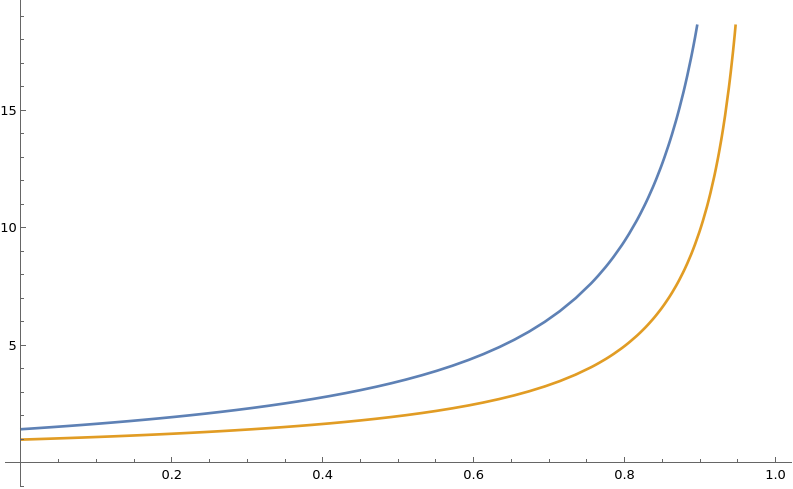
\includegraphics[width=0.75\textwidth]{figures/fig-randomisedwmu}
    \caption{Comparison of the two terms from~\cref{theo:wmu,theo:wmu:rand}: in orange, $\frac{1}{1-\orange{\beta}}$, and in blue, $\frac{1}{\ln\frac{2}{1+\orange{\beta}}}$.}
    \label{fig:mwu:rand:comparison}
\end{figure}
Don't let yourself get fooled by the change of logarithm basis between~\cref{theo:wmu,theo:wmu:rand}: the new bound is always better~--~up to exactly that factor $2$, as $\orange{\beta}\to 1$! (Except, of course, that it is only in expectation).

\begin{framed}
    \noindent\emph{Going further:} for more on this, and connections to online learning and learning theory, see the (excellent) lecture notes by Daniel Hsu, available at \url{https://www.cs.columbia.edu/~djhsu/coms6998-f17/notes.pdf}.
\end{framed}

\bibliographystyle{alpha}
\bibliography{bibliography,extra}
\end{document}
